%%%%%%%%%%%%%%%%%%%%%%%%%%%%%%%%%%%%%%%%%
% Masters/Doctoral Thesis 
% LaTeX Template
% Version 2.5 (27/8/17)
%
% This template was downloaded from:
% http://www.LaTeXTemplates.com
%
% Version 2.x major modifications by:
% Vel (vel@latextemplates.com)
%
% This template is based on a template by:
% Steve Gunn (http://users.ecs.soton.ac.uk/srg/softwaretools/document/templates/)
% Sunil Patel (http://www.sunilpatel.co.uk/thesis-template/)
%
% Template license:
% CC BY-NC-SA 3.0 (http://creativecommons.org/licenses/by-nc-sa/3.0/)
%
%%%%%%%%%%%%%%%%%%%%%%%%%%%%%%%%%%%%%%%%%

%----------------------------------------------------------------------------------------
%	PACKAGES AND OTHER DOCUMENT CONFIGURATIONS
%----------------------------------------------------------------------------------------

\documentclass[
11pt, % The default document font size, options: 10pt, 11pt, 12pt
%oneside, % Two side (alternating margins) for binding by default, uncomment to switch to one side
english, % ngerman for German
singlespacing, % Single line spacing, alternatives: onehalfspacing or doublespacing
%draft, % Uncomment to enable draft mode (no pictures, no links, overfull hboxes indicated)
%nolistspacing, % If the document is onehalfspacing or doublespacing, uncomment this to set spacing in lists to single
%liststotoc, % Uncomment to add the list of figures/tables/etc to the table of contents
%toctotoc, % Uncomment to add the main table of contents to the table of contents
parskip, % Uncomment to add space between paragraphs
%nohyperref, % Uncomment to not load the hyperref package
headsepline, % Uncomment to get a line under the header
%chapterinoneline, % Uncomment to place the chapter title next to the number on one line
%consistentlayout, % Uncomment to change the layout of the declaration, abstract and acknowledgements pages to match the default layout
]{MastersDoctoralThesis} % The class file specifying the document structure

\usepackage[utf8]{inputenc} % Required for inputting international characters
\usepackage[T1]{fontenc} % Output font encoding for international characters
\usepackage{subcaption}

%\usepackage{mathpazo} % Use the Palatino font by default

\usepackage[backend=biber,style=ieee,citestyle=numeric, sorting=nty]{biblatex} % Use the bibtex backend with the authoryear citation style (which resembles APA)

\addbibresource{example.bib} % The filename of the bibliography
\addbibresource{refs_master.bib}
\addbibresource{refs_icpr.bib}
\usepackage[autostyle=true]{csquotes} % Required to generate language-dependent quotes in the bibliography
\usepackage{amsmath,amssymb,amsfonts}
\usepackage{algorithmic}
\usepackage{indentfirst}
\usepackage{sfmath}
\usepackage[export]{adjustbox}
\usepackage{rotating}
\usepackage{mathdots}
\usepackage{yhmath}
\usepackage{color}
\usepackage{float}
\usepackage{multirow}
\usepackage{mwe} 
\usepackage{caption}
\usepackage{subcaption}
\usepackage{lscape}
\usepackage{tikz}
\usepackage{multirow}
\usepackage{pgfplots}
\pgfplotsset{compat=1.8}
\usepackage{pgfplotstable}
\usepackage[normalem]{ulem}
\setcounter{secnumdepth}{3}


%----------------------------------------------------------------------------------------
%	MARGIN SETTINGS
%----------------------------------------------------------------------------------------

\geometry{
	paper=a4paper, % Change to letterpaper for US letter
	inner=2.5cm, % Inner margin
	outer=3.8cm, % Outer margin
	bindingoffset=.5cm, % Binding offset
	top=1.5cm, % Top margin
	bottom=1.5cm, % Bottom margin
	%showframe, % Uncomment to show how the type block is set on the page
}
\DeclareMathOperator{\arctantwo}{\mathnormal{arctan2}}

\definecolor{unlabeled}{rgb}{0.0392,    0.0392,    0.0392}
\definecolor{sky}{rgb}{0.5451,    0.6471,    0.5137}
\definecolor{water}{rgb}{0.3235,    0.5980,    0.73536}
\definecolor{windows}{rgb}{0.7255,    0.7137,    0.4471}
\definecolor{road}{rgb}{0.7216,    0.5804,    0.3412}
\definecolor{car}{rgb}{0.6412,    0.3431,    0.3039}
\definecolor{buildings}{rgb}{0.2980,    0.2980,    0.2980}
\definecolor{none}{rgb}{0.7,0.7,0.7}

\newcolumntype{Z}{>{\setbox0=\hbox\bgroup}c<{\egroup}@{}}
%----------------------------------------------------------------------------------------
%	THESIS INFORMATION
%----------------------------------------------------------------------------------------

\thesistitle{Road Scene Analysis with a multimodal stereovision system} % Your thesis title, this is used in the title and abstract, print it elsewhere with \ttitle
\supervisor{Prof. Fabrice Meriaudeau\\ Prof. Olivier Morel\\ Prof. D\'esir\'e Sidib\'e} % Your supervisor's name, this is used in the title page, print it elsewhere with \supname
\examiner{Rapporteur:\\Rapporteur:\\Examinateur:\\Examinateur:\\Examinateur:} % Your examiner's name, this is not currently used anywhere in the template, print it elsewhere with \examname
\degree{Doctor of Philosophy} % Your degree name, this is used in the title page and ct, print it elsewhere with \degreename
\author{Marc Blanchon} % Your name, this is used in the title page and abstract, print it elsewhere with \authorname
\addresses{} % Your address, this is not currently used anywhere in the template, print it elsewhere with \addressname

\subject{Biological Sciences} % Your subject area, this is not currently used anywhere in the template, print it elsewhere with \subjectname
\keywords{Polarimetry, multimodality, deep learning} % Keywords for your thesis, this is not currently used anywhere in the template, print it elsewhere with \keywordnames
\university{\href{http://www.ubfc.fr}{Universit\'e Bourgogne Franche-Comt\'e}} % Your university's name and URL, this is used in the title page and abstract, print it elsewhere with \univname
\ED{\href{http://http://ed-spim.univ-fcomte.fr/}{\'Ecole Doctorale SPIM}}
\department{\href{http://www.u-bourgogne.fr}{Universit\'e de Bourgogne}} % Your department's name and URL, this is used in the title page and abstract, print it elsewhere with \deptname
\group{\href{http://vibot.cnrs.fr}{VIBOT ERL CNRS 6000 }} % Your research group's name and URL, this is used in the title page, print it elsewhere with \groupname
\lab{\href{http://http://imvia.u-bourgogne.fr//}{ImViA, EA 7535}}
\faculty{\href{http://faculty.university.com}{Faculty Name}} % Your faculty's name and URL, this is used in the title page and abstract, print it elsewhere with \facname


\AtBeginDocument{
\hypersetup{pdftitle=\ttitle} % Set the PDF's title to your title
\hypersetup{pdfauthor=\authorname} % Set the PDF's author to your name
\hypersetup{pdfkeywords=\keywordnames} % Set the PDF's keywords to your keywords
}
\DeclareUnicodeCharacter{0301}{\'{e}}
\begin{document}
\baselineskip=18pt plus1pt

\frontmatter % Use roman page numbering style (i, ii, iii, iv...) for the pre-content pages

\pagestyle{plain} % Default to the plain heading style until the thesis style is called for the body content

%----------------------------------------------------------------------------------------
%	TITLE PAGE
%----------------------------------------------------------------------------------------

\begin{titlepage}
\begin{center}

\vspace*{.06\textheight}
{\scshape\LARGE \univname \\ \LARGE \edname \par}\vspace{1.5cm} % University name
\textsc{\Large Doctoral Thesis}\\[0.5cm] % Thesis type

\HRule \\[0.4cm] % Horizontal line
{\huge \bfseries \ttitle\par}\vspace{0.4cm} % Thesis title
\HRule \\[1.5cm] % Horizontal line
 
\begin{minipage}[t]{0.4\textwidth}
\begin{flushleft} \large
\emph{\textcolor{mdtRed}{Author:}}\\
\authorname % Author name - remove the \href bracket to remove the link
\end{flushleft}
\end{minipage}
\begin{minipage}[t]{0.4\textwidth}
\begin{flushright} \large
\emph{\textcolor{mdtRed}{Supervisors:}} \\
\supname \\% Supervisor name - remove the \href bracket to remove the link  
\emph{\textcolor{mdtRed}{Examiners:}} \\
\examname
\end{flushright}
\end{minipage}\\[1cm]
 
\vfill

\large \textit{A thesis submitted in fulfillment of the requirements\\ for the degree of \degreename \thinspace in Instrumentation and image processing (Instrumentation et informatique de l'image)}\\[0.3cm] % University requirement text
\textit{in the}\\[0.4cm]
\groupname\\ \labname \\ \deptname\\[1cm] % Research group name and department name
 
\vfill

{\large \today}\\[4cm] % Date
%\includegraphics{Logo} % University/department logo - uncomment to place it
 
\vfill
\end{center}
\end{titlepage}

%----------------------------------------------------------------------------------------
%	DECLARATION PAGE
%----------------------------------------------------------------------------------------

\begin{declaration}
\addchaptertocentry{\authorshipname} % Add the declaration to the table of contents
\noindent I, \authorname, declare that this thesis titled, \enquote{\ttitle} and the work presented in it are my own. I confirm that:

\begin{itemize} 
\item This work was done wholly or mainly while in candidature for a research degree at this University.
\item Where any part of this thesis has previously been submitted for a degree or any other qualification at this University or any other institution, this has been clearly stated.
\item Where I have consulted the published work of others, this is always clearly attributed.
\item Where I have quoted from the work of others, the source is always given. With the exception of such quotations, this thesis is entirely my own work.
\item I have acknowledged all main sources of help.
\item Where the thesis is based on work done by myself jointly with others, I have made clear exactly what was done by others and what I have contributed myself.\\
\end{itemize}
 
\noindent Signed:\\
\rule[0.5em]{25em}{0.5pt} % This prints a line for the signature
 
\noindent Date:\\
\rule[0.5em]{25em}{0.5pt} % This prints a line to write the date
\end{declaration}

\cleardoublepage

%----------------------------------------------------------------------------------------
%	QUOTATION PAGE
%----------------------------------------------------------------------------------------


%----------------------------------------------------------------------------------------
%	ABSTRACT PAGE
%----------------------------------------------------------------------------------------

\begin{abstract}
\addchaptertocentry{\abstractname} % Add the abstract to the table of contents
\small{Humans possess an innate ability to interpret scenes under any condition. Computer Vision tends to these capabilities by implementing intelligent algorithms to address complex understanding problems. In this regard, we are interested in understanding outdoor urban scenes in various weather conditions. This thesis specifically addresses the problems arising from the presence of specularity in the scenes. To this end, we aim to take advantage of polarization indices to define such surfaces in addition to traditional objects. In terms of understanding, we aim to introduce polarimetry to the recurrent fields of computer vision and deep learning.
	
	This thesis focuses on the following underlying challenges. First, the estimation of a semantic segmentation at the pixel level is investigated. We exploit polarization cues to define constraints upstream of the convolutional network and thus infuse specularity understanding into the model. As DCNNs are data intensive, we propose the acquisition of a multimodal dataset allowing the comparison of the proposed method with RGB-centric methods. Moreover, to counteract the massive need for data, we establish a procedure to augment the polarimetric informations while maintaining the physical integrity of the information.
	In a second line of research, we address the problem of depth map estimation with a monocular image. Since the algorithms require a colorimetric information, we adapt the processes to an alternative type of imagery. This results in novel regularization terms that allow to accurately infer a depth map from a unique polarimetric image using deep learning. Constrained by the datavore aspect of DL, we build a loss function in accordance with the self-supervision principle. In this manner, we demonstrate the possibility to regularize the depth inference process using terms constraining the normals by relying on polarization. This approach allows us to reconstruct more accurately surfaces observing specular behavior or transparency phenomena.
	
	Ultimately, our two lines of research represent advances towards a more conventional use of polarization in modern computer vision.}
\end{abstract}

%----------------------------------------------------------------------------------------
%	ACKNOWLEDGEMENTS
%----------------------------------------------------------------------------------------

\begin{acknowledgements}
\addchaptertocentry{\acknowledgementname} % Add the acknowledgements to the table of contents
The acknowledgments and the people to thank go here, don't forget to include your project advisor\ldots
\end{acknowledgements}

%----------------------------------------------------------------------------------------
%	LIST OF CONTENTS/FIGURES/TABLES PAGES
%----------------------------------------------------------------------------------------
\tableofcontents % Prints the main table of contents

\addcontentsline{toc}{chapter}{\listfigurename}
\listoffigures % Prints the list of figures

\addcontentsline{toc}{chapter}{\listtablename}
\listoftables % Prints the list of tables

%----------------------------------------------------------------------------------------
%	ABBREVIATIONS
%----------------------------------------------------------------------------------------
%----------------------------------------------------------------------------------------
%	ABBREVIATIONS
%----------------------------------------------------------------------------------------

\addcontentsline{toc}{chapter}{\abbrevname}
\begin{abbreviations}{ll} % Include a list of abbreviations (a table of two columns)
	

\textbf{ASPP} & \textbf{A}trous \textbf{S}patial \textbf{P}yramid \textbf{P}ooling\\
\textbf{CEL} & \textbf{C}ross \textbf{E}ntropy \textbf{L}oss\\
\textbf{DCNN} & \textbf{D}eep \textbf{C}onvolutional \textbf{N}eural \textbf{N}etwork\\
\textbf{DL} & \textbf{D}eep \textbf{L}earning\\
\textbf{DoFP} & \textbf{D}ivision \textbf{o}f \textbf{F}ocal \textbf{P}lane\\
\textbf{HSL} & \textbf{H}ue \textbf{S}aturation \textbf{L}uminance\\
\textbf{IoU} &  \textbf{I}ntersection \textbf{o}ver \textbf{U}nion \\
\textbf{MD} & \textbf{M}ono\textbf{d}epeth\\
\textbf{ML} & \textbf{M}achine \textbf{L}earning\\
\textbf{P2D} & \textbf{P}olarimetry \textbf{2}(to) \textbf{D}epth\\
\textbf{PwSS} & \textbf{P}ixel–\textbf{W}ise \textbf{S}emantic \textbf{S}egmentation\\
\textbf{RGB} & \textbf{R}ed \textbf{G}reen \textbf{B}lue\\
\textbf{SDI} &  \textbf{S}\o rensen-\textbf{D}ice \textbf{I}ndex \\
\textbf{SfX} &  \textbf{S}hape-\textbf{f}rom-\textbf{X}\\

\end{abbreviations}

%----------------------------------------------------------------------------------------
%	PHYSICAL CONSTANTS/OTHER DEFINITIONS
%----------------------------------------------------------------------------------------
% %----------------------------------------------------------------------------------------
%	PHYSICAL CONSTANTS/OTHER DEFINITIONS
%----------------------------------------------------------------------------------------
\addcontentsline{toc}{chapter}{\constantsname}
\begin{constants}{lr@{${}={}$}l} % The list of physical constants is a three column table

% The \SI{}{} command is provided by the siunitx package, see its documentation for instructions on how to use it

Speed of Light & $c_{0}$ & \SI{2.99792458e8}{\meter\per\second} (exact)\\
%Constant Name & $Symbol$ & $Constant Value$ with units\\

\end{constants}

%----------------------------------------------------------------------------------------
%	SYMBOLS
%----------------------------------------------------------------------------------------
%\texttt{}%----------------------------------------------------------------------------------------
%	SYMBOLS
%----------------------------------------------------------------------------------------
\addcontentsline{toc}{chapter}{\symbolsname}
\begin{symbols}{lll} % Include a list of Symbols (a three column table)

$P_\theta$ & polarizer intensity at angle $\theta$ & \si{} \\
$S$ & stokes vector & \si{} \\
$s_n$ & stokes parameter $n$ from stokes vector & \si{} \\
$\bar{s_n}$ & normalized stokes parameter $n$ from stokes vector & \si{} \\

\addlinespace % Gap to separate the Roman symbols from the Greek
\addlinespace % Gap to separate the Roman symbols from the Greek

$\vec{E}$ & electric field & \si{} \\
$\vec{R_w}$ & reflected wave & \si{} \\
$\vec{n}$ & surface normal & \si{} \\

%Symbol & Name & Unit \\

\addlinespace % Gap to separate the Roman symbols from the Greek
\addlinespace % Gap to separate the Roman symbols from the Greek

$\alpha$ & angle of polarization & \si{\radian} \\
$\iota$ & intensity computed from polarization & \si{} \\
$\rho$ & degree of polarization & \si{} \\


\end{symbols}

%----------------------------------------------------------------------------------------
%	DEDICATION
%----------------------------------------------------------------------------------------

%\dedicatory{For/Dedicated to/To my\ldots} 

%----------------------------------------------------------------------------------------
%	THESIS CONTENT - CHAPTERS
%----------------------------------------------------------------------------------------

\mainmatter % Begin numeric (1,2,3...) page numbering

\pagestyle{thesis} % Return the page headers back to the "thesis" style

% Include the chapters of the thesis as separate files from the Chapters folder
% Uncomment the lines as you write the chapters

% Chapter 1

\chapter{Introduction} % Main chapter title

\label{Chapter1} % For referencing the chapter elsewhere, use \ref{Chapter1} 

%----------------------------------------------------------------------------------------

% Define some commands to keep the formatting separated from the content 
\newcommand{\keyword}[1]{\textbf{#1}}
\newcommand{\tabhead}[1]{\textbf{#1}}
\newcommand{\code}[1]{\texttt{#1}}
\newcommand{\file}[1]{\texttt{\bfseries#1}}
\newcommand{\option}[1]{\texttt{\itshape#1}}

%----------------------------------------------------------------------------------------

\section{Context and Motivation}

For the past sixty years, computer vision has been a recurring theme for researchers. With the ambition of making machines "more human", many works tend to allow machines to see and understand similarly to the cognitive capacities of humans. This interest took on even more meaning when learning applications became technologically accessible. The advent of Machine Learning (ML) methods has made it possible to develop increased cognitive abilities applicable to computers and thus to popularize high level domains like scene understanding.

In this thesis we address the problem of understanding scenes but, in addition, we focus on the use of an unconventional modality: polarimetry. Starting from the postulate that the vast majority of efficient methods depend on Red Green Blue (RGB), it seems attractive to try to exploit the knowledge acquired in this space to export it and adapt it to new image modes more suitable to certain situations.
In this perspective, this thesis aims to use polarization to obtain a better scene understanding.
From a global point of view, there are a multitude of approaches to scene comprehension: classification, semantic segmentation, 3D reconstruction, etc. We will particularly tackle the tasks of segmentation and reconstruction. 


Firstly, the semantic segmentation task corresponds to a pixel wise classification of an image. Allowing labels to be assigned at the pixel level as opposed to the image level for standard classification, this area focuses on the semantic aspect. Indeed, the overall objective is to differentiate but also to recognize. The uses of semantic segmentation are diverse and allow, for example, the accurate recognition of humans in an urban environment or the clear delineation of roads (all this in an autonomous vehicle context).
Early approaches such as \cite{ohta1978analysis} allowed the delimitation of the domain as well as its distinction from other approaches of understanding such as classification\cite{agin1980computer}, instance segmentation\cite{edelman1989integrating} etc. Despite a good number of pure image-processing methods, nowadays and in recent years, many methods are based on Deep Learning (DL) and Deep Convolutional Neural Networks (DCNNs). Indeed, the increased learning capabilities as the approaches have evolved have significantly outperformed previously proposed methods. This being stated, the vast majority of contributions on semantic segmentation are now DL-based. 
Requiring a massive amount of data as well as significant computing power, learning architectures allow the translation from an image space to a features space. As a result, networks are capable to learn from data redundancy, the attributes necessary for semantic segmentation. Traditionally, the information provided to these processing modules are RGB images allowing an almost direct discrimination in the color space. However, it is notable that the constraints related to the modality are exported in the network. As follows, the events to which the modality implemented is not sensitive are by extension exported in the DCNN capabilities. 
Many methods have been developed to increase the abstraction capabilities of the networks to overcome data drawbacks. Networks have become deeper and deeper, the number of parameters has increased, features have become more abstract and as a consequence, the requirements in terms of data number and computational capacity have increased.
In this context of semantic segmentation, our intention was to introduce the possibility of using polarimetry as a data source, but also to study whether the change of information could limit the use of greedy and/or datavore methods. Indeed, the idea being to use a different modality to discriminate, prior to the network, the information to drastically reduce the need for feature abstraction.


In a second stage, the reconstruction of 3D scenes represent a radically other domain. The objective is to build a depth map corresponding to the distance between the lens and the objects in the scene. This sub-domain of computer vision is operated for multiple purposes ranging from augmented reality to autonomous navigation and surface analysis. 
Ultimately, this part of the vision is extremely demanding in terms of resources and pre-requisites. Whether it is a Shape from Motion method, stereovision or multiple view geometry, each of these approaches, despite their efficiency, are made complex by their acquisition constraints.
More recently, novel approaches are based on monocular vision and the use of DCNN to estimate depth. In end-to-end manner, the goal is to be able to infer from a simple image a precise depth map. Thus, the more robust these methods are, the less we demand ground truths drawn by LiDaRs that are rendered ineffective during weather alterations. Moreover, as these approaches have evolved, the constraints of supervision have been freed to finally obtain completely self-supervised methods. This has allowed a popularization of the field since it was no longer necessary to maintain an annotated database. Moreover, since depth annotation is generated by tools sometimes rendered inept, some errors could be reduced by generalizing cost functions.
Based on the statement of perspective geometry, the vast majority of approaches are RGB-centric since the visual data are usual and straightforward (colorimetry). This is also explained by the almost unique use of a few datasets like Kitty and CityScapes, which are only available in RGB.
As a consequence, despite similar formulations, non-conventional modalities have not been treated in this field probably due to lack of data. 
Regarding depth map estimation, our goal in this thesis is to incorporate polarization in state-of-the-art methods to take advantage of this data space. 

The overall objective being to operate these algorithms in complex urban areas and/or with altered weather conditions, the polarimetric space is an excellent data candidate. Briefly, since polarimetry is by definition the modality sensitive to reflection phenomena and urban areas are prone to specularity (cars, windows, rain, puddles, etc.), polarization-driven processing units could show increased capabilities.
Therefore, the global intention of this thesis is to merge polarization and current computational tools to benefit from the advantages of both parties. Thus, by moving away from RGB-centric methods, it would be possible to show improved approaches by the specific modality and therefore obtain segmentation and reconstruction methods robust to specularity and weather changes.


We fervently believe in polarization and its discriminative aspects to introduce a further dimension to computer vision algorithms. Combining the knowledge acquired over time with this new data could inject a new impetus to some problems requiring physical understanding. In order to undertake a first step towards these polarization-centric systems, we propose to investigate two fundamental areas of computer vision: segmentation and scene reconstruction. These problems have been chosen as initiators to bring polarization closer to the actual computer vision domain. To such a degree, we aim at popularizing approaches based on polarimetry or any other physics-based vision by demonstrating the usefulness of such a component to traditional approaches.



\section{Scope and Challenges}
This thesis addresses the problem of understanding urban scenes exploiting polarization. Noting the vast majority of algorithms are RGB-centric and suffer from inabilities to categorize certain phenomena, we propose polarization as a discriminant factor to obtain an accurate understanding of urban scenes. By priorly characterizing the scenes in a different space, it is then possible to consider the problems according to various attributes. Consequently, we have investigated the possibilities of understanding urban scenes using polarization cues. Specifically we explored different solutions like learning-based segmentation and deep learning depth reconstruction from a monocular.

\subsection{Pixel-wise semantic segmentation}

The problem of semantic segmentation has been established for a long time. Indeed, it is a question of differentiating the various zones of interest of an image. To address this problem, many methods have been developed.
Whether it is image processing techniques, defining attractive frames and features to delimit the diverse objects of the scenes, or learning-based methods, all have demonstrated the ability of machines to "understand" these particular contexts. Most of these methods rely on the differentiation of textures through RGB-centric systems. This practice assumes texture is a sufficient discriminant to establish a robust segmentation. However, remarkably few methods consider phenomena like specularity. They are often neglected because they are not present in the databases. Indeed, these surfaces have the particularity to observe textureless or saturation computations. One can say that, traditionally, these issues are avoided by the absence of such cases in the images. Since the methods do not observe such occurrences, they are uncharacterized.
Our method does not rely on the textural aspect of the surfaces but rather considers the interaction of these with light.
It then becomes necessary to completely rebuild the segmentation pipeline to move from an RGB-centric to a polarization-centric approach. Consequently, we address the problem of acquiring a reliable database including specular areas traditionally avoided. 
Recently, the use of deep learning approaches has increased the ability to appreciate scenes. We therefore propose implementing this similar kind of approach. Furthermore, we investigate the possibility and viability of operating such models with physics-based vision. 
And since these greedy algorithms require a significant amount of image, we investigate the possibility to increase the size of the database using augmentation processes. In order not to alter the physical and crucial information to the characterization of specularity, we design transformations adapted to infer realistic and physically intact images.

Finally, we propose a complete pipeline, from data to pre-processing to network, of pixel-wise semantic segmentation through deep learning.

\subsection{Monocular depth inference}
To understand the scenes, one can estimate the distance between object and camera. Hence, many methods have emerged to reconstruct 3D scenes. Traditionally, from a monocular, the movement of the camera is necessary to project points in 3D space. Recent approaches have shown that by using learning, many constraints can be avoided. For example, the Monodepth approaches have proven it is possible to infer a depth map from a static image.
Similar to the field of segmentation, these methods are exclusively RGB-centric due to the availability of databases required for such algorithms. As a consequence, some visual phenomena are ignored due to the lack of understanding of these phenomena by the operated modality. Once again, the specularity being however omnipresent in urban areas, it is ignored and directly impacts the genericity of the algorithms.
We then propose evaluating the possibilities of using polarization as a source modality for 3D reconstruction. With the objective of characterizing both diffuse and specular areas, we aim at establishing a set of terms allowing to regularize the inference of a depth map. By infusing polarization cues into the deep learning model, we therefore seek a robust specularity-invarient algorithm, which will reconstruct urban scenes accurately.
To this end, a novel P2D approach is introduced to include these aspects in the monodepth domain. P2D considers both geometric and polarimetric cues to address the depth map estimation problem. The regularization terms can be further exploited to derive innovative approaches and move towards more and more robust methods.

\section{Contributions}
The next section details each work highlighting contributions and associated publications as author \cite{blanchon2019outdoor,blanchon2019utilisation,blanchon2021p2d,blanchon2021polarimetric,blanchon2020intro} or co-author \cite{zhang2019exploration,zhang2019explorationn}.

\subsection{Peer-review publications}
\textbf{Pixel-wise Semantic Segmentation \& Augmentation. }The first major part of our work is presented in Chapter \ref{Chapter4}. Bringing together segmentation and augmentation, the chapter describes the scope of the research conducted to introduce polarimetry in the field of deep learning and also, more specifically, PwSS.
We therefore propose a first of its kind approach allowing to use polarization cues in segmentation which sets the state of the art of the domain. We also demonstrate the usefulness of such information by comparing it with approaches focused on colorimetry. To operate these algorithms, we needed a set of polarization compatible transforms. We subsequently proposed a set of possible augmentations and their corresponding regularization.

Our contributions in this area are primarily motivated by a desire for more recurrent use of polarization in modern computer vision. We then aimed at demonstrating that the characterization of light interactions in a scene is sufficient to accurately determine object classes. Based on the observation that a majority of objects in urban environments are subject to reflection, we then defined a suitable representation to both differentiate objects and depict polarimetry faithfully. 
Due to a lack of data, a multimodal dataset was acquired allowing both training and a fair comparison with similar algorithms on other data. The data being never sufficient, we have also designed augmentation processes allowing to obtain new images respecting the physical integrity of the modality.
Ultimately, a comparative study allowed us to estimate that polarization had an advantage over colorimetry for the segmentation of urban scenes. Moreover, we proved that our augmentation process allowed us to observe superior results. Ultimately, our benchmark on augmentation highlighted that it was preferable not to augment than to augment physics-based images in the usual way without taking into account the physical dimension of the data.\\

\vspace*{8mm}
\hspace*{10mm} ASSOCIATED PUBLICATIONS (SEGMENTATION):
\begin{itemize}
	
	\item "Outdoor Scenes Pixel-wise Semantic Segmentation using Polarimetry and Fully Convolutional Network"\\
	\textbf{Marc Blanchon}, Olivier Morel, Yifei Zhang, Ralph Seulin, Nathan Crombez, D{\'e}sir{\'e} Sidib{\'e}\\
	VISAPP 2019 - \cite{blanchon2019outdoor}
	
	\item "Utilisation de la polarim{\'e}trie pour la segmentation de sc{\`e}nes ext{\'e}rieures avec un r{\'e}seau convolutif"\\
	\textbf{Marc Blanchon}, Olivier Morel, Yifei Zhang, Ralph Seulin, Nathan Crombez, D{\'e}sir{\'e} Sidib{\'e}\\
	ORASIS 2019 - \cite{blanchon2019utilisation}
	
	\item "Exploration of Deep Learning-based Multimodal Fusion for Semantic Road Scene Segmentation."\\
	Yifei Zhang, Olivier Morel, \textbf{Marc Blanchon}, Ralph Seulin, Mojdeh Rastgoo, D{\'e}sir{\'e} Sidib{\'e}\\
	VISAPP 2019 \&  ORASIS 2019 - \cite{zhang2019exploration,zhang2019explorationn}
	
\end{itemize}
\vspace*{8mm}
\hspace*{10mm} ASSOCIATED PUBLICATION (AUGMENTATION):
\begin{itemize}
	\item "Polarimetric image augmentation"\\
	\textbf{Marc Blanchon}, Olivier Morel, Fabrice Meriaudeau, Ralph Seulin, D{\'e}sir{\'e} Sidib{\'e}\\
	ICPR 2020 - \cite{blanchon2021polarimetric}
\end{itemize}
\vspace*{8mm}
\hspace*{10mm} ASSOCIATED COURSE:
\begin{itemize}
	\item "Introduction to Polarization for Rendering and Vision"\\
	Kai Berger, \textbf{Marc Blanchon} - equal contribution\\
		SIGGRAPH Asia 2020 Courses - \cite{blanchon2020intro}
\end{itemize}
\vspace*{8mm}
\textbf{Monocular depth estimation using polarization cues. }The second line of work, presented in Chapter \ref{Chapter5}, corresponds to the estimation of a depth map from a polarimetric monocular. In this chapter we present, to our knowledge, the first approach inferring a depth map from polarization cues using deep learning (similarly to the proposed work on segmentation/augmentation).
We examine the possibilities of loss term regularization to improve the depth maps traditionally deduced from RGB-centric algorithms. As follows, we aim to constrain the problem by formalizing an approach based on the relationship between surface normals and polarization. Since there is no available data, we also propose a polarimetric dataset of dynamic urban areas under different weather conditions. By this way, we aim to categorize the specular areas commonly neglected. 
Ultimately, we propose improvement possibilities since it has been found that our initial approach is not fully generic. This heads us to design different multimodal fusion methods that could be evaluated and should be made viable. \\

\vspace*{8mm}
\hspace*{10mm} ASSOCIATED PUBLICATION:
\begin{itemize}
	\item "P2D: a self-supervised method for depth estimation from polarimetry."\\
	\textbf{Marc Blanchon}, D{\'e}sir{\'e} Sidib{\'e}, Olivier Morel, Ralph Seulin, Daniel Braun, Fabrice Meriaudeau\\
	ICPR 2020 - \cite{blanchon2021p2d}
\end{itemize}
\pagebreak
\vspace*{8mm}
\textbf{Towards scene understanding through polarization cues. }Since we have proposed a number of methods to characterize urban scenes through polarization, we propose integrating all these works into a scene descriptor pipeline. The effort has been produced beforehand to force the use of monoculars in all cases of algorithm establishment. Thus, the fusion of these approaches is possible, starting from a polarimetric monocular, to infer a multidimensional descriptive image composed of segmentation, depth and polarization indices.\\

\vspace*{8mm}
\hspace*{10mm} ASSOCIATED PUBLICATION:
\begin{itemize}
	\item "-"\\
	\textbf{Marc Blanchon}, D{\'e}sir{\'e} Sidib{\'e}, Olivier Morel, Ralph Seulin-, Fabrice Meriaudeau\\
	-
\end{itemize}
\subsection{Open source softwares / datasets}
With the objective of promoting the dissemination and use of our algorithms and this particular data, we offer all of our work in open source:

\begin{itemize}
	\item \textbf{Interpol} - A comprehensive list of interpolation method for polarization. Provides an integrated comparison tool.\\
	\url{https://github.com/BlanchonMarc/InterPol}
	\item \textbf{Pola\_NewtonPolynomial} - Demosaicking DoFP images using Newton's polynomial interpolation python adaptation of the initial shared matlab code.\\
	\url{https://github.com/BlanchonMarc/Pola_NewtonPolynomial}
	\item \textbf{P\_Augmentor} - Augmentation toolbox for polarization. Offer multimodal augmentation possibilities with transformation coherency.\\
	\url{https://github.com/BlanchonMarc/P_Augmentor}
	\item \textbf{AcquisitionFromTopics} - Multimodal synchronized acquisition through ROS.\\
	\url{https://github.com/BlanchonMarc/Ros_AcquisitionFromTopics}
	\item \textbf{PolaBot} - Multimodal RGB / NIR / Polarimetric dataset with segmentation annotation.\\
	\url{https://vibot.cnrs.fr/polabot.html}
	\item \textbf{Dense Alignment Toolbox} - A toolbox allowing for dense multimodal alignement \\
	\url{https://github.com/BlanchonMarc/process-vibotorch/tree/master/Alignment}
	\item \textbf{Vibotorch} - A pytorch wrapper allowing for reproduction of results for the segmentation part of this thesis. Embeding metrics, dataset management, etc.\\
	\url{https://github.com/BlanchonMarc/vibotorch}
	\item \textbf{Segmentation and P2D models} \\
	Models available on demand
	\item \textbf{P2D training and testing algorithms} \\
	Source code available on demand
	\item \textbf{Urban scenes under different weather conditions through polarization} \\
	Dataset available on demand
\end{itemize}
\subsection{Internships supervision}
During this PhD thesis, I had the opportunity to supervise three interns:
\begin{itemize}
	\item Jamilu Sulaiman - Ms Computer Vision - 2019 : \textit{"Polarimetric stereovision approach for 3D reconstruction"}
	\item K{\'e}vin Secret-Morland - Ms Computer Vision - 2020: \textit{"Multimodal fusion with polarization"}
	\item Th{\'e}o Petitjean - Ms Computer Vision - 2020: \textit{"Unsupervised polarimetric image segmentation"}
\end{itemize}

\section{Organization}
This dissertation is divided into the following chapters:\\
\textbf{Chapter \ref{Chapter2}} provides a comprehensive overview of the related works by assessing both the learning-based segmentation field and the depth estimation domain.\\
\textbf{Chapter \ref{Chapter3}} introduces multiple concepts of either polarization and deep learning to avoid redundancies along this manuscript.\\
\textbf{Chapter \ref{Chapter4}} proposes solutions to segment complex urban scenes by using both polarization and deep learning. Due to the constraining framework, this Chapter also presents the respective dependencies of the algorithms such as: dataset construction, alignment, augmentation etc.\\
In addition, Chapter \ref{Chapter4} provides a comprehensive range of evaluations for the different segmentation propositions.\\
\textbf{Chapter \ref{Chapter5}} explores how to infer depth from a monocular polarimetric image. We propose a first-of-its-kind deep learning-based algorithm using polarization cues to derive depth maps. Additionally, capitalizing on the drawbacks of the previous method, we propose a comprehensive evaluation of fusion methods as well as a first step towards RGB and polarization fusion for accurate depth refinement.\\
\textbf{Chapter \ref{Chapter6}} gives the final discussion of this thesis and ideas for future work on the presented problems.


% Chapter 1

\chapter{Litterature Review} % Main chapter title

\label{Chapter2} % For referencing the chapter elsewhere, use \ref{Chapter1} 

%----------------------------------------------------------------------------------------

% Define some commands to keep the formatting separated from the content 


%----------------------------------------------------------------------------------------

\section{Deep Learning-based Semantic Segmentation}\label{soa-sss}

In this section we will discuss different deep learning based segmentation methods. Mostly, a few leading approaches will give an overview of the field.
In Section \ref{seg-in}, an introduction as well as an overview of the research field will be proposed.
Next, in Section \ref{seg1}, we will motivate the choice of these methods by displaying a panel of backbones and networks as well as their respective performances.
Then, in Sections \ref{seg2} and \ref{seg3}, we will learn about methods based on VGG and ResNet respectively, since these are the two most widespread backbones in the domain.
Finally, in Section \ref{seg4}, we will propose a conclusion and a discussion related to the domain.

\subsection{Introduction}\label{seg-in}

Segmentation remain a substantial area of computer vision. It is also historical since it is possible to find contrubutions proposed in the 70's \cite{ohta1978analysis}. The main idea of the domain is to be able to delimit and differentiate objects/areas. Thus, the segmentation can be assimilated to a transposition of an image space to an intermediate space, semantic or not. That is to say that instead of utilizing colorimetric information, the representation is changed to differentiate the areas of interest.\\

{
\begin{tabular}[h]{p{0.05\textwidth}!{\color{gray}\vrule width 2pt}p{0.7\textwidth}}
	 &\textit{Reminder on semantic with respect to segmentation.}\\
	 &\textit{In addition to partitioning the images, knowledge is infused into the algorithm. For example, a simple threshold is a naive segmentation, segmentation by feature group into several classes can be semantic if the feature space is differentiable and the various labels are identified. }\\
\end{tabular}
}\\


Some multiple approaches can be used to perform a segmentation operation, apart from learning-based ones. Indeed, even before the advent of deep learning, it was possible to divide the domain into five subdivisions: region-based, feature clustering-based, edge-based, threshold-based and model-based.

Region-based and edge-based are two subtypes that are significantly correlated \cite{kaganami2009region,chu1990integration}. It is a question of separating the image using descriptors which have the effect of describing the image using contours from which regions can be deduced. As example, \cite{iannizzotto2000fast, sappa2006unsupervised} both proposed edge-based segmentation and \cite{wani1994edge, mukherjee2014region} proposed contour-based approaches. It is explicit these two techniques are highly linked and seamlessly one can shift to the other and vice versa.


The threshold-based techniques \cite{bhargavi2014survey} are quite naive. Whether the level is deduced iteratively or empyrically, this method consists in fixing a value at which the image will be bounded and then binarized. Predominantly, this technique allows to separate areas like the foreground and background or to highlight recognizable objects.


Conversely, feature-based discrimination can be considered as more advanced or complex. It consists in clustering a group of features that have been previously extracted. This domain has been highly investigated \cite{watt1986feature,li2006new,rashedi2013stochastic}. Indeed, this is likely due to the vast amount of information extractors previously developed. As a consequence, researchers have been able to exploit the acquired knowledge and then derive robust segmentation algorithms.


Finally, model-based segmentation consists in adopting descriptive models to differentiate the objects in the image. Thus, models like the Markov Random Fields Model \cite{marroquin2003hidden}, active shape models \cite{van2002active} and active appearance models have been used to segment images\cite{cootes2001active}.


In spite of all these possibilities and their respective robustness, the algorithms remain rather tied to the applications and unfortunately, they are rather rarely generalizable (viz. when they are designed for one task, they rarely adapt to others).


At present, the vast majority of algorithms have shifted into the field of deep learning. This is purely due to the performance observed with this approach. Thus DL usage allows to prevent the creation of a handmade feature space. In addition, DCNNs have proven their generalization abilities. The primary constraint is the amount of data but once this criterion is met, then the networks have such an abstraction capacity it is unnecessary to explicitly constrain the problem. Hence, some algorithms infuse knowledge into the network even if this practice is quite marginal. Preferably, researchers are seeking blocks or layers that will allow to abstract the data to higher degree and render it more understandable for the algorithms. 


\subsection{Major backbones and network: a comparative evaluation}\label{seg1}

In the semantic learning-based segmentation landscape, a large number of methods are available. Indeed, the field is active and in constant evolution. However, it is possible to extract methods that stand out from the crowd. Moreover, among all the methods, a criterion allows to differentiate them: the backbone.


The backbone represents a term that designates the feature extraction structure. It can also be termed — erroneously — encoder and allows to transpose an image from its initial space to a latent space, usually a feature vector. The concept differentiating the term encoder and backbone is the backbone is predominantly used pre-trained and has been proven for feature extraction and thus classification tasks. On the contrary, an encoder is a general term that only designates an architecture that reduces the dimensionality of the data by densifying the information.

From these feature extractors, a vast number of networks have been derived. Therefore, the models have an already proven part for the classification and extraction task. As a reminder, a segmentation network can be summarized as a classification network with a secondary structure to recover the initial image dimension. It is also possible to call a segmentation network a classification network at pixel level.

To determine the most representative networks and their respective backbone, we propose in Table \ref{tab:segmentationSoA} a quantitative analysis of the results from significant networks on a common benchmark: CityScapes \cite{Cordts2016Cityscapes}. The comparison metrics are Intersections over Union (IoU) by classes or categories initially proposed by \cite{everingham2015pascal}. In addition, the CityScapes benchmark proposed to calculate the iIoU which corresponds to the instance-level IoU and is considered more representative of the actual results\footnote{Calculation of specific metrics and benchmark results available at: \url{https://www.cityscapes-dataset.com/benchmarks/}}.

\renewcommand{\arraystretch}{1.2}
\useunder{\uline}{\ul}{}
\begin{table}[h]
	\centering
	\caption[Overview of major approaches highlighting performances on CityScapes benckmark and backbones.]{Overview of major approaches highlighting performances on CityScapes benckmark \cite{Cordts2016Cityscapes} and backbones. \underline{Underlined} and \textbf{bold} respresents respectively overall second best and best. \textit{Italic} is best per backbone.}
	\label{tab:segmentationSoA}
	\resizebox{\textwidth}{!}{%
		\begin{tabular}{llcllccccc}
			\multicolumn{2}{c}{Backbone} &
			&
			\multicolumn{2}{c}{Approach} &
			&
			\multicolumn{4}{c}{Reported performances on CityScapes Benchmark \cite{Cordts2016Cityscapes}} \\ \cline{1-2} \cline{4-5} \cline{7-10} 
			\multicolumn{1}{l}{Name} &
			\multicolumn{1}{l}{Year} &
			&
			\multicolumn{1}{l}{Name} &
			\multicolumn{1}{l}{Year} &
			&
			IoU class &
			iIoU class &
			IoU category &
			iIoU category \\ \hline
			\multirow{3}{*}{VGG \cite{simonyan2014very}} &
			\multirow{3}{*}{2014} &
			&
			FCN \cite{long2015fully}&
			2015 &
			&
			65.3 &
			41.7 &
			85.7 &
			70.1 \\
			&
			&
			&
			SegNet \cite{DBLP:journals/corr/BadrinarayananH15}&
			2015 &
			&
			57.0 &
			32.0 &
			79.1 &
			61.9 \\
			&
			&
			&
			DilatedNet \cite{yu2015multi} &
			2016 &
			&
			\textit{67.1} &
			\textit{42.0} &
			\textit{86.5} &
			\textit{71.1} \\ \hline
			ReNet \cite{visin2015renet}&
			2015 &
			&
			ReSeg \cite{visin2016reseg}&
			2016 &
			&
			\textit{58.8} &
			\textit{-} &
			\textit{-} &
			\textit{-} \\ \hline
			\multirow{8}{*}{ResNet \cite{he2016deep}} &
			\multirow{8}{*}{2016} &
			&
			PSPNet \cite{zhao2017pyramid}&
			2017 &
			&
			81.2 &
			59.6 &
			91.2 &
			79.2 \\
			&
			&
			&
			RefineNet \cite{lin2016refinenet}&
			2016 &
			&
			73.6 &
			47.2 &
			87.9 &
			70.6 \\
			&
			&
			&
			LKM \cite{peng2017large}&
			2017 &
			&
			76.9 &
			- &
			- &
			- \\
			&
			&
			&
			EncNet \cite{zhang2018context}&
			2018 &
			&
			- &
			- &
			- &
			- \\
			&
			&
			&
			DeepLab v2 \cite{chen2017deeplab}&
			2016 &
			&
			70.4 &
			42.6 &
			86.4 &
			67.7 \\
			&
			&
			\multicolumn{1}{l}{} &
			DeepLab v3 \cite{chen2017rethinking}&
			2017 &
			\multicolumn{1}{l}{} &
			{\ul 81.3} &
			{\ul 62.1} &
			{\ul 91.6} &
			{\ul 81.7} \\
			&
			&
			&
			DeepLab v3+ \cite{chen2018deeplab}&
			2018 &
			&
			\textit{\textbf{82.1}} &
			\textit{\textbf{62.4}} &
			\textit{\textbf{92.0}} &
			\textit{\textbf{81.9}} \\
			&
			&
			&
			Mask-RCNN \cite{he2017mask}&
			2017 &
			&
			- &
			- &
			- &
			- \\ \hline
			\multirow{2}{*}{ResNeXt \cite{xie2017aggregated}} &
			\multirow{2}{*}{2017} &
			&
			DShortcut \cite{bilinski2018dense}&
			2018 &
			&
			- &
			- &
			- &
			- \\
			&
			&
			&
			ExFuse \cite{zhang2018exfuse}&
			2018 &
			&
			- &
			- &
			- &
			- \\ \hline
			MobileNet v1 \cite{howard2017mobilenets}&
			2017 &
			&
			FSTSL \cite{xie2018improving}&
			2018 &
			&
			71.9 &
			- &
			- &
			- \\ \hline
			\multirow{2}{*}{MobileNet v2 \cite{sandler2018mobilenetv2}} &
			\multirow{2}{*}{2018} &
			&
			LWRF \cite{nekrasov2018light}&
			2018 &
			&
			\textit{72.1} &
			\textit{-} &
			\textit{-} &
			\textit{-} \\
			&
			&
			&
			Fast-SCNN \cite{poudel2019fast}&
			2019 &
			&
			68.0 &
			37.9 &
			84.7 &
			63.5 
		\end{tabular}%
	}
\end{table}

This evaluation table shows that mainly two backbones are used, namely VGG and ResNet. This is why the next two sections will be dedicated to these backbones and the networks that operate them.

\subsection{VGG}\label{seg2}

VGG \cite{simonyan2014very}, standing for \emph{Visual Geometry Group}, is an image recognition network that was founded in 2015. It can be considered the pioneer in the field of classification and was, until the appearance of ResNet the only viable backbone.
This encoding network is based on small $3x3$ convolutions and is reasonably simple (compared to recent architectures). Similar to all encoders, it allows to reduce the dimensionality of the input data and to densify it to obtain a representative vector, in particular it encodes an image $MxNx3$ into a feature vector $1x1x1000$. Initially and as shown in Figure \ref{fig:vgg}, $M = 224$ and $N = 224$.

\begin{figure}[h]
	\centering
	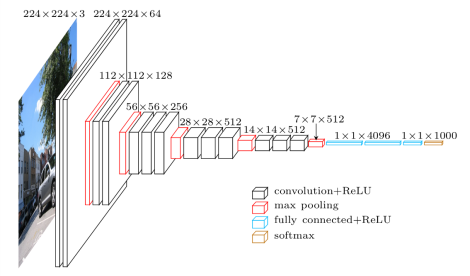
\includegraphics[width=0.5\linewidth]{Figures/SOA/VGG}
	\caption[Simonyan and Zisserman's VGG Architecture.]{Simonyan and Zisserman's \cite{simonyan2014very} VGG Architecture.}
	\label{fig:vgg}
\end{figure}


From its state-of-the-art performances, this network has allowed to derive multiple methods, three of which will be discussed below: FCN \cite{long2015fully}, SegNet \cite{DBLP:journals/corr/BadrinarayananH15} and DilatedNet \cite{yu2015multi}.

\subsubsection{FCN}

\emph{Fully Convolutional Networks} (FCN) \cite{long2015fully}, is an architecture proposed by Jonathan Long, Evan Shelhamer and Trevor Darrell in 2015. It is a highly recognized work to be the "first" pixel-wise semantic segmentation network (PwSS). Wanting to remove the image size constraint, the prevailing idea was to base the architecture solely on convolution layers. Convolution effectively represents a valid technique ensuring the same image size at the output of the pipeline. 
However, the challenge was predominantly based on this dimensionality. As follows, Long et al. proposed an approach based on pooling and deconvolution to retrieve the image dimension while keeping the semantic segmentation information across layers.
While the encoder extracts the information and interprets the image, the decoder considers the task of increasing the dimension while keeping the localization aspect. Only, the effect of downsampling allows reducing the dimension but at the cost of the resolution and the definition when proceeding to the upsampling. In response to this phenomenon, Long et al. introduced the concept of skip connection allowing an aggregation, in the decoder, of information coming directly from the encoder. By this approach, the model is efficient to infer fine-grained segmentation while taking advantage of the dimensionality reduction of the encoder.


\subsubsection{SegNet}

SegNet \cite{DBLP:journals/corr/BadrinarayananH15} is a network highly inspired by FCN but uses other innovative principles. While Long et al. proposed the skip connection concept, SegNet proposes a symmetric architecture with VGG.
And, as a replacement to skip connections, Badrinarayanan et al. develop the principle of indexed pooling. The encoder uses maxpooling operations to reduce the dimension and obtain a feature vector. From this pooling block, an information map of lower dimensionality and an index map is extracted. This index map will then be used in the unpooling operations of the decoder to "reconstruct" the segmentation map with a proper positioning. 



\subsubsection{DilatedNet}

In this approach Yu et al. \cite{yu2015multi}, instead of attempting sampling-based approaches, investigated the concept of dilated convolution. Thus, DilateNet is illustrated by its structure using the dilation properties of convolutions to reduce or increase the size of the maps. The idea is based on this concept of densification of feature maps but also on the increase of the range (i.e. the receptive field) of the convolutions. The advantage is that, for the same impact on the images, the use of dilation allows a much lesser use of parameters and thus the complexity of the networks is decreased by this way. As stated by the authors : \emph{"the receptive field grows exponentially while the number of parameters grows linearly"}.


\subsection{ResNet}\label{seg3}

ResNet \cite{he2016deep} is another backbone and it can undoubtedly be considered as the most widespread in all domains including deep learning based models. The creation of this architecture starts from an observation. Prior to this contribution, the community assumed that the deeper the network, the better it performed. This is legitimate and verifiable, but it is straightforward to observe that in reality, after a certain number of layers, the network loses resolution and performance. This fact comes from a recurrent problem in the learning task: the \emph{vanishing gradient}. After an certain amount of operation, the results are largely approximated by the standard algorithmic methods such as rounding or floating point precision. This would suffer no impact if the training did not require back propagation. Thus, during the propagation, due to the approximation, the floating point estimate \cite{gysel2016hardware} or simply the chain rule \cite{leibniz} used during the calculation of the gradient, the loss shrinks to zero. This vanishing gradient problem prevents the layers from updating and the network does not train anymore.

\begin{figure}[h]
	\centering
	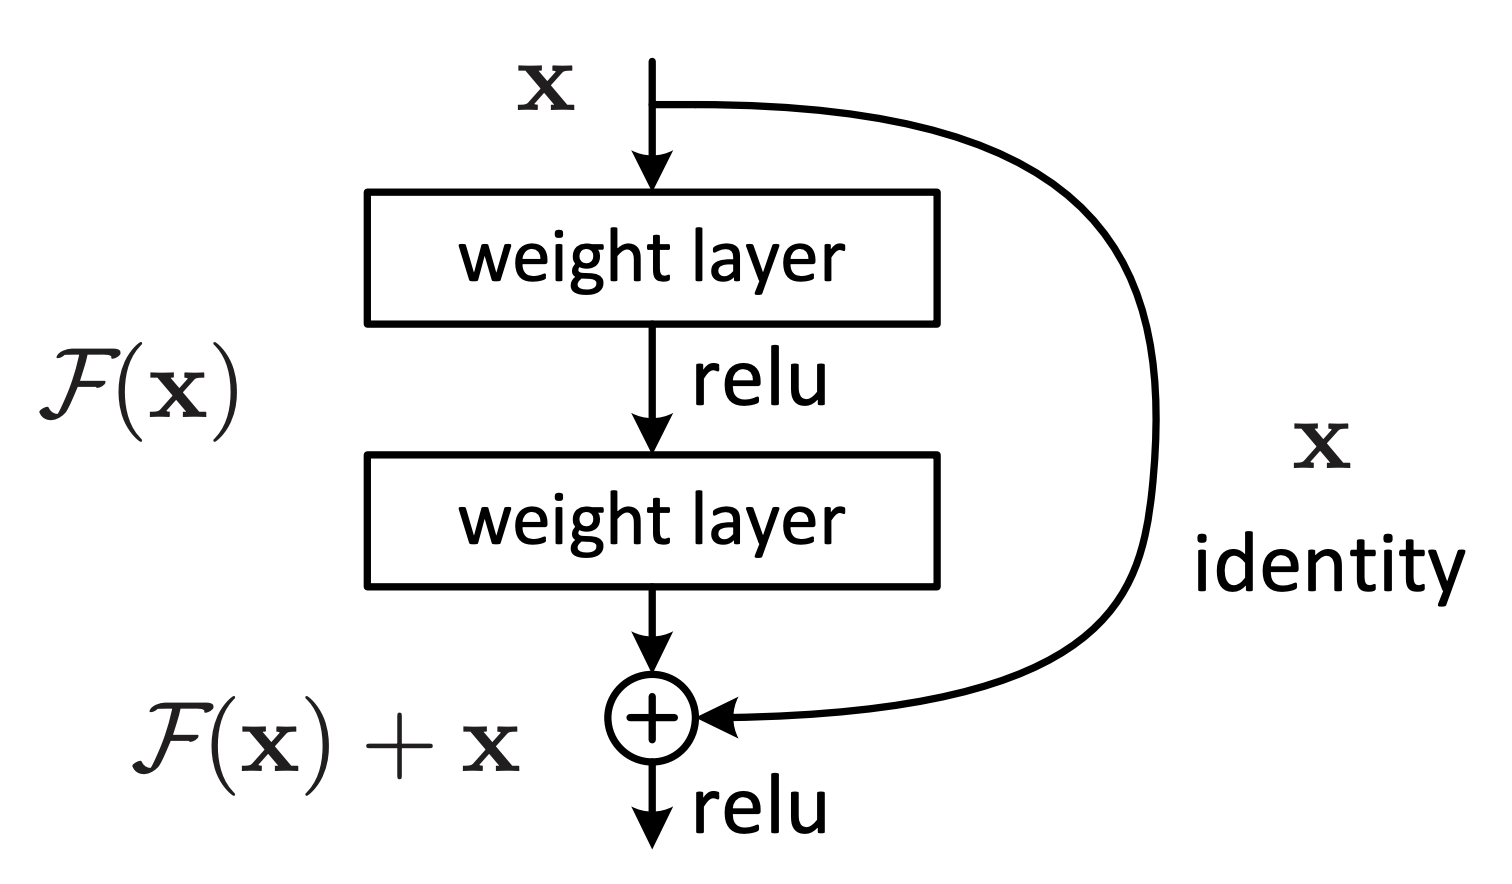
\includegraphics[width=0.6\linewidth]{Figures/SOA/resnetblock}
	\caption[Illustration of ResNet block.]{Illustration of ResNet \cite{he2016deep} block.}
	\label{fig:resnetblock}
\end{figure}


ResNet overcomes this problem by implementing layer-wise skip connections that allow the gradient to be transmitted smoothly (shown in Figure \ref{fig:resnetblock}). By adopting this strategy, it is then possible to use the starting postulate and increase the size of the networks. Once the vanishing gradient is eliminated, nothing prevents the densification of the networks since the skip connections allow the transmission of information.

\subsubsection{PSPNET}

\emph{Pyramid Scene Parsing Network} (PSPNet) \cite{zhao2017pyramid} is a pixel-wise semantic segmentation network derived from ResNet classifiction network. 
This contribution is focused on an innovative sampling method based on a multi-layer pyramid. The approach called \emph{pyramid pooling} is an architecture in four levels (instead of one traditionally). Considered to keep the context of the images, the four stages of the pyramid consider in parallel the whole, half or portions of the base image. Ultimately, whether it is the first feature extraction or the output of each layer of the pooling structure, all this information is adapted in dimensions and concatenated. All this followed by a dense convolution allows keeping both the local and global context of the image and thus to maintain the information across layers. Thus, the loss of information is reduced which allows to have sharp edges and accurate estimations of the classes according to the features extracted by the numerous layers of the network.

\subsubsection{DeepLab}

There are multiple versions of DeepLab. However, it is possible to summarize the ResNet-based contributions into some key concepts brought by Chen et al. \cite{chen2018deeplab}.
First, the global architecture is based on dilated convolutions or atrous convolutions. As expressed for DilatedNet, this operation allows many advantages like dimensionality reduction or judicious management of the receptive field.

Subsequently, this method proposes the use of bilinear interpolation which seems to represent a naive approach to upsampling. In practice, the authors expressed the use of another dimensionality recover strategy is not especially necessary to obtain efficient results.

Ultimately, the contribution proposes the use of \emph{fully connected CRF}. The principle is to consider the pixels as a node in a graph and that all these nodes are connected by different means. Thus, the idea is to enforce the assignment of similar labels to adjacent pixels. The usefulness of this kind of structure could be justified by the classification of areas instead of dependent pixels. Thus, this architecture allows to keep a coherent structure and reduce the aberrations of segmentations with nested classes. In addition, fcCRFs shows great performances with regard to the edges and the object separation.
The contribution of the CRF conveys enormous complexity to the network, but some demonstrations \cite{krahenbuhl2011efficient} has made it possible to remove certain constraints and thus make this type of structure viable.
It is nevertheless considerable this brings a great number of additional parameters and especially increases the complexity of the networks.
To conclude on this architecture that is DeepLab, it remains to this day (with its declensions) the state-of-the-art method for segmentation. Some networks highlight better class-wise performances but include a cost and a disproportionate complexity compared to the difference in efficiency.

\subsection{Conclusion and discussion}\label{seg4}

After briefly explaining the major backbones and their main derived segmentation architecture, it was illustrated that learning-based segmentation has been a flagship field in computer vision. The recorded performances presented in the comparative study are far superior to observations prior to the advent of deep learning. However, it is possible to see this field is almost at the end of its course since the performances tend to stagnate and the research to move towards other processes of understanding. The emergence of instance segmentation or geometric understanding of scenes tends to reduce the amount of contribution in PwSS.

Despite this observation, it is also quite possible to note the algorithms are subject to the same constraints as any deep learning algorithm, namely the need for data. Plus, an overwhelming majority classify colorimetric images and assume these data are thoroughly characteristic of the observed scenes. There is a considerable knowledge in the field of segmentation, but it has rarely been exported to other types of data to see if the performance on similar tasks can be improved by a strategic use of the data.
Hence, the answer might not be to depend on the depth and number of layers of the network but to shift the data space to something more characteristic. 
%----------------------------------------------------------------------------------------
\pagebreak
\section{Depth Estimation}\label{soa-de}

In this section of the literature review, various concepts related to depth will be discussed. Starting from the principal acquisition technology in part \ref{depth-acqu}, we will continue on the learning-less methods for depth estimation in part \ref{multi-im}.
Ultimately, we will more deeply discuss the concept of learning-based depth estimation from a monocular in part \ref{mono-im} since this is the topic on which part of this manuscript is devoted.


\subsection{Laser-based imaging}\label{depth-acqu}

Laser-based imaging is a frequently used method for its accuracy and robustness. Indeed, it allows, regardless of the conditions of illumination or distance, to accurately estimate the distance sensor-object using a laser projection.
There is a wide variety of different sensors, and their performance is highly correlated with their price. Indeed, while some devices allow a smooth acquisition of several thousand points or at distances of several hundred meters, others are relatively limited in capacity. Despite this, the overall acquisition principle remains the same and is uninfluenced by this disparity in performance.
The concept is considerably classic, a laser is projected on a surface that will then reflect it. As follows, it is possible to calculate the distance by measuring the time elapsed between the emission and reception. 
However, the whole principle is based on reflection. As a result, this approach can be inefficient especially when the target scenes include specular surfaces \cite{hrabar2012evaluation} (e.g. mirrors, glass, water, and other reflective surfaces).
It also turns out these sensors can be made deficient in adverse weather conditions. In particular when the projected laser can be refracted in rainy weather or altered in foggy weather.
Conversely, few approaches are as robust in favorable meteorological circumstances. Therefore, most datasets containing target depth maps use laser-based imaging like KITTI\cite{Geiger2012CVPR,Menze2015CVPR,Fritsch2013ITSC} and its LiDaR setup. But, the data contain a bias since they were acquired mainly in favorable conditions.

\begin{figure}[h]
	\centering
	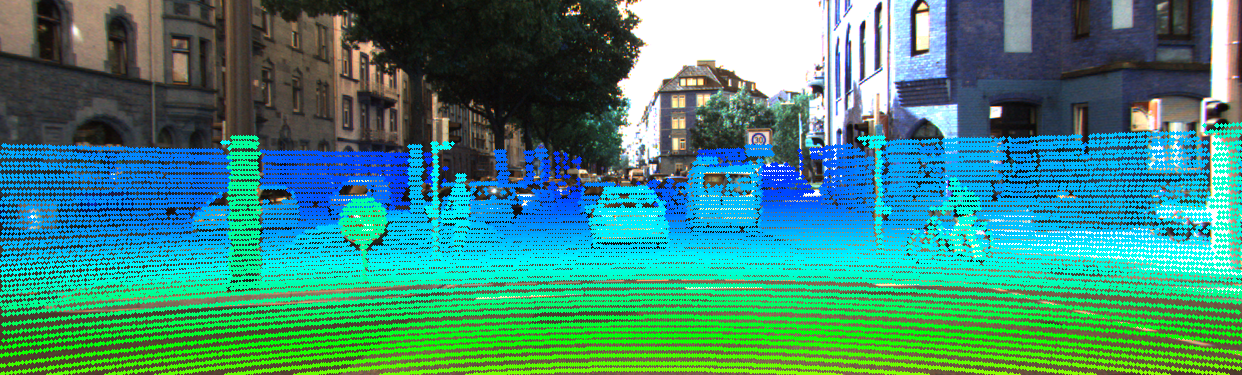
\includegraphics[width=0.8\linewidth]{Figures/SOA/lidar-ill}
	\caption[Illustration of LiDar point-cloud.]{Illustration of LiDar point-cloud\footnotemark. Sparsity can be observed as well as erroneous estimation on vehicle windows.}
	\label{lidar-ill}
\end{figure}



The LiDar, \emph{laser imaging, detection, and ranging}, is a laser rangefinder commonly used since it is motorized and rotatable \cite{wang20133d}. Rotating at 360$^\circ$ at a considerable speed, it allows to make panoramic acquisitions. Moreover, LiDaR are classified according to their number of slices, which gives them, not only a horizontal but also a vertical acquisition. Thus, the more slices, the more vertical points are acquired "semi-simultaneously".
As shown in Figure\ref{lidar-ill}\footnotetext{Image borrowed from \url{henryzh47.github.io}}, the generated point cloud can be affixed to the colorimetric image corresponding to the scene. This illustration also highlights the defects related to specular surfaces, here, the vehicle windows.

In spite of this considerable estimation power, it should be noted that this operation contains flaws of which two critical ones are identifiable. The acquisition of moving objects, especially if the relative speed between sensor and target is high, can be very inaccurate. The second drawback comes directly from the acquisition technology. A multitude of points is projected in the surrounding space. As previously discussed, even if it depends on the size of the pattern, only points are acquired \cite{vaze2007high}. As a consequence, the deduced point clouds are very sparse, and this factor is aggravated by the distance between an object and the sensor (visible in Figure\ref{lidar-ill}). As a result, the depth maps are sparse or subject to interpolation to fill this sparsity.

In conclusion, LiDaR remain a robust tool for scene depth estimation. Regrettably, this device can be expensive or inefficient. As a result, the Computer Vision community tends to find estimation algorithms at the expense of this scanner and its drawbacks.

\subsection{Multi-image methods}\label{multi-im}

Multi-image based depth estimation methods have been developed for several purposes. One of the main ones is the access to this kind of technique since it does not require a complex acquisition system. Indeed, standard cameras can be used to recover the depth. 

These algorithms can be separated in two main parts: Multiple camera systems described in part \ref{mcs}, and Single camera systems in part \ref{scs}.

\subsubsection{Multiple camera systems}\label{mcs}
One of the best-known approaches in the field of multi-camera systems is stereovision. Highly inspired by human biology\cite{marr1979computational}, this technique consists in the use of two cameras similarly to the eyes.

From this acquisition system, two different points of view are obtained and then allow the matching of points of interest. The concept is based on the transposition of points from a three-dimensional space to a two-dimensional image plane.
Hence, starting from a 3D point with homogeneous coordinates, it is possible to transpose it into the image frame such that:

\begin{equation}
	\begin{pmatrix}
	x \\ y \\ 1
	\end{pmatrix} = kP \begin{pmatrix}
	X \\ Y \\ Z \\ 1
	\end{pmatrix},
\end{equation}

with $(x,y,1)^T$ the 2D coordinates and $(X,Y,Z,1)^T$ the 3D coordinates with both ones the scale parameter of the point. Plus, $k$ represents the scale factor and $P$ the projection matrix.

$P$ is a constraining matrix that contains the intrinsic parameters of the camera and the extrinsic parameters. 
These two parameters are respectively the proper properties of the camera independent of any external factor, and the information necessary for the positioning of the camera in the world frame like a $3x3$ rotation matrix and a $3x1$ translation vector.
To find these two parameters, P is decomposed as follows:

\begin{equation}
	P = \underbrace{\begin{pmatrix}
	f_x & 0 & x_0 \\
	0 & f_y & y_0 \\
	0 & 0 & 1
	\end{pmatrix}}_K \underbrace{\begin{pmatrix}
	R_{00} & R_{01} & R_{02} & t_x \\
	R_{10} & R_{11} & R_{12} & t_y \\
	R_{20} & R_{21} & R_{22} & t_z \\
	0 & 0 & 0 & 1
	\end{pmatrix}}_E.
\end{equation}

In this manner, it is possible to retrieve the intrinsic parameters matrix $K$ composed of: $f_x$ and $f_y$ the oriented focal distance in the image, and ($x_0$,$y_0$) the centroptic coordinates in the image frame. In addition, we can recover the rotation matrix $R$ as well as the translation vecotr $t$ with respect to the world frame in the extrinsic parameters matrix $E$. Note, the constraining aspect of $P$ comes from the necessity of these parametric matrices $\{K,E\}$ since this implies a calibration of the system.

\begin{figure}[h]
	\centering
	\begin{subfigure}{.8\textwidth}
		\centering
		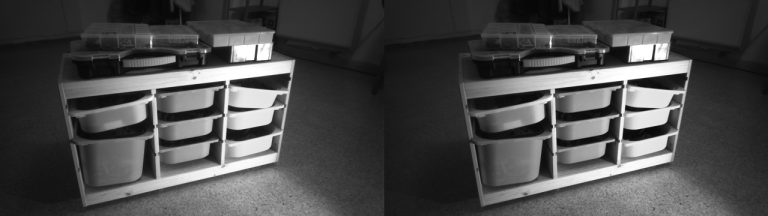
\includegraphics[width=\linewidth]{Figures/SOA/rectified-768x216}
	\end{subfigure}
	\begin{subfigure}{.8\textwidth}
		
		\centering
		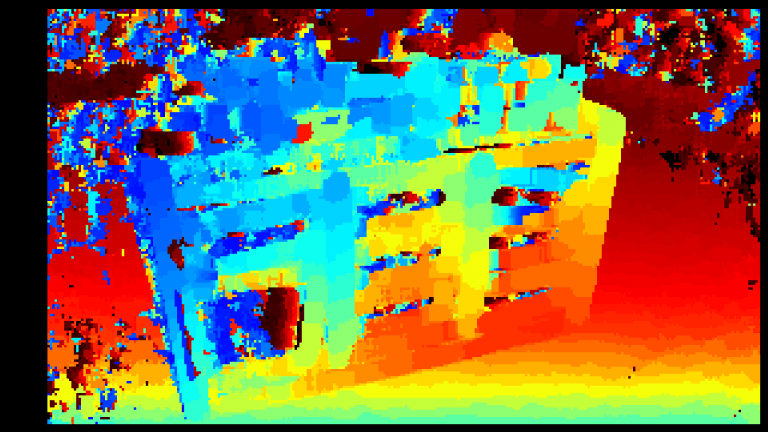
\includegraphics[width=\linewidth]{Figures/SOA/ssd-depth-768x432.png}
	\end{subfigure}
	\caption[Intel RealSense acquisition and reconstruction example.]{Intel RealSense acquisition and reconstruction example. Top row is the rectified images from the camera, bottom row is the obtained reconstruction.}
	\label{intel}
\end{figure}

Conversely, as soon as the sine qua non camera calibration condition is verified, these equations are solvable. This allows us to find the coordinates of 3D points as long as we can identify them in the two or $N$ views. Hence, whether the system is binocular in stereovision as shown in Figure \ref{intel}, or whether the cameras are multiplied in a multi-view system, the problem is reduced to the matching of points identifiable through different views.
As proves \cite{bensrhair1996fast,banks2001quantitative,scharstein2002taxonomy,gehrig2009real} for stereovision, or \cite{hartley1994projective,hartley2000zisserman,campbell2008using} for multiple view reconstruction, this domain has been thoroughly investigated.
Over the years, the research community oriented these approaches towards the real time / online estimation through FPGA embedding \cite{banz2010real}, optimization improvements \cite{kolmogorov2002multi, michael2013real,rodriguez2017improve} or even speed enhancements \cite{feng2019asv}.

Since the system is identified from the stage where it is calibrated, and thus the problem relies almost solely on matching, then many feature differentiation methods have emerged to advance the field.


Thus, different information extraction approaches such as: brightness-based \cite{gennert1988brightness}, segment-based \cite{sumi20023d}, feature-based \cite{se2001vision} or segmentation-based \cite{bleyer2004layered}, have contributed to the progress of multi-image reconstruction.

\begin{figure}[h]
	\centering
	\begin{subfigure}{.3\textwidth}
		\centering
		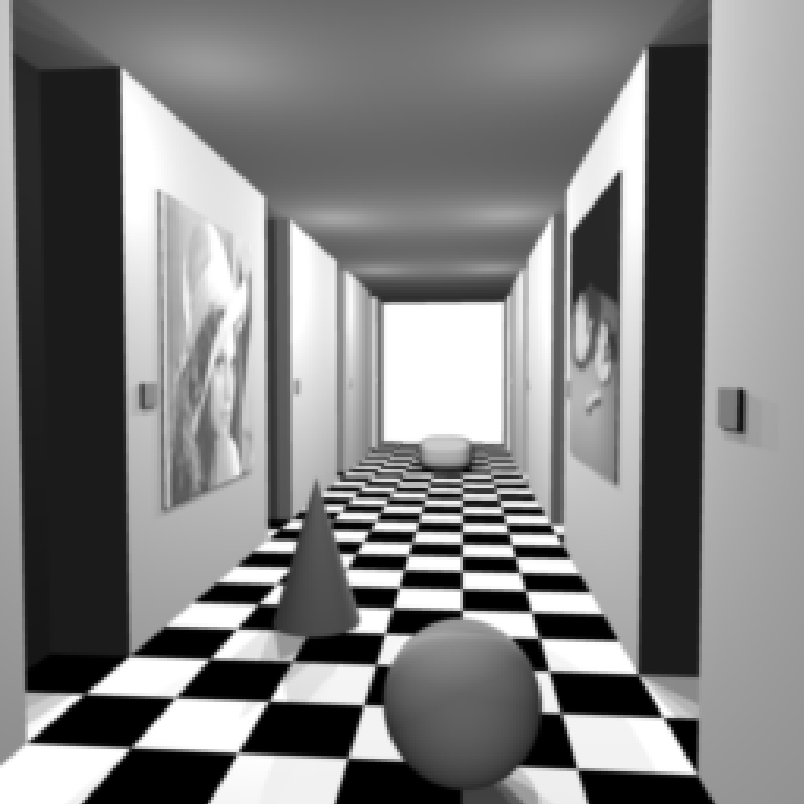
\includegraphics[width=\linewidth]{Figures/SOA/wood1.png}
	\end{subfigure}
	\begin{subfigure}{.3\textwidth}
		
		\centering
		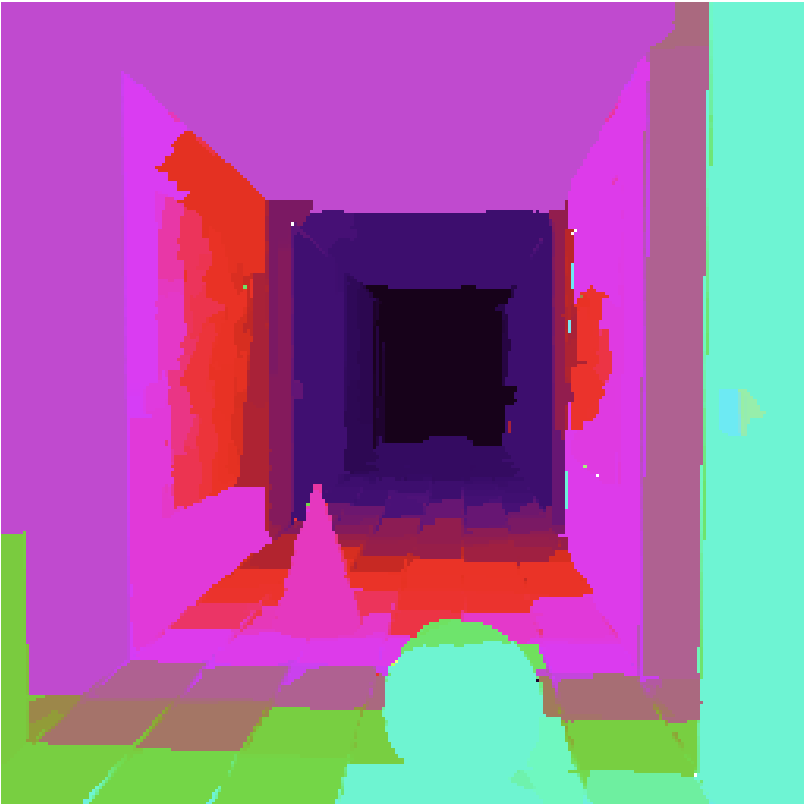
\includegraphics[width=\linewidth]{Figures/SOA/wood2.png}
	\end{subfigure}
	\begin{subfigure}{.3\textwidth}
		
		\centering
		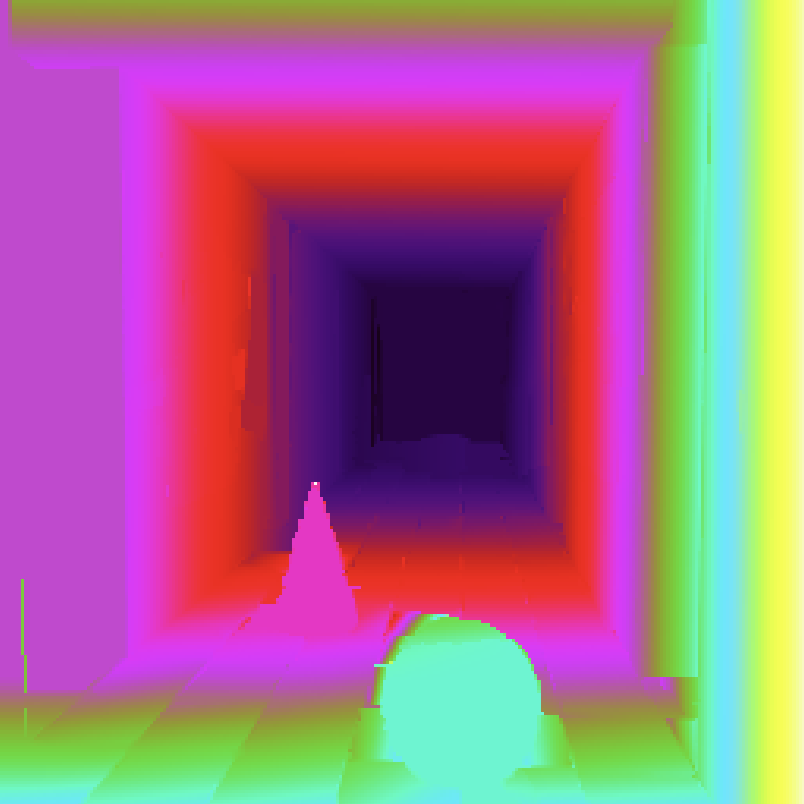
\includegraphics[width=\linewidth]{Figures/SOA/wood3.png}
	\end{subfigure}
	\caption[Illustration of stereovision depth estimation using Woordfor et al. method.]{Illustration of stereovision depth estimation using \cite{Woodford2008GlobalPriors} method. From left to right: reference image, first order reconstruction and second order reconstruction.}
	\label{illu-wood}
\end{figure}

However, to deepen only one contribution, Woordford et al. \cite{Woodford2008GlobalPriors} proposed new optimization approaches leading to leveraging graph cuts to relief surface-orientation major constraint. Therefore, while previous algorithms were struggling while addressing non-fronto-parallel surfaces, they succeeded into integrating second order derivatives leading to more accurate and reliable depth maps. Thus, this method allowed smoother and more precise surface reconstruction in realistic conditions. As shown in Figure \ref{illu-wood}, depth estimation became finer as \cite{Woodford2008GlobalPriors} has been used.

Despite of all the numerous contributions on the multi-image concept and the considerable reconstructions accuracy, still some significant drawbacks subsist. First, as it was discussed above, the calibration aspect represents a key constraint for the acquisition system as well as its deployability. Secondly, as it was highlighted, even if a considerable amount of approaches focuses on features recognition, stereo matching by definition requires features. Unfortunately, the acquisition may observe textureless areas which leads to unsolvable problem. 
Last, the acquisition system requires two or more cameras, and this by essence could be problematic. In response, some methods lift this last constraint by operating a single camera.

\subsubsection{Single camera systems}\label{scs}

Depth estimation from a unique image prevents material constraints but raises other questions. Indeed, the use of such a setup prevents the use of triangulation made possible by the use of multiple sensors.
Therefore, innovative approaches named Shape-from-X (SfX) have emerged. In this framework, X represents several possible cues like motion\cite{caine1993design,dellaert2000structure,chhatkuli2014non,parashar2016isometric}, shading\cite{horn1986variational,zhang1999shape}, blur\cite{favaro2005geometric,zhuo2009recovery}, texture variation \cite{aloimonos1988shape} etc.

As a deepened example, Favaro and Soatto \cite{favaro2005geometric} proposed a original approach to benefit from de-focus phenomenon. 

\begin{figure}[h]
	\centering
	\begin{subfigure}{.3\textwidth}
		\centering
		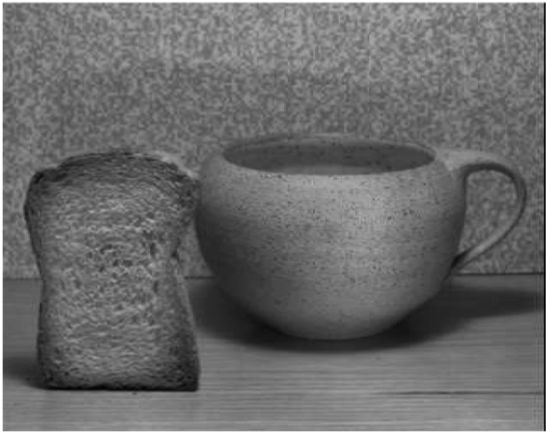
\includegraphics[width=\linewidth]{Figures/SOA/fav1.png}
	\end{subfigure}
	\begin{subfigure}{.3\textwidth}
		
		\centering
		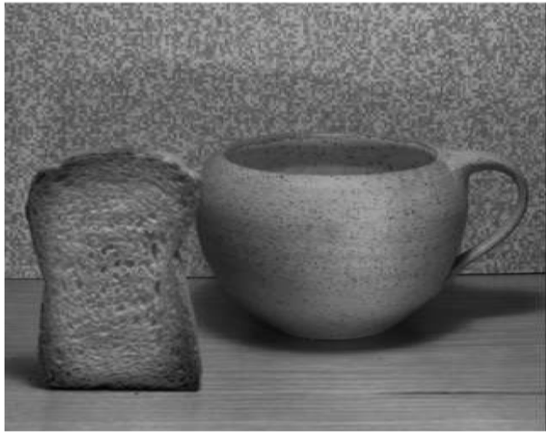
\includegraphics[width=\linewidth]{Figures/SOA/fav2.png}
	\end{subfigure}
	\begin{subfigure}{.3\textwidth}
		
		\centering
		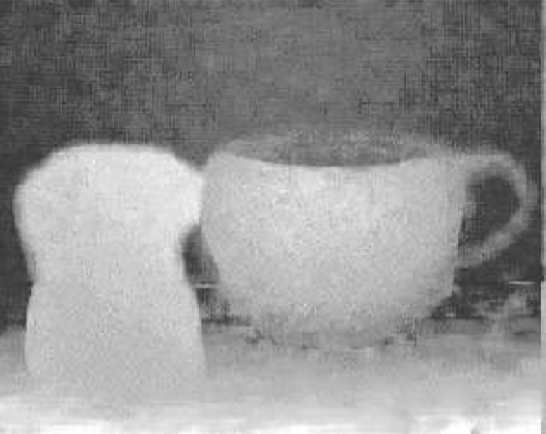
\includegraphics[width=\linewidth]{Figures/SOA/fav-r.png}
	\end{subfigure}
	\caption[Estimate computed from Favaro and Soatto's method.]{Estimate computed from Favaro and Soatto's method \cite{favaro2005geometric}. The two left images shows different images from the focus point of view. The right image display the result of their reconstruction approach.}
	\label{illufavaro}
\end{figure}

The proposition is such that from two images with different camera settings, implying dissimilar focus, they propose computing either:

\begin{itemize}
\item an optimized inference when \emph{point spread function} (PSF) \cite{rossmann1969point} is known
\item kernelized orthogonal operator through convolution
\end{itemize}

to estimate the 3D geometry of the scene. As shown in Figure \ref{illufavaro}, with two acquisition of a scene with different focus (two left images), a depth can be infered (right image) just by a blur-focused algorithm.


\begin{figure}[h]
	\centering
	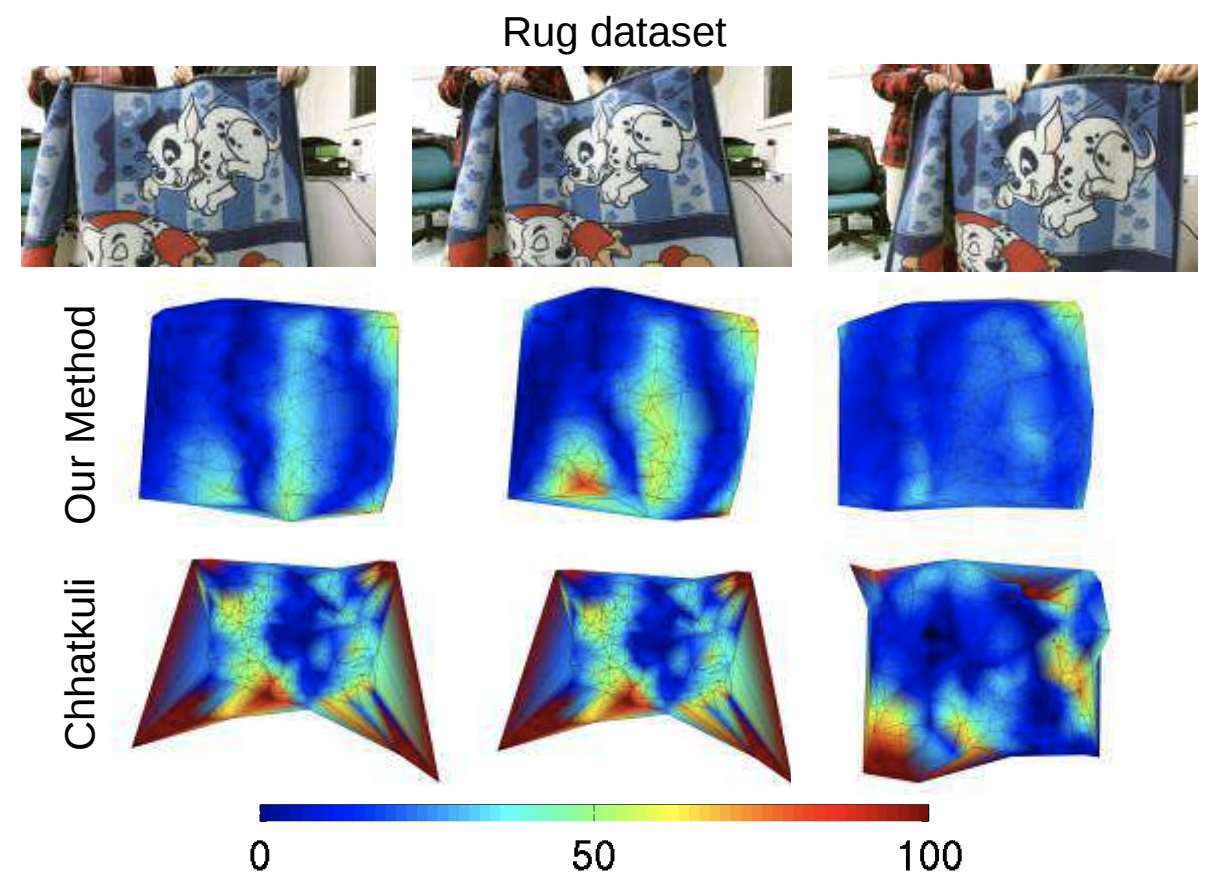
\includegraphics[width=0.8\linewidth]{Figures/SOA/parshar}
	\caption[Example of estimates from Parashar et al.]{Example of estimates from Parashar et al.\cite{parashar2016isometric}. From top to bottom are: input images with deformable object wrapped over time, reconstruction error from \cite{parashar2016isometric} and reconstruction error from \cite{chhatkuli2014non}.}
	\label{illuparshar}
\end{figure}


More recently, Parashar et al. \cite{parashar2016isometric} contributed in the field of shape-from-motion. They propose addressing \emph{Isometric Non-Rigid Shape-from-Motion} which consists of reconstructing a non-rigid object observing shape variation over time. To accomplish such a task, they introduce Riemmanian manifolds-based\cite{lee2006riemannian} representation of the deformable 3D surface. To such a degree, they succeed into modelizing the warps applied to the non-rigid object over time. As shown in Figure \ref{illuparshar}, the proposed method showed increased performances compared to \cite{chhatkuli2014non}.


Despite all these advanced methods, it is considerable that the computational complexity of such algorithms is extremely high. As the sophistication of the algorithms increases, the performance and usability suffer.



In conclusion, despite the fact that the problem of single-camera depth estimation generates an infinite number of solutions and therefore the problem is considered to be ill-posed, the scientific community has been able to adopt innovative approaches to resolve the difficulties. Thus, at the cost of this increased complexity, the acquisition systems could be lightened and SfX field has proposed modern alternatives for depth estimation.
However, the arrival of learning with the growth of computational power has allowed the development of learning-based approaches. 

\subsection{Learning-based monocular depth estimation}\label{mono-im}

In the previous section, we saw it was possible, from several images, whether from one or more cameras, to estimate a depth map. However, each method based on "standard image processing" contains considerable drawbacks. 
With the advent of Deep Learning, many codes has been turned upside down and depth estimation is no exception. Indeed, in essence, learning should relax the constraints by taking advantage of a massive amount of computation. 

These learning-based methods can be divided into two distinct parts, (semi-)supervised learning and self-supervised learning, which will be explained in parts \ref{ssl} and \ref{usl} respectively.

\subsubsection{(Semi-)supervised learning}\label{ssl}

This deep learning process\footnote{Here, the choice was made not to dissociate semi-supervised and supervised learning since they are based on the equivalent concept.} is excessively used as seen in section \ref{soa-sss}, and as for segmentation, for depth estimation, it requires a considerable amount of annotated data. Indeed, as segmentation requires label maps, DCNN-based depth estimation requires reference depth maps.

The problem is thus formulated differently. While previous methods required a characterization of the essential information to match across views, learning-based methods learn by themselves the necessary feature space, provided they utilize a consistent and representative amount of data.

Among the first to investigate the benefit of a profusion of aligned RGB-D data, Eigen et al.\cite{eigen2014depth} were able in 2014 to show that despite an ill-posed problem (as expressed in \ref{scs}), it is possible to obtain sustainable results.

\begin{figure}[h]
	\centering
	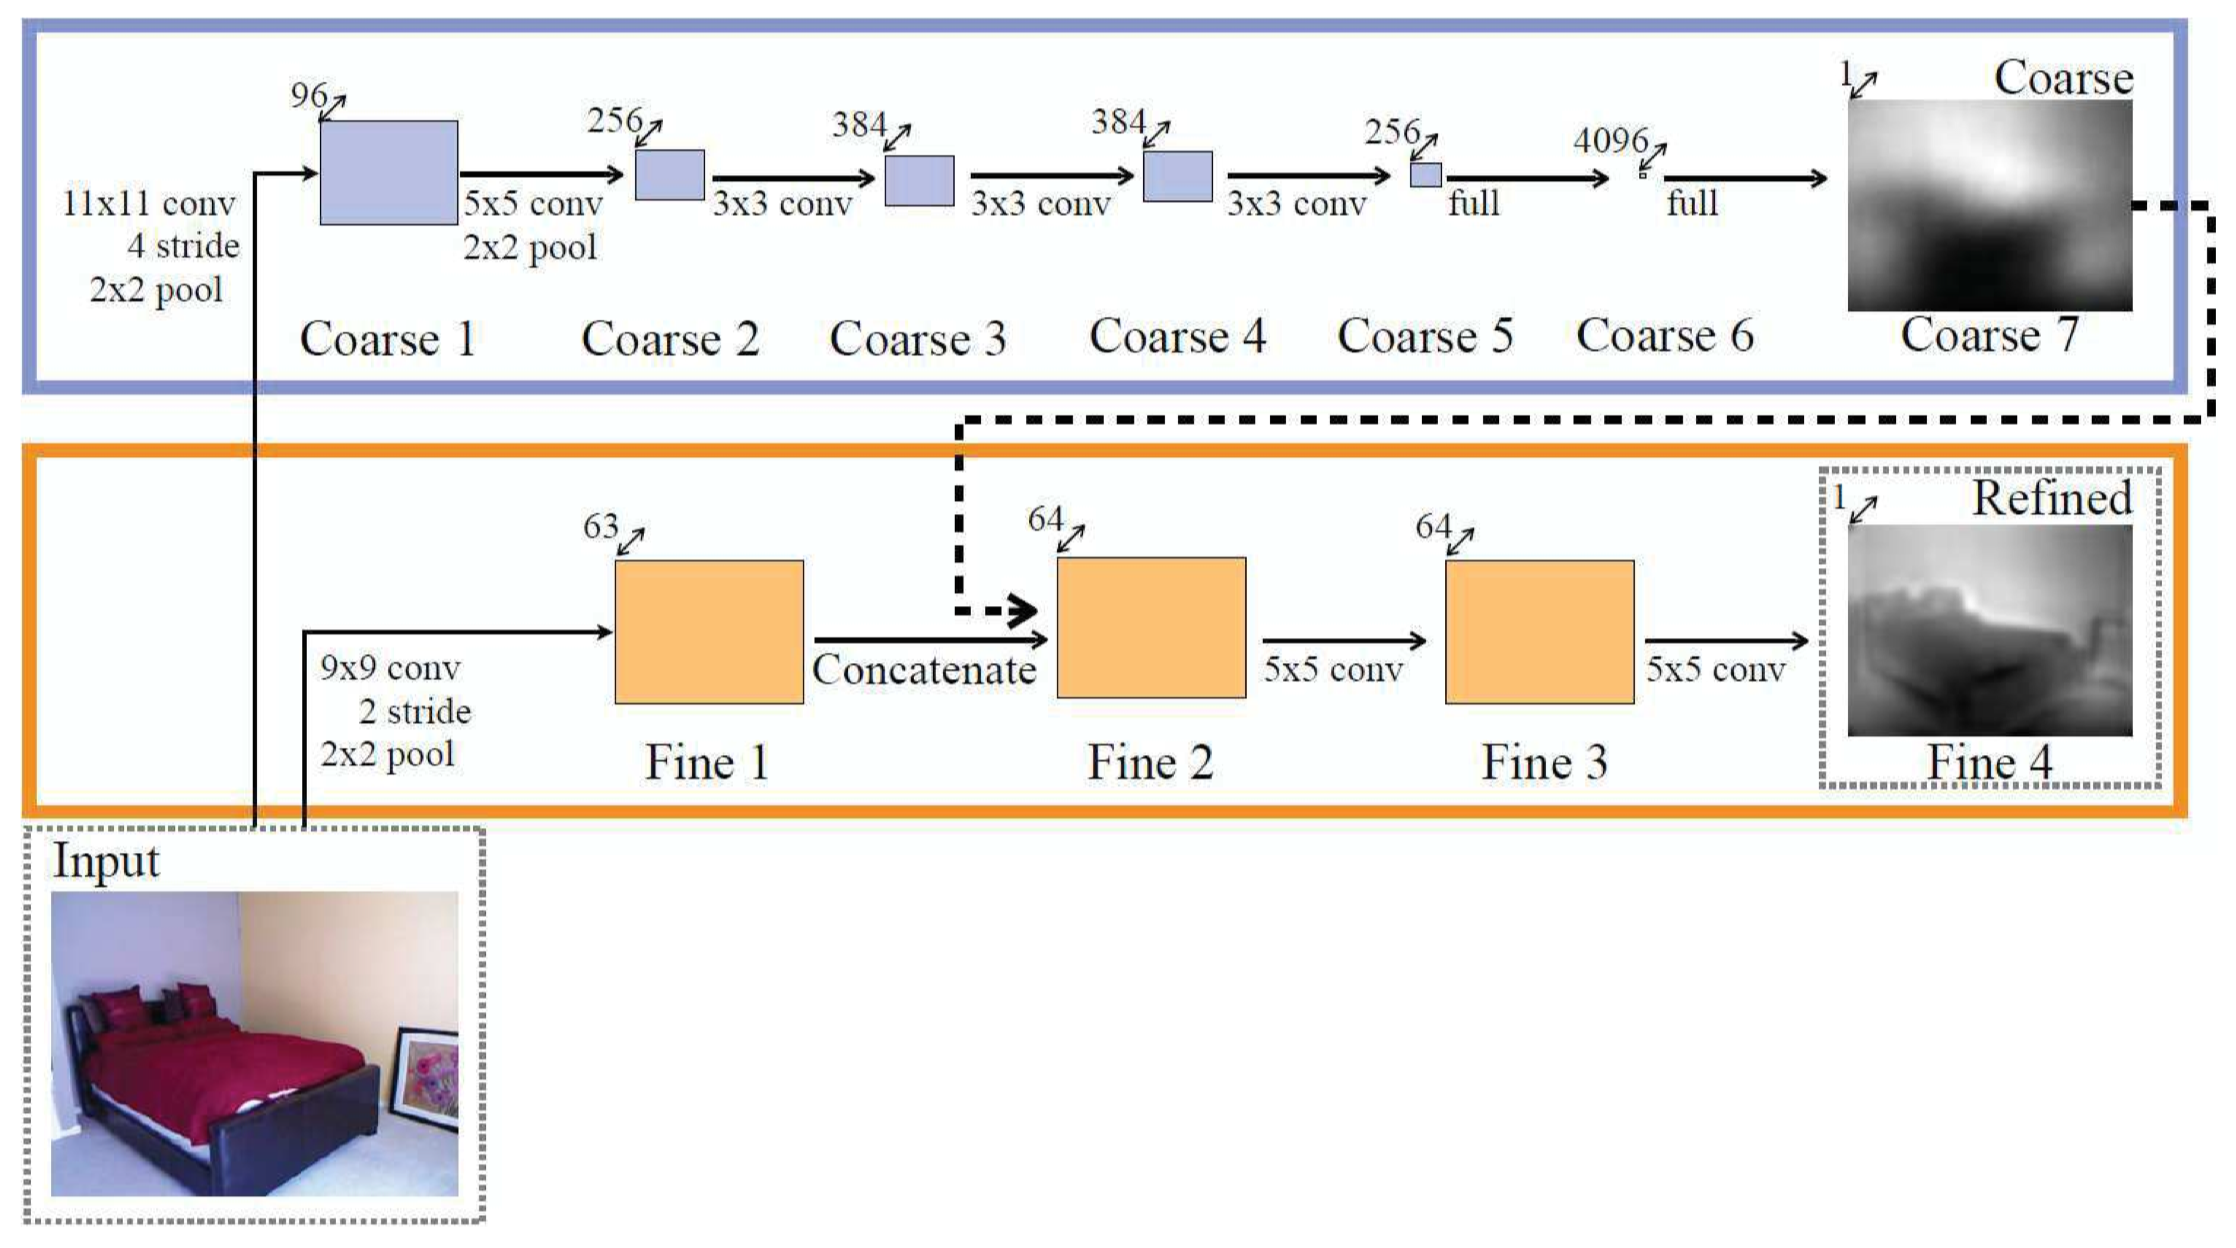
\includegraphics[width=0.8\linewidth]{Figures/SOA/arch-eigen}
	\caption[Eigen et al. Architecture.]{Eigen et al.\cite{eigen2014depth} Architecture.}
	\label{arch-eigen}
\end{figure}


By implementing a biphasic network (shown in Figure \ref{arch-eigen}) allowing the estimation of two depth maps, one coarse and the other refined, while proposing the use of a scale-invariant loss, they were capable to take advantage of rich annotated data sets such as NYU \cite{SilbermanECCV12} and KITTI \cite{Geiger2012CVPR,Fritsch2013ITSC,Menze2015CVPR}.
The contribution is twofold, firstly the cascade network of which the first one, from which the coarse map results, is not completely convolutional (last two layers dense and fully connected). 


\begin{figure}[h]
	\centering
	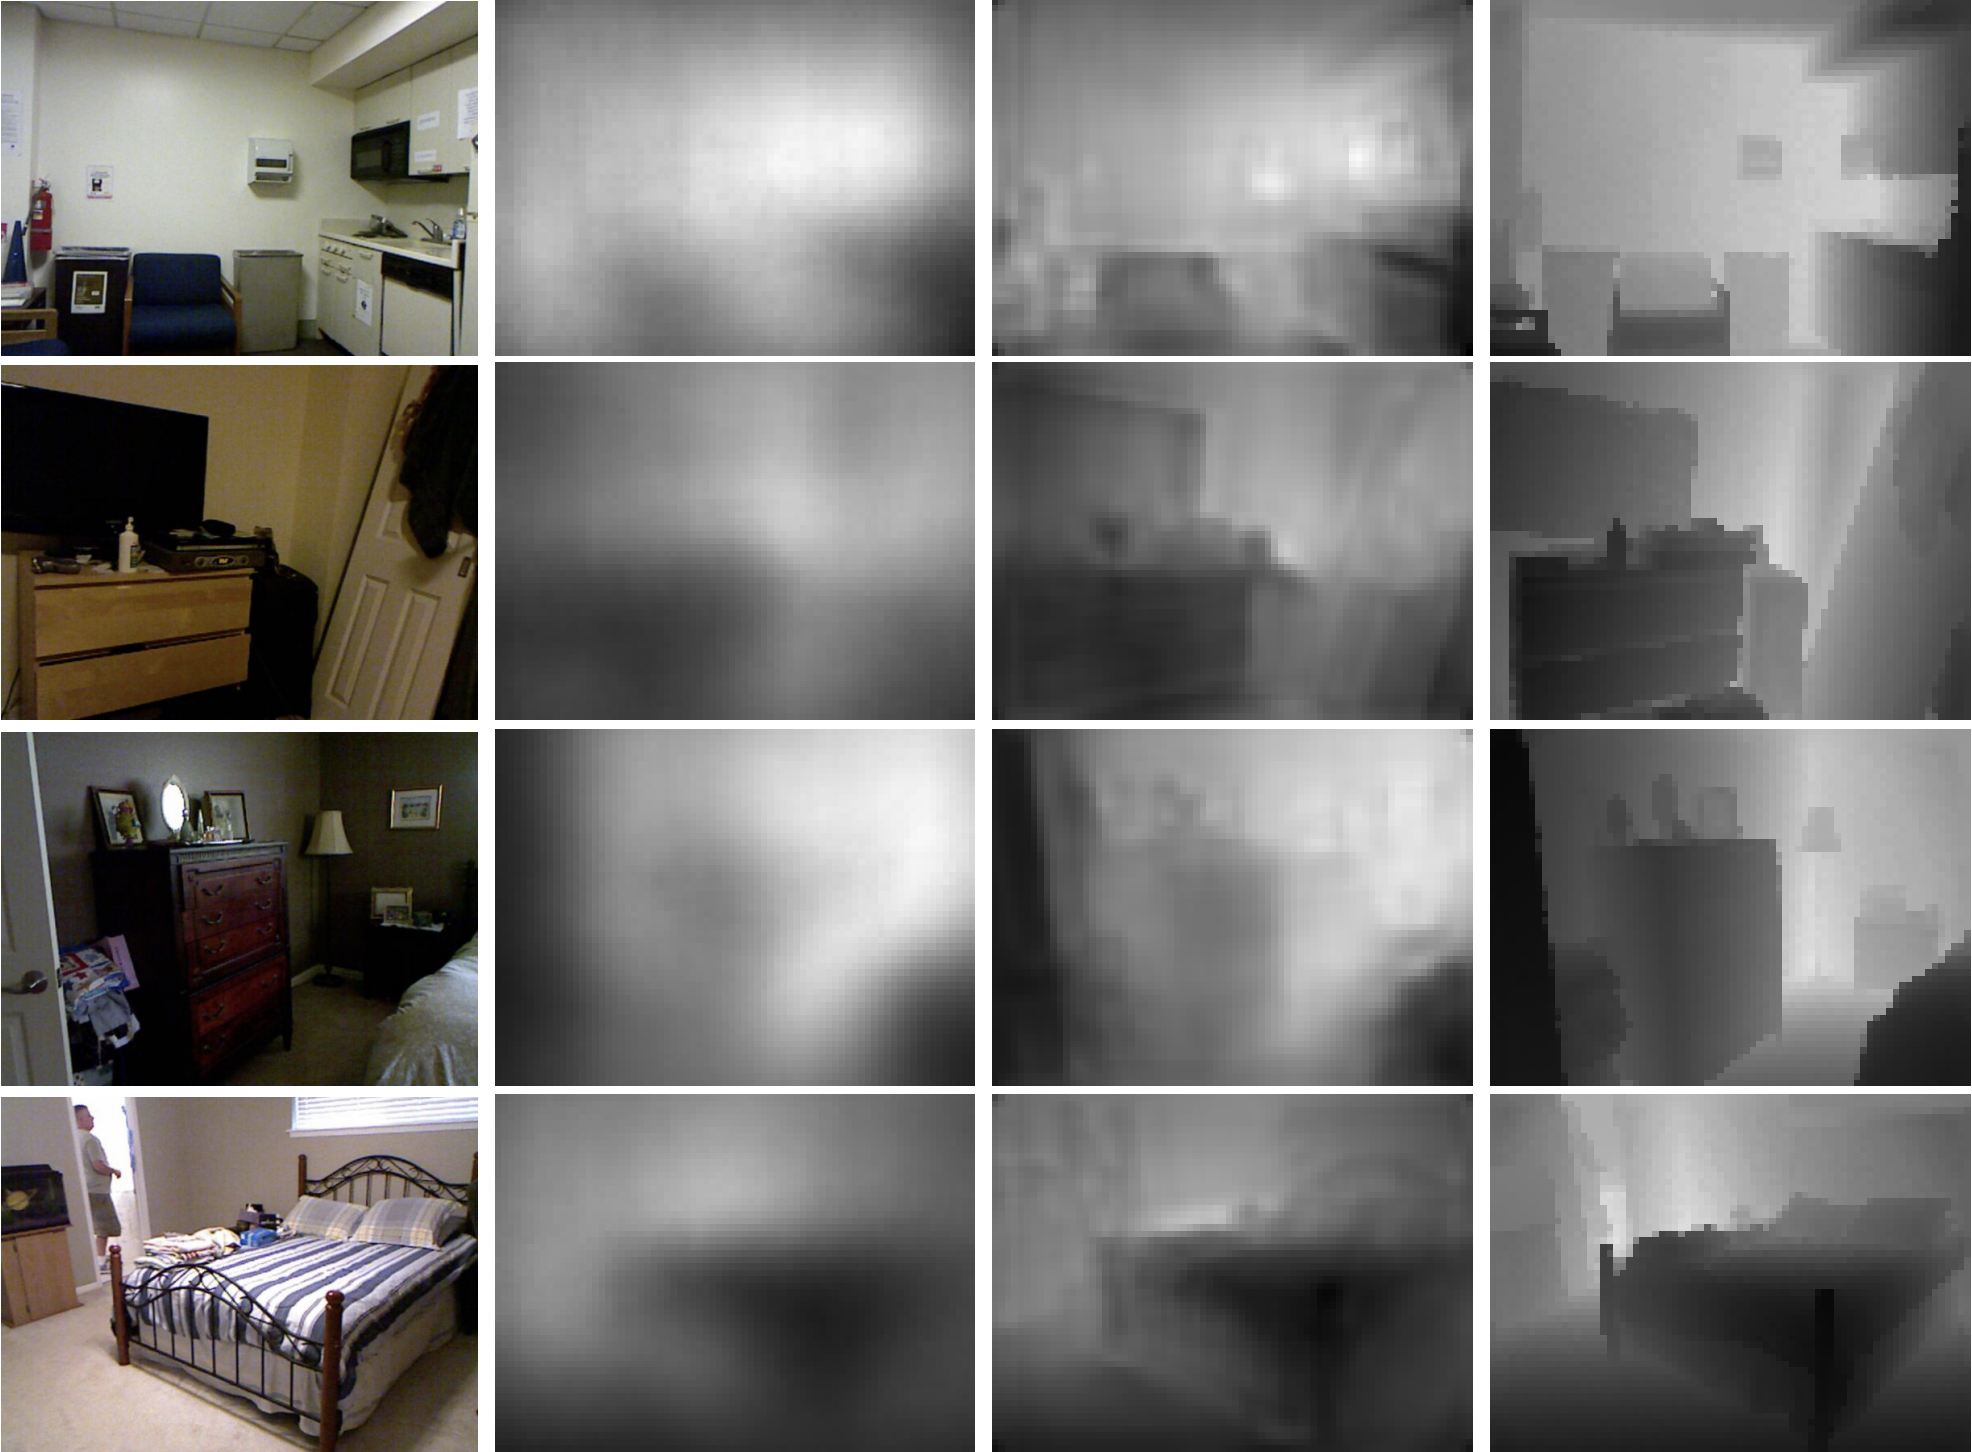
\includegraphics[width=0.8\linewidth]{Figures/SOA/ref-eigen}
	\caption[Eigen et al. Results on NYU dataset.]{Eigen et al. Results on NYU dataset. From left to right: input image, coarse estimation, refined estimation and ground truth.}
	\label{ref-eigen}
\end{figure}

This fact implies the sacrifice of the categorization of local features in favor of a learning of global features. Consequently, this part removes the invariance pose to densify the intermediate latent space.
In a second step, the scale-invariant error allows to introduce a further dimension to the learning. Rather than considering the pixel correspondence by simply using an absolute error, this function allows to partially force the depth relation between pixels. In consequence, the proposed approach is no longer considered as a classification at the pixel level but as an estimation of the depth of the image.
As shown in the Figure \ref{ref-eigen}, the results obtained are impressive and above all will set the state of the art for the field by exceeding all previous performances regardless of the outdoor or indoor environment.


Following this major contribution, this first method has been improved. In 2015, Eigen and Fergus \cite{eigen2015predicting} added the semantic and normals to surface estimation by improving the previous method. Then, using multi-scale approach and by modifying the previous loss, they were able to improve the initial approach. Indeed, while adding a segmentation capability of estimation exceeding previous works, they also were capable to improve their previous outstanding performance.

Next, following these approaches, a multitude of contributions emerged. Liu et al. \cite{liu2015deep} proposed to investigate a joint collaboration between DCNN and continuous conditional random fields (CRF) showing great performance while having an unsmooth patch-like estimation due to super-pixel pre-segmentation for neighborhood relationship modeling.
Another approach is Roy and Todorovic's \cite{roy2016monocular} proposing CNN embedded neural regression tree enforcing the smoothness of output. 
 
\cite{xu2017multi} investigate even more on CRF by introducing a multi-scale dimension to the estimation. Therefore, they created dedicated C-MF blocks which allows multi-scale fusion through the whole process. In consequence, this contribution proved an extensive performance exceeding all the previously cited works.

In addition, as an one-of-a-king approach, \cite{cao2017estimating} proposed to formulate the problem of depth estimation as a pixel-wise classification (can be assimilated as PwSS) problem. Indeed, they suggested the learning task is easier as formulated. As a finality, a CRF is applied to refine the map through local coherency reinforcement.

To cite a few other semi-supervised approaches, \cite{guo2018learning,kundu2018adadepth,fu2018deep,klodt2018supervising}, have all contributed to the growth of the field. 
Whether using a stereovision-based approach, adversarial learning, an ordinal regression formulation or a supervised SfM pre-computation, these methods require at least an intermediate depth estimation step. 

A trend can be observed in the evolution of the field of (semi-)supervised depth estimation. Over the years, the algorithms have benefited from hardware support which has made it possible to evaluate such algorithms, despite their increasing complexity. In contrast, in addition to this prevailing tendency, each of these methods shares a common disadvantage. Indeed, they require a massive amount of annotated data and moreover, these datasets in addition to being consequent must be representative. 
Moreover, most datasets have annotations that depend on the acquisition process. As expressed in part \ref{depth-acqu}, and to consider the example of KITTI, LiDaR is not infallible, especially in urban areas which contain many specular or refractive areas. As follows, when one supervises an algorithm with erroneous data, the model is necessarily influenced.

As a consequence, alternative self-supervised approaches have been developed to emancipate from annotation through a loss that does not require external information.

\subsubsection{Self-supervised learning}\label{usl}

Self-supervised depth estimation represent an extensively active domain in recent years. The concept comes from an observation concerning prior methods: the necessity of a ground truth is extremely restrictive. As mentioned before, in some cases the targets are unreliable enough and their acquisition is expensive.
This field has even metamorphosed from another estimation method to the desire to create labels. In this manner, the ambition of this kind of algorithm is to equal or even surpass the performance of sensors allowing a direct acquisition of this physical information that is the sensor-object distance.
The primary concept is based on the same principles as standard self-supervised learning, i.e. a generalizing, discriminating and differentiating cost function, but also on the necessity of ground truth only for quantitative evaluation. Hence, the algorithms are independent and can exclusively refer to the information they receive or produce to deduce the result by optimizing the loss function.

Fundamentally, the cost functions are similar across algorithms. They predominantly consist of the assembly of several terms of which two are extensively present: the reconstruction term and the smoothing term.

In this section, we will address two diverse types of algorithms: self-supervised stereo-based supervision and self-supervised monocular-based supervision. In the repertoire presented here, we will consider that the method is considered monocular if its inference is made monocularly. Consequently, some algorithms requiring two views for the learning period will remain valid for our selection criteria. 
In addition, a quantitative evaluation sub-part will display the different algorithm performances on the KITTI dataset's eigen split. This benchmark remain the reference in the domain as well as being freely available since it represents the comparison sample for the community.
Last, the last sub-part will summarize and draw conclusions on the field to position the contributions of this manuscript in this research landscape.

\textbf{Self-supervised stereo-based. } This subpart of monocular depth estimation relies on a key point which is the training with a stereo image pair. These approaches are almost all based on the principles mentioned in section 1, with the difference that the processing core is a DL network and that consequently the loss and the images are sized for this computing node. 


In 2016, Garg et al.\cite{garg2016unsupervised} proposed an image reconstruction loss-based training procedure to infer depth. Founded on an auto-encoder architecture, their approach predict an inverse-depth image which then derive an inverse warp allowing a photometric error between this synthesized image and the primary one.
\begin{figure}[h]
	\centering
	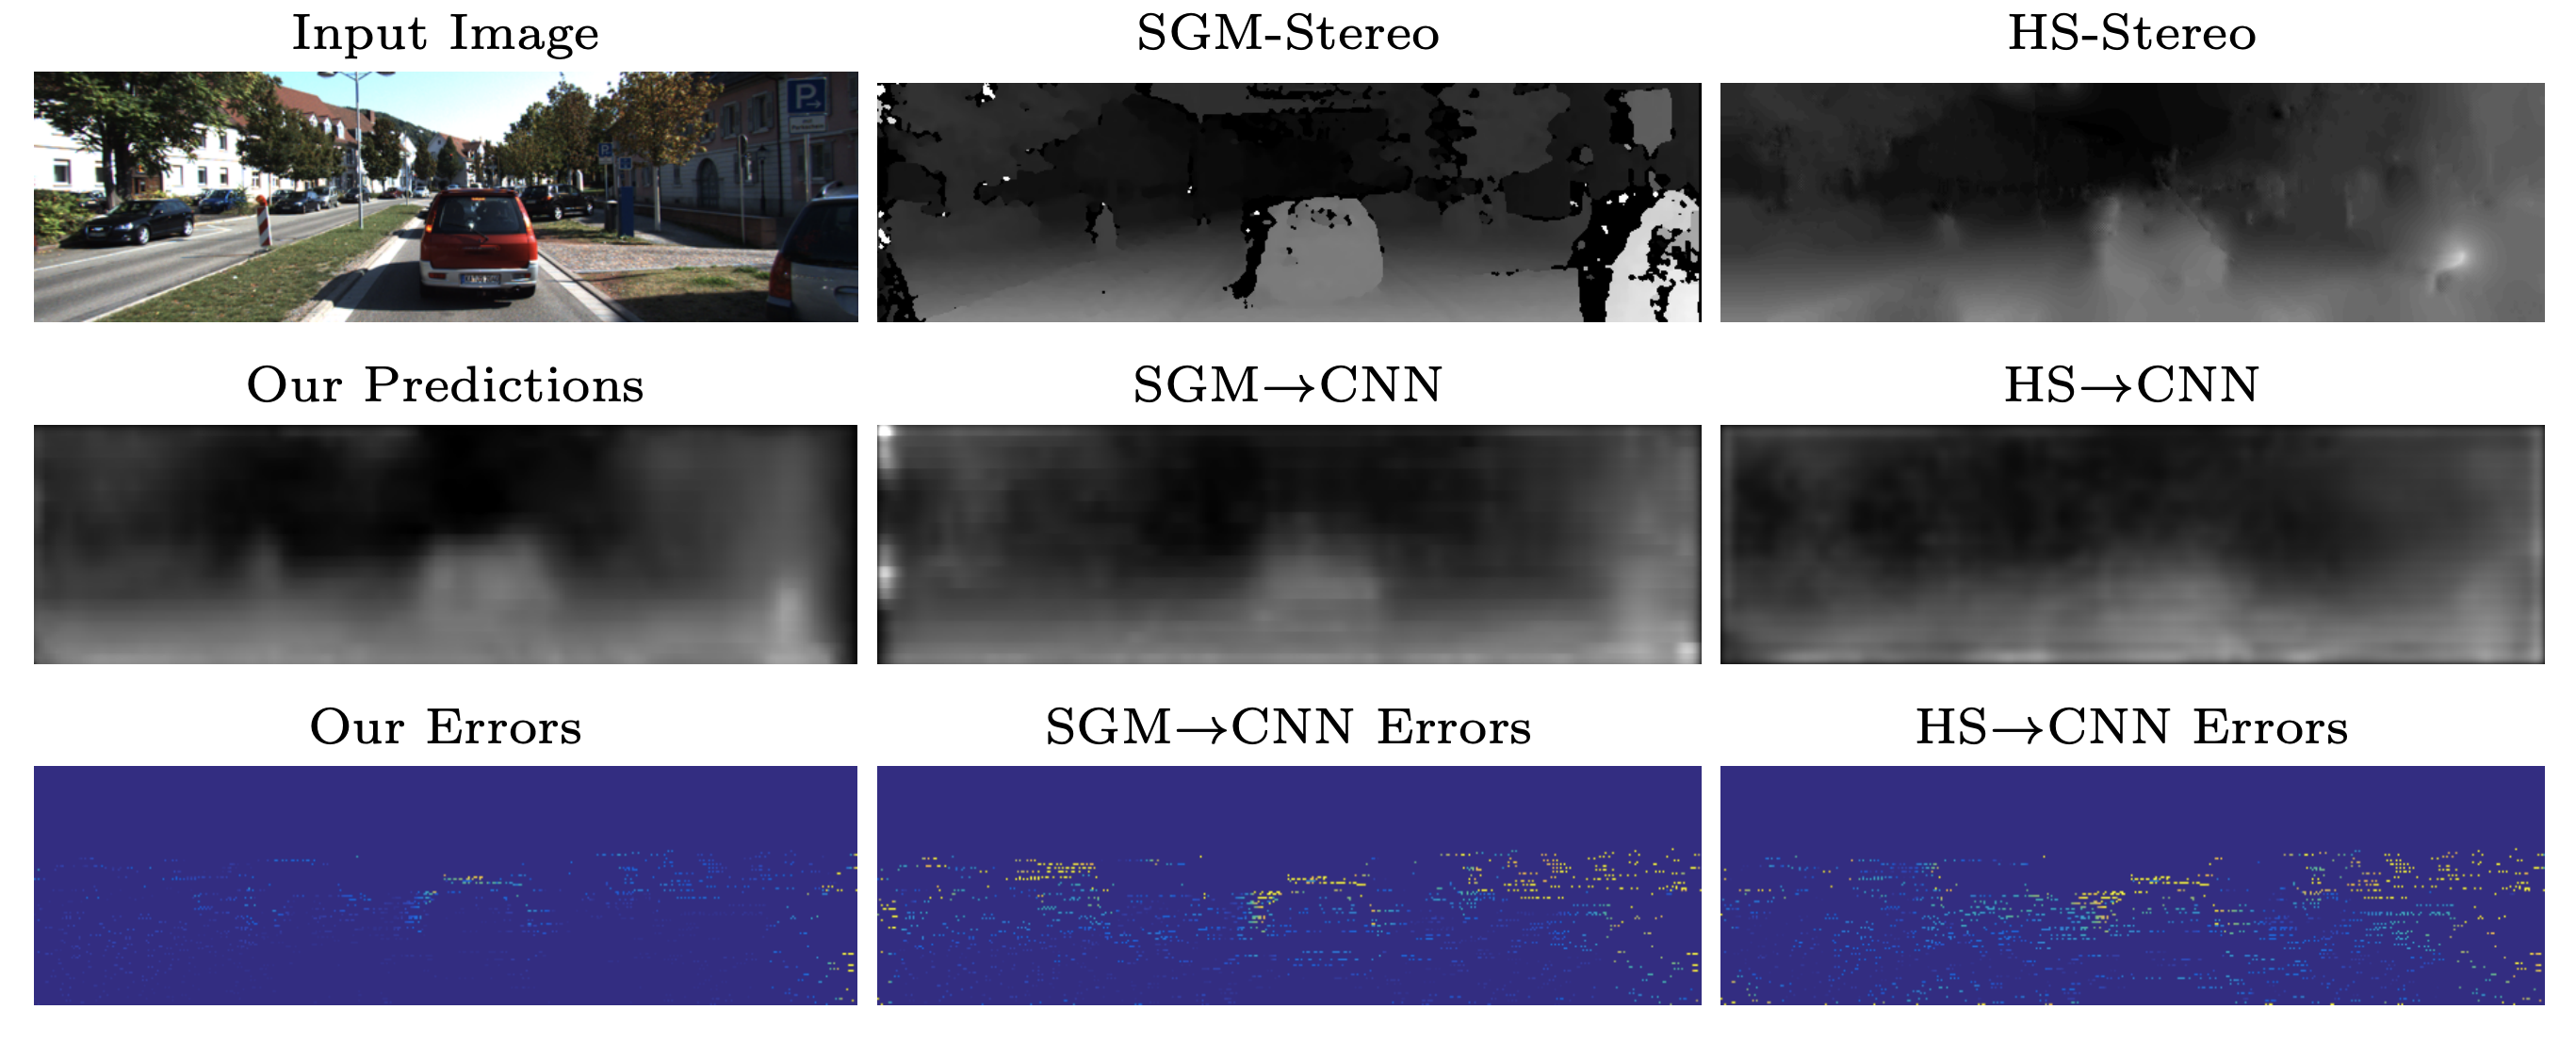
\includegraphics[width=0.8\linewidth]{Figures/SOA/illugarg}
	\caption[Results proposed by Garg et al.]{Results proposed by Garg et al. \cite{garg2016unsupervised} highlighting error reduction compared to other methods.}
	\label{illugarg}
\end{figure}


Although this pioneering approach offers advantages, their image generation-dependent minimization method is undifferentiable. Consequently, at the cost of an increased optimization complexity, they require the use of Taylor approximation to linearize their deformed image and hence, allow the computation of a gradient. As shown in Figure \ref{illugarg}, this approach displayed accurate performances explicitly comparing to direct competitors semi-global matching \cite{hirschmuller2007stereo}.


One year after, \cite{godard2017unsupervised} brings the left-right consistency concept as a term in the minimizable loss. Simplifying, the method consists in generating an opposite image. Using the spatial transformer network and its sampling blocks \cite{jaderberg2015spatial}, this consists of reformulating the perspective geometry statement by recreating a projection.

\begin{figure}[h]
	\centering
	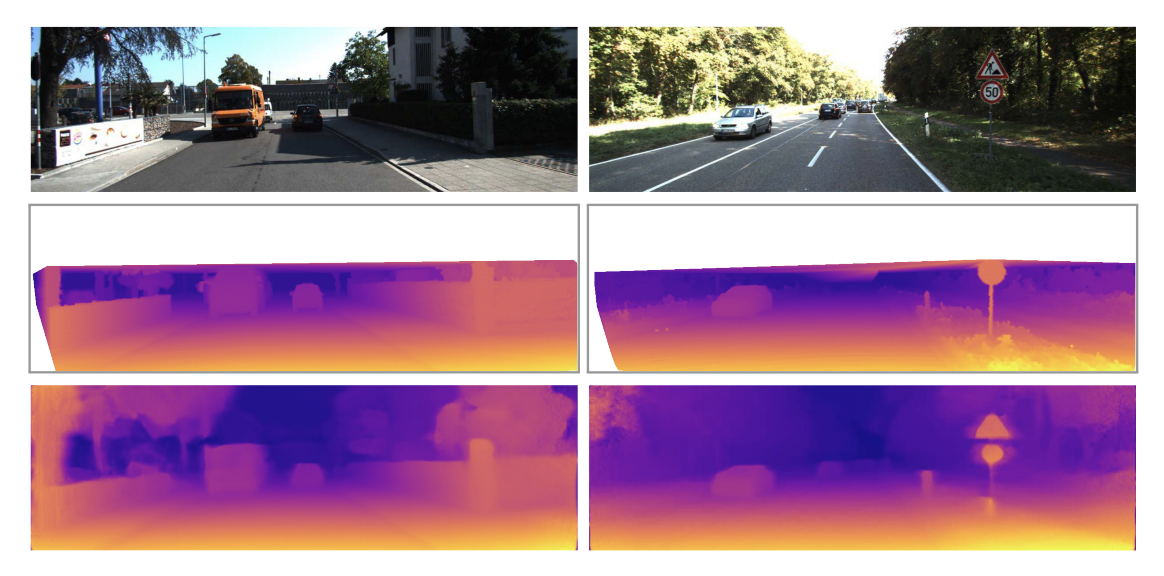
\includegraphics[width=0.8\linewidth]{Figures/SOA/illugod1}
	\caption[Godard et al. qualitative results.]{Godard et al. qualitative results.}
	\label{illugod1}
\end{figure}


Moreover, Godard et al. propose to complexify the smoothness function to include an \emph{edge-aware} effect that avoids edge blurring. For information, the smoothness term allows attenuating the discontinuity in the estimation due to the gradient of the image. This contribution proposes the addition of a third term called \emph{Left-Right Disparity Consistency Loss} ensuring equality between the first view and the second view projected with the deduced disparity. As shown in the qualitative evaluation presented in \ref{illugod1}, the predicted depth succeed into inferring depth while preserving smooth transitions along distance and salient edges.


Investigating a radically different proposal, \cite{mehta2018structured} suggests the possibility of generating depth maps using Generative \emph{Adversarial Networks} (GAN) \cite{goodfellow2014generative}. As shown in Figure \ref{illumehta}, from an input RGB image, a generator will infer a depth map which then will be discriminated.

\begin{figure}[h]
	\centering
	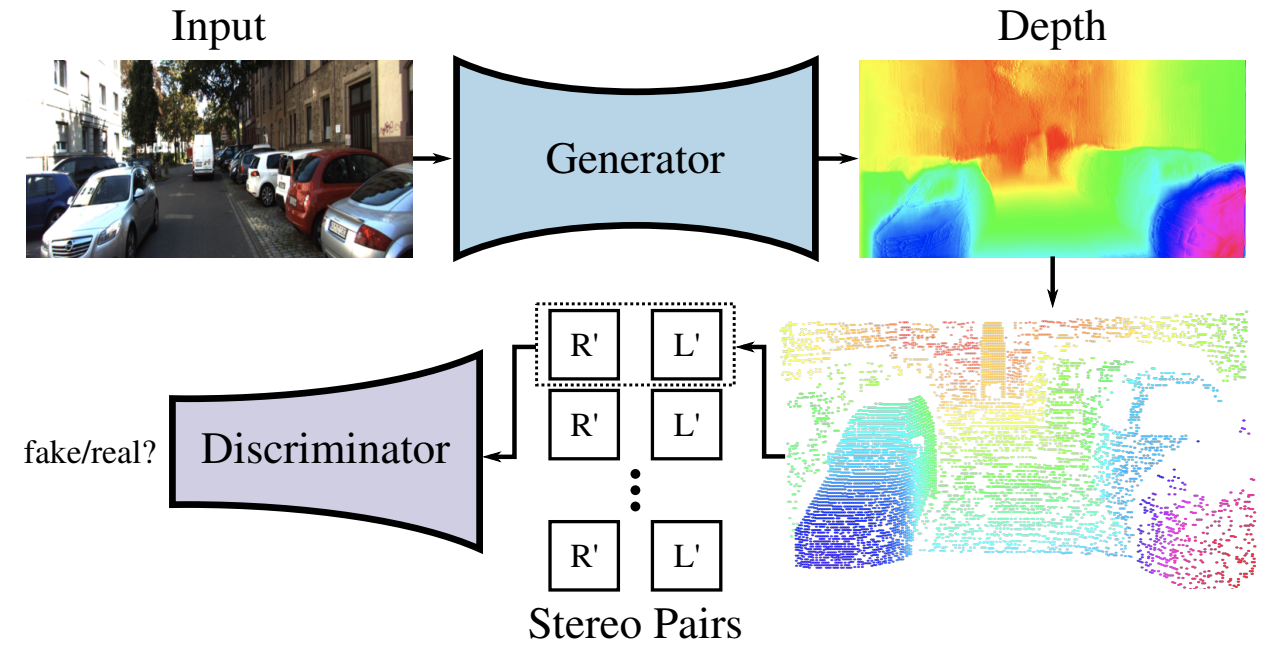
\includegraphics[width=0.8\linewidth]{Figures/SOA/illumehta}
	\caption[Mehta et al. GAN Architecture.]{Mehta et al. GAN Architecture.}
	\label{illumehta}
\end{figure}

The concept of GAN initially consists in the synthetization of photo-realistic images. Within the framework of this approach, it is a question of transposing the space of the colorimetry to the depth. Consequently, the discriminator is improved to ensure a valid estimation. To do so, the task of this network is to distinguish whether a generated view is plausible with reference to the real image collection. Once this network is valid, Mehta et al. train the generator that will produce the depth images using a camera-transformation matrix provided. Finally, the competition of these two agent networks with the help of the associated losses largely inspired by \cite{godard2017unsupervised} 
ultimately allow inferring an accurate depth map.
It is notable that usually this kind of method based on photorealism generation tends to fail when it comes to generalization. In spite of this fact, \cite{mehta2018structured} was able to show strong generalization capabilities which implicitly means that a physics norm has been infused into the network.


To complete this review of various stereo-based methods, we propose a discussion of the trinocular assumption based system from Poggi et al.\cite{poggi2018learning}. 

\begin{figure}[h]
	\centering
	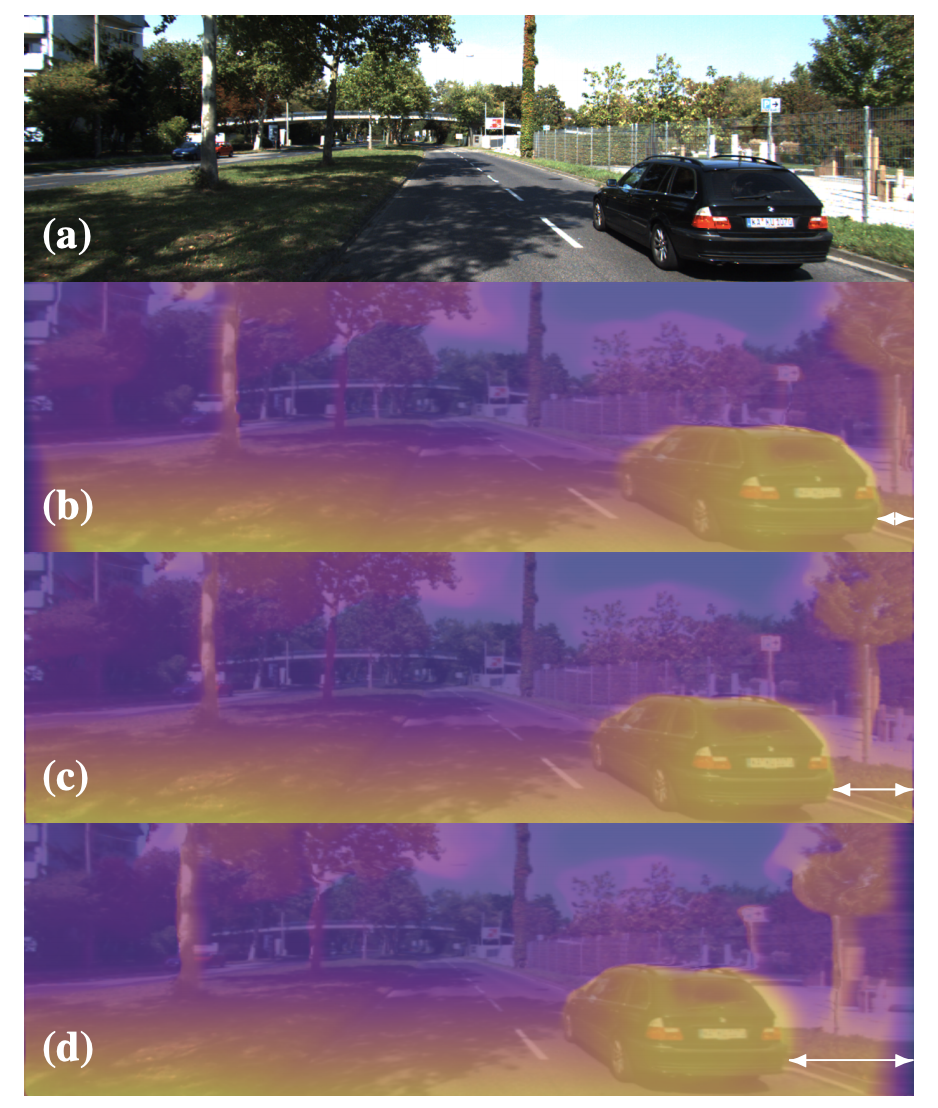
\includegraphics[width=0.5\linewidth]{Figures/SOA/illupoggi}
	\caption[Poggi et al. quanlitative evaluation.]{Poggi et al. quanlitative evaluation. a) is the input image, b) and d) are respectively the left and right estimation while c) is the center (image-aligned) estimation.}
	\label{illupoggi}
\end{figure}


This approach is mainly inspired by the different drawbacks of the previously mentioned methods. Indeed, the stereo systems suffer from the same constraints as the acquisition system. Occlusion, object boundaries and left image borders represent a significant challenge for these algorithms. Counteracting, \cite{poggi2018learning} proposes to emulate two views using the input as central image instead of one (for the stereo setup). As shown in Figure \ref{illupoggi}, the effect of such a procedure is, in addition to improving the accuracy, to eliminate the defects of the stereo system.


Many defects are present due to the use of a stereo based training procedure. Some have been reported like inconsideration of the occlusion or erroneous estimates due to second view hallucination.
In spite of this, these methods have reported results that have successively become references in the field. However, one factor remains crucial: the data. The chief drawback of such methods remains the training requirements. The use of an image pair, in addition to introducing constraints, is heavy and not necessarily available. Also, the necessary acquisition system is necessarily more constraining.
This is one of the major reasons why other methods requiring only one camera have been developed. Thus, the core concept of monocular estimation is no longer limited to the inference process but also to the training process.

\textbf{Self-supervised monocular-based. }Now that different stereo-based methods have been discussed, it is possible to shift towards monocular approaches which are nevertheless increasingly widespread.
Indeed, the fundamental interest of such an approach remains the training with a single camera. Taking advantage of the use of the temporal dimension, these techniques are based on principles similar to depth estimation by pure image processing by considering the displacement between cameras to infer a disparity. 

As a first outstanding contribution, \cite{zhou2017unsupervised} proposed to exploit the displacement between two successive images to infer depth. 

\begin{figure}[h]
	\centering
	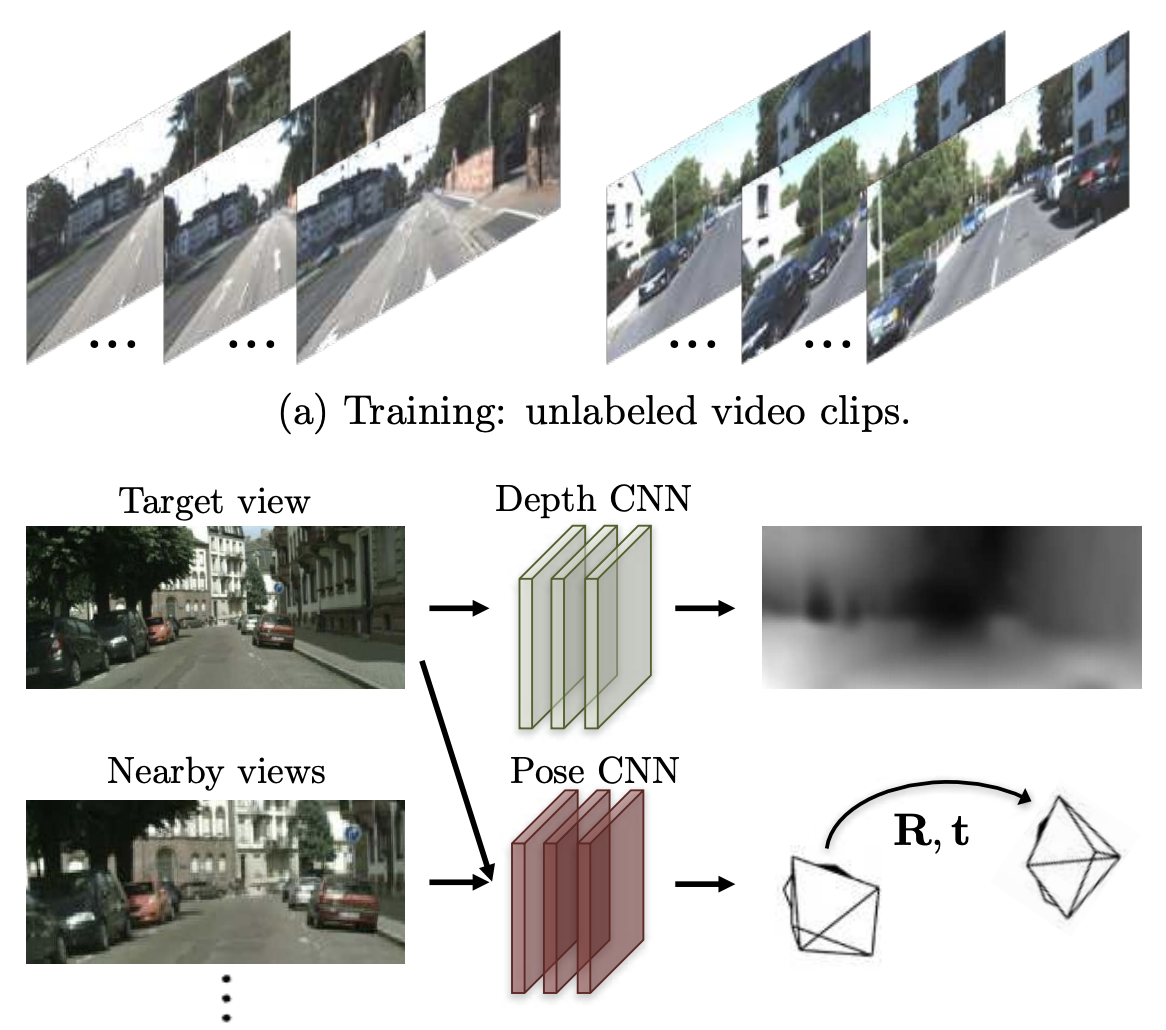
\includegraphics[width=0.5\linewidth]{Figures/SOA/illuzhou2017}
	\caption[Zhou et al. Architecture.]{Zhou et al.\cite{zhou2017unsupervised} Architecture.}
	\label{illuzhou2017}
\end{figure}

As shown in Figure \ref{illuzhou2017}, they allowed an advance towards a unified framework composed of two networks. One network estimates the depth from a first view at time $t$. A second network then tries to determine the displacement between this first view $I_t$ and a second one at time $t+1$ denoted $I_{t+1}$. Thus, similar to the no-learning-involved approach, this displacement $\{R,t\}$ allows the inverse deformation of the secondary image(s). Since a depth map and a camera pose are estimated, it is possible to project an image $I_{t+1}$ on the source view $I_{t}$. Thus, this deformation allows computing a photometric error between the projected views and the target image. Zhou et al. also emphasized some limitations of these architectures and proposed a set of overcomes. They determine a recurrent and problematic situation is the low-texture regions. Their solution is then based on approaches making the same observation (e.g. \cite{garg2016unsupervised},\cite{godard2017unsupervised}). They then propose to use an explicit multi-scale approach by forcing it directly into the network. Then, they explain in the cost function a weighted smoothing term. From these two actions, the gradient errors emanating from textureless regions are reduced and allow a perennial optimization. \cite{zhou2017unsupervised} also define a set of rules that allow the definition of operating cases.Thus, they determine that the scene must not present any moving object, not compoter any (dis)occlusion and observing only Lambertian surfaces. These three assumptions guarantee a sane gradient. 
These rules are critical since these problems will either be addressed in the next contributions described below or in the manuscript presented here.


In the same year, Yang et al. \cite{yang2017unsupervised} propose a \emph{edge-aware} approach. Contrary to a large majority of approaches, they decide to use normals which are a derivative of the depth. They claim this step allows a more geometrically faithful reconstruction. To integrate this concept, this contribution integrates layers specialized in this depth-to-normals conversion directly into the DCNN. As shown in Figure \ref{illuyang2017}, their architecture allows a bi-directional availability of the normal fields and thus to regularize with it.
This supplemental information can be derived from the depth implementing convolutions by considering the neighboring pixels.

\begin{figure}[h]
	\centering
	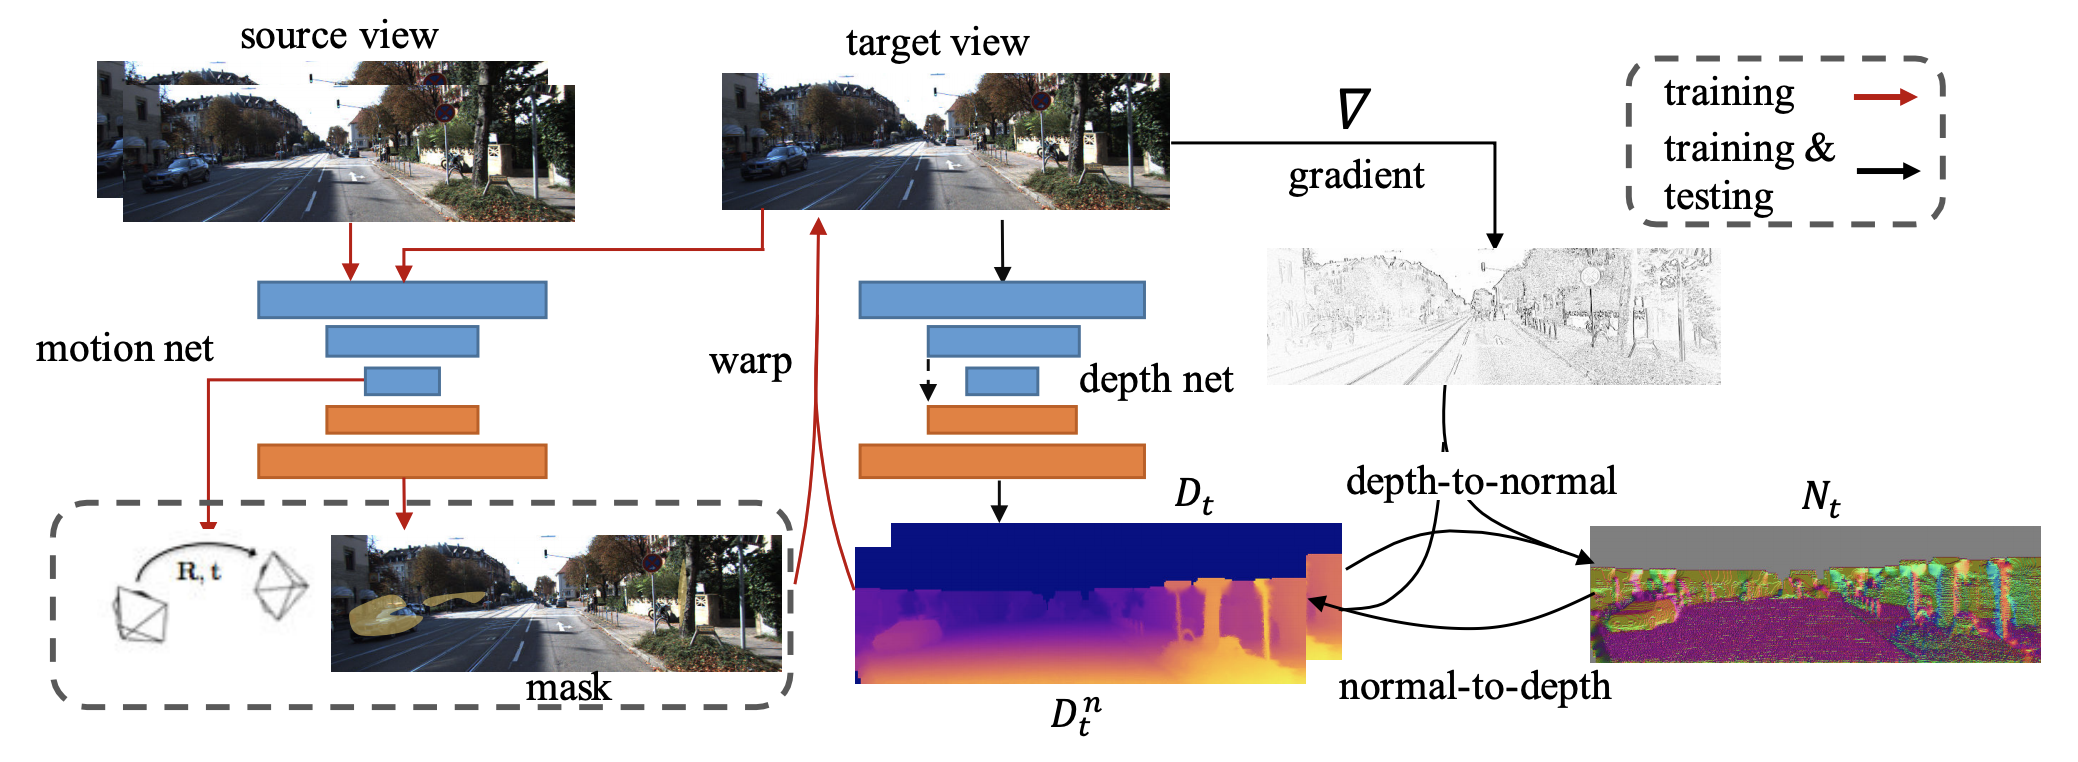
\includegraphics[width=0.8\linewidth]{Figures/SOA/illuyang2017}
	\caption[Framework propoed by Yang et al.]{Framework propoed by Yang et al.\cite{yang2017unsupervised}.}
	\label{illuyang2017}
\end{figure}


To come back briefly on the aspect \emph{edge-aware}, which constitute also a substantial part, they propose to modify the traditional smoothing function. Moreover, Yang et al. implement the use of the second order derivative allowing to eliminate ambiguities due to the surfaces but also to attempt reducing the bearing effect of the estimates.


In 2018, Mahjourian et al.\cite{mahjourian2018unsupervised} decide to focus on the geometric aspect by considering errors in 3D space. Thus, they operate a loss function composed of disciminant errors in two dimensions, 2D and 3D. 
This method also introduces a novel game-changing approach allowing to filter the areas of interest and to mask in an innovative way the out-of-bounds pixels to eliminate the remanent errors. In conclusion, their method considers a four-terms loss composed of a 3D cloud point alignment error, a 2D reconstruction error, a smoothing term and a dissimilarity measure.

\begin{figure}[h]
	\centering
	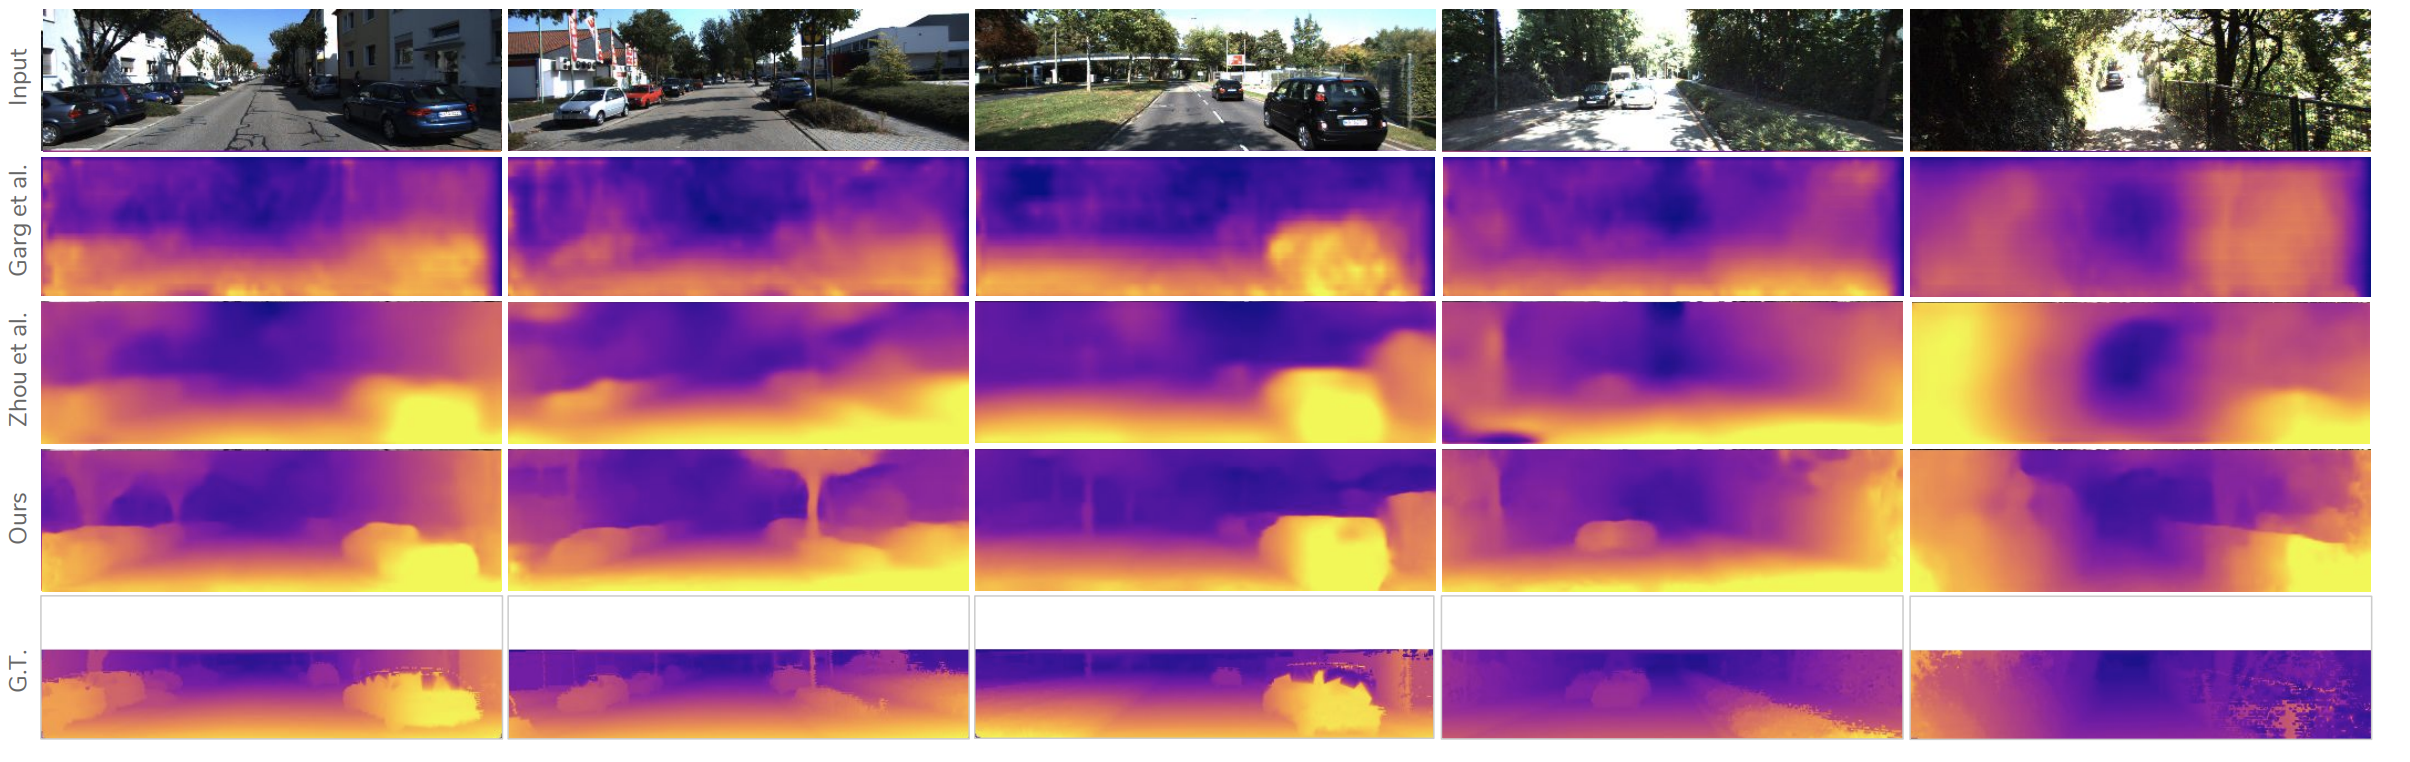
\includegraphics[width=0.8\linewidth]{Figures/SOA/mahjourian-illu}
	\caption[Mahjourian et al. Qualitative evaluation compared to previous methods..]{Mahjourian et al.\cite{mahjourian2018unsupervised} Qualitative evaluation compared to previous methods.}
	\label{mahjourian-illu}
\end{figure}


As shown in Figure \ref{mahjourian-illu}, their qualitative study highlights performance exceeding previous completions. \cite{mahjourian2018unsupervised} also demonstrates quantitatively, on the Kitti Eigen split benchmark, their performance is superior to previous approaches, despite a complexified loss.


The same year, GeoNet \cite{yin2018geonet} emerges and allows a triple estimation: the dense depth, the optical flow and the camera pose. To focus on the depth, the architecture named \emph{rigid structure reconstructor} is remarkably similar with the difference that they add a third block named \emph{non-rigid motion localizer} (see Figure \ref{geonet}).

\begin{figure}[h]
	\centering
	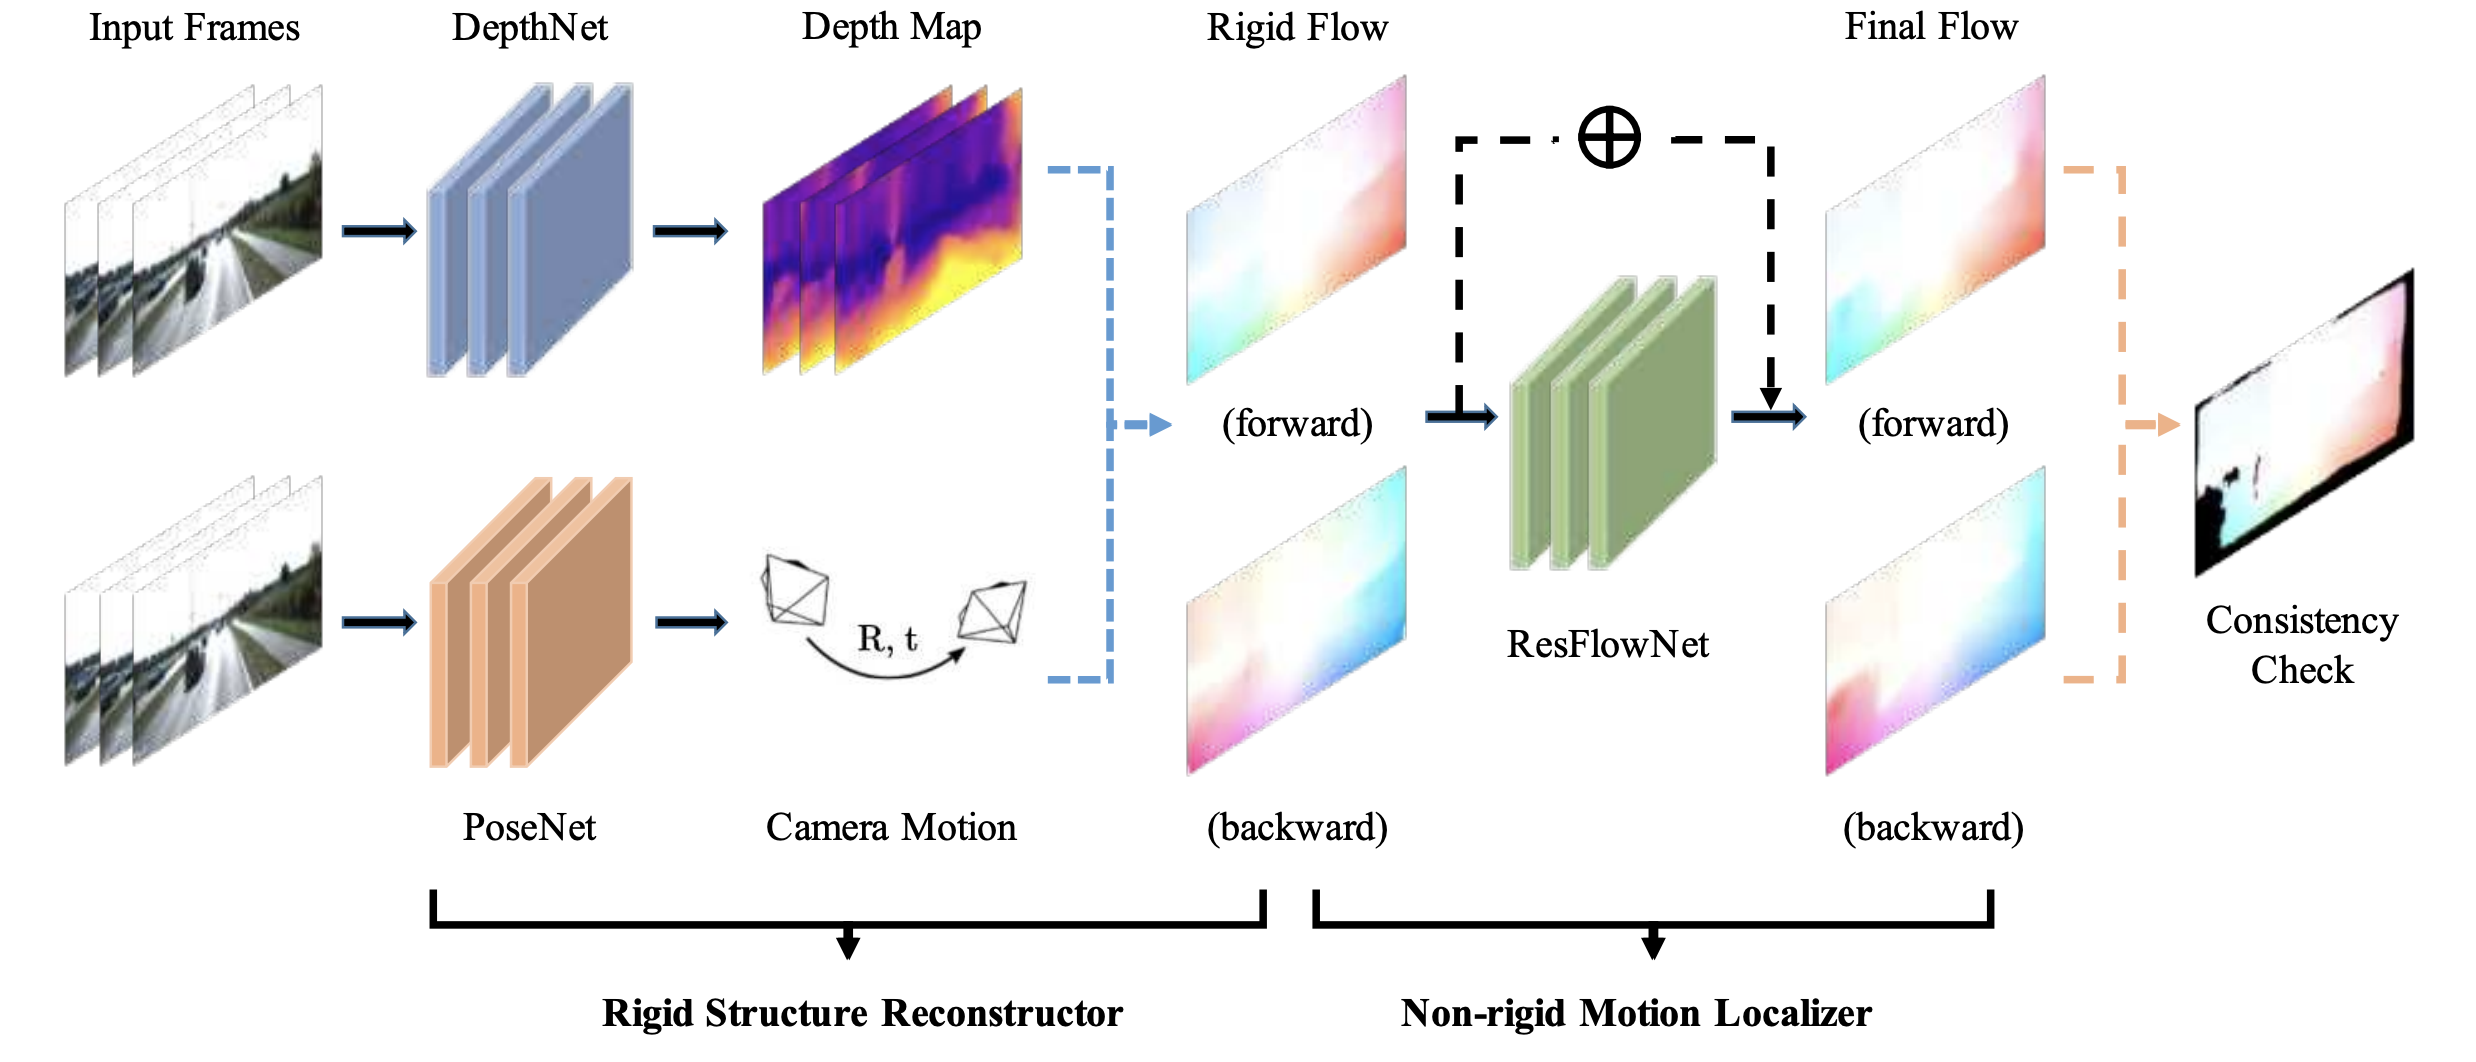
\includegraphics[width=0.8\linewidth]{Figures/SOA/geonet}
	\caption[Geonet Network.]{Geonet \cite{yin2018geonet} Network.}
	\label{geonet}
\end{figure}


Moreover, the authors attach a new importance to the choice of the loss terms and primarily consider two of the points stated by \cite{zhou2017unsupervised}. 
While their architecture \emph{rigid structure reconstructor} suffers from the same shortcomings as the previous approaches, the addition of this expansion and the associated loss allows to consider occlusion and non-Lambertian surfaces. Indeed, this part allows estimating a consistency measure which improves the robustness regarding these phenomena.


\cite{wang2018learning} proposes an originality by claiming that estimation does not necessarily require a learnable pose predictor. Indeed, this contribution proposes relying on the principles of \emph{direct visual odometry} (DVO) to eliminate this sub-architecture to estimate the displacement between two views.
Thus, the addition of a DVO \cite{steinbrucker2011real} pose predictor is used to replace the usual PoseCNN. Since it does not require training, it provides an established relationship between the estimated pose and the depth map. Moreover, this addition does not require any increased effort since it can be derived directly from the reconstructed image which equally serves as a discriminant for the DCNN. This proof of concept opened up the field of possibilities by outlining the possibility to eliminate blocks deemed essential while obtaining precise performance. 


Very similar to GeoNet\cite{yin2018geonet}, \cite{zou2018df} proposes an approach of joint estimation of depth and optical flow. The approach is slightly distinct since the architecture is drastically different. As shown in Figure \ref{illuzhou2018}, where GeoNet requires only two dissociable pipelines, DF-Net requires four. To summarize, as traditionally, a map is generated using a PoseCNN and auto-encoders allowing the evaluation of a depth consistency loss. In a second estimation pipeline, the pose estimate and the two estimated maps are aggregated to derive two maps respectively forward flow and backward flow. Ultimately, a flow is estimated from the two initial views and these same two maps can be estimated using a FlowNet. Ultimately, flow maps are deduced from the region of interest masks.

\begin{figure}[h]
	\centering
	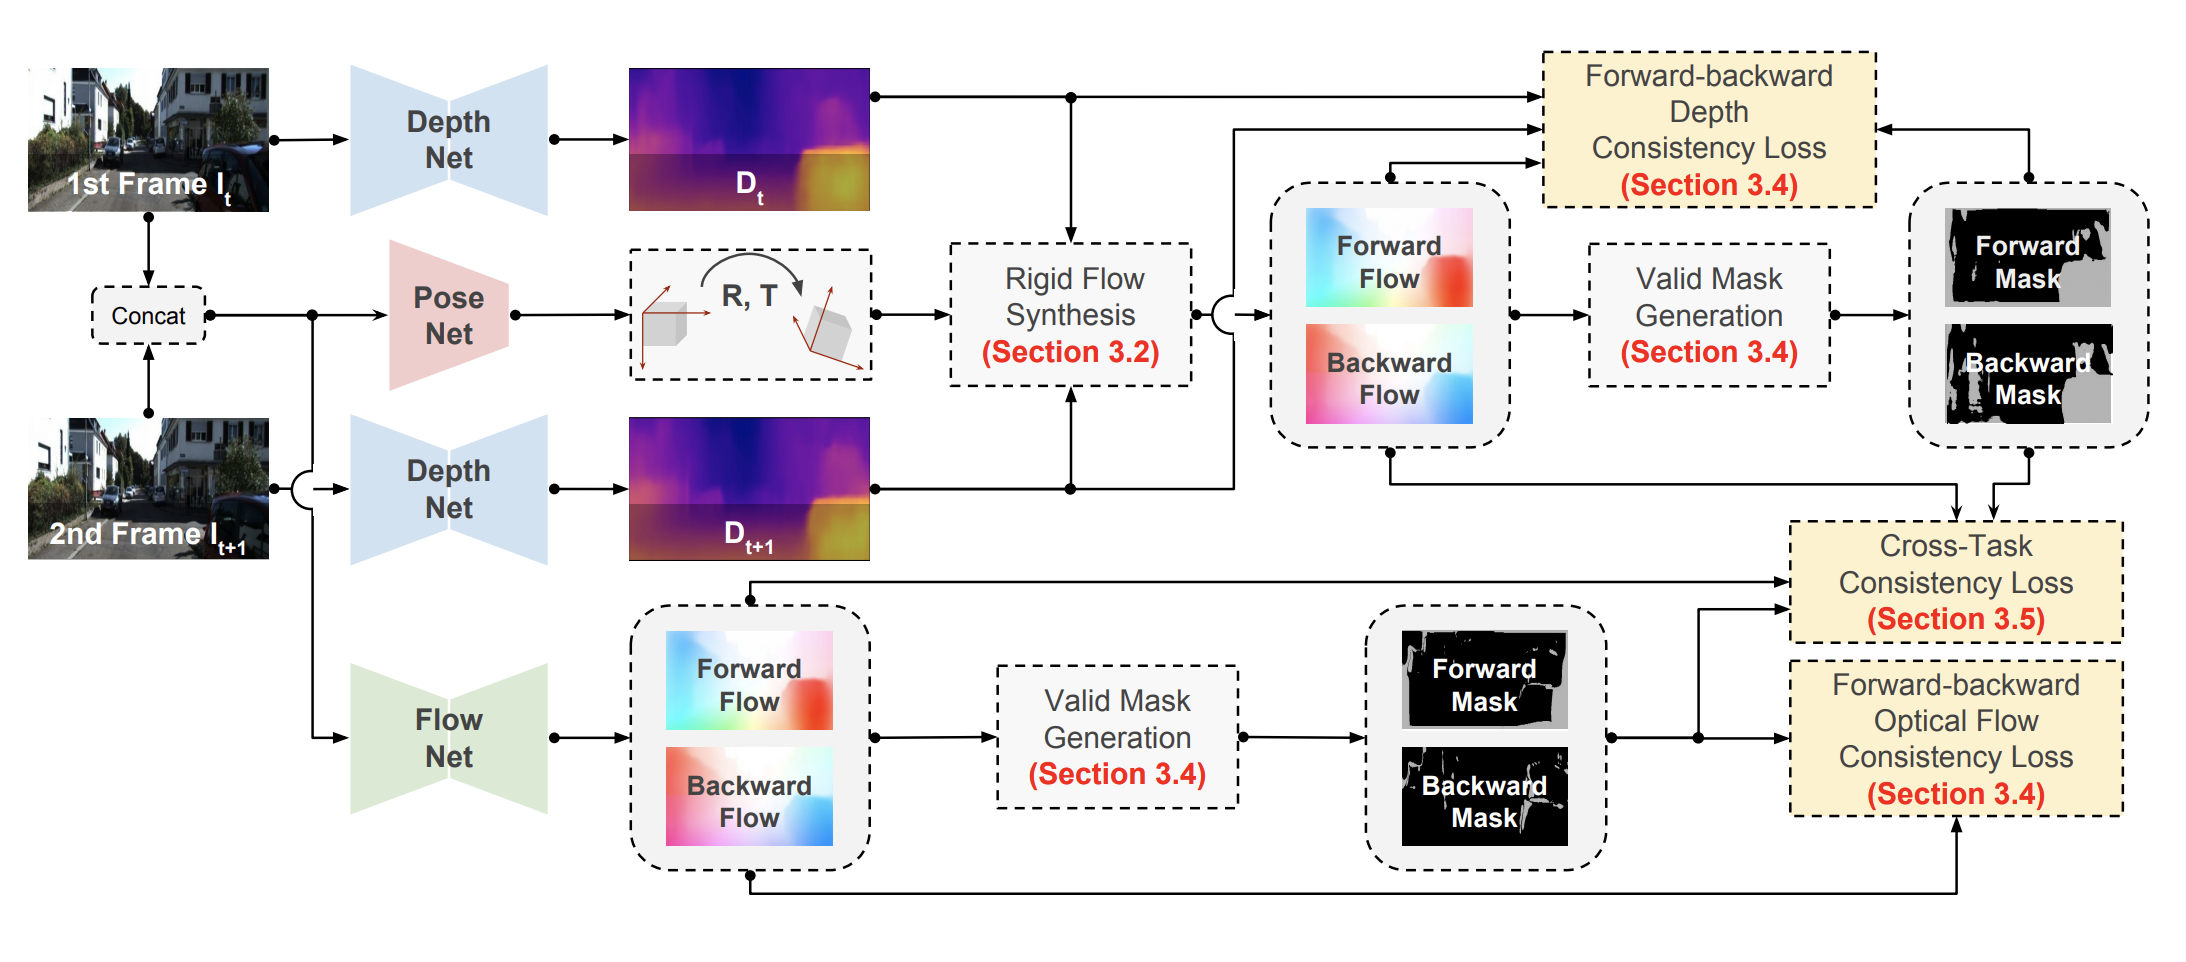
\includegraphics[width=0.8\linewidth]{Figures/SOA/illuzhou2018.png}
	\caption[DF-Net Architecture.]{DF-Net \cite{zou2018df} Architecture.}
	\label{illuzhou2018}
\end{figure}

 
All this information can be combined and compared using different terms. The \emph{Forward-backward Depth Consistency Loss} is used to ensure the consistency of forward and backward estimates. A smoothing term imposes smooth transitions while preserving the object boundaries. A photometric error is based on the assumption of brightness constancy and allows an evaluation between initial view and projection. And finally, \emph{Cross-task consistency} discriminates the differences between the optical flows estimated from the so-called rigid depth maps, and those estimated by the FlowNet. 
This method, with all the tools deployed, allows to jointly and precisely estimate a refined depth map and an optical flow. On the other hand, it is considerable the method described here represent a complicated version of GeoNet. However, the \textbf{Evaluation} sub-part will demonstrate Zou et al.'s method is slightly more efficient in estimating a depth map.


Yang et al. \cite{yang2018lego} promoted the principle of edge learning with their method called LEGO. It is based on the observation that any planar surface does not have edges until they are at the boundary of it which is similar to image processing based approaches. This allows them to define surfaces based on the absence of visual cues - here the edges -. As a consequence, it is possible to force the normals to follow the same direction for a defined surface. Based on this concept, this contribution observes a similar architecture, in two blocks, one for the depth and the other for the pose, and adds a third decoder dedicated to the edges.
Thus, employing their priors, the loss becomes a four-term minimizable function using in turn the boundary map, the depth map and the \emph{fly-out mask} allowing to eliminate the pixels not remaining in the target view due to the displacement between acquisitions. An illustration of their architecture is available below in Figure \ref{yang2018illu}.

\begin{figure}[h]
	\centering
	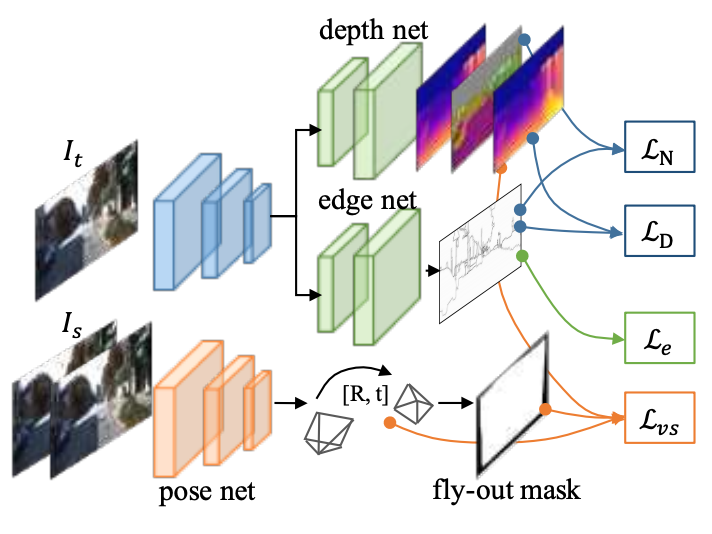
\includegraphics[width=0.4\linewidth]{Figures/SOA/yang2018illu}
	\caption[LEGO Architecture.]{LEGO Architecture \cite{yang2018lego}.}
	\label{yang2018illu}
\end{figure}


In 2019, Ranjan et al. \cite{ranjan2019competitive} propose joint learning of four descriptive images: depth, optical flow, camera motion and motion segmentation. The principal interest of this method lies in the first remarkable use of Counting Collaboration. Like so, this framework allows the joint learning of several collaborative networks in a coordinated manner. This organization is ruled by a discrimination system on the pixels according to their displacement. This core allows an explicit differentiation between moving and static surfaces deriving all previously named descriptive images in a transparent way. The authors define a training procedure including two major steps, competition and collaboration. This ultimately allows them to obtain robust results but also to generate unique descriptive images as the combination of segmented flow in the moving regions and optical flow. 


Following with another optical flow computation based approach, EPC++ \cite{luo2019every} is an extensively competitive network since it allows many current methods to compare to a very efficient network. The method starts from the fact that considering static scenes (as previously formulated) is unnecessary if we consider a network can understand the geometry of the scene as a whole. Thus, the authors propose learning jointly the 3D geometry per pixel and the motion. 

\begin{figure}[h]
	\centering
	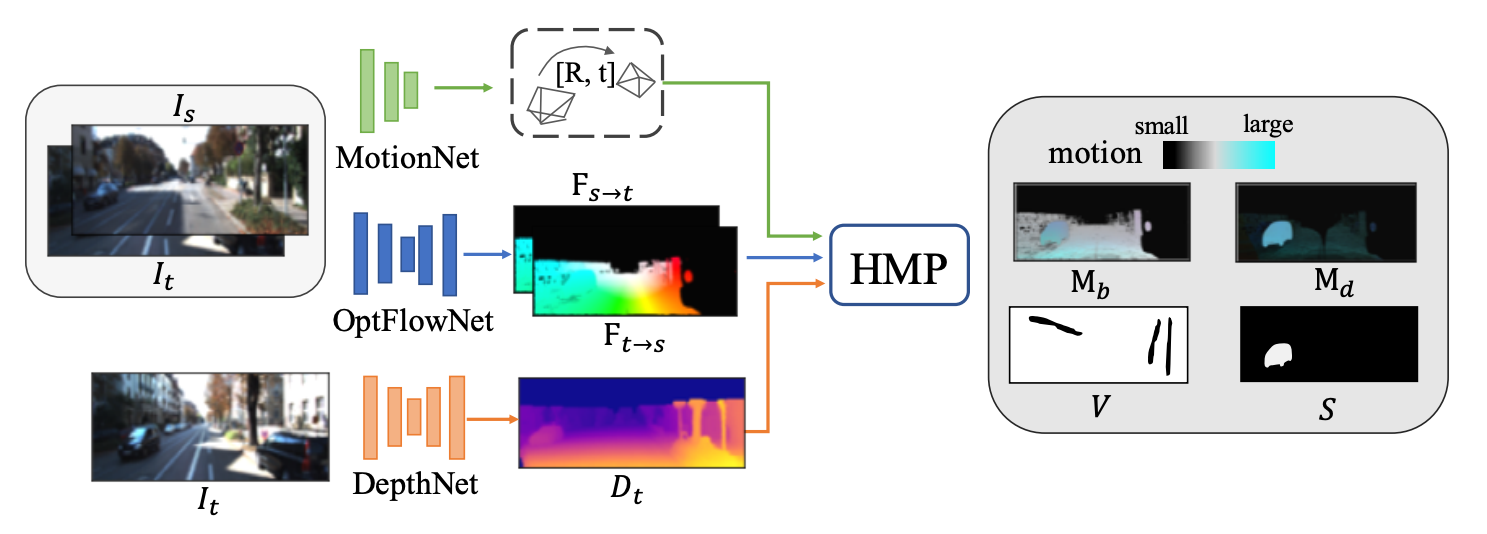
\includegraphics[width=0.8\linewidth]{Figures/SOA/illuepc++}
	\caption[EPC++ Architecture.]{EPC++ Architecture \cite{luo2019every}.}
	\label{illuepc}
\end{figure}


As shown in Figure \ref{illuepc}, this contribution opts for the use of three parallel networks each with a specific and differentiable task. A MotionNet encoder deduces the pose and two auto-encoders estimate the depth and the optical flow respectively. These three pieces of information, once given to what the authors designate an \emph{Holistic 3D Motion Parser}, allow to compute a segmentation mask for moving objects, an occlusion mask, and two 3D motion maps, one for the background, the other for the moving objects. This modeling allows to regress a precise depth map. Luo et al. also prove a network can learn to understand 3D motion at the pixel level, which emphasizes a high level of knowledge. The displayed performances show that a 3D geometry and motion concepts infused networks outperforms all previous methods.


In the same year as Luo et al. \cite{luo2019every}, Casser et al. \cite{casser2019depth} proposed a method with an original feature.This concept is based on a question: "What if 3D motion was modeled and used to refine a network on the fly? ". This method is motivated by the use of such estimators in an autonomous system. The authors subsequently propose adapting the estimation model in operation.

This contribution is based on the same setup as the significant contributions discussed above. An image sequence is used to retrieve the depth by means of the pose and deformation of consecutive images. In addition, they model a 3D motion object predictor based on the same architecture as the ego-motion predictor. Using an instance segmentation mask, Casser et al. propose to learn on-the-fly the prediction of this instance motion in 3D space. Addressing the recurrent problem of objects changing scale over time, the authors propose to allow the model to learn this phenomenon, thus avoiding the estimation errors involved. At long last, the pipeline learns on its own over time using short-training strategies on small sequences, hence reducing the discontinuity errors derived from the single-frame estimation. By this strategy, the model is refined as it observes more scenes. As shown in Figure \ref{casserillu}, this tactic allows, despite a shallower/less complex ensemble, to obtain qualitative results. Moreover, the learning complexity is reduced while making the system widely usable as an autonomous system. 

\begin{figure}[h]
	\centering
	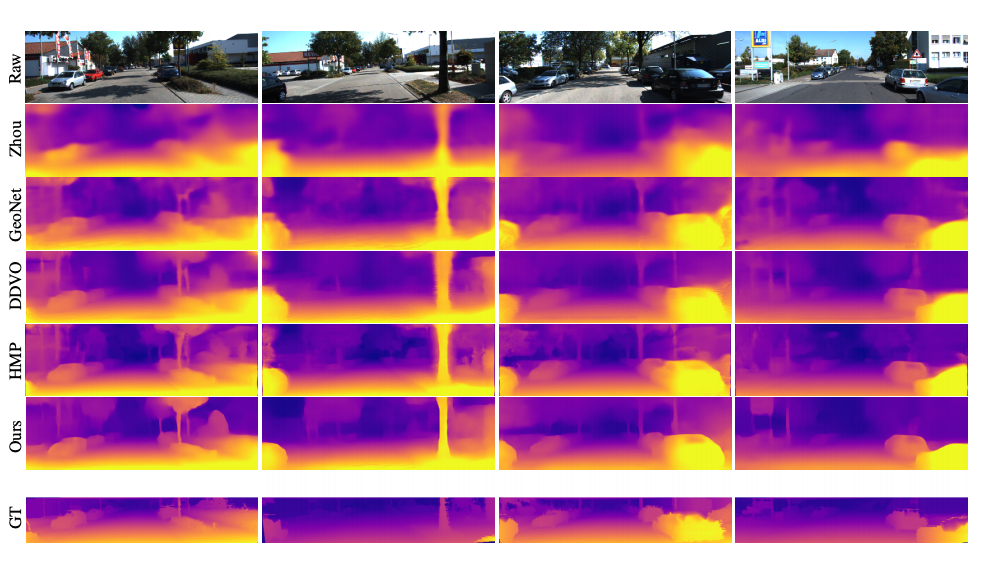
\includegraphics[width=0.8\linewidth]{Figures/SOA/casserillu}
	\caption[Quantitative evaluation of Casser et al. method.]{Quantitative evaluation of Casser et al. \cite{casser2019depth} method.}
	\label{casserillu}
\end{figure}


Neglecting this online approach, Monodepth v2 \cite{godard2019digging} is one of the best-known contributions of the community in this field. In fact, it represents, even today, the state-of-the-art in terms of robust depth map estimation. Godard et al. had in the past proposed an outstanding contribution that allowed a great advance. However, this previous method suffered from multiple flaws, one of which was the erroneous consideration of the occlusion. In reaction, the authors proposed Monodepth2, an increment of Monodepth v1.
This approach introduces three game-changer concepts:
\begin{itemize}
	\item A new design of reprojection loss to consider occlusion (\textit{Reprojection})
	\item A promising multi-scale UNet-based architecture  (\textit{Architecture})
	\item A masking strategy removing camera motion-related errors (\textit{Mask})
\end{itemize}

Embedding a dissimilarity measure and a L1 distance, the \textit{Reprojection} compare the target view with the warped second view. Although this approach is extremely similar to previouses, a \textit{Mask} is computed allowing the neglect of static pixels. As a considerable difference, while previous methods involved either optical flow or motion computation, this strategy consists solely into a per-pixel comparison of \textit{Reprojections} computed with different setups. Indeed, the \textit{Mask} is based on pixel-wise minimal photometric error between the target image and either the warped or the original second view.
Ultimately, Godard et al. proposed to benefit from UNet \cite{ronneberger2015u} skip connections as such \textit{Architecture} allow for seamless multi-scale computation. Indeed, the authors proposed to extract depth maps at intermediate layers and upsample those. Ultimately, this loss aggregation and computation at full resolution reduce texture-copy artifacts. The upsampling strategy prior to error computation enforces a correct full resolution reconstruction and avoids "holes" in the maps as usually seen in other multi-scale methods.
In Figure \ref{godardillu}, a schematic detailing the key principles is displayed.

\begin{figure}[h]
	\centering
	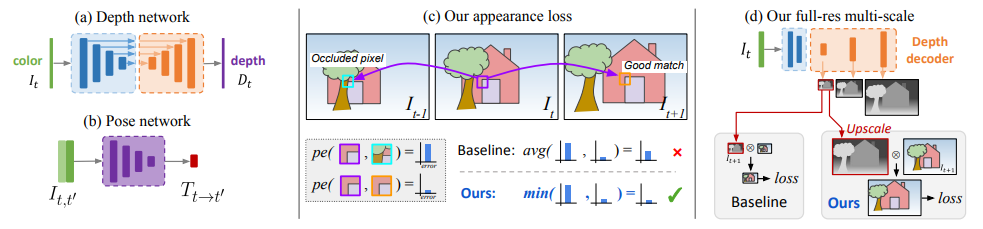
\includegraphics[width=0.8\linewidth]{Figures/SOA/godardillu}
	\caption[Monodepth v2 key principles.]{Monodepth v2 \cite{godard2019digging} key principles.}
	\label{godardillu}
\end{figure}

This approach was compared to all the methods previously explained. It clearly appears to be the most efficient, despite its reduced complexity. An absolutely remarkable fact in this contribution is the highlighting that the most important thing in a network is the objective function, especially in the self-supervised domain. Thus, a "simple" UNet can outperform other more dense methods by purely handling a properly dimensioned loss. Godard et al. have also proposed a method involving only two networks and requiring neither optical flow nor 3D motion. 
For all these reasons, this network remains the leading competitor in the race towards an accurate depth map. Therefore, this contribution will be used as a basis and benchmark for the methods developed for this manuscript. These methods will be explained in Chapter \ref{Chapter5}.



Very recently, Yang et al \cite{yang2020d3vo} proposed D3VO, an approach for joint learning of depth, pose and relative incertitude.


As improvement, some methods propose refining the depth map such as \cite{weder2020routedfusion} with RoutedFusion, or to define a depth-related uncertainty \cite{poggi2020uncertainty}.
Furthermore, some methods mobilize other further information to deduce the depth. Furthermore, many other features like semantics \cite{chen2019towards} or structured light pattern \cite{riegler2019connecting} seem to improve the estimation on an ad-hoc basis.




\textbf{Quantitative Evaluation.} This subpart proposes Table \ref{tab:evalsoadepth} to compare the different methods explained earlier. All methods have been evaluated on the Eigen Benchmark from KITTI dataset \cite{Geiger2012CVPR}.

% Please add the following required packages to your document preamble:
% \usepackage{graphicx}
\renewcommand{\arraystretch}{1.2}
\useunder{\uline}{\ul}{}
\begin{table}[h]
	\centering
	\caption[Quantitative evaluation. Comparison of depth estimation methods on KITTI 2015 the Eigen split.]{Quantitative evaluation. Comparison of depth estimation method to on KITTI 2015 \cite{Geiger2012CVPR} the Eigen split. Best results in each category are in \textbf{bold}; second best are \underline{underlined}. D is for depth supervision, D$^*$ for auxiliary depth supervision. S and M corresponds respectively to stereo and mono self-supervision.}
	\label{tab:evalsoadepth}
	\resizebox{\textwidth}{!}{%
		\begin{tabular}{lcccccccccc}
			&         &  & Abs Rel     & Sq Rel      & RMSE   & RMSE log &  & 1.25  & 1.25        & 1.25           \\ \cline{4-7} \cline{9-11} 
			Approach &
			Train &
			&
			\multicolumn{4}{c}{lower is better} &
			&
			\multicolumn{3}{c}{higher is better} \\ \hline
			Eigen \cite{eigen2014depth}                      & D       &  & 0.203       & 1.548       & 6.307  & 0.282    &  & 0.702 & 0.890       & 0.890          \\
			Liu \cite{liu2015learning}                       & D       &  & 0.201       & 1.584       & 6.471  & 0.273    &  & 0.680 & 0.898       & 0.967          \\
			Klodt \cite{klodt2018supervising}                     & D$^*$M  &  & 0.166       & 1.490       & 5.9998 & -        &  & 0.778 & 0.919       & 0.966          \\
			AdaDepth \cite{kundu2018adadepth}                  & D$^*$   &  & 0.167       & 1.257       & 5.578  & 0.237    &  & 0.771 & 0.922       & 0.971          \\
			Kuznietsov \cite{kuznietsov2017semi}                & DS      &  & 0.113       & 0.741       & 4.621  & 0.189    &  & 0.862 & 0.960       & 0.986          \\
			DVSO \cite{yang2018deep}                      & D$^*$S  &  & 0.097       & 0.734       & 4.442  & 0.187    &  & 0.888 & 0.958       & 0.980          \\
			SVSM FT \cite{luo2018single}                   & DS      &  & {\ul 0.094} & {\ul 0.626} & 4.525  & 0.177    &  & 0.891 & 0.965       & 0.984          \\
			{\underline{Guo} \cite{guo2018learning}} &
			DS &
			&
			0.096 &
			0.641 &
			{\ul 4.095} &
			{\ul 0.168} &
			{\ul } &
			{\ul 0.892} &
			{\ul 0.967} &
			{\ul 0.986} \\
			\textbf{DORN} \cite{fu2018deep} &
			D &
			&
			\textbf{0.072} &
			\textbf{0.307} &
			\textbf{2.727} &
			\textbf{0.120} &
			\textbf{} &
			\textbf{0.932} &
			\textbf{0.984} &
			\textbf{0.994} \\ \hline
			Zhou \cite{zhou2017unsupervised}                      & M       &  & 0.183       & 1.595       & 6.709  & 0.270    &  & 0.734 & 0.902       & 0.959          \\
			Yang \cite{yang2017unsupervised}                      & M       &  & 0.182       & 1.481       & 6.501  & 0.267    &  & 0.725 & 0.906       & 0.963          \\
			Mahjourian \cite{mahjourian2018unsupervised}                & M       &  & 0.163       & 1.240       & 6.220  & 0.250    &  & 0.762 & 0.916       & 0.968          \\
			GeoNet \cite{yin2018geonet}                     & M       &  & 0.149       & 1.060       & 5.567  & 0.226    &  & 0.796 & 0.935       & 0.975          \\
			DDVO \cite{wang2018learning}                      & M       &  & 0.151       & 1.257       & 5.583  & 0.228    &  & 0.810 & 0.936       & 0.974          \\
			DF-Net \cite{zou2018df}                    & M       &  & 0.150       & 1.124       & 5.507  & 0.223    &  & 0.806 & 0.933       & 0.973          \\
			LEGO \cite{yang2018lego}                      & M       &  & 0.162       & 1.352       & 6.276  & 0.252    &  & -     & -           & -              \\
			Ranjan \cite{ranjan2019competitive}                    & M       &  & 0.148       & 1.149       & 5.464  & 0.226    &  & 0.815 & 0.935       & 0.973          \\
			EPC++ \cite{luo2019every}                     & M       &  & 0.141       & 1.029       & 5.350  & 0.216    &  & 0.816 & 0.941       & 0.976          \\
			Struct2depth \cite{casser2019depth}              & M       &  & 0.141       & {\ul 1.026} & 5.291  & 0.215    &  & 0.816 & 0.945       & {\ul 0.979}    \\
			{\underline{Monodepth2 w/o pretraining} \cite{godard2019digging}} &
			M &
			&
			{\ul 0.132} &
			1.044 &
			{\ul 5.142} &
			{\ul 0.210} &
			&
			{\ul 0.845} &
			{\ul 0.948} &
			0.977 \\
			\textbf{Monodepth2 \cite{godard2019digging}} &
			M &
			&
			\textbf{0.115} &
			\textbf{0.903} &
			\textbf{4.863} &
			\textbf{0.193} &
			\textbf{} &
			\textbf{0.877} &
			\textbf{0.959} &
			\textbf{0.981} \\ \hline
			\textbf{Monodepth2 (1024 x 320) \cite{godard2019digging}} &
			M &
			&
			\textbf{0.115} &
			\textbf{0.882} &
			\textbf{4.701} &
			\textbf{0.190} &
			\textbf{} &
			\textbf{0.879} &
			\textbf{0.961} &
			\textbf{0.982} \\ \hline
			Garg \cite{garg2016unsupervised}                      & S       &  & 0.152       & 1.226       & 5.849  & 0.246    &  & 0.784 & 0.921       & 0.967          \\
			Monodepth R50 \cite{godard2017unsupervised}             & S       &  & 0.133       & 1.142       & 5.533  & 0.230    &  & 0.830 & 0.936       & 0.970          \\
			StrAT \cite{mehta2018structured}                     & S       &  & 0.128       & 1.019       & 5.403  & 0.227    &  & 0.827 & 0.935       & 0.970          \\
			3Net (R50) \cite{poggi2018learning}                & S       &  & 0.129       & 0.996       & 5.281  & 0.223    &  & 0.831 & 0.939       & 0.974          \\
			3Net (VGG) \cite{poggi2018learning}                & S       &  & 0.119       & 1.201       & 5.888  & 0.208    &  & 0.844 & 0.941       & \textbf{0.978} \\
			{\underline{SuperDepth (1024 x 382)} \cite{pillai2019superdepth}} &
			S &
			&
			{\ul 0.112} &
			{\ul 0.875} &
			\textbf{4.958} &
			\textbf{0.207} &
			&
			{\ul 0.852} &
			{\ul 0.947} &
			{\ul 0.977} \\
			Monodepth2 w/o pretraining \cite{godard2019digging}& S       &  & 0.130       & 1.144       & 5.485  & 0.232    &  & 0.831 & 0.932       & 0.968          \\
			\textbf{Monodepth2} \cite{godard2019digging} &
			S &
			&
			\textbf{0.109} &
			\textbf{0.873} &
			{\ul 4.960} &
			{\ul 0.209} &
			&
			\textbf{0.864} &
			\textbf{0.948} &
			0.975 \\ \hline
			\textbf{Monodepth2 (1024 x 320)} \cite{godard2019digging} &
			S &
			&
			\textbf{0.107} &
			\textbf{0.849} &
			\textbf{4.764} &
			\textbf{0.201} &
			\textbf{} &
			\textbf{0.874} &
			\textbf{0.953} &
			{\ul 0.977} \\ \hline
			UnDeepVO \cite{li2018undeepvo}                  & MS      &  & 0.183       & 1.730       & 6.570  & 0.268    &  & -     & -           & -              \\
			Zhan FullNYU \cite{zhan2018unsupervised}              & D$^*$MS &  & 0.135       & 1.132       & 5.585  & 0.229    &  & 0.820 & 0.933       & 0.971          \\
			EPC++ \cite{luo2019every}                     & MS      &  & 0.128       & 0.935       & 5.0111 & 0.209    &  & 0.831 & 0.945       & \textbf{0.979} \\
			Monodepth2 w/o pretraining \cite{godard2019digging} & MS      &  & 0.127       & 1.031       & 5.266  & 0.221    &  & 0.836 & 0.943       & 0.974          \\
			\underline{Monodepth2} \cite{godard2019digging}                & MS      &  & 0.106       & 0.818       & 4.750  & 0.196    &  & 0.874 & {\ul 0.957} & \textbf{0.979} \\
			D3VO uncertainty \cite{yang2020d3vo} &
			MS &
			&
			{\ul 0.101} &
			{\ul 0.772} &
			{\ul 4.532} &
			{\ul 0.190} &
			&
			{\ul 0.884} &
			0.956 &
			{\ul 0.978} \\
			D3VO ablation \cite{yang2020d3vo}             & MS      &  & 0.105       & 0.791       & 4.650  & 0.193    &  & 0.878 & {\ul 0.957} & \textbf{0.979} \\
			\textbf{D3VO full} \cite{yang2020d3vo} &
			MS &
			&
			\textbf{0.099} &
			\textbf{0.763} &
			\textbf{4.485} &
			\textbf{0.185} &
			&
			\textbf{0.885} &
			\textbf{0.958} &
			\textbf{0.979} \\ \hline
			\textbf{Monodepth2 (1024 x 320)} \cite{godard2019digging} &
			MS &
			&
			\textbf{0.106} &
			\textbf{0.806} &
			\textbf{4.630} &
			\textbf{0.193} &
			\textbf{} &
			\textbf{0.876} &
			\textbf{0.958} &
			\textbf{0.980}
		\end{tabular}%
	}
\end{table}

\textbf{Summary and conclusions. } 

As it has been demonstrated, the scientific community attaches considerable importance to depth estimation. In recent years, researchers have turned to modern deep learning methods. Indeed, this allows less constrained approaches. Regrettably, the use of these techniques ordinarily requires strong assumptions but above all a massive amount of data. Moreover, it is notable that the models trained with certain data are linked to it, and consequently, when the modality used neglects certain phenomena, so do the models. 



 
% Chapter 1

\chapter{Preliminary} % Main chapter title

\label{Chapter3} % For referencing the chapter elsewhere, use \ref{Chapter1} 


This chapter is dedicated to the two main tools that will be widely used in this manuscript. To avoid redundancy and repetitive explanations, we propose defining Polarization in Section \ref{Polar_explain} and Deep Learning in Section \ref{DL_explain}. Thus, when general principles are needed for the understanding of the work, this chapter will serve as a reference.
%----------------------------------------------------------------------------------------

% Define some commands to keep the formatting separated from the content 


%----------------------------------------------------------------------------------------

\section{Polarimetry}\label{Polar_explain}

This section will be dedicated to polarimetry and will provide a general introduction to the field. We propose to describe this modality by defining it in three aspects. First, Section \ref{gdpola} introduce the general concept of polarization. Then, Section \ref{particularsensor} will take the sensor angle to discuss the properties specific to polarimetric imaging. Finally, in Section \ref{exploitdata}, we will discuss the usual exploitation methods of this particular data.


\subsection{General Principles}\label{gdpola}

Polarimetry \cite{collett2005field} is a particular modality that acquires the polarization state of objects in a scene. Briefly, polarization is a property that, in the case of image acquisition, concerns light. It is composed of two perpendicular fields called electric field $\vec{E}$ and magnetic field $\vec{B}$ that oscillate along the wave reflected to the sensor. A polarized wave is said to be elliptical but is ordinarily considered as the sum of linear and circular components.
In general, in mobile acquisition systems, only the linear polarization is acquired since the circular polarization requires the mounting of a quarter wave plate.
It is possible to observe polarized light in nature with sunlight or observation of multiple non-natural light sources. A notable property of polarization is that if a light wave hits a surface and is reflected, then the wave becomes partially polarized. This property is particularly important since, unlike conventional modalities that focus on colors or textures, polarimetry focuses on light behavior in relation to surfaces.

Consequently, it is possible to affirm that polarimetry allows the acquisition of changes in the state of light\cite{wolff1995polarization}. In addition, many principles are inspired or derived from Fresnel's equations \cite{fresnel1868oeuvres}. This link is attributed to the close relationship between polarization and reflection of light. Therefore, it is notable that polarization has the potential capacity to infer, by light behavior, the properties of surfaces (i.e. refractive index, surface normals, etc.).



\subsection{A Particular Sensor}\label{particularsensor}

The sensor allowing the acquisition of such data is particular.
Indeed, it could be compared to RGB if we consider the Bayer matrix. As shown in Figure \ref{fig:sensor}, a polarimetric camera has a microgrid of polarizers that allow the acquisition of polarization.

\begin{figure}[h]
	\centering
	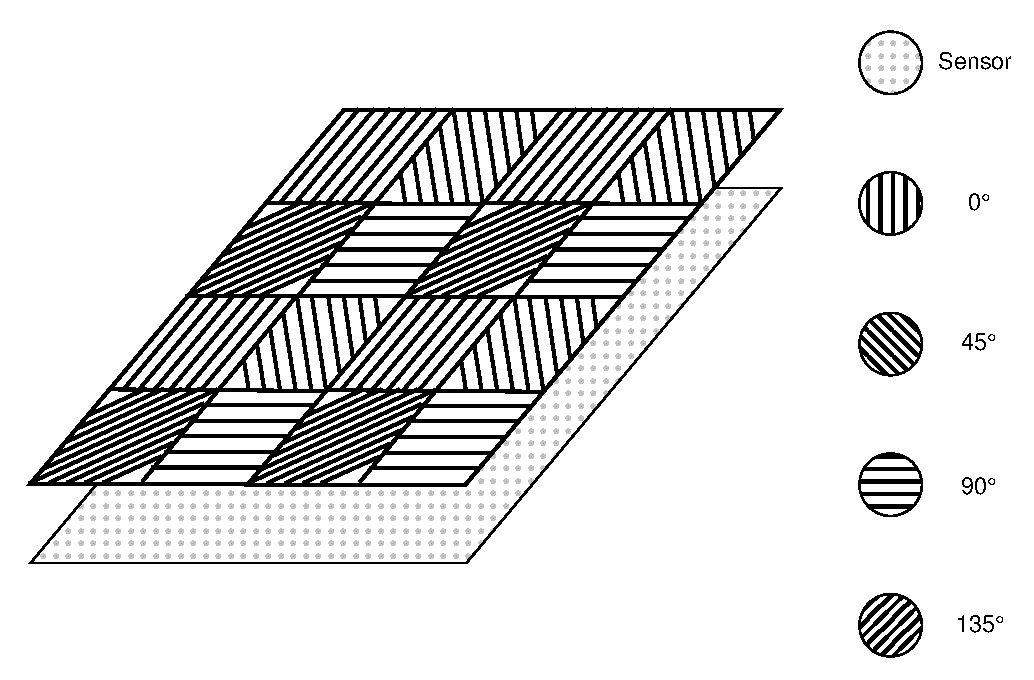
\includegraphics[width=0.8\linewidth]{Figures/Preliminary/sensor}
	\caption{Illustration of a DoFP polarization sensor micro-grid.}
	\label{fig:sensor}
\end{figure}

It is then possible to observe a multitude of mini polarizers with four different orientations affixed to the sensor. This technology is called Division of Focal Plane (DoFP).
Before the arrival of this technology, the cameras required a mechanical action to rotate the polarizers in front of the camera. Since then, with the DoFP, it is possible to acquire all the necessary information in a single shot. Hence, the sensors could be embedded to make dynamic acquisitions.
Standardly, there are four angles $\{0,45,90,135\}$ allowing calculations which will be discussed below.
These different angles allow discriminating the components of the light and thus to separate the waves. As schematized in Figure \ref{extract}, thanks to these different orientations, the light can be filtered.

\begin{figure}{h}
	\centering
	\colorlet{crystal}{gray}
	
	\def\zangle{-20}
	\def\xangle{20}
	
	\begin{tikzpicture}[x=(\xangle:0.75cm), y=(90:1cm), z=(\zangle:1.5cm),
	>=stealth, line cap=round, line join=round,
	lines/.style={gray!70, thick}, 
	axis/.style={black, thick},
	plate/.style={fill, opacity=0.875},
	markers/.style={darkgray!80, thick},
	markerss/.style={black!30, thick}]
	
	
	
	
	\begin{scope}[shift={(0,0,3.125)}]
	
	\node [yslant=tan(\zangle), above=0.25cm, align=center,font=\footnotesize] at 
	(1,1,1.5){Linearly Polarized Light};
	
	\begin{scope}[xscale=1.5, yscale=1.5]
	\path [crystal!25, plate] 
	(-1,-1,0) -- (-1,1,0) -- (1,1,0) -- (1,-1,0) -- cycle;
	\path [crystal!50, plate] 
	(-1,-1,0) -- (-1,-1,-0.125) -- (-1,1,-0.125) -- (-1,1, 0) -- cycle;
	\path [crystal!75, plate] 
	(-1,1,0) -- (-1,1,-0.125) -- (1,1,-0.125) -- (1,1, 0) -- cycle;
	\node [yslant=tan(\xangle), text=crystal!50, below, font=\small] at 
	(-1.125,-1,0){Sensor};
	\end{scope}
	
	
	\draw [markers] (0,1) -- (0,-1) (-0.5,0) -- (0.5,0);
	
	\draw [axis] (0,0,0) -- (0,0,3);
	
	\foreach \k [evaluate={%
		\i=\k*5.625; \j=\i>0 ? \i-5.625 : 0; 
		\a=90-\i; 
		\b=90-\j; 
		\c=int(mod(\k,4)==0 && sin \a != 0); 
		\d=int(\k+1/4);}] in {0,...,192}{
		\ifodd\d
		\ifnum\c=1
		\draw [->,opacity=0.3] (0,0,\i/360) -- ++(sin \a, sin \a, 0);
		\fi
		\draw [thick, red!80] (sin \a, sin \a, \i/360) -- (sin \b, sin \b, \j/360);
		\else
		\draw [thick, red!80] (sin \a, sin \a, \i/360) -- (sin \b, sin \b, \j/360);
		\ifnum\c=1
		\draw [->,opacity=0.3] (0,0,\i/360) -- ++(sin \a, sin \a, 0);
		\fi
		\fi
	}
	\end{scope}
	
	\begin{scope}[shift={(0,0,6.125)}]
	
	\node [yslant=tan(\zangle), above=0.25cm, align=center,font=\footnotesize] at 
	(1,1,1.5){Unpolarized Light};
	
	\begin{scope}[xscale=1.5, yscale=1.5]
	\path [crystal!25, plate] 
	(-1,-1,0) -- (-1,1,0) -- (1,1,0) -- (1,-1, 0) -- cycle;
	\path [crystal!50, plate] 
	(-1,-1,0) -- (-1,-1,-0.0625) -- (-1,1,-0.0625) -- (-1,1, 0) -- 
	cycle;
	\path [crystal!75, plate] 
	(-1,1,0) -- (-1,1,-0.0625) -- (1,1,-0.0625) -- (1,1, 0) -- cycle;
	\node [yslant=tan(\xangle), text=crystal!50, below, font=\small] at 
	(-1,-1,0){45$^\circ$ Linear Polarizer};
	\end{scope}
	
	
	\draw [markerss] (-1.25,0.75) -- (-0.75,1.25);
	
	\draw [markerss] (-1.25,0.25) -- (-0.25,1.25);
	
	\draw [markerss] (-1.25,-0.25) -- (0.25,1.25);
	
	\draw [markerss] (-1.25,-0.75) -- (0.75,1.25);
	%up
	\draw [markerss] (-1.25,-1.25) -- (1.25,1.25);
	%down
	\draw [markerss] (-0.75,-1.25) -- (1.25,0.75);
	
	\draw [markerss] (-0.25,-1.25) -- (1.25,0.25);
	
	\draw [markerss] (0.25,-1.25) -- (1.25,-0.25);
	
	\draw [markerss] (0.75,-1.25) -- (1.25,-0.75);
	
	
	\foreach \k [evaluate={%
		\i=\k*5.625; \j=\i>0 ? \i-5.625 : 0; 
		\a=90-\i; 
		\b=90-\j; 
		\c=int(mod(\k,4)==0 && sin \a != 0); 
		\d=int(\k+1/4);}] in {0,...,192}{
		\ifodd\d
		\ifnum\c=1
		\draw [->,opacity=0.3] (0,0,\i/360) -- ++(sin \a, sin \a, 0);
		\fi
		\draw [thick,red!80] (sin \a, sin \a, \i/360) -- (sin \b, sin \b, \j/360);
		\else
		\draw [thick,red!80] (sin \a, sin \a, \i/360) -- (sin \b, sin \b, \j/360);
		\ifnum\c=1
		\draw [->,opacity=0.3] (0,0,\i/360) -- ++(sin \a, sin \a, 0);
		\fi
		\fi
	}
	
	\foreach \k [evaluate={%
		\i=\k*5.625; \j=\i>0 ? \i-5.625 : 0; 
		\a=90-\i; 
		\b=90-\j; 
		\c=int(mod(\k,4)==0 && cos \a != 0); 
		\d=int(\k+1/4);}] in {0,...,192}{
		\ifodd\d
		\ifnum\c=1
		\draw [->,opacity=0.3] (0,0,\i/360) -- ++(cos \a, 0, 0);
		\fi
		\draw [thick,teal] (cos \a, 0, \i/360) -- (cos \b, 0, \j/360);
		\else
		\draw [thick,teal] (cos \a, 0, \i/360) -- (cos \b, 0, \j/360);
		\ifnum\c=1
		\draw [->,opacity=0.3] (0,0,\i/360) -- ++(cos \a, 0, 0);
		\fi
		\fi
	}
	
	\foreach \k [evaluate={%
		\i=\k*5.625; \j=\i>0 ? \i-5.625 : 0; 
		\a=90-\i; 
		\b=90-\j; 
		\c=int(mod(\k,4)==0 && sin \a != 0); 
		\d=int(\k+1/4);}] in {0,...,192}{
		\ifodd\d
		\ifnum\c=1
		\draw [->,opacity=0.3] (0,0,\i/360) -- ++(0, sin \a, 0);
		\fi
		\draw [thick,orange] (0, sin \a, \i/360) -- (0, sin \b, \j/360);
		\else
		\draw [thick,orange] (0, sin \a, \i/360) -- (0, sin \b, \j/360);
		\ifnum\c=1
		\draw [->,opacity=0.3] (0,0,\i/360) -- ++(0, sin \a, 0);
		\fi
		\fi
	}
	
	\draw [ultra thick, ->] (0,0,3.5) -- (0,0,3);
	
	\end{scope}
	
	\end{tikzpicture}
	\caption{Illustration of unpolarized light filtration through $45\deg$ linear polarizer.}\label{extract}
\end{figure}


This filtering is reproduced with the different orientations of each micro-polarizer and thus allows the acquisition of a multitude of linearly polarized light components. 
Due to this sensor architecture, each pixel is independent since the information is influenced by the polarizer. Consequently, the images of each polarizer $P_{\{0,45,95,135\}}$ is "independent" and especially sparse. As shown in Figure \ref{fig:polaexplain}, it is possible to recognize the microgrid by zooming in on an image.

\begin{figure}[h]
	\centering
	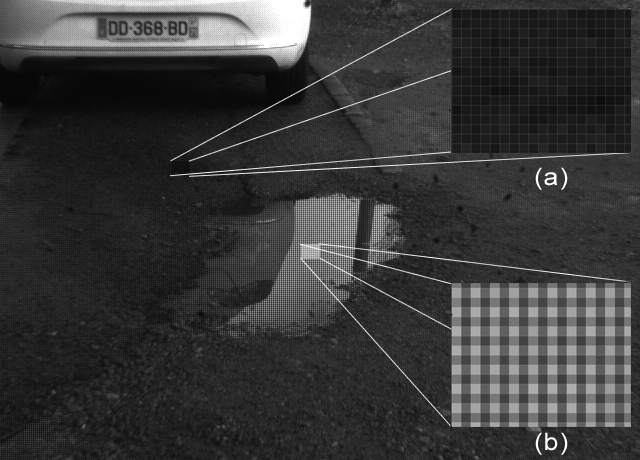
\includegraphics[width=0.6\linewidth]{Figures/VISAPP/polaexplain}
	\caption[Zoom on a polarimetric image.]{Zoom on a polarimetric image. (a) is a zoom on the non-polarized area, (b) is on a polarized area. Clearly, on a polarized surface, the micro-grid appear and reveal an intensity change according to the polarizer affected.}
	\label{fig:polaexplain}
\end{figure}

Subsequently, it is possible to identify polarized areas using this pixelization phenomenon. Indeed, when an object reflects the light, the grid appears since the intensities per polarizer are different (consequence of the filtering).


\subsection{Exploiting the Data}\label{exploitdata}


As previously stated, the images are sparse because of the sensor architecture. When the images are acquired with a low resolution sensor then this can cause a significant problem since the image size is divided by two. In addition, on a low resolution, the shapes can be changed because of the correspondence between the real world and image space. Ultimately, it is necessary that the polarizer images are dense and aligned otherwise the polarimetric information is incomplete.

To overcome this dimensionality problem, many approaches have been developed that allow the interpolation of polarimetric intensities. Principally used, Ratliff et al. \cite{ratliff2009interpolation} proposes to use a bilinear interpolation directly on the intensity images. More recently, more complex interpolation startegies have been investigated using the Newton polynomial \cite{li2019demosaicking} or the use of machine learning models based on sparse representation \cite{zhang2018sparse}.
Despite the complexity of these algorithms, the best way to overcome the image sparsity problem is to operate a high-resolution camera with smaller pixels and, above all, a more adequate real-world correspondence to image space.
The density of the polarization images is crucial to calculate the Stokes parameters \cite{stokes1851composition}.
These parameters have been designed to describe the polarization of light through a descriptive vector such as:

\begin{equation}
S = \begin{pmatrix}S_0\\S_1\\S_2\\S_3\end{pmatrix} = \begin{pmatrix}P_H + P_V\\ P_H - P_V\\ P_{45} - P_{135} \\ P_R - P_L\end{pmatrix} = \begin{pmatrix}P_0 + P_{90}\\ P_0 - P_{90}\\ P_{45} - P_{135} \\ 0\end{pmatrix} = \begin{pmatrix}I\\ Q\\ U \\ V\end{pmatrix},
\end{equation}

where $P_H$ and $P_V$ are respectively the horizontal and vertical polarization. Since we do not acquire circular polarization, $V$ and therefore $s_3$ remain null. $I$ represents the total acquired intensity whereas $U$ and $Q$ are part of $L = Q + iU$ the straight polarization intensity, being a complex number that accounts for the tilt of the polarization direction $\theta$.

\begin{figure}[h]
	\centering
	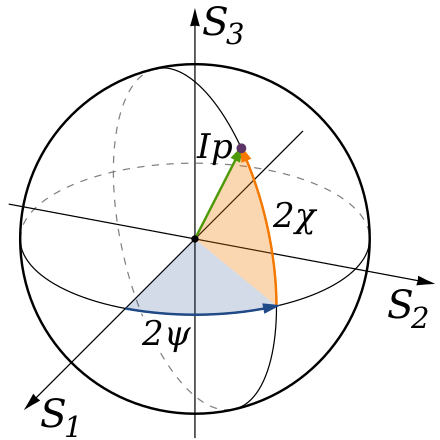
\includegraphics[width=0.3\linewidth]{Figures/Preliminary/pointcare}
	\caption{Spherical representation of Stokes vector on Poincar\'e Sphere.}
	\label{fig:pointcare}
\end{figure}

As stated in Section \ref{gdpola}, the polarization is said elliptical. Nevertheless, common representation projects the vector onto Poincar\'e sphere. Consequently, Stokes parameters can also be defined through 3 spherical coordinates $I_p$, $2\psi$ and $2\chi$ shown in Figure \ref{fig:pointcare}. Equally, the parameters are:

\begin{equation}
	\begin{cases}
	S_0 = I_p \\
	S_1 =  I_p \cos 2\psi \cos 2\chi\\
	S_2 =  I_p \sin 2\psi \cos 2\chi\\
	S_3 =  I_p \sin 2 \chi
	\end{cases},
\end{equation}

where $I_p$ is the intensity of the beam, $\psi$ and $\xi$ are defining factor for an ellipse being $\pi$ and $\frac{\pi}{2}$ invariant.
Consequently, one can define the intensity $\iota$, the angle of polarization $\alpha$ as well as the degree of polarization $\rho$ following (with no circular polarization acquired): 

\begin{equation}
\begin{cases}
\iota = S_0 =  I_p \\[8pt] 
\alpha = \frac{1}{2} \arctan \frac{S_2}{S_1}  = \psi\\[8pt] 
\rho =  \frac{\sqrt{S_1^2 + S_2^2}}{S_0}
\end{cases}.
\end{equation}

The degree $\rho$ and angle $\alpha$ of polarization are two very descriptive characteristics of polarization. $\rho$ is analogous to the polarization strength and belongs to $\left[0,1\right]$. This parameter quantify the polarization light in a wave. Therefore, a completly specular wave will record $\rho = 1$.

$\alpha \in \left[\frac{-\pi}{2}, \frac{\pi}{2}\right]$ is the angle of the electric field $\vec{E}$ projected on the image plane. In other words, the polarization angle corresponds to the orientation of the polarization with regard to the incident plane.

\subsection{Summary}

This section review the fundamental principles of polarization imaging. It showed how this modality is particular and requires a singular processing. In the same way, it is possible to realize that this information can be very useful for certain domains. Indeed, we have first stated the particularities of the acquisition of the polarization state of objects. This allowed us to establish a direct link between the surface and the light reflected by it. Next, we described the functioning of the sensors and their limits. To conclude, we have described general process making raw polarimetric images exploitable. This brief overview has, in addition to introducing the subject and establishing it, justified in large part the use of this particular information in our work.





\section{Deep Learning}\label{DL_explain}

This section will be dedicated to the main notions related to Deep Learning. The recent advances in the field of learning and the increase in computing power have allowed this sub-branch of machine learning to emerge. Moreover, the availability of data, which is crucial for this kind of greedy algorithm, has allowed to guarantee a certain viability to these models. All in all, DL has become an inner part of the computer vision field by imposing itself as a powerful processing core for many approaches.

We propose detailing this area in several parts for reference throughout this manuscript. Starting with the general notions, we will describe the three basics in Section \ref{basics}, namely data, network, loss and training.
These generalities will then allow in Section \ref{specnot} to deepen some key concepts for this thesis.

\subsection{Basics}\label{basics}
We propose a brief insight in the field of Deep Learning by defining the three essentials of the domain.

\subsubsection{Data}

Data is the critical point of greedy algorithms and specifically  DL. Indeed, it is presumably the most sensitive subject in this field.
Basically, the learning algorithm "feeds" on the data to learn how to optimize towards an objective set by the loss. In order for this task to be executed correctly, a coherent cost function is needed. But it is notable that, despite the consistency of the loss, if a database is unsuitable, then the learning will be unsuccessful.
This observation leads to rules that broadly apply to any dataset. 
The data must be \emph{unbiased}, \emph{sufficient in number} and \emph{representative}. Therefore, one must have a large number of images, and they must be suitable for the problem that is being addressed. As for the bias, it implies there must be a sufficient diversity to guarantee a robust learning.\\

\begin{figure}[h]
	\centering
	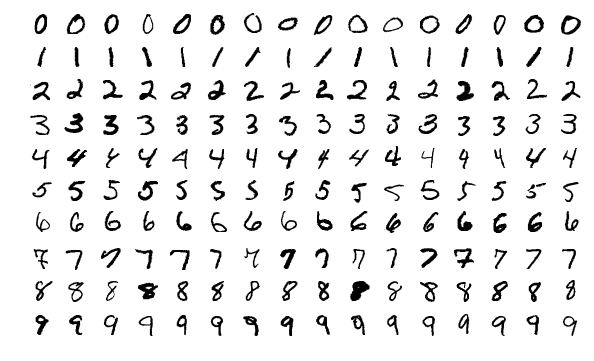
\includegraphics[width=0.8\linewidth]{Figures/Preliminary/mnist}
	\caption[Sample of MNIST Dataset.]{Sample of MNIST Dataset \cite{lecun-mnisthandwrittendigit-2010}. It has been designed for handwritten digit recognition.}
	\label{fig:mnist}
\end{figure}


{
	\begin{tabular}[h]{p{0.05\textwidth}!{\color{gray}\vrule width 2pt}p{0.93\textwidth}}
		&Similar to a child who would be taught to recognize leaves. The teacher shows the child a leaf and describes him what it is. The child will not have enough examples to identify a leaf. \emph{This is a quantity problem.}\\
		&\\
		
		&If a teacher instructs a student to identify a considerable number of things and rewards the student for each accurate answer. In all that was shown, there are many things but very few leaves. Even if they are present, they are largely in the minority. The teacher subsequently invites the student to describe each thing he identifies in front of him and will tend to neglect the leaves. \emph{This is a problem of representativeness.}\\
		&\\
		
		&Ultimately, if the teacher shows the student green leaves. In everything he has learned, he has only seen green leaves and nothing else of that color. Then the student will say every green thing is a leaf. In another case, if the teacher shows a brown leaf, then the student will say it is not a leaf. \emph{This is a bias problem.}\\
		&\\
		&In the end, this teacher/student example is an excellent analogy of Deep Learning that relies entirely on data. To such a degree, the teacher represents the loss, the student, the network. The data is the amount of information that the teacher has shown to the student. And the training is analogous to the framework defined by the teacher.\\
	\end{tabular}
}\\



These three situations show how crucial data is. A significant number of responsibly designed RGB databases have been made available, including ImageNet \cite{imagenet_cvpr09} containing 14 million images, CityScapes \cite{Cordts2016Cityscapes} 25,000 images, MNIST \cite{lecun-mnisthandwrittendigit-2010} 60,000 images (shown in Figure \ref{fig:mnist}), etc.
As a result, the scientific community has been effective to address recurring computer vision issues through common information and benchmarks. These represent reliable utilities since there is a massive amount of data available.

One point that remains important to address is augmentation. Indeed, some tasks do not maintain enough data to be learned, or it is necessary to counter bias in the data. In these cases, the traditional practice remains the augmentation which allows to avoid overfitting \cite{DBLP:journals/corr/abs-1712-04621} or to obtain a consistent data. This established practice allows applying transformations to ensure the invariance of the models to certain phenomena such as rotation, flipping, etc. It consists in the application of operations resulting in photorealistic images. In such ways, the network will be efficient to learn from created data that have not been acquired by a sensor. 



To conclude on the data, we allow ourselves some open questions justifying a majority of the work conducted during this thesis.
Are the widely used datasets representative of all the problems to which they are attached? Are they representative enough to answer faithfully to the problems through colorimetry?
And, is there a learning bias triggered by the use of colorization specifically when the modality is not sensitive to certain physical phenomena?

\subsubsection{Network}
Briefly, the network can be considered as the brain of the algorithm. It is a dynamic structure, composed of layers, which infers from the data a result from the product of its weights.
A network is said to be deep if it includes a hidden layer, i.e. at least three layers.
The trained weight dictionary is commonly defined as a model.

We will focus this section on Deep Convolutional Neural Netowork (DCNN) since it is the most widespread in the field of Computer Vision.

The DCNN concept is based on convolutional layers that act in the same way as standard convolution with a filtering operation. In short, from the convolution of a filter with an image derives an activation map named feature map. 
Convolutional layers sustain two key advantages compared to dense layers. One, convolutions use very few parameters in comparison since this structure forces the sharing of weights over the entire input. Two, they allow, by nature, to be position invariant, unlike the linear operations of dense layers which require priors on the neighboring pixels.
In short, without knowledge of the data and interconnections between pixels, the convolution allows with fewer parameters to extract dense feature maps by operating filters whose weights are fixed through learning. As follows, we exploit the property of this operation to rely on the neighboring pixels to extract the activation map. Ultimately, a network is a succession of layers allowing the extraction of information without having to empirically fix the kernel weights.
Not to forget an important property of convolutions, the dimensionality of the input information is reduced proportionally to the size of the kernels. 


The networks are not only composed of convolution layers, but also of activations, sampling, pooling, etc. which will be addressed explicitly in Section \ref{specnot} for the units used in the presented work.

In conclusion, the principle of the network is to transpose a source image into a desired space through the extraction of features regressed by the loss.



\subsubsection{Loss}

The loss is a minimizable cost function whose target is to attain an optimal objective. From a source image, one operates a forward-pass through the network resulting in a feature map. This map is evaluated through the loss function which means that the network is evaluated through this objective function. Thus, this measure influences the weights of the network through the back propagation.

Briefly on the back propagation \cite{bryson1961gradient}, it allows to fine tune the weights of the network layers to minimize the global error. Thus, starting from the loss and using partial derivatives, the gradient goes up along the network to allow an adjustment of the layers.

To come back to the loss, it is important to note this aspect of Deep Learning has been re-evaluated in the last few years. While before, the consensus of the scientific community was to deepen DCNN, now there is a significant attraction towards coherent loss scaling. Thus, the Deep Learning competition has more or less shifted from a hardware challenge to a theoretical challenge. Nevertheless, there are some cost functions that have imposed themselves to answer some challenges. For example, the segmentation community tends to use the same regularization terms like Cross Entropy Loss or Intersection over Union \cite{everingham2015pascal}. In another domain, depth reconstruction rather addresses loss allowing self-supervision and building self-sufficient photometric comparison terms\cite{godard2017unsupervised}.

Indeed, there are two main types of losses. On the one hand, those that require ground truth and operate a comparison thanks to annotated datasets (the leading case of segmentation). On the other hand, the algorithms that cannot have ground truth and that size the terms to avoid requiring external information (depth map inference). These two aspects explain the movement from supervision to self-supervision and the use of their respective losses. Indeed, tasks requiring supervision like classification and segmentation have been widely investigated and are almost taken for granted. On the other hand, unsupervised processes have become more and more recurrent due to the increasing complexity of the problems addressed.



\subsection{Specific notions}\label{specnot}

\subsubsection{Pooling}
There are multiple types of pooling and two categories. The two categories are: indexed or non-indexed, while the types correspond rather to the applied operations.
The pooling corresponds above all to a sampling whether it is up or down on a $kxk$ windows size. The different operations commonly used are:
\begin{itemize}
	\item \textbf{Max Pooling. } Retains the max value by eliminating the details.
	\item \textbf{Average Pooling. } Considers all important information and averages it.
	
	\item \textbf{Min Pooling. } Implies that "only the details count" and eliminates strong features.
	
	\item \textbf{Probabilistic Pooling. }Draws probabilities for each regions through activation normalization. Then, preserve the highest probability corresponding value.
\end{itemize}

Consequently, depending on the operations chosen, the impact on the feature maps is very different and involves various concepts. As illustrated in Figure \ref{fig:pooling}, the result of these different approaches gives very distinct maps.

\begin{figure}[h]
	\centering
	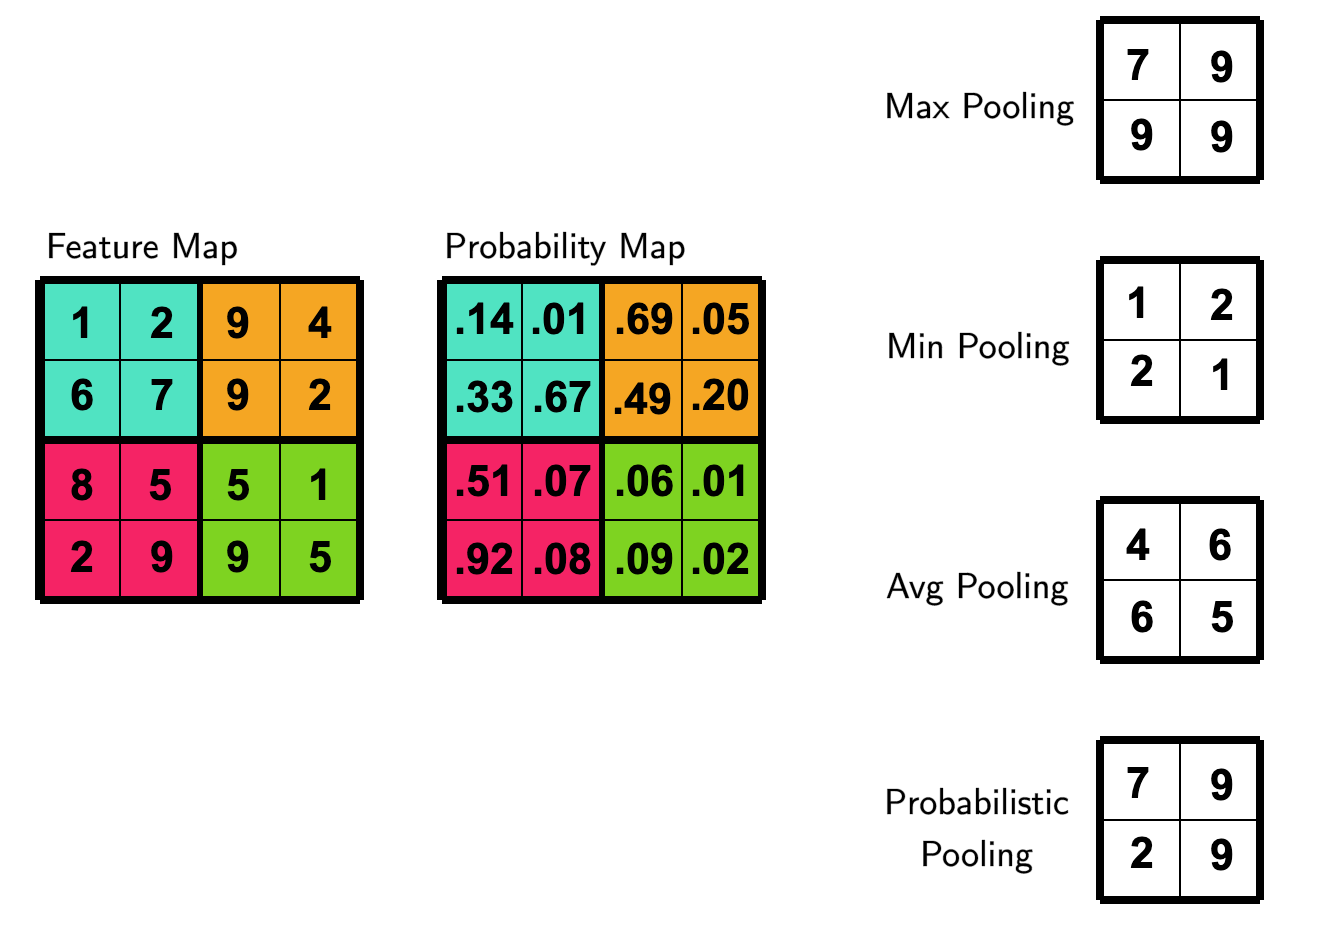
\includegraphics[width=0.8\linewidth]{Figures/Preliminary/pooling}
	\caption{Illustration of different pooling strategies.}
	\label{fig:pooling}
\end{figure}



Then comes the concept of indexing. Indeed, hourglass algorithms do not only downsample but also generally require a return to the original dimensionality. Thus, there are two approaches that imply two different behaviors:
\begin{itemize}
	\item \textbf{Non-indexed. } Place the value in the upper left corner and fill the kernel with zeros.
	\item \textbf{Indexed. } Retrieves the index of the down-pooling layer to place the value at this same position. Fill the rest of the kernel with zeros.
\end{itemize}

Thus these two approaches observe respectively two different behaviors. While one considers that the spatial cue is not necessary for the integrity of the information, the other keeps the positioning and ensures its transmission. As shown in Figure \ref{fig:indexed}, resulting maps differ due to the different techniques.

\begin{figure}[h]
	\centering
	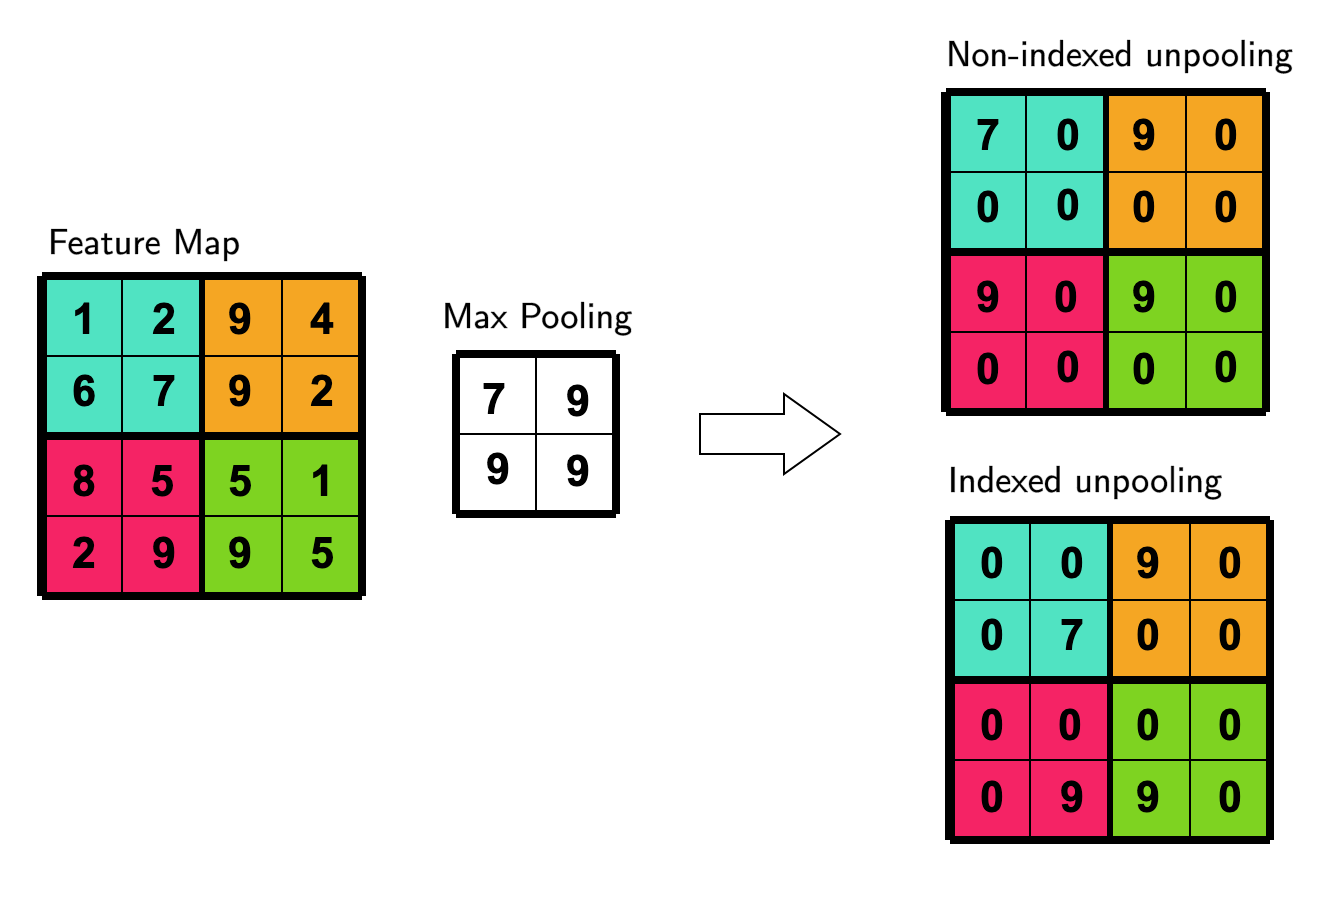
\includegraphics[width=0.8\linewidth]{Figures/Preliminary/indexed}
	\caption{Illustration of indexed pooling.}
	\label{fig:indexed}
\end{figure}


Concluding, pooling is an essential operation that avoids the naive techniques of bilinear sampling. Although this allows to reduce the dimension of the images, through the different methods stated, it is possible to promote behaviors and therefore to infuse these layers with prior knowledge.

\subsubsection{Atrous Spatial Pyramid Pooling (ASPP)}

ASPP\footnote{This architecture is used in Section \ref{abc}.} is a concept created by Chen et al. \cite{chen2017deeplab} to define pooling strategy differently. The principle consists of several dilated convolutions, centered on the same pixel. Thus, one can define a pixel using a succession of convolutions to accumulate different receptive fields. Finally, it is not only a question of reducing the dimension of the image, but also of adding context to the remaining information. 
As a result of each convolution, a number of contextualized features are concatenated and processed by a dense 1x1 convolution. The resulting information will have been impacted by a panel of more or less neighboring information increasing the total impact on the image (receptive field added).
A diagram in Figure \ref{fig:aspp} shows the organization of such a pooling architecture.

\begin{figure}[h]
	\centering
	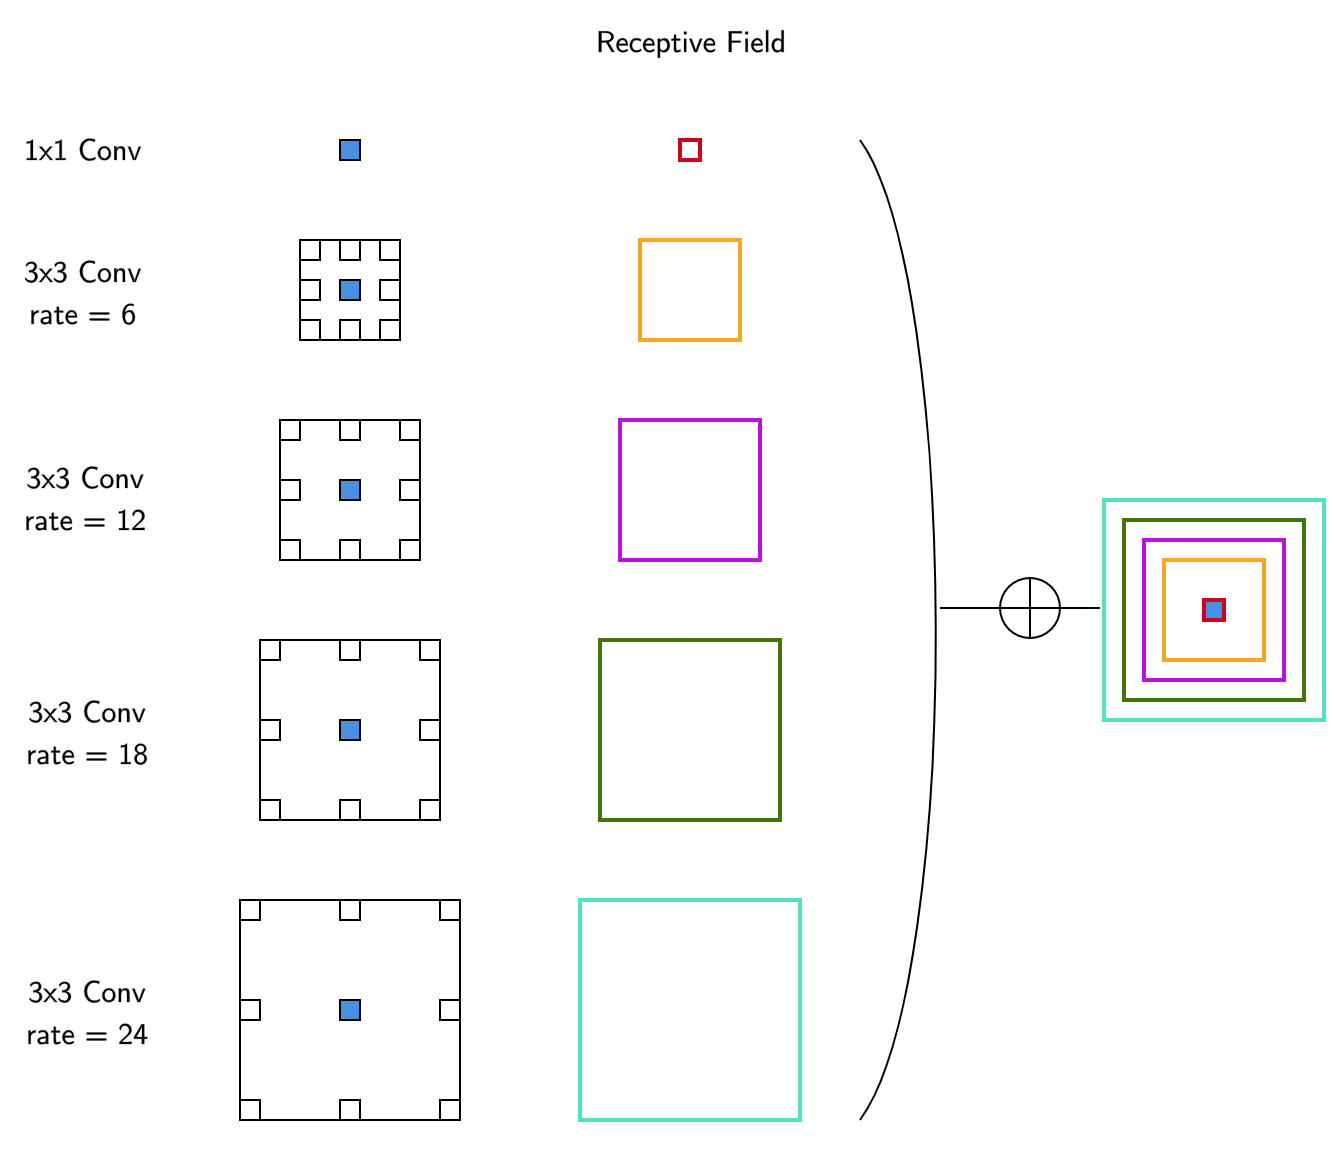
\includegraphics[width=0.8\linewidth]{Figures/Preliminary/aspp}
	\caption{Diagram of ASPP strategy.}
	\label{fig:aspp}
\end{figure}


This technique has been validated in segmenting algorithms and shows that the use of such a process along with other complementary blocks allows a better understanding of the scene. By this, all indications are that this strategy favors the expansion of regions and the taking into account of contours to define dense classes rather than classifying pixel by pixel without taking into account the neighbors.


\subsubsection{Atrous Convolution}

The concept of atrous convolutions has already been briefly expressed above. Indeed, this convolution is identical to a dilated convolution (shown in Figure \ref{fig:aspp}). This operation increases the receptive field, i.e. the impact of the convolution on the original image. This has a particular effect which is to introduce context into the calculation. Instead of considering only the nearest neighbors, one can space the kernel and therefore consider distant pixels.

Thus the convolution atrous has a direct influence on the spatial importance. It is thus a question of finding a compromise between requiring context by strongly dilating the convolutions or forcing the importance of the localization through a tightened kernel.  

\subsection{Conclusion}
This section allowed a visualization of the Deep Learning basics by introducing in turn the data, the network and the loss. 

Through these three essential points, it has been possible to summarize the various key aspects of Deep Learning. In the same way, it was possible to expose the critical aspects of the work presented in this manuscript.
Indeed, since data is a cornerstone of our methods, it is necessary to put open questions that can be addressed throughout this thesis.
Moreover, it has been estimated that the networks and their dimensioning depend largely on the task addressed. 
Finally, the cost function represent the critical element to sustain a safe and valid optimization.
Once these three aspects are reviewed, it is possible to unpack some of the concepts that will be needed for the diverse applications proposed in this thesis. Thus, we have overviewed three specific notions recurrently used in our work. 




% Chapter 1

\chapter{Deep Polarization-Based Semantic Segmentation} % Main chapter title

\label{Chapter4} % For referencing the chapter elsewhere, use \ref{Chapter1} 

%----------------------------------------------------------------------------------------

% Define some commands to keep the formatting separated from the content 


%----------------------------------------------------------------------------------------

This chapter is dedicated to segmented map estimation from a polarimetric image. As described in Chapter \ref{Chapter2}, segmentation represent a rising field in computer vision. In essence, it is a pixel-level classification of images. Moreover, it is possible to add the semantic dimension to the problem to formulate the interconnections of the classes and to add a part of understanding.

In the framework of the presented work, we propose to use polarization as an input modality. While the vast majority of algorithms rely on so-called standard modalities, such as colorimetry, we want to show a change of space can modify, even simplify, the problem of semantic segmentation of complex urban scenes.
As a consequence of this change of modality, we propose reviewing the whole pipeline from the database to the estimation via CNN through the creation of an adequate augmentation procedure.

This chapter is constituted as follows. We briefly introduce our scenario and motivations in Section \ref{intro_4}. In Section \ref{mod_4}, we discuss the modality constraints as well as the choices made to make the polarization usable. Then, in Section \ref{aug_4}, we focus on the augmentation process. 
Finally, Section \ref{net_4} and Section \ref{exp_4} will respectively discuss the networks used and the experiments.
Section \ref{sum_4} summarizes our work.

\section{Introduction}\label{intro_4}

Recently, pixel-wise semantic segmentation (PwSS) has achieved great success especially thanks to the increased computing capacity of modern machines. Yet, a less expensive solution is very little investigated, the moderate use of data and computing power. The formulation of the problem is then marginally different. Instead of loading the networks with a vast amount of data and/or increasing their size, the problem is estimated upstream to discriminate the network.
It is nevertheless notable some contributions are tackling the problem, such as few-shot learning \cite{dong2018few, siam2019amp}. However, a very small minority transpose the data space to apply a constraint ahead of the network rather than impacting the processing core.

We aim to propose a complete PwSS pipeline to describe complex urban scenes based on polarimetric imagery.Here, "complex" defines the possibility of adverse weather conditions and scenes subject to reflection. We start with an observation: urban scenes are prone to specular relfection. Indeed, whether it is the metallic paint of cars, road signs, the presence of windows or even the road in rainy conditions, these surfaces reflect the light.Rather than defining these reactions in a space that saturates in these cases, we propose to implement a modality in which these phenomena are defined.
We then propose using polarization instead of colorimetry which would export its constraints relative to these occurrences. We therefore rely on polarization to simplify the segmentation problem in urban environments.
Thus, we need deconstructing all the achievements in the PwSS domains to reconstruct a polarization-adapted pipeline: the dataset, the image representation, the augmentation and the estimation of the results.

In practice, the methods require massive datasets like KITTI \cite{Geiger2012CVPR} or Cityscape \cite{Cordts2016Cityscapes} that deliver both corresponding input image with a reference segmented map.
These mass requirements are onerous to achieve when implementing a non-conventional modality, which motivates a more measured use of the data.
A straightforward approach would be to acquire a large amount of data and then annotate it to enrich the generalization capacity of the network. Since our approach is alternative, we propose to acquire a limited number of images and use the augmentation to enrich the set.
Although augmentation has been popularized for its advantages in terms of problem generalization and overfitting prevention, it is only viable for interpolable images. In short, as soon as an image is directly related to the physics of the scene, this process is not applicable since it will alter the validity of the observation. On the other hand, since the colorimetry is interpolable and does not report any alteration as a result of it, then the augmentation is valid for this type of image.
In line with the initial objective of the augmentation, we define a group of transforms applicable to polarimetric imaging and in particular, we focus on the physical adequacy of these.
Since it is necessary to benchmark the proposed solution, we tackle the possibility of evaluating our method and especially in competition with the conventional approaches. Aiming this objective, we have aggregated our dataset taking into account that each polarimetric image and segmentation pair correspond to an RGB image and segmentation pair. 
 
\section{Modality-related constraints}\label{mod_4}

As stated previously and more precisely in the Section \ref{Polar_explain}, with polarization follows a set of constraints of its own.
In this section the numerous constraining items of the modality will be discussed. First, the fomulation of the problem with respect to the data will be stated. Then, in part \ref{rep_pol}, the representation aspect of the imagery will be addressed. This chapter will be concluded by the methods operated to aggregate and validate this dataset.

\begin{figure}[ht]
	\centering
	
	\begin{subfigure}[b]{.8\linewidth}   
		\centering 
		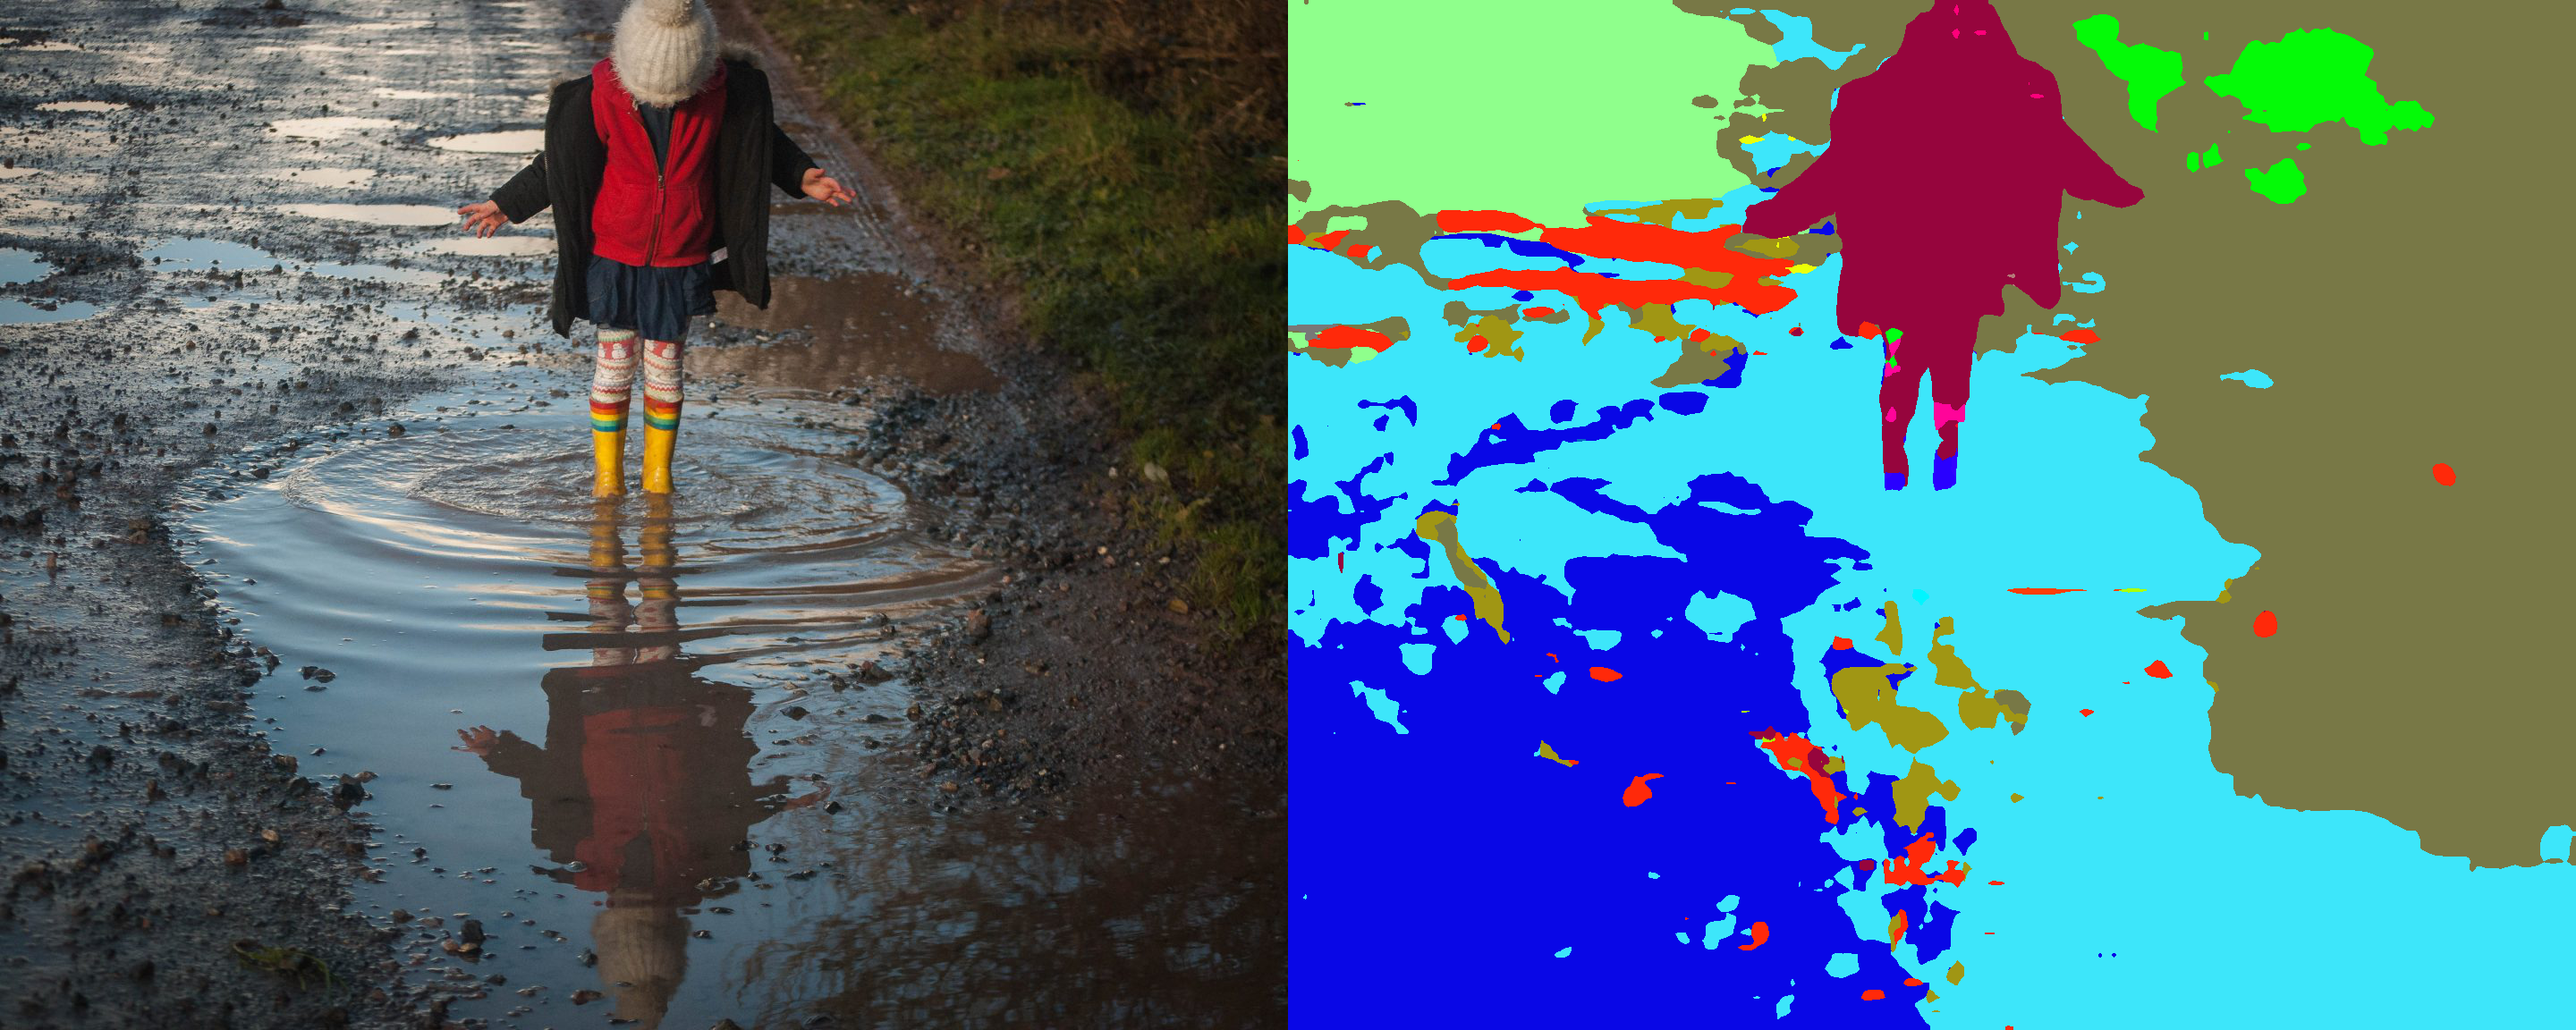
\includegraphics[width=\linewidth]{Figures/Formulation/image_seg_fail.png}
	\end{subfigure}
	
	
	\begin{subfigure}[b]{.8\linewidth}   
		\centering 
		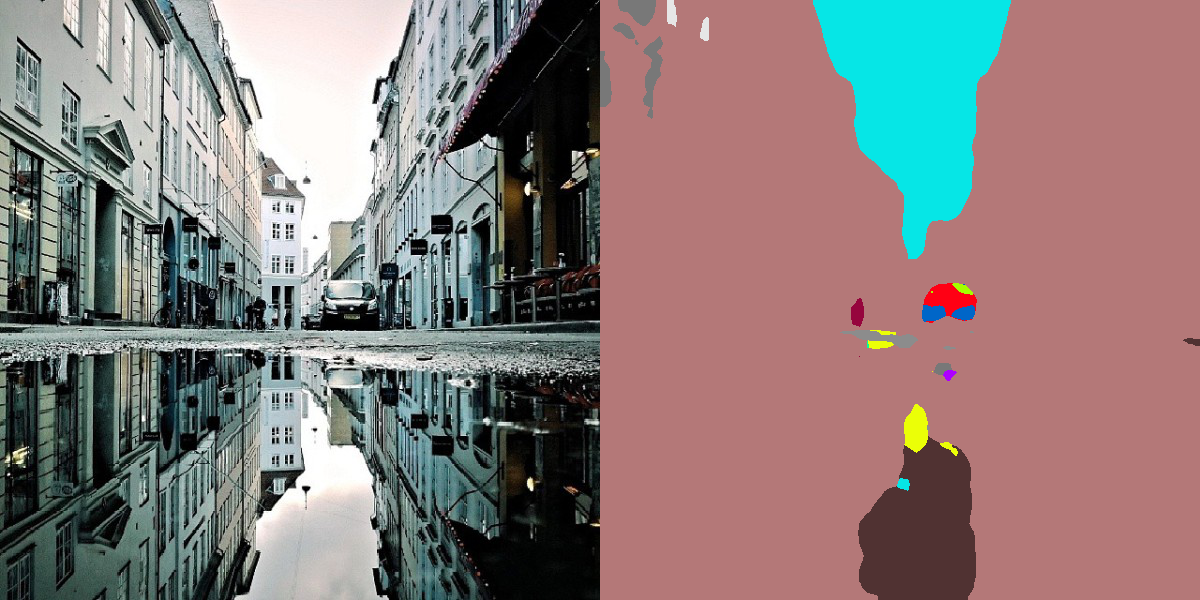
\includegraphics[width=\linewidth]{Figures/Formulation/image_seg_fail2.png}
	\end{subfigure}
	
	
	\begin{subfigure}[b]{.8\linewidth}   
		\centering 
		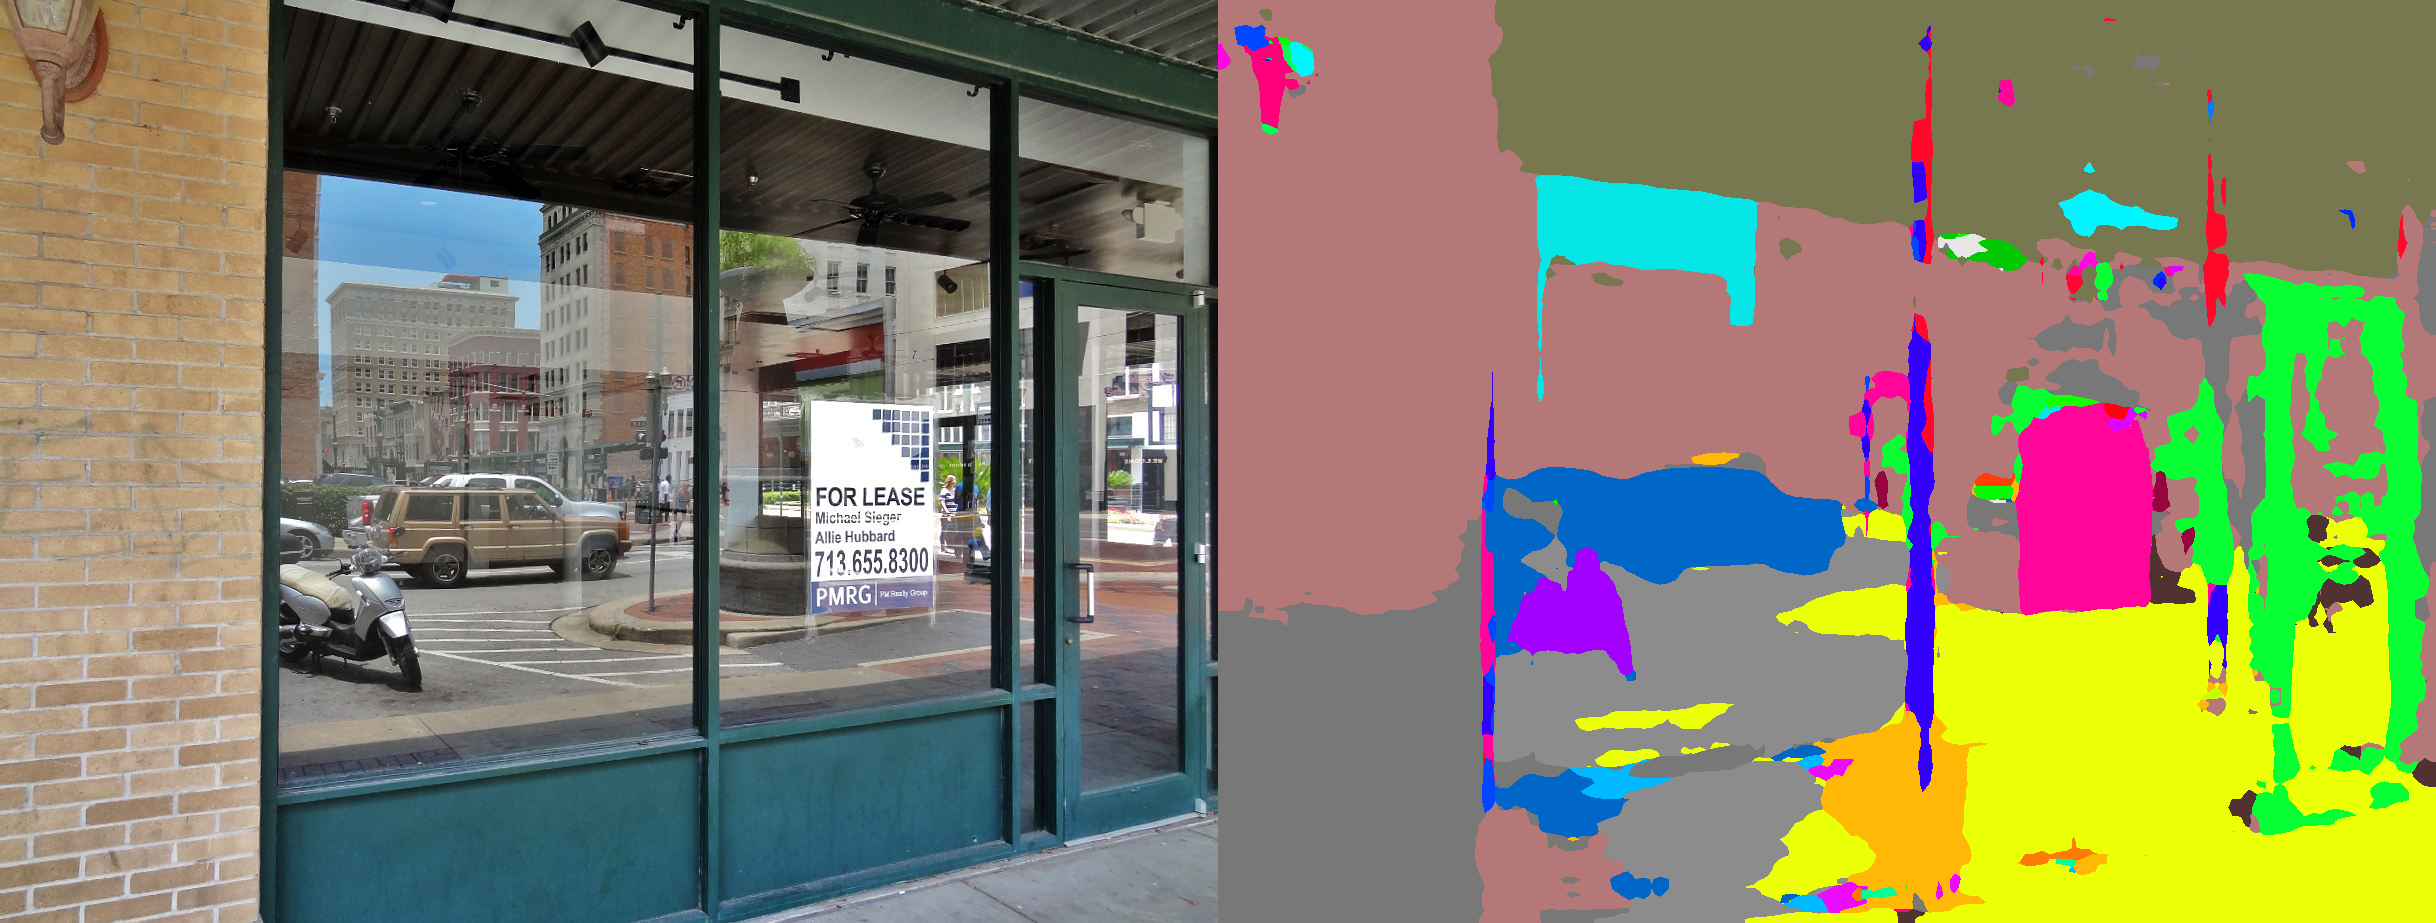
\includegraphics[width=\linewidth]{Figures/Formulation/image_seg_fail3.png}
	\end{subfigure}
	
	
	
	\caption[Reflection erroneous segmentations from RGB]{Segmentation results from \cite{zhou2018semantic} showing erroneous estimation on specular surfaces.}
	\label{fig:fail-seg}
\end{figure}

\subsection{Formulation}\label{form_pol}
With the objective of developing an algorithm relying on reflection to define urban scenes, it is necessary to formulate the problem. As mentioned before, we start from a statement: urban scenes are mostly subject to specular reflection. This phenomenon is even amplified when the weather conditions are unfavorable. Plus, although standard algorithms have acceptable performances in common environments, they tend to fail when they are in the presence of specular reflection, especially when observing puddles. Moreover, the methods are unhelped by the usual datasets since they generally do not contain any of these occurrences.




As shown in the figure \ref{fig:fail-seg}, algorithms that perform well in favorable cases tend to miss their estimate when they observe specularity. This kind of erroneous estimation can be problematic especially if an autonomous vehicle algorithm depends on these estimates.

However, it is necessary to bound the polarimetric images to obtain the desired effect: discriminate and simplify the problem.
Unprocessed, polarization images are not really usable. As described in the Section \ref{Polar_explain}, the images are sparse and not particularly descriptive. If the raw images are preserved, it is challenging to constrain the problem since the specularity is only defined by the pixel saturation. Although it is indeed characterized, it is necessary to transpose these images through the Stokes parameters to implicitly extract the informative part of the images. Consequently, and in order that the images are exploitable by a CNN, it is necessary to decide on an exploitable representation image.


\subsection{Image Representation}\label{rep_pol}

One critical point of machine understanding approaches is to have representative and understandable images. 
Image representation is omnipresent in the field of computer vision. On the other hand, it has become progressively transparent. The colorimetric images are subject to an image representation allowing to pass from the lowest level (raw) the Bayer matrix, to a composition in three channels, traditionally RGB.
Polarization is not exempt from this, however, since the modality is unconventional and not as widely used, it is necessary to define advantageous rules to the future processing pipeline.

Our goal is to have a reliable and representative image while making it deep learning-friendly. Thus, according to our problem the images must intrinsically represent polarization and by extension specularity while preserving differentiable textures allowing the network to learn. 
Starting from the raw images, we recover the informative part of the images by computing the Stokes parameters:

\begin{equation}
S = \begin{pmatrix}s_0\\s_1\\s_2\\s_3\end{pmatrix} = \begin{pmatrix}P_H + P_V\\ P_H - P_V\\ P_{45} - P_{135} \\ P_R - P_L\end{pmatrix} = \begin{pmatrix}P_0 + P_{90}\\ P_0 - P_{90}\\ P_{45} - P_{135} \\ 0\end{pmatrix},
\end{equation}

where $s_n$ is the $n^{th}$ Stokes parameter and $P_\Theta$ is the dense polatization image corresponding to the $\Theta$ angle oriented polarizer.
It is notable that the $P_\theta$ images must be dense and therefore that between the raw imagery and these, it may be necessary to interpolate the images between pixels to densify them. This will depend mainly on the image resolution of the camera.
Also, recall that in the absence of a quarter-wave plate, no circular polarization $s_3$ is acquired.
From these, it is possible to easily find the three strong descriptors of the polarization, the intensity $\iota$, the polarization angle $\alpha$ and the degree of polarization $\rho$:
\begin{equation}
\iota = \frac{P_0 + P_{45} + P_{90} + P_{135}}{2},
\end{equation}
\begin{equation}
\rho = \sqrt{\Bar{s_1}^2 + \Bar{s_2}^2},
\end{equation}
\begin{equation}
\alpha = \frac{1}{2}\textrm{tan}^{-1}(\frac{s_1}{s_2}),
\end{equation}

where $\bar{s_n}$ is the $n^{th}$ Stokes parameter normalized by $s_0$.

Although there are a multitude of possibilities to combine these three images, it is necessary to consider their nature to obtain a representative result.
While $\iota$ is the texture of the image, it is a standard grayscale image, $\alpha$ and $\rho$ are two complementary images respectively the angle of projected reflection and its "strength". It is then necessary to aggregate this information to maintain the integrity and especially the interest of the polarization. Thus, the raw concatenation would strongly reduce the interest of the imaging for PwSS applications.

Also, to avoid imposing a relearning of the organization of the pixels for the network, but also to benefit from the advantages of the transfer learning, it is necessary to move towards a three-channels structure.

\begin{figure}[h]
	\centering
	\begin{subfigure}{.4\textwidth}
		\centering
		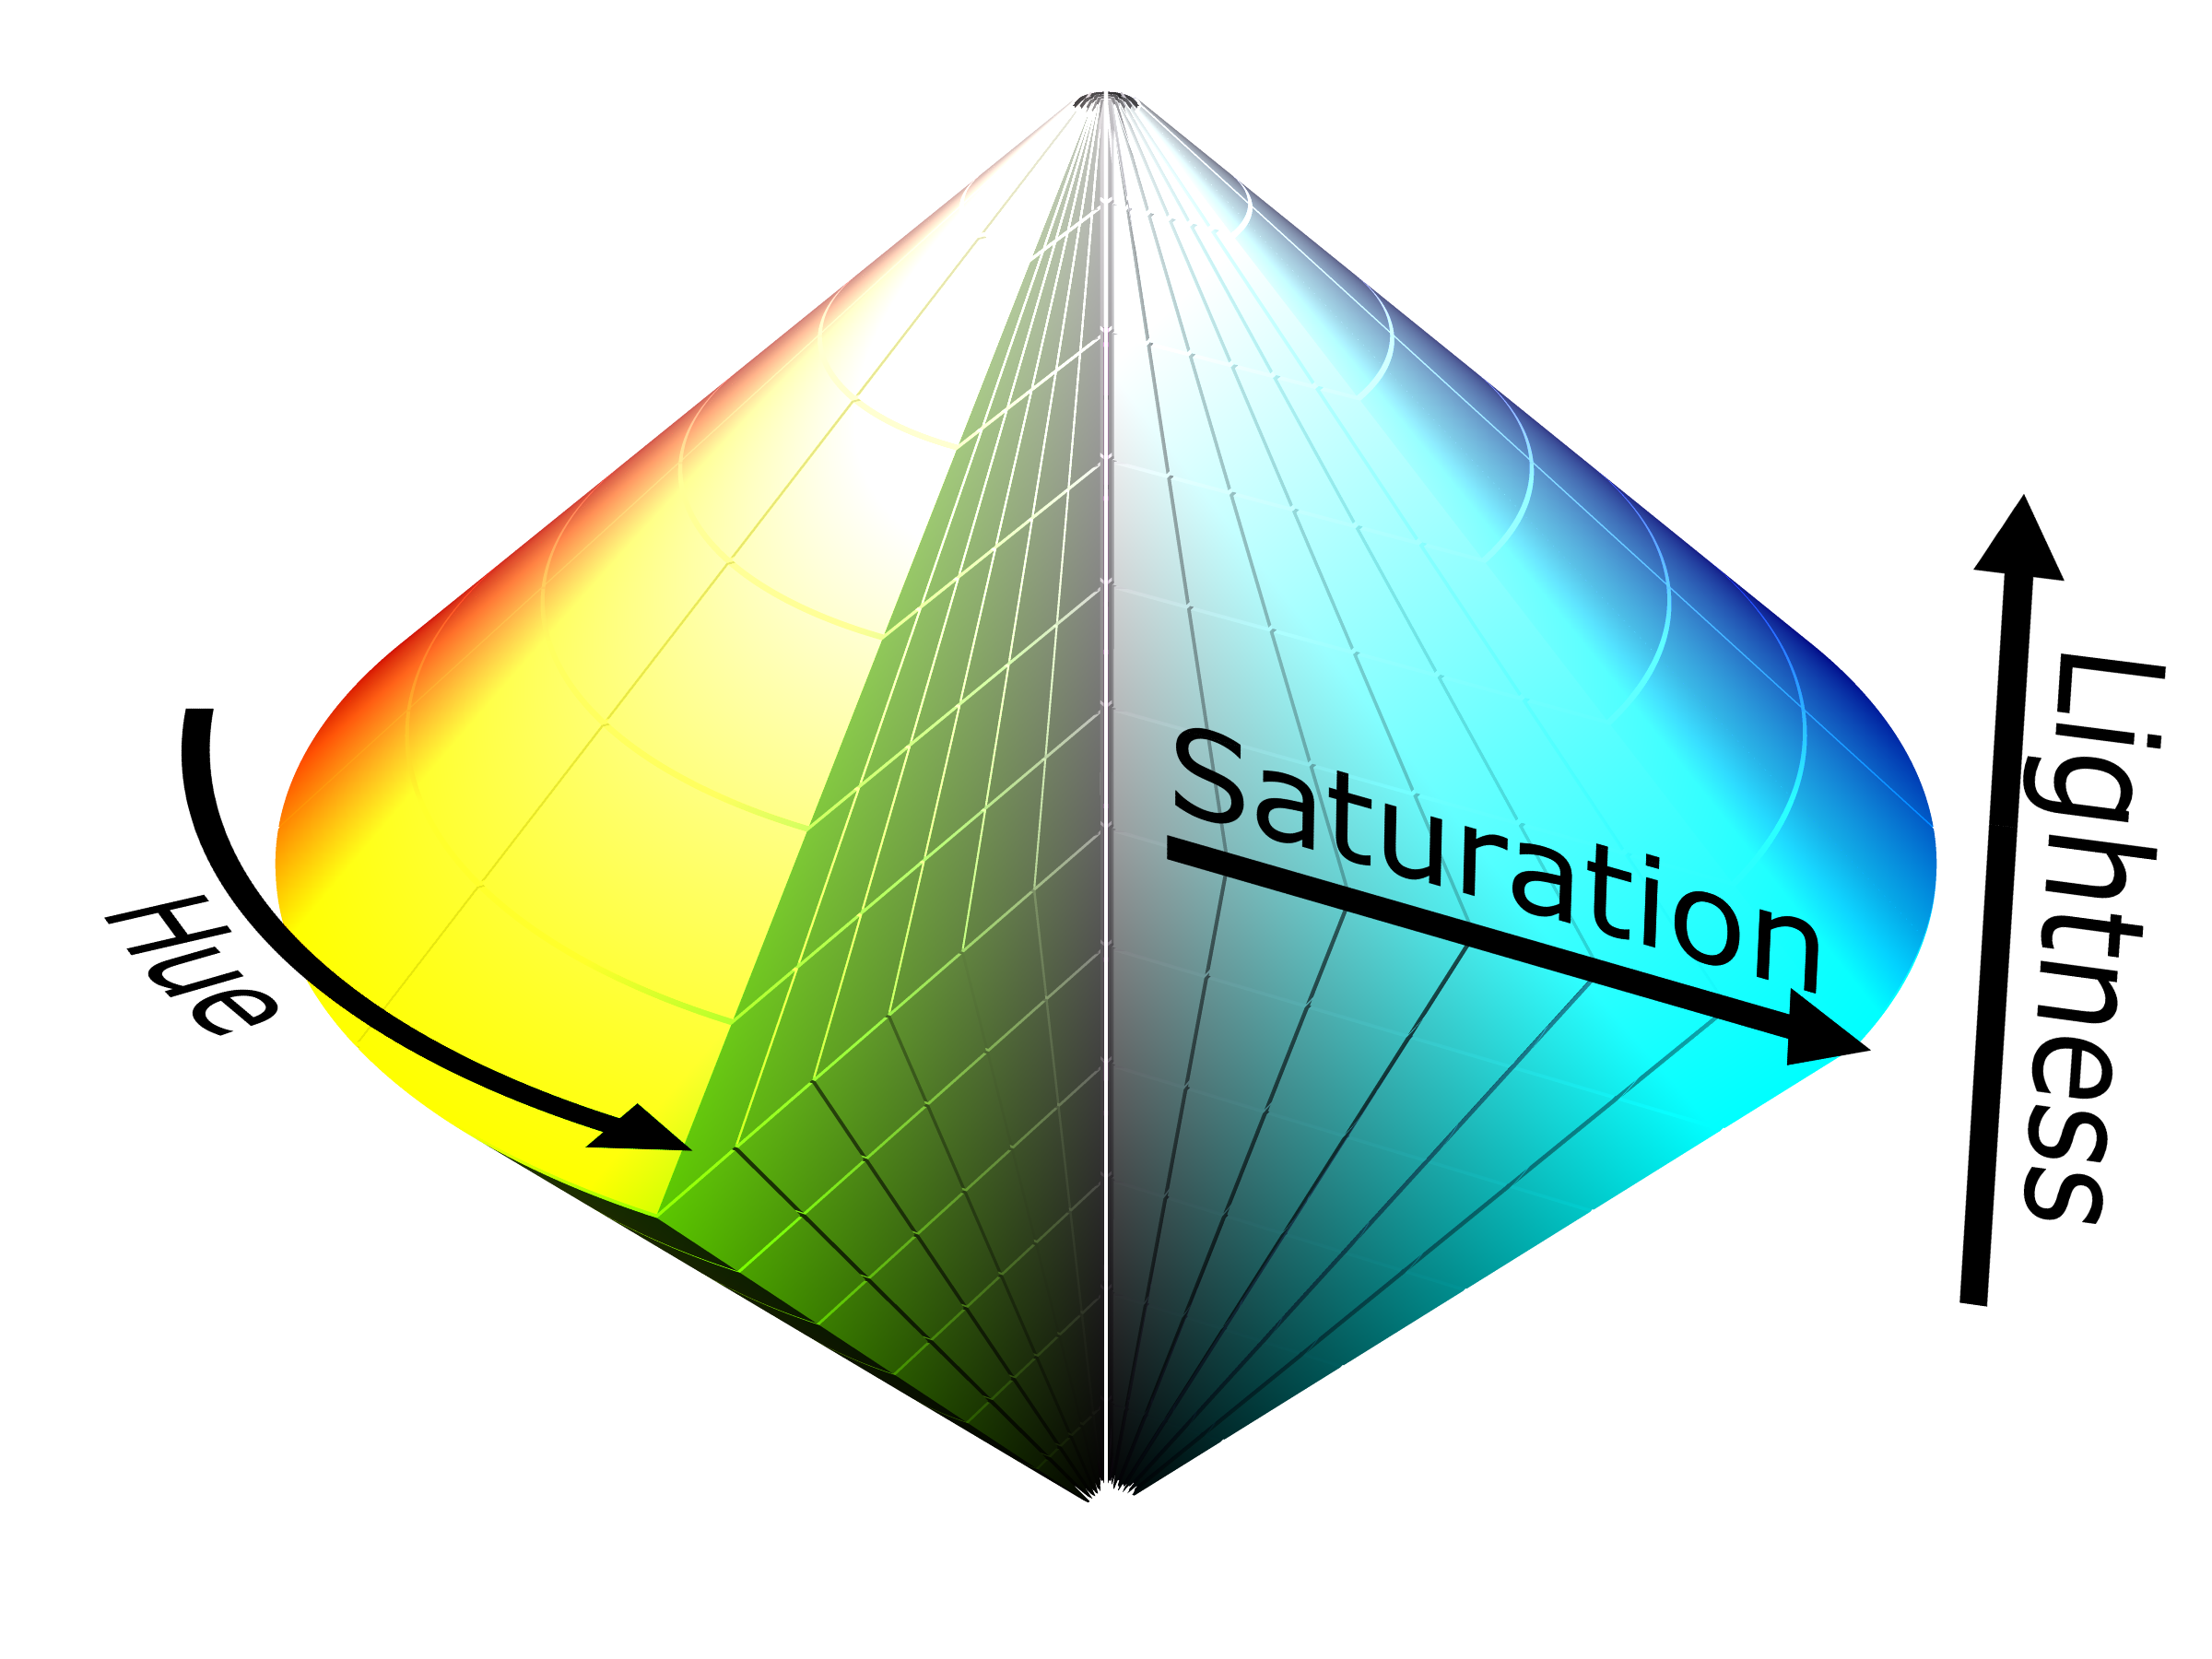
\includegraphics[width=\linewidth]{Figures/Representation/HSL_block.png}
	\end{subfigure}
	\begin{subfigure}{.4\textwidth}
		
		\centering
		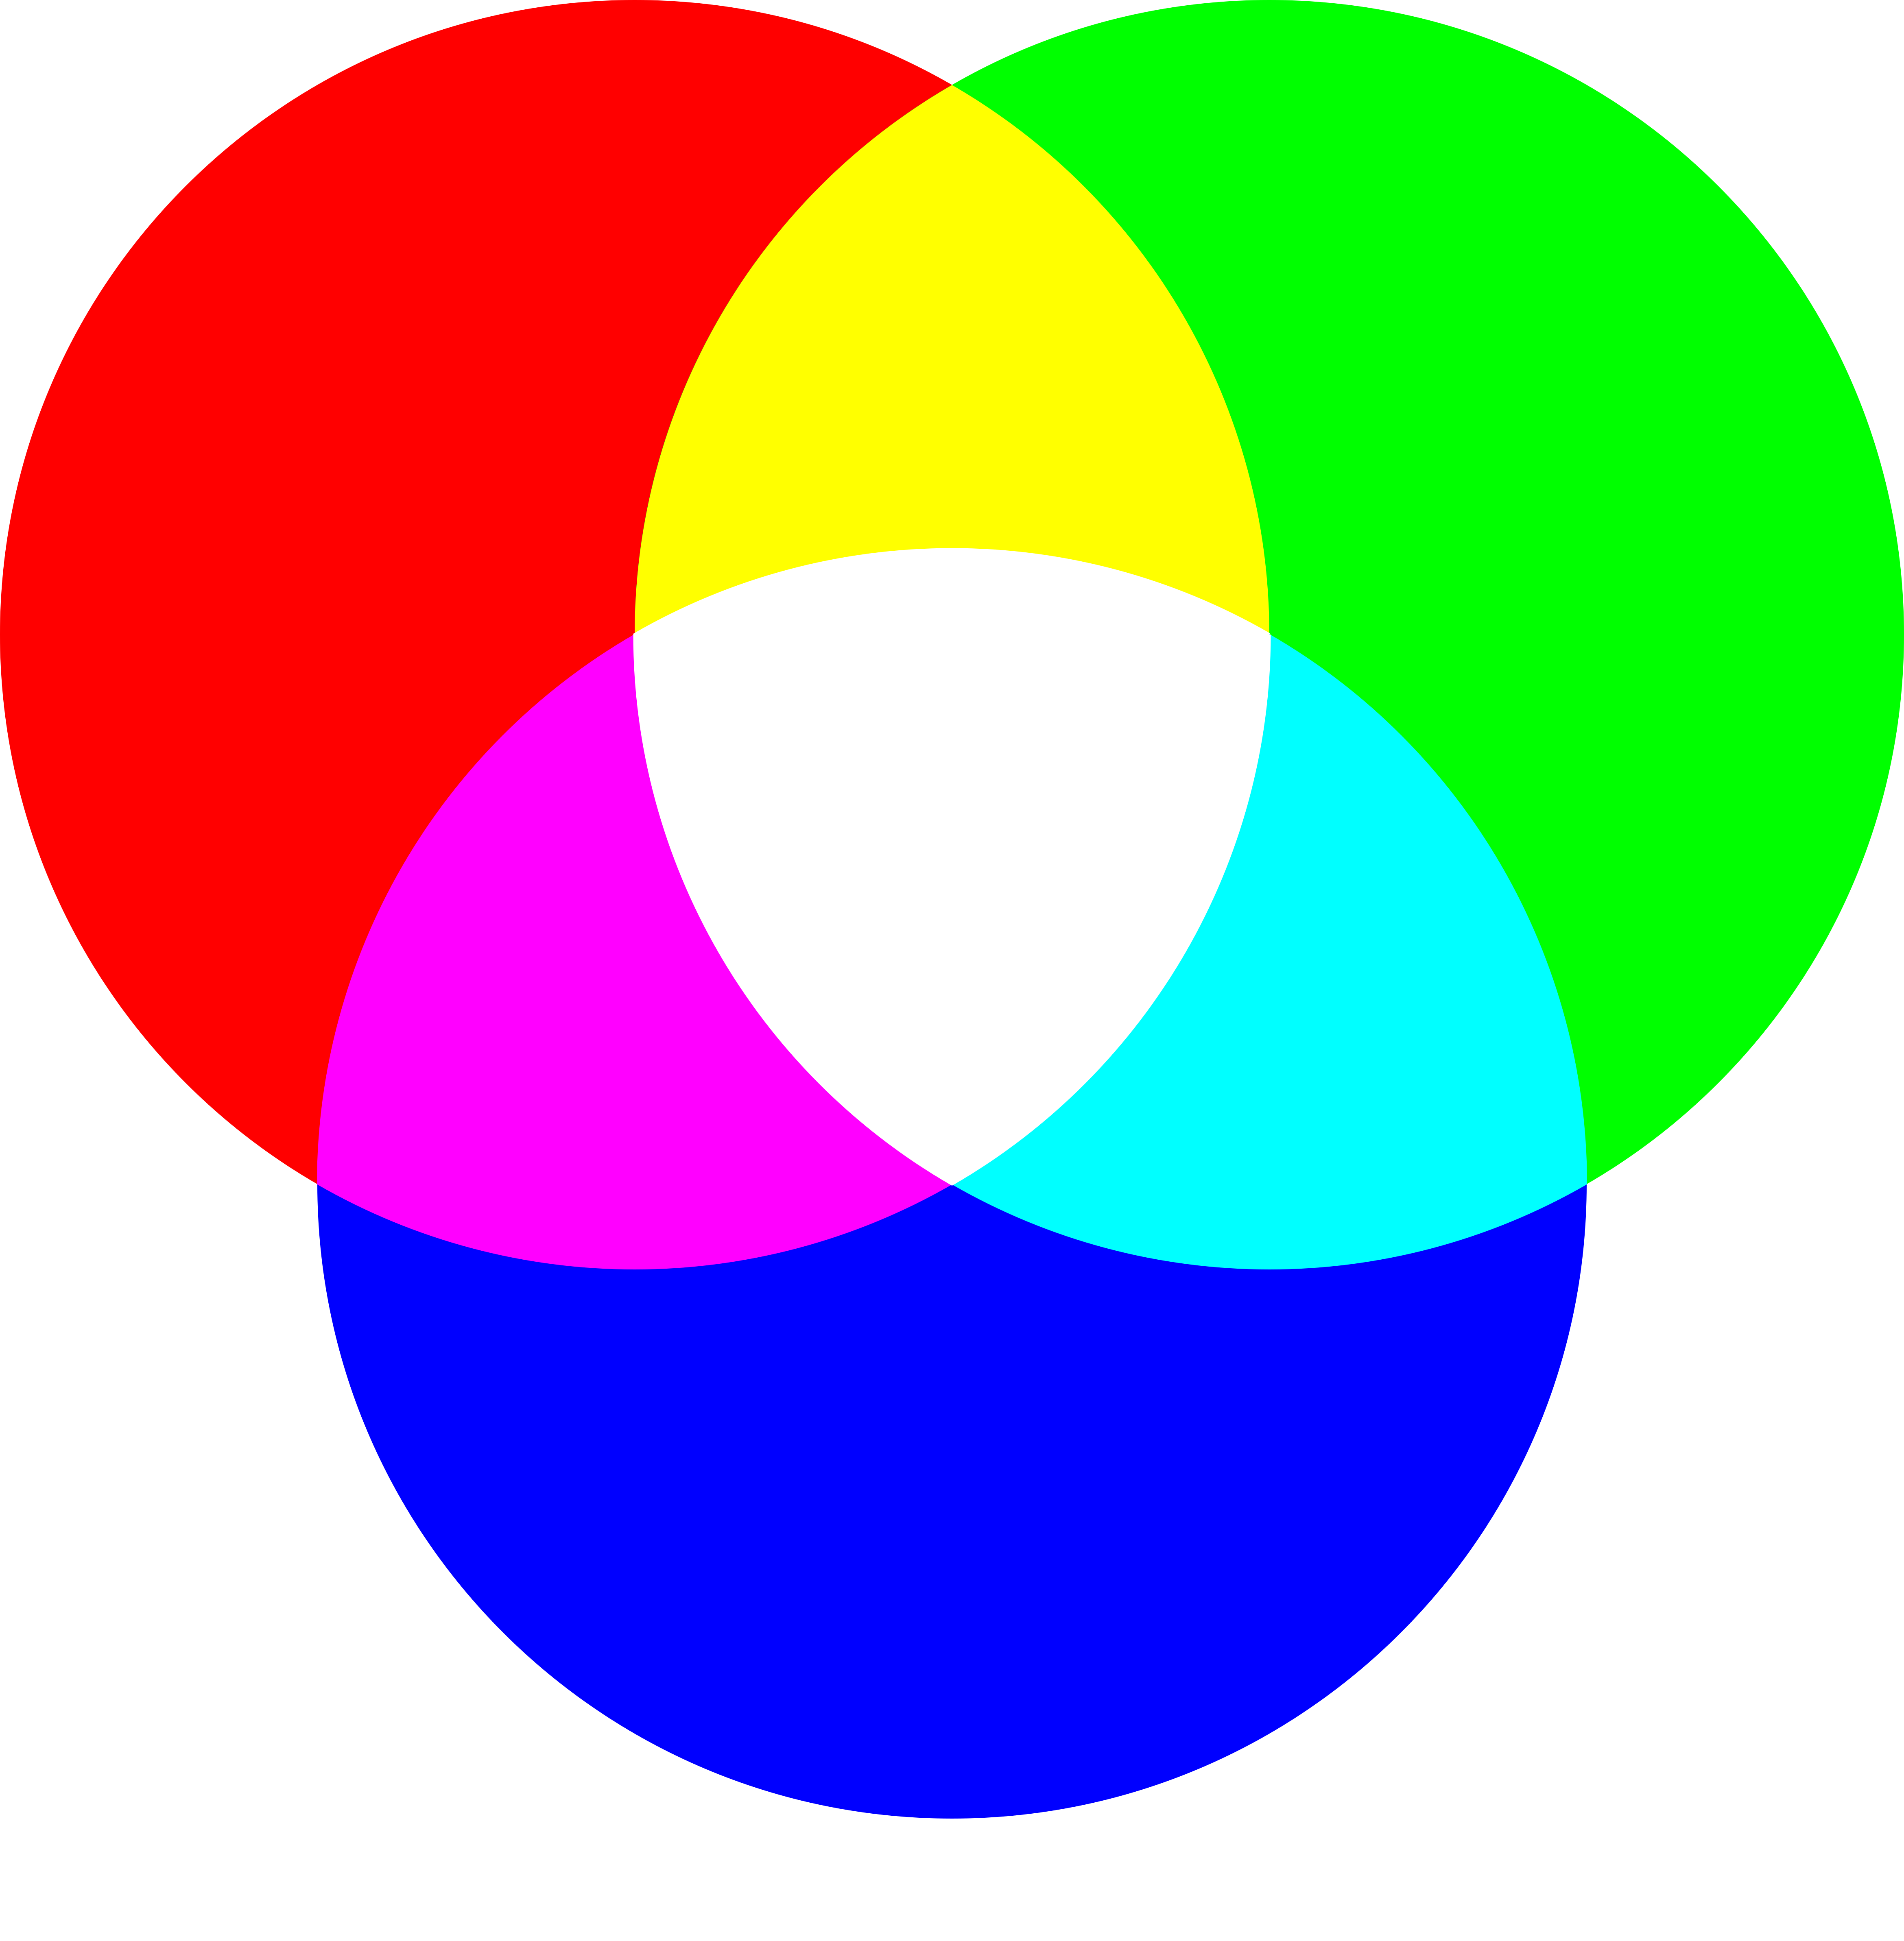
\includegraphics[width=.7\linewidth]{Figures/Representation/RGB_wheel.png}
	\end{subfigure}
	\caption{HSL and RGB color models.}
	\label{fig:hslrgb}
\end{figure}


In this context, we propose representing these images in three HSL channels as proposed by \cite{wolff1995polarization} that will finally be transposed in RGB color space\footnote{Converting toolbix available at: \url{https://github.com/BlanchonMarc/InterPol}}. Indeed, this intermediate format allows infusing particular properties to the image, while keeping a simple transposability from HSL to RGB. As shown in the Figure \ref{fig:hslrgb}, both modelization formats include a singular behaviour.

The RGB model is widely operated since it is direct and additive. In contrast, Hue Saturation and Luminance (HSL) is somewhat different due to its cylindrical and cyclic nature. This model enjoys many advantages, but the prominent attraction for polarimetry is that its channels are neither bounded nor processed in the same way. They are therefore independent but complementary for visual representation.
The key advantage of the HSL representation is its channel coding.Indeed, the three separate channels are quantized differently and allow a direct adaptation with the polarization.
Hue represent a cyclic value between 0 and 360 which comfortably accommodates a $2\pi$-periodic value and thus the polarization angle.
The saturation represents the intensity of the color indicated by the Hue. It is a percentile value that allows an analogy with the degree of polarization. The correspondence between the color and its intensity of this mode is convenient to use with polarization and the proper properties of $\alpha$ and $\rho$.
Finally, L, the luminance, can easily accommodate the intensity value $\iota$ since its utility is very similar to the encoding of a texture.
In conclusion, the polarimetric images will be mapped as:

\begin{equation}\label{eq:hsl}
H \longrightarrow 2*\alpha,  \quad S \longrightarrow \rho, \quad L \longrightarrow \frac{\iota}{255}.
\end{equation}

\begin{figure}[h]
	\centering
	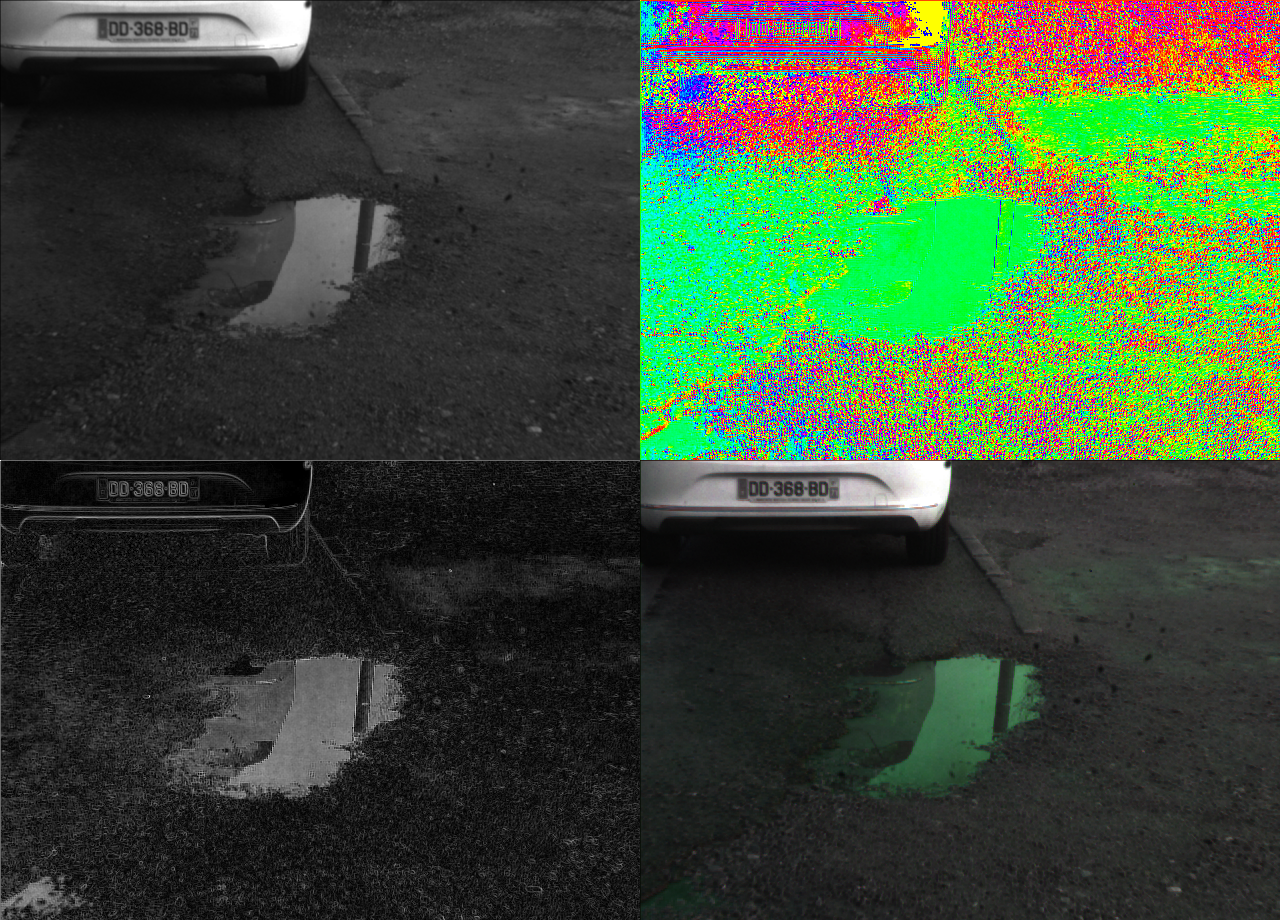
\includegraphics[width=0.8\linewidth]{Figures/Representation/4im}
	\caption[HSL representation of polarization.]{HSL representation of polarization. At the top left is the intensity $\iota$, then at the top left the polarization angle $\alpha$. At the bottom left is the polarization degree $\rho$ and at the right is the combination of the three informative images in HSL format and the equation \ref{eq:hsl}.}
	\label{fig:4im}
\end{figure}


As shown in the Figure \ref{fig:4im}, it is remarkable that the images are peculiar and that their hue is unnatural. Indeed, the texture is present but colors are affected according to the $alpha$ orientation. Also, the intensity of the color is decided by $\rho$. In the end, the more a zone is colored, the more it is polarized. And according to the color, the various angles are observable in a transparent way.

After this representation, a three-channel image is obtained which could be used as input for a DCNN. 
Regrettably, remarkably few models are trained with HSL-mode data, and the convention is until now RGB for the training task. 
Rather than having to end-to-end train a network by training the data encoding, it is more convenient to use RGB. Indeed, this will allow using pre-trained networks and thus to benefit from approved transfer learning methods.
As follows, the choice is considered to transpose the HSL images in RGB while keeping the particular display properties following the system:

\begin{equation}
	C = (1 - |2L - 1|) \times S,
\end{equation}
\begin{equation}
	X = C \times (1 - \Big| \frac{H}{60^\circ} \mod 2 - 1 \Big| ),
\end{equation}
\begin{equation}
	m = L - \frac{C}{2},
\end{equation}
\begin{equation}
	(R^\prime,G^\prime,B^\prime) = 
	\begin{cases}
		(C,X,0) & \mbox{, }0^\circ \leq H < 60^\circ  \\
		(X,C,0) & \mbox{, }60^\circ \leq H < 120^\circ \\
		(0,C,X) & \mbox{, }120^\circ \leq H < 180^\circ \\
		(0,X,C) & \mbox{, }180^\circ \leq H < 240^\circ \\
		(X,0,C) & \mbox{, }240^\circ \leq H < 300^\circ \\
		(C,0,X) & \mbox{, }300^\circ \leq H < 360^\circ  
    \end{cases},
\end{equation}
\begin{equation}
	(R,G,B) = \Big( (R^\prime+m)\times 255, (G^\prime+m)\times 255,(B^\prime+m)\times 255 \Big).
\end{equation}

After all these transformations to interpret the polarization, a polarimetric RGB-coded image is obtained.


\subsection{Dataset}\label{data_pol}

The dataset is a critical element when using machine learning algorithms. The scientific community agrees it is one of the most crucial points if not the most important.
Conventionally, since DL-based methods are greedy, the more data the better. This is accommodating when using a widespread and easily acquired modality. On the other hand, when addressing non-conventional modalities, the major obstacle for the community is the need for a massive amount of data.

Our approach is somewhat alternative although also constrained by modality. The idea is to obtain viable results with the limited data available.
First, it is necessary to acquire data in urban areas and under adverse conditions.

We constituted Polabot\footnote{Available at: \url{http://vibot.cnrs.fr/polabot.html}}, a multimodal oriented dataset composed of 3 synchronized modalities: polarization, colorimetry and near infrared, acquired with the cameras referenced in Table \ref{carac}. 
As a final image collection, it is composed of 178 multimodal aligned, synchronized and annotated urban scene images with eight unique classes: unlabeled, sky, water, windows, road, car, building and none. Unlabeled corresponding to segmentation errors during manual annotation and none being the areas defined as irrelevant for our application. The different scenes propose several complex scenarios composed of puddles or buildings' windows which are often incorrectly estimated in usual methods.
Since this collection is very restricted and insufficient to train a sustainable model, the augmentation presented in Section \ref{aug_4} represent a required requirement.

Yet, the acquisition of this dataset involves two major challenges prior to the augmentation: the synchronization of images from several sources and their alignment which will be respectively presented in \ref{sync} and \ref{align}.

\subsubsection{Synchronization}\label{sync}

One of the problems of acquisition of any multimodal and multifocal system remains the synchronization of images. To be specific, desynchronization can cause a detrimental effect when images are captured at high speed. A shift and the images do not exhibit sufficient correlation due to the distance traveled between two image triggers.
In our case, the de-synchronization is negative for this distance problem but also specifically for the cross-modality performance comparison. Indeed, as previously stated, this dataset allows us to train networks but also and especially to have a point of comparison to determine the advantage of a modality over another for our application.
To prevent desynchronization errors, we have developed a rule-based system\footnote{Available at: \url{https://github.com/BlanchonMarc/Ros_AcquisitionFromTopics}} to ensure the smallest possible cross-modality shift.

\begin{figure}[h]
	\centering
	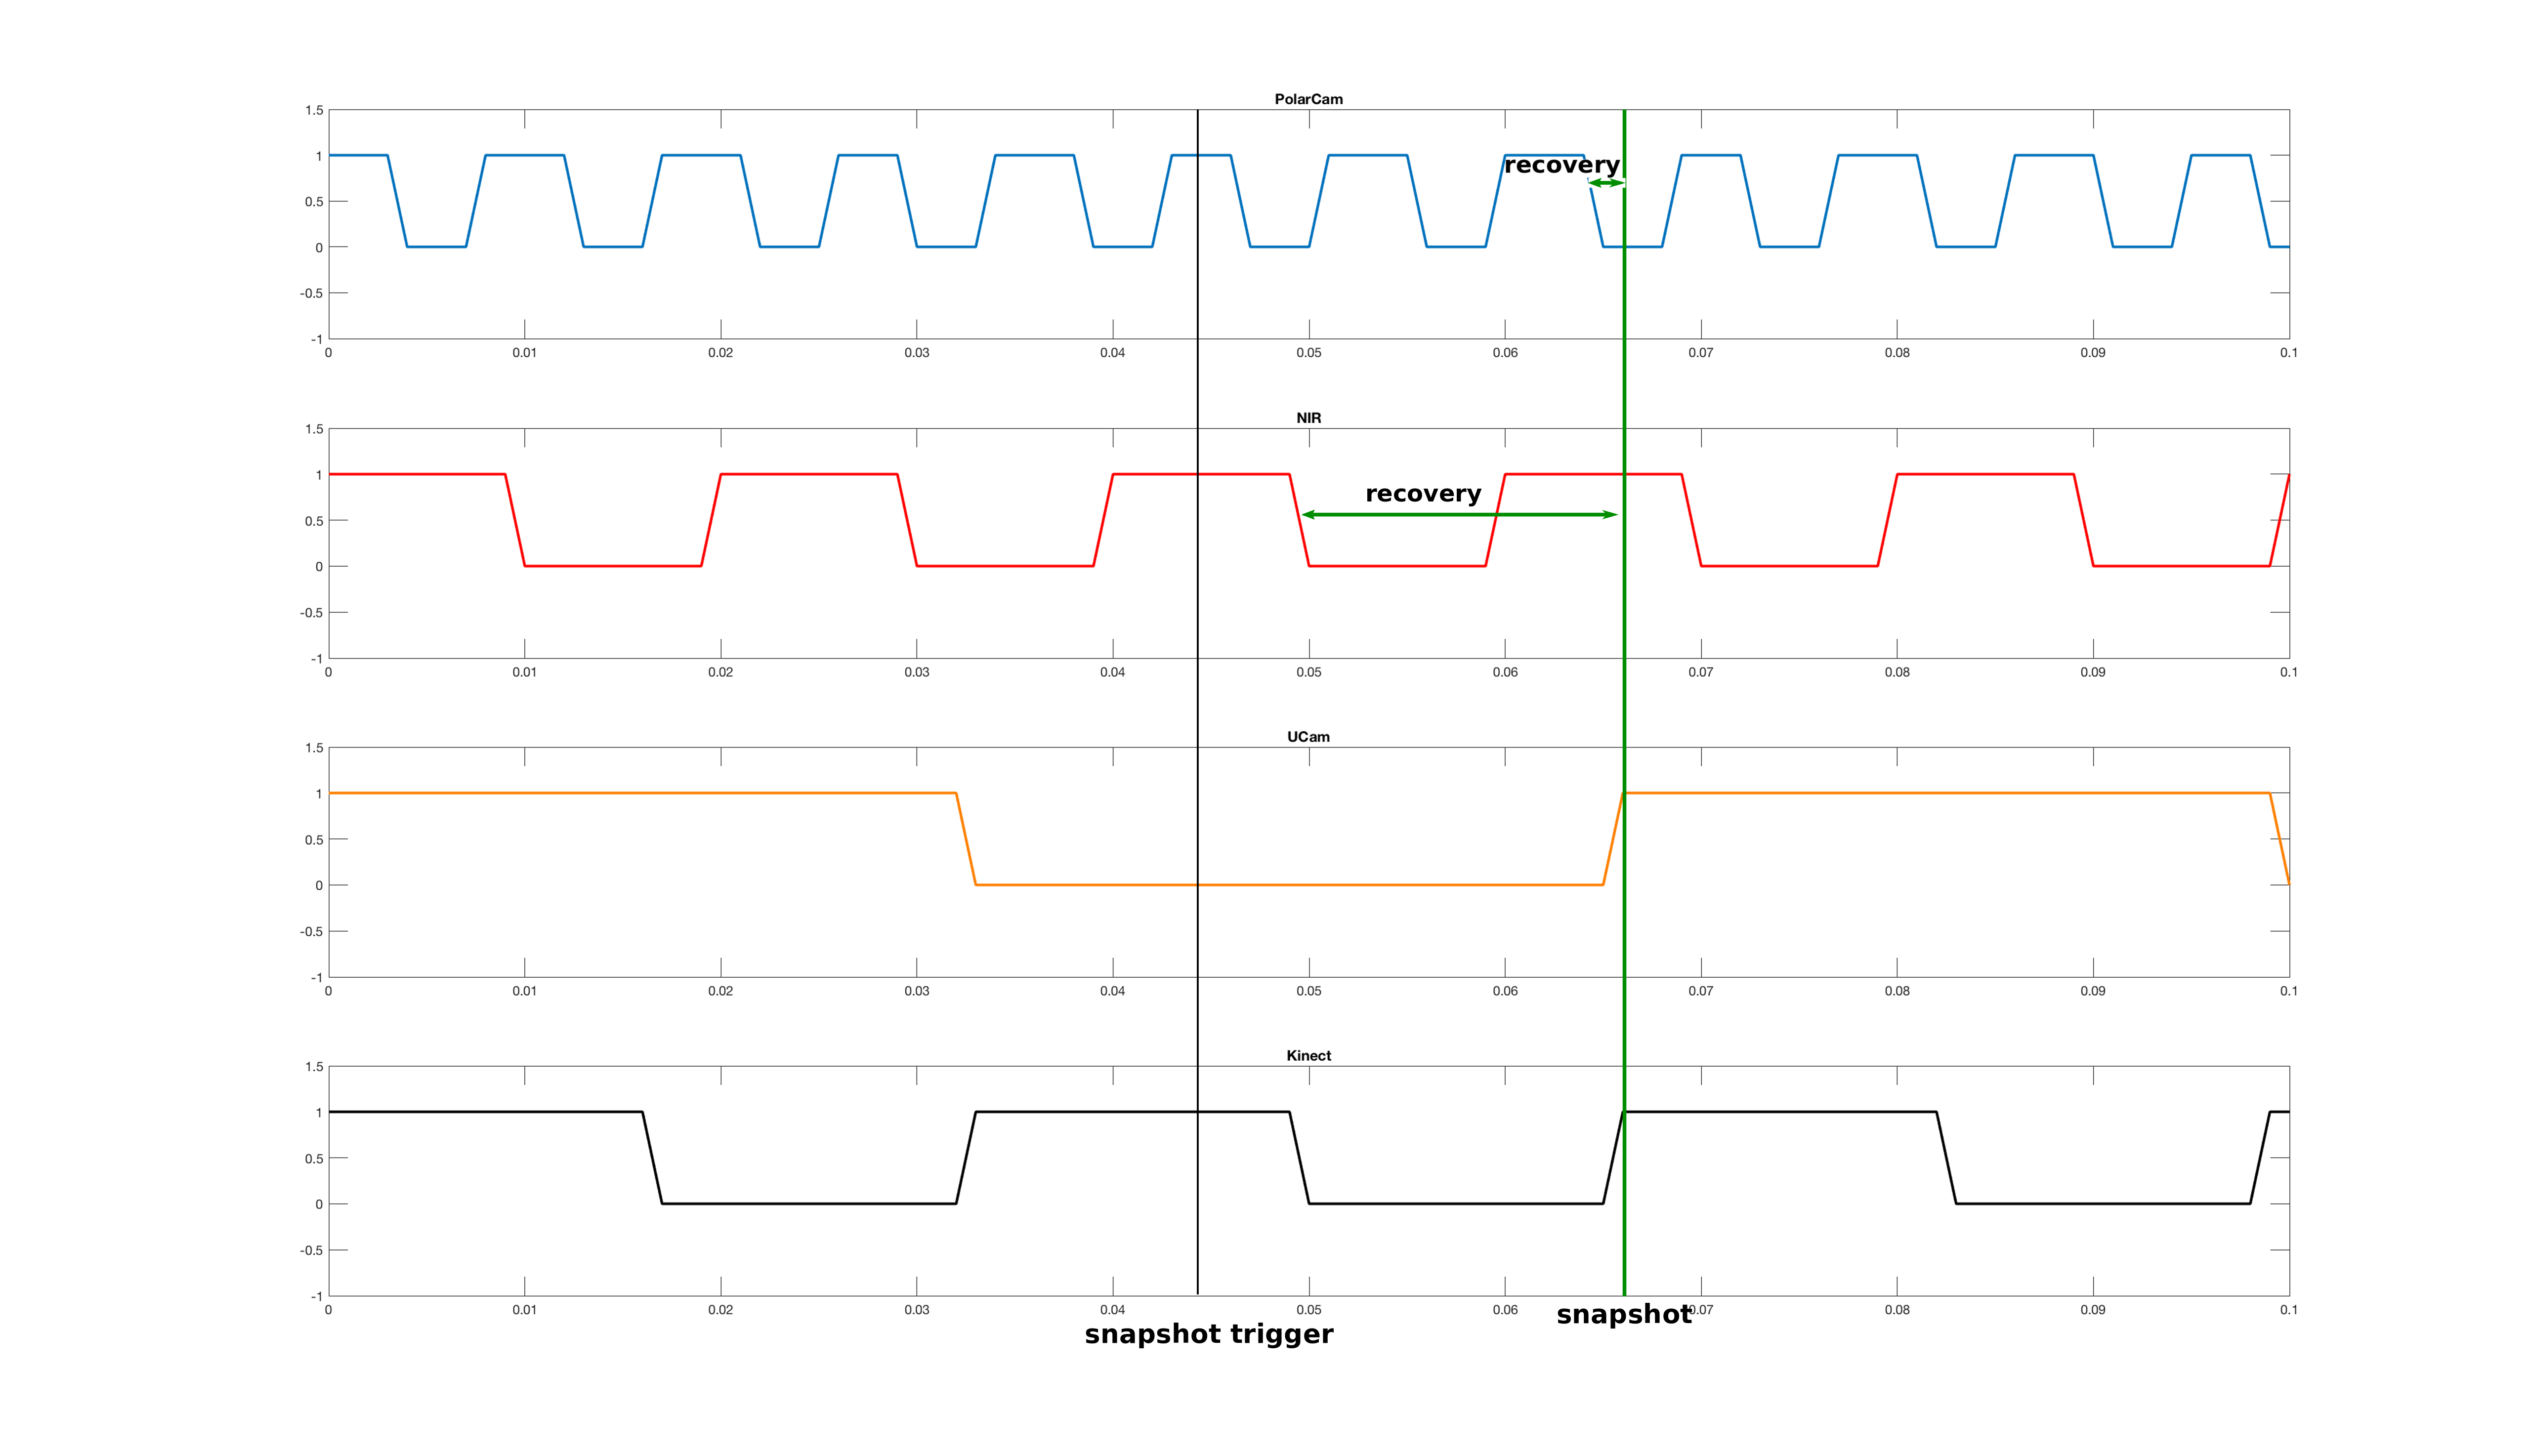
\includegraphics[width=0.8\linewidth]{Figures/Dataset/freqgraphnew}
	\caption{Recovery strategy-based synchronization.}
	\label{fig:freqgraphnew}
\end{figure}


The principle is to consider snapshot trigger signal. The cameras have a discontinuous image stream and this can be represented by square signals. As shown in the Figure \ref{freqgraphnew}, each rising edge corresponds to an image trigger (replacement of the previous image). The strategy is simple, at each artificial trigger, it is necessary to wait for the following acquisition of the slowest camera and then use a recovery strategy.

In conclusion, this simple rule-based strategy allows to drastically reduce the problems related to desynchronization and therefore to eliminate artifacts such as shift, motion blur or displacement between images.

\subsubsection{Multimodal Alignment}\label{align}

Image alignment represent a well-known field. Very well defined, this problem is for the most part solved. However, when addressing the idea of multimodal alignment, known methods can be inefficient, especially when the images to be aligned are non-interpolatable.
This is indeed the case handled in this section. The concept is to efficiently align an RGB image with a polarimetric image. It is significant to experience a precise framing since the correspondence at pixel level must be exact. Thus, a valid comparison can be performed between the segmentation results from independent networks addressed on different modalities.

\textbf{Homography-based.} Homography \cite{artin1957geometric,baer2005linear} is one of the most popular methods to estimate the displacement between two images. Assuming that two images are on the same plane in space then they are linked by the homography. 
There is on top an underlying assumption that the two images must be in the same feature space. This is not the case between colorimetric and polarimetric imaging. However, it is completely possible to find a common space in grayscale intensity.
\begin{figure}[h]
	\centering
	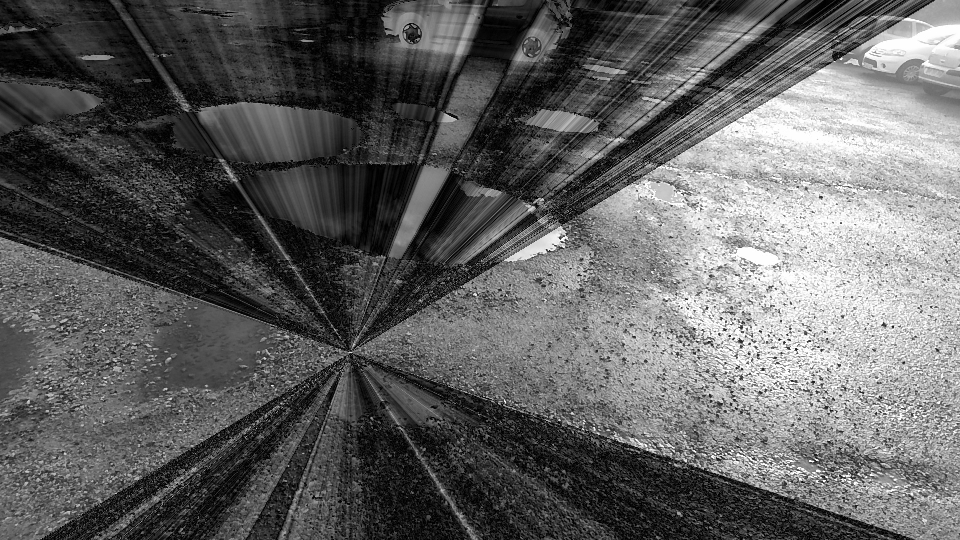
\includegraphics[width=0.8\linewidth]{Figures/Dataset/VISWarp}
	\caption{Innacurate alignment through homography estimation.}
	\label{fig:viswarp}
\end{figure}
Then, just find and map the corresponding feature points on each image and deduce the transformation. The result is $R$ and $t$, the rotation matrix and the translation vector that allow to transform an image to align it with another one. 
This process is remarkably rapid and practical, but it suffers some disadvantages which are induced by the hypotheses stated above. Since the polarization is not interpolable, it is impossible without extra-computation to preserve the properties of the image. Therefore, it is mandatory to move only the colorimetric image and map it to the polarization. Secondly, it should be noted that the polarimetric and colorimetric intensities are supposed to be theoretically almost identical, but in reality, the inconsistencies between them lead to erroneous estimates. In the Figure \ref{fig:viswarp}, a case of alignment of RGB to inaccurate polarization is shown. 




Since there are inconsistencies between the spaces, it is then necessary to go one step further to allow an accurate alignment.

\textbf{Homography-initialized dense alignment.} Since a simple transformation through homography proves to be inefficient due to the nature of the images, it is possible to perform a dense alignment to refine it.

Directly inspired by image-based visual servoing methods, the proposed concept\footnote{Available at: \url{https://github.com/BlanchonMarc/process-vibotorch} } allows to refine the parameters $R$ and $t$ itteratively. 
Starting from the reference polarimetric image $I^*$ and the colorimetric image $I_c$, an error $\epsilon$ is computed such that:

\begin{equation}
\epsilon = I^* - I_c.
\end{equation}

It is then possible to determine an interraction matrix $L$  \cite{chaumette2006visual} following: 

\begin{equation}
L = \begin{bmatrix}
-1/Z       & 0 & \Delta_{x}/Z & \Delta_{x}\Delta_{y} & -(1+\Delta_{x}^2) & \Delta_{y}  \\
0      & -1/Z &  \Delta_{y}/Z & 1 +  \Delta_{y}^2 & -\Delta_{x}\Delta_{y} & -\Delta_{x} 

\end{bmatrix},
\end{equation}

with $Z$ the distance between the plane and the camera, $\Delta_x $ the gradient along x and $\Delta_y $ along y.
From the pseudo inverse of $L$ and $\epsilon$ is derived the velocity vector such that: 

\begin{equation}
v = -\lambda L^+ \epsilon,
\end{equation}

with $\lambda$ a scalar. Thanks to the velocity vector, the Lie algebra and the exponential map \cite{reutenauer2003free}, the increments $\hat{R}$ and $\hat{t}$ can be evaluated according to: 

\begin{equation}
\hat{R}, \hat{t} = \textrm{exponential map}(v).
\end{equation}

Finally, using the pose increments and an initial homography $H$, a new transformation matrix $\hat{H}$ can be estimated:

\begin{equation}
\hat{H} = K \times \bigg[ (R\hat{R}) + (t + \hat{t}) \times \frac{n^T}{d} \bigg] \times K^{-1},
\end{equation}

with $K$ the intrinsic parameters of the camera acquiring the image $I_c$.

\begin{figure}[h]
	\centering
	\begin{subfigure}{.4\textwidth}
		\centering
		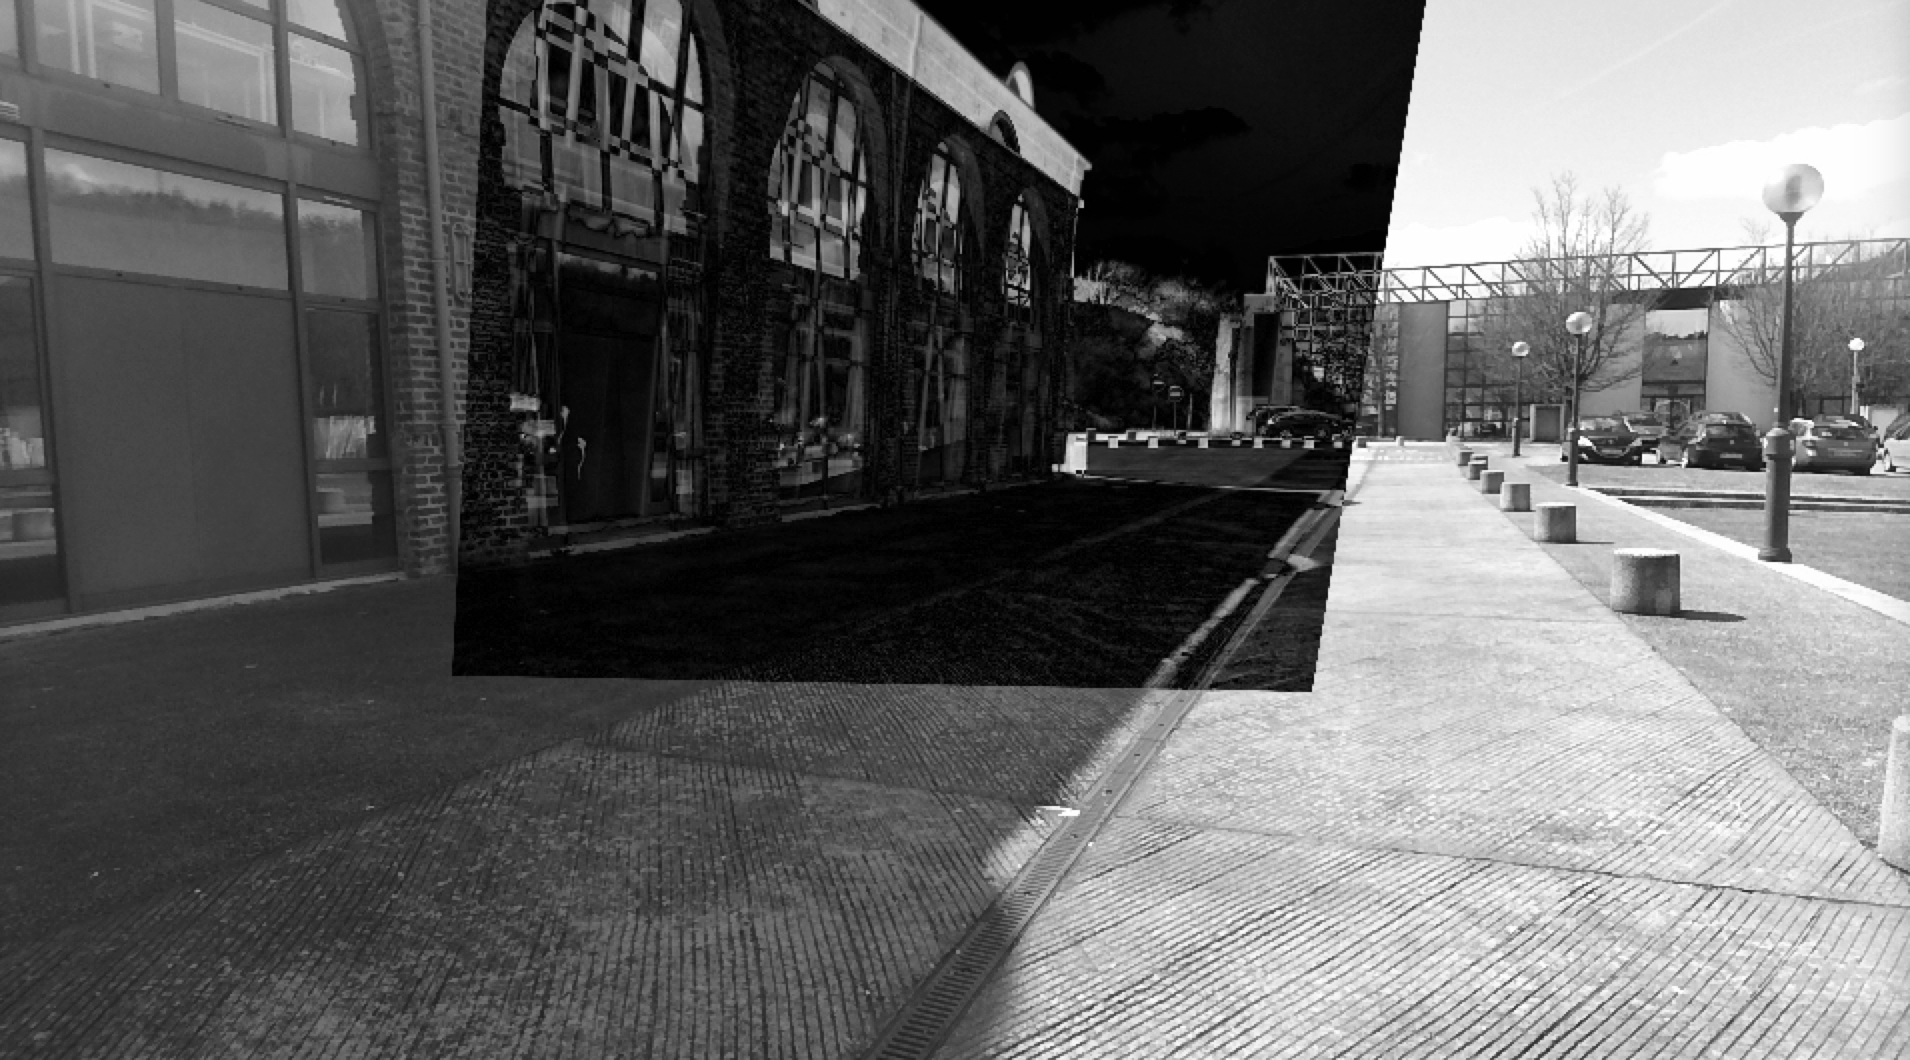
\includegraphics[width=\linewidth]{Figures/Dataset/beforealign.png}
	\end{subfigure}
	\begin{subfigure}{.4\textwidth}
		
		\centering
		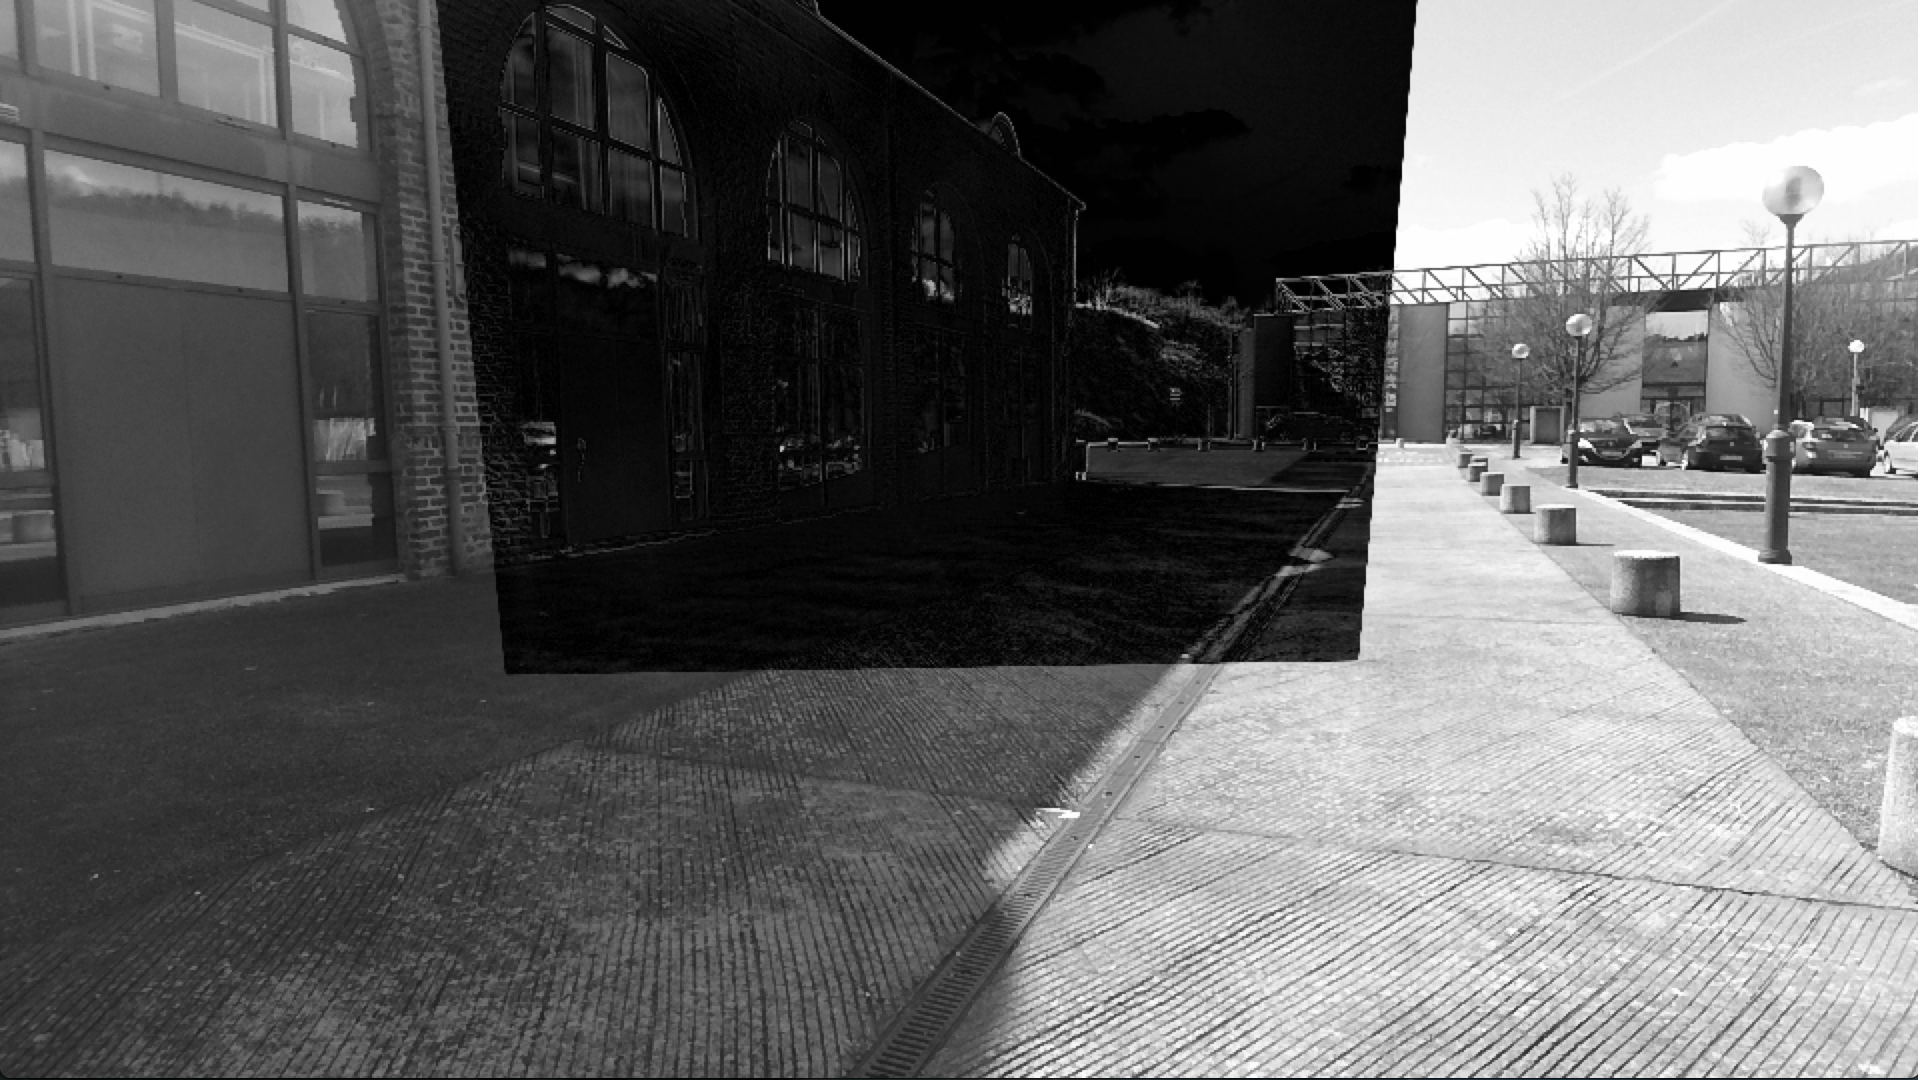
\includegraphics[width=\linewidth]{Figures/Dataset/afteralign.png}
	\end{subfigure}
	\caption{Before and after dense alignment between polarimetric and RGB intensity images.}
	\label{fig:beforeafteralign}
\end{figure}


It is then possible to minimize the function through an iterative process or, in our case, to define an error target $\epsilon$. Indeed, since the starting hypothesis has invalidated the possibility of photometrically comparing the intensity images, we must empirically set an error threshold that will satisfy the alignment needs.
In addition, there is the parameter $Z$ that must be estimated or evaluated using a grid search approach. Finally, as shown in the Figure \ref{fig:beforeafteralign}, dense alignment seems to represent a viable solution. It is however important to mention the computational requirements are high and that this kind of process is heavy. Despite its efficiency, it is a matter of obtaining a tradeoff between a potentially precise alignment and a computation time consistent with the application.
In our dataset construction application, there is no online alignment which does not subject our pipeline to the slowness induced by this kind of process.

\section{Augmentation}\label{aug_4}

Augmentation has a major interest when dealing with a limited amount of data. This procedure allows to generalize the DCNN models and avoid overfitting \cite{DBLP:journals/corr/abs-1712-04621}.
However, this process has been principally designed to increase the population of interpolable modalities, but polarization cannot straightforwardly benefit from it by its nature.

Since the information acquired through a polarimetric sensor is intrinsically dependent on its pose, seeking a transformation without adaptation is invalid.
For these reasons, we have explored the augmentation operations applicable to polarization under any conditions.
Thus, we have estimated the two simple adaptable operations are the rotation and the flipping respectively described in \ref{rot} and \ref{syn}.
Finally, \ref{fin_proc} will be dedicated to the final reproducible procedure to multiply the polarimetric images.

\subsection{Rotation}\label{rot}

Rotation remain a very common operation to increase the number of images in a dataset. In practice it is enough to apply a rotation to the image and a new one is obtained. However, since the polarization information is relative to the camera pose, it is necessary to modify the operation.

The prerequisite for augmentation is to create new realistic images. If we transpose an image rotation to the sensor point of view, this procedure is equivalent to rotating the camera. 
This is where the constraint to polarimetry comes from, since pivoting the sensor means changing the camera pose.
Thus, altering the orientation of the camera changes the organization of the camera's pixel grid as shown in Figure \ref{rottheo}. And the objective is to reorganize these pixels so that the polarization angle regains its physical integrity.

\begin{figure}[h]
	\vspace{0.3cm}
	\centering
	\usetikzlibrary{patterns} % la librairie qui permet de remplir avec des motifs, cf le manuel : https://tex.stackexchange.com/questions/29808/can-i-control-the-density-of-a-pattern-in-tikz

% Pour personnaliser éventuellement les hachures : https://tex.stackexchange.com/questions/29808/can-i-control-the-density-of-a-pattern-in-tikz


% Autre fonction utile : la fonction clip, qui permet de découper une partie de dessin selon une géométrie
%
%
%INCLUDE ONCE

\tikzset{
    hatch distance/.store in=\hatchdistance,
    hatch distance=10pt,
    hatch thickness/.store in=\hatchthickness,
    hatch thickness=0.3pt
}

\makeatletter
\pgfdeclarepatternformonly[\hatchdistance,\hatchthickness]{northeast}
{\pgfqpoint{0pt}{0pt}}
{\pgfqpoint{\hatchdistance}{\hatchdistance}}
{\pgfpoint{\hatchdistance-1pt}{\hatchdistance-1pt}}%
{
    \pgfsetcolor{\tikz@pattern@color}
    \pgfsetlinewidth{\hatchthickness}
    \pgfpathmoveto{\pgfqpoint{0pt}{0pt}}
    \pgfpathlineto{\pgfqpoint{\hatchdistance}{\hatchdistance}}
    \pgfusepath{stroke}
}

\pgfdeclarepatternformonly[\hatchdistance,\hatchthickness]{northwest}
{\pgfqpoint{0pt}{0pt}}
{\pgfqpoint{\hatchdistance}{\hatchdistance}}
{\pgfpoint{\hatchdistance-1pt}{\hatchdistance-1pt}}%
{
    \pgfsetcolor{\tikz@pattern@color}
    \pgfsetlinewidth{\hatchthickness}
    \pgfpathmoveto{\pgfqpoint{\hatchdistance}{0pt}}
    \pgfpathlineto{\pgfqpoint{0pt}{\hatchdistance}}
    \pgfusepath{stroke}
}

\pgfdeclarepatternformonly[\hatchdistance,\hatchthickness]{horizontal}
{\pgfqpoint{0pt}{0pt}}
{\pgfqpoint{\hatchdistance}{\hatchdistance}}
{\pgfpoint{\hatchdistance-1pt}{\hatchdistance-1pt}}%
{
    \pgfsetcolor{\tikz@pattern@color}
    \pgfsetlinewidth{\hatchthickness}
    \pgfpathmoveto{\pgfqpoint{0pt}{0pt}}
    \pgfpathlineto{\pgfqpoint{\hatchdistance}{0pt}}
    \pgfusepath{stroke}
}

\pgfdeclarepatternformonly[\hatchdistance,\hatchthickness]{vertical}
{\pgfqpoint{0pt}{0pt}}
{\pgfqpoint{\hatchdistance}{\hatchdistance}}
{\pgfpoint{\hatchdistance-1pt}{\hatchdistance-1pt}}%
{
    \pgfsetcolor{\tikz@pattern@color}
    \pgfsetlinewidth{\hatchthickness}
    \pgfpathmoveto{\pgfqpoint{0pt}{0pt}}
    \pgfpathlineto{\pgfqpoint{0pt}{\hatchdistance}}
    \pgfusepath{stroke}
}
\makeatother


\begin{center}
\resizebox{\linewidth}{!}{
\begin{tikzpicture}

\draw[pattern=horizontal,pattern color=gray,hatch distance=8pt, hatch thickness = 0.8pt]  (0,1.5) rectangle (1.5,3)node[midway]{$0^\circ$}; % texte avec fond
 \draw[pattern=northwest,pattern color=gray,hatch distance=10pt, hatch thickness = 0.8pt] (1.5,1.5) rectangle (3,3) node[midway]{$45^\circ$};
 \draw[pattern=vertical,pattern color=gray,hatch distance=8pt, hatch thickness = 0.8pt](1.5,0) rectangle (3,1.5)
node[midway]{$90^\circ$};
\draw[pattern=northeast,pattern color=gray,hatch distance=10pt, hatch thickness = 0.8pt]  (0,0) rectangle (1.5,1.5)
node[midway]{$135^\circ$};

\draw (1.5,3.5) node[below]{Base Image};

\begin{scope}[shift={(4,0)}]

\draw[pattern=horizontal,pattern color=gray,hatch distance=8pt, hatch thickness = 0.8pt]  (1.5,1.5) rectangle (3,3)node[midway]{$0^\circ$}; % texte avec fond
 \draw[pattern=northwest,pattern color=gray,hatch distance=10pt, hatch thickness = 0.8pt] (1.5,0) rectangle (3,1.5) node[midway]{$45^\circ$};
 \draw[pattern=vertical,pattern color=gray,hatch distance=8pt, hatch thickness = 0.8pt](0,0) rectangle (1.5,1.5)
node[midway]{$90^\circ$};
\draw[pattern=northeast,pattern color=gray,hatch distance=10pt, hatch thickness = 0.8pt]  (0,1.5) rectangle (1.5,3)
node[midway]{$135^\circ$};

\draw (1.5,3.5) node[below]{Transformed ($+90^\circ$)};

\end{scope}

\begin{scope}[shift={(8,0)}]

\draw[pattern=horizontal,pattern color=gray,hatch distance=8pt, hatch thickness = 0.8pt]  (0,1.5) rectangle (1.5,3)node[midway]{$0^\circ$}; % texte avec fond
 \draw[pattern=northwest,pattern color=gray,hatch distance=10pt, hatch thickness = 0.8pt] (1.5,1.5) rectangle (3,3) node[midway]{$45^\circ$};
 \draw[pattern=vertical,pattern color=gray,hatch distance=8pt, hatch thickness = 0.8pt](1.5,0) rectangle (3,1.5)
node[midway]{$90^\circ$};
\draw[pattern=northeast,pattern color=gray,hatch distance=10pt, hatch thickness = 0.8pt]  (0,0) rectangle (1.5,1.5)
node[midway]{$135^\circ$};

\draw (1.5,3.5) node[below]{Regularized Image};

\end{scope}

\end{tikzpicture}
}
\end{center}


	
	\caption{Illustration of the pixel grid of a rotated DoFP polarimetric camera. }\label{rottheo}
\end{figure}

In Figure \ref{rottheo}, the illustration on the left shows the initial polarizer grid, then directly on the right, the effect of a $90^\circ$ rotation on this same grid.

The illustration on the far right shows the prerequisite for the image to be unaltered. A regularization operation is therefore necessary.

We propose applying a rotation to the image, and, to regularize, to apply an inverse rotation to the polarization angle. Ultimately, it brings back both the physics of the scene while keeping this transformation to create a new valid image.

Let $\theta$ be the rotation angle applied to the camera, $R_\theta$ the rotation operation and $H$ the hue channel of the image (which as a reminder corresponds to the angle of polarization $\alpha$):

\begin{equation}\label{eq:Rot}
H_{\textrm{rotated}} = R_{\theta} (H_{prev} - 2 * \textrm{\Big{.\textbf{1}}}\theta).
\end{equation}



\begin{figure}[h]
	\vspace{0.3cm}
	\centering
	\begin{subfigure}[b]{0.32\linewidth}
		\centering
		\caption*{Base Image}
		
		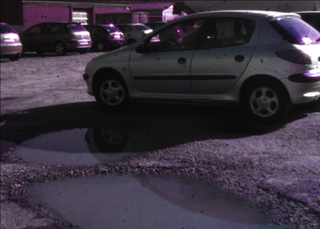
\includegraphics[width=\linewidth]{Figures/Aug/hsl.png}
	\end{subfigure}
	\begin{subfigure}[b]{0.32\linewidth}  
		\centering 
		\caption*{Rotated Image}
		
		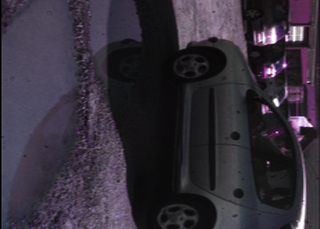
\includegraphics[width=\linewidth]{Figures/Aug/hsl_trans_rot.png}
	\end{subfigure}
	\begin{subfigure}[b]{0.32\linewidth}
		\centering
		\caption*{Regularized Image}
		
		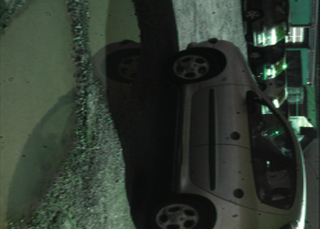
\includegraphics[width=\linewidth]{Figures/Aug/regularized_rot.png}
	\end{subfigure}

	\caption{Step-by-step rotation applied to polarimetric image.}\label{rotreal}
\end{figure}

Since the general idea is to reobtain the viability of the scene physics, this regularization step reorganizing the pixels of the DoFP grid is mandatory. However, as shown in the Figure \ref{rotreal}, this operation impacts the visual of the image. As shown in the Section \ref{rep_pol}, the images are modulated on the HSL model. As a reminder, we indexed the $\alpha$ polarization angle on the Hue channel, or more directly the color. Since the equation \ref{eq:Rot} applies a modification on this channel, then the global hue of the image changes. This is consistent with the fact that the change in pose implies a reorientation of all angles. To guarantee the periodicity of the angle but also to respect the HSL format, an additional modulo step is necessary:
\begin{equation}\label{eq:mod}
H_{final} = H_{transformed} \pmod{360}
\end{equation} 

As a partial conclusion, it is possible to deduce this operation is valid and respects the modality thanks to this visual indicator. In addition, the equation \ref{eq:mod} allows a correct bounding as well as taking advantage of the HSL mode. Thus, any rotation is applicable without altering the information.

In addition, the rotation represent a physically verifiable operation. It does not imply an impossible transformation to the sensor and therefore it is possible to verify the viability of the regularization by performing acquisitions.
As shown in the Figure \ref{proofexper}, this manipulation was performed to physically verify if the polarization information maintained by our equation.

\begin{figure}[h]
	\centering
	\begin{subfigure}[b]{0.3\linewidth}  
		\centering 
		\caption{Acquisition 0$^\circ$}
		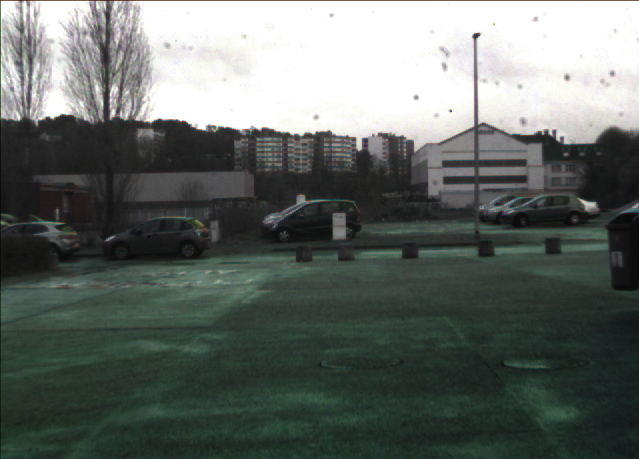
\includegraphics[width=\linewidth]{Figures/Aug/exprimentalTest/phys0.png}
	\end{subfigure}
	\begin{subfigure}[b]{0.3\linewidth}   
		\centering 
		\caption{Acquisition 90$^\circ$}
		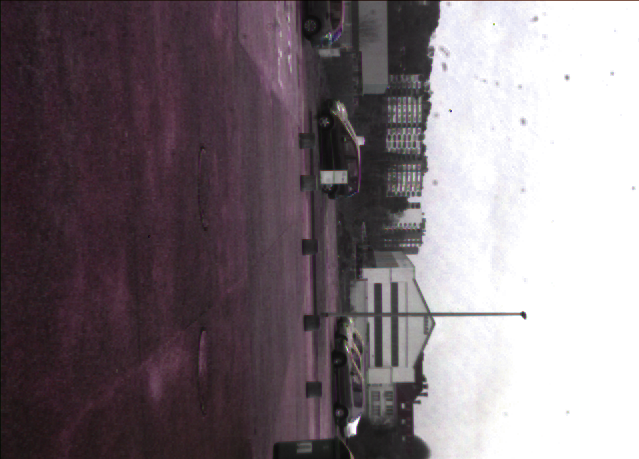
\includegraphics[width=\linewidth]{Figures/Aug/exprimentalTest/phys90.png}
	\end{subfigure}
	\begin{subfigure}[b]{0.3\linewidth}   
		\centering 
		\caption{Augmented 90$^\circ$}
		\includegraphics[width=\linewidth]{Figures/Aug/exprimentalTest/augmented.png}
	\end{subfigure}
	\caption[Experimental validation of rotation process.]{Experimental validation of rotation process.  Images (A) and (B) are acquisitions with physical rotations applied to the camera. Image (C) is the result of augmentation applied to image (A). Note the correct recovery of angle information.
	}\label{proofexper}
\end{figure}

The experimentation consists simply of two acquisitions. One image is captured with the camera oriented normally and a second one with a rotation of 90$^\circ$. We can then perceive the change in hue that this rotation implies. In addition, we can use the non-rotated image and transform it using our process. Thus, we obtain two images: one where the sensor has been physically rotated, and the other that has been artificially rotated.
Subsequently, it is possible to see the shades are approximately the same. A difference is present, but this is due to the parallax effect (imperfect rotation around the depth axis) and since the sensor used is not square. Nevertheless, this experiment shows the validity of the rotation process applied to polarimetry.

In conclusion, this experimental proof validates the rotation process and its associated regularization equation.



\subsection{Symmetry}\label{syn}

Symmetry is another frequently used transformation for augmentation. It allows "disorienting" the algorithms so that they do not get used to positional criteria, much like rotation.
The significant drawback of this transformation is that, unlike rotation, it is not physically verifiable. It goes without saying it is impossible to reverse the scene or to turn the sensor on itself.
This is why we have developed a method to express the impact of this operation and thus validate it.

\begin{figure}[h]
	\centering
	\begin{subfigure}[b]{0.29\linewidth}
		\centering
		\caption*{\footnotesize Base Image}
		
		\includegraphics[width=\linewidth]{Figures/Aug/grad.jpg}
	\end{subfigure}
	\begin{subfigure}[b]{0.29\linewidth}  
		\centering 
		\caption*{\footnotesize Flipped Image}
		
		\includegraphics[width=\linewidth]{Figures/Aug/flipped.jpg}
	\end{subfigure}
	\begin{subfigure}[b]{0.29\linewidth}
		\centering
		\caption*{\footnotesize Regularized Image}
		
		\includegraphics[width=\linewidth]{Figures/Aug/grad.jpg}
	\end{subfigure}
	\caption[Illustration of the flipping procedure.]{Illustration of the flipping procedure. From left to right, the base image, a flipped image and the regularized image}\label{flipreadtheo}
\end{figure}
The figure \ref{flipreadtheo} shows a circle separated into two halves.
This illustration is specific because each point of the circle in the image represents the corresponding angle with the center as reference.
If we consider only the top of the left circle, from left to right, we have a circular gradient ranging from 180 degrees to 0 degrees. Therefore, this image represents the full range of possible linear polarization angles in an image.
Knowing that the image hue channel is periodic at 360 degrees, the reversal consists of inverting the axis selected for the transformation.
Taking advantage of the periodicity of the angle and the selected format, then the transformation can be performed as follows:

\begin{equation}\label{eq:flip}
H_{\textrm{flipped}} = -H_{prev}.
\end{equation} 

Clearly, the physical operation of flipping is operated on the image in addition to regularization.
Thanks to the equation \ref{eq:mod} in addition to equation \ref{eq:flip}, we possess the possibility to use the representation mode to our advantage. This operation makes the format valid and thus, the accumulation of these two manipulations is necessary to verify the simulation proposed in figure \ref{flipreadtheo}.
Finally, the equation has this double role of regularization for symmetry and buffer to guarantee the validity of the color space.


\begin{figure}[h]
	\centering

	\begin{subfigure}[b]{0.32\linewidth}
		\centering
		\caption*{Base Image}
		
		\includegraphics[width=\linewidth]{Figures/Aug/hsl_flip.png}
	\end{subfigure}
	\begin{subfigure}[b]{0.32\linewidth}  
		\centering 
		\caption*{Flipped Image}
		
		\scalebox{-1}[1]{\includegraphics[width=\linewidth]{Figures/Aug/hsl_flip.png}}
	\end{subfigure}
	\begin{subfigure}[b]{0.32\linewidth}
		\centering
		\caption*{Regularized Image}
		
		\includegraphics[width=\linewidth]{Figures/Aug/regularized_flipped.png}
	\end{subfigure}
	
	\caption[Flipping operation on real image and impact.]{Flipping operation on real image and impact. From left to right, initial image, the flipped image and the regularized image.}\label{flipread}
\end{figure}

It is then possible to perform these transformations on real images as shown in the figure \ref{flipread}.
Since it is impossible to physically observe this kind of transformation, the visual hue indexer will be the sole indicator of an integral transformation. Despite this, it is equally possible to check if the hue is well "inverted" by checking on the HSL representation space (shown in figure \ref{fig:hslrgb}) if the colors are properly symmetrical.

In conclusion, we note symmetry is another valid augmentation possibility to obtain realistic images of polarization thanks to our regularization process.


\subsection{Final procedure}\label{fin_proc}

In this part the final procedure of augmentation will be explained, but first of all a point must be addressed: what happens to the other channels.
Indeed, in the two previous parts on the different transformations, only the angle was modified. This can be explained by the invariance of the other two channels, the degree of polarization and the intensity, with respect to the pose.
The observation is simple, the reflection strength or the texture does not change according to the pose, such as, a reflective object remains reflective regardless of the camera orientation. Similarly, the texture is unaffected by a change in pose similarly to usual colorimetric image processing.
Thus, we conclude only the angle must undergo regularization operations while the other channels will only be affected by the rotation or flipping type transformation.



\begin{figure}[h]
	\centering
	\includegraphics[width=.7\linewidth]{Figures/Aug/diagram-20190220.png}
	%\input{aug.tex}
	\caption[Illustration of the augmentation per image procedure.]{Illustration of the augmentation per image procedure. This process is repeated for each image in the original dataset to obtain a consistent large dataset. Then, the entire set of augmented images is shuffled.}\label{augment}
\end{figure}

This observation allowing to conclude on the augmentation pipeline, it is then possible to define the final process to augment the dataset.
Augmentation is typically composed of multiple operations performed simultaneously according to probabilistic or empirical rules. 
We therefore propose, with our transformations, to compose in the same way. Thus, we have the ability to cumulate rotation and flipping, at different increments or orientation.
As shown in the figure \ref{augment}, from a polarimetric image, we convert it to HSL as explained in Section \ref{rep_pol}. At that point in time, the image is randomly rotated by increments of 5$^\circ$ and flipped according to an empirically fixed probability. To complete the augmentation, our algorithm checks the uniqueness of the image to prevent redundancies and then converts these images in RGB format as expressed in Section \ref{rep_pol}.


At the end of this augmentation pipeline\footnote{Available at: \url{https://github.com/BlanchonMarc/P_Augmentor}}, starting from a unique image, it is possible to obtain $N$ physically correct polarimetric images. Following our numerous experiments, we concluded that 11 images generated with a unique image (i.e. 12 images in total as shown in the illustration) was sufficient to obtain enough images. 


Finally, implementing all these manipulations, we have proposed a new pipeline to perform augmentation operations on a physical-based modality, polarimetry.


\section{Network architectures}\label{net_4}

As a usefulness proof of polarization for the understanding of urban areas, we propose performing a benchmark comparing colorimetry and polarimetry, but also to approve the augmentation method presented in Section \ref{aug_4}.

Since one of the most widespread understanding applications is DL-based PwSS, we propose to perform this quantitative and qualitative study using proven architecture in literature.

\subsection{SegNet}\label{segnet_sec}

SegNet\cite{DBLP:journals/corr/BadrinarayananH15}, shown in Figure \ref{seg-arch}, is a simple architecture composed of an encoder and a decoder. Designed for scene segmentation and widely used with "city/road" datasets.  This network is not considered the state of the art but rather a pioneer in the field of PwSS.  It is notable for its small number of layers and simple composition (shown in the table \ref{tab:segnet}). 

\begin{figure}[h]
	\centering
	\includegraphics[width=\linewidth]{Figures/master-thesis/segnet.png}
	%\input{aug.tex}
	\caption{Illustation of SegNet architecture.}\label{seg-arch}
\end{figure}

The chief idea behind the emergence of this network as a point of comparison between RGB and Polarimetry is that it is not especially necessary to use overly complex networks. Indeed, the approach here is not principally to observe efficient results but to compare in the most unbiased way the ability to appreciate the scenes through different modalities. 
Thus, through this network, it is possible, with a simple encoder-decoder architecture, to focus on the modality and not on the performances that the network could infuse.


\begin{table}[h]
	\caption{Detailed SegNet architecture.}
	\centering
	\begin{adjustbox}{width=1\textwidth}
		\begin{tabular}{| c | c  c  c  c  c || c | c  c  c  c  c |}
			
			\toprule
			\multicolumn{6}{|c||}{\textbf{Encoder}}
			&
			\multicolumn{6}{|c|}{\textbf{Decoder}} \\\cline{1-6}\cline{7-12} 
			&\textbf{Type}&\textbf{Kernel}&\textbf{Padding}&\textbf{Stride}&\textbf{Output Depth}& &\textbf{Type}&\textbf{Kernel}&\textbf{Padding}&\textbf{Stride}&\textbf{Output Depth}\\\cline{1-6}\cline{7-12} 
			
			&conv1&3x3&1&1&Depth Image& &conv14&3x3&1&1&512\\
			\textbf{Block1}&conv2&3x3&1&1&64&\textbf{Block1d}&conv15&3x3&1&1&512\\
			& & & & & & &conv16&3x3&1&1&512\\\cline{1-6}\cline{7-12}
			
			&conv3&3x3&1&1&64& &conv17&3x3&1&1&512\\
			\textbf{Block2} &conv4&3x3&1&1&128&\textbf{Block2d}&conv18&3x3&1&1&512\\
			& & & & & & &conv19&3x3&1&1&256\\\cline{1-6}\cline{7-12}
			
			&conv5&3x3&1&1&128& &conv20&3x3&1&1&256\\
			\textbf{Block3}&conv6&3x3&1&1&256&\textbf{Block3d}&conv21&3x3&1&1&256\\
			&conv7&3x3&1&1&256& &conv22&3x3&1&1&126\\\cline{1-6}\cline{7-12}
			
			&conv8&3x3&1&1&256& &conv23&3x3&1&1&126\\
			\textbf{Block4}&conv9&3x3&1&1&512&\textbf{Block4d}&conv24&3x3&1&1&64\\
			&conv10&3x3&1&1&512& & & & & & \\\cline{1-6}\cline{7-12}
			
			&conv11&3x3&1&1&512& &conv25&3x3&1&1&64\\
			\textbf{Block5}&conv12&3x3&1&1&512&\textbf{Block5d}&conv26&3x3&1&1&Desired Depth\\
			&conv13&3x3&1&1&512& & & & & & \\
			\bottomrule
		\end{tabular}
	\end{adjustbox}
	\vspace{0.5ex}
	\label{tab:segnet}
\end{table}


\subsection{DeepLab V3+}\label{deeplab_sec}

DeepLab v3+\cite{chen2017rethinking}, shown in Figure \ref{deeplab-fig}, is much more advanced compared to SegNet. Indeed, its complex design composed of atrous convolution and ASPP (these two concepts are explained in the Chapter) is much more powerful than the previous architecture. 
\begin{figure}[h]
	\centering
	\includegraphics[width=\linewidth]{Figures/DL/deeplab-arch.png}
	%\input{aug.tex}
	\caption[Illustation of DeepLab V3+ architecture.]{Illustation of DeepLab V3+ architecture. Schematic borrowed from \cite{chen2017rethinking}.}\label{deeplab-fig}
\end{figure}


The use of such a network is motivated by the need to quantify the utility of the augmentation in favorable situations. Indeed, by implementing a complex architecture, it is possible to benefit the learning of complex features and in this case, the physical validity of polarimetry. 
In this manner, it will be possible to quantify the usefulness and/or the necessity of the augmentation.



\section{Experiments}\label{exp_4}

The experiments conducted allow two independent scopes.


On one hand, a series of experiments is focused on the differences of modalities. The prime goal of this set is to demonstrate the interest of polarization over colorimetry. The idea is to prove that with the same comparison method, a alternative form of information sustains a considerable interest for some fields. Therefore, without needing to unnecessarily increase the complexity of the processing cores, it is possible to reach satisfactory results.


In a second step, we propose to investigate the usefulness of an augmentation adapted to a physics-based modality. Here, in order for the algorithm to grasp maximum advantage of the available information (valid or invalid), we use a state-of-the-art DCNN. 

\subsection{Modality-based Comparison}

In this section, our proposal is to compare the modalities on the same basis, using aligned images, representing the same scenes.
We manipulate the non-augmented images from PolaBot (see Section \ref{data_pol}) and the network presented in Section \ref{segnet_sec}.

The images presented to the network show urban scenes that are conducive to reflection. As a reminder, we assume a large number of objects are reflective in urban areas such as: cars, windows or wet roads.
Thus, to highlight the respective capabilities of the networks trained jointly with colorimetry and polarimetry, the images were manually annotated with eight particular classes.
These eight classes designed for autonomous robotics are: Buildings (gray), Car (red), Road (orange), Sky (green), Water (blue), Window (light yellow), None (white) and Unlabeled (black). These classes are clearly differentiated by their segmented color and were determined for their interest in complex areas but also because they can lead to confusion with standard sensors. Also, the None class represents all the areas that have been judged uninterestingly for our comparison (e.g. trees, sidewalks,...) and the Unlabeled class comes from manual annotation errors.


Therefore, a simple metric, allowing an explicit comparison, was chosen. Indeed, the accuracy per class has been defined as:


\begin{equation}
\textrm{Accuracy}_C = \frac{\sum \; ^pP_C}{\sum \; ^gP_C},
\end{equation}

with C the class, $^pP_C$ the correctly predicted pixel of the class C and $^gP_C$ the ground truth pixel of class C.

For the training procedure, the construction of the dataset (explained in previous section) allows for pre-training and therefore the use of transfer learning\cite{torrey2010transfer,pan2009survey} to help convergence and benefit from efficient previous training. Therefore, both networks have been pre-trained using VGG16. 
This process, in addition to being advantageous, will allow us both to verify if the HSL to RGB approach is valid but also to see the adaptation capabilities of the network to a physics-based modality although pre-trained with colorimetry.

\subsubsection{Results}

Since the training procedure was identical in the hyperparameters as well as in the order of appearance of the images, it is possible to quantitatively compare the results between the two modalities.


As shown in Figure \ref{fig:resultspwss}, the qualitative results seem almost identical. However, when analyzing Table \ref{AccDiff}, a significant difference appears in favor of polarization. 

\begin{figure}[!htb]
\captionsetup{width=\linewidth}	
\begin{minipage}{0.48\textwidth}
		\captionsetup{width=.8\linewidth}
		\centering
		\begin{subfigure}[b]{0.3\linewidth}
			\reflectbox{\rotatebox[origin=c]{180}{\includegraphics[width=\linewidth]{Figures/VISAPP/1pred.png}}}
		\end{subfigure}
		\begin{subfigure}[b]{0.3\linewidth}
			\reflectbox{\rotatebox[origin=c]{180}{\includegraphics[width=\linewidth]{Figures/VISAPP/1gt.png}}}
		\end{subfigure}
		\begin{subfigure}[b]{0.3\linewidth}
			\reflectbox{\rotatebox[origin=c]{180}{\includegraphics[width=\linewidth]{Figures/VISAPP/1int.png}}}
		\end{subfigure}\\
		\begin{subfigure}[b]{0.3\linewidth}
			\includegraphics[width=\linewidth]{Figures/VISAPP/49pred.png}
		\end{subfigure}
		\begin{subfigure}[b]{0.3\linewidth}
			\includegraphics[width=\linewidth]{Figures/VISAPP/49gt.png}
		\end{subfigure}
		\begin{subfigure}[b]{0.3\linewidth}
			\includegraphics[width=\linewidth]{Figures/VISAPP/2int.png}
		\end{subfigure}\\
		\begin{subfigure}[b]{0.3\linewidth}
			\reflectbox{\rotatebox[origin=c]{180}{\includegraphics[width=\linewidth]{Figures/VISAPP/313pred.png}}}
		\end{subfigure}
		\begin{subfigure}[b]{0.3\linewidth}
			\reflectbox{\rotatebox[origin=c]{180}{\includegraphics[width=\linewidth]{Figures/VISAPP/313gt.png}}}
		\end{subfigure}
		\begin{subfigure}[b]{0.3\linewidth}
			\reflectbox{\rotatebox[origin=c]{180}{\includegraphics[width=\linewidth]{Figures/VISAPP/5int.png}}}
		\end{subfigure}		
		\subcaption{Polarimetry PwSS qualitative results.}
		\label{fig:polares}	
\end{minipage}
\hfill
\begin{minipage}{0.48\textwidth}
		\captionsetup{width=\linewidth}	
		\centering
		\begin{subfigure}[b]{0.3\linewidth}
			\reflectbox{\rotatebox[origin=c]{180}{\includegraphics[width=\linewidth]{Figures/VISAPP/1predrgb.png}}}
		\end{subfigure}
		\begin{subfigure}[b]{0.3\linewidth}
			\reflectbox{\rotatebox[origin=c]{180}{\includegraphics[width=\linewidth]{Figures/VISAPP/1gtrgb.png}}}
		\end{subfigure}
		\begin{subfigure}[b]{0.3\linewidth}
			\reflectbox{\rotatebox[origin=c]{180}{\includegraphics[width=\linewidth]{Figures/VISAPP/11int.png}}}
		\end{subfigure}\\
		\begin{subfigure}[b]{0.3\linewidth}
			\reflectbox{\includegraphics[width=\linewidth]{Figures/VISAPP/55predrgb.png}}
		\end{subfigure}
		\begin{subfigure}[b]{0.3\linewidth}
			\reflectbox{\includegraphics[width=\linewidth]{Figures/VISAPP/55gtrgb.png}}
		\end{subfigure}
		\begin{subfigure}[b]{0.3\linewidth}
			\reflectbox{\includegraphics[width=\linewidth]{Figures/VISAPP/12int.png}}
		\end{subfigure}\\
		\begin{subfigure}[b]{0.3\linewidth}
			\reflectbox{\rotatebox[origin=c]{180}{\includegraphics[width=\linewidth]{Figures/VISAPP/25predrgb.png}}}
		\end{subfigure}
		\begin{subfigure}[b]{0.3\linewidth}
			\reflectbox{\rotatebox[origin=c]{180}{\includegraphics[width=\linewidth]{Figures/VISAPP/25gtrgb.png}}}
		\end{subfigure}
		\begin{subfigure}[b]{0.3\linewidth}
			\reflectbox{\rotatebox[origin=c]{180}{\includegraphics[width=\linewidth]{Figures/VISAPP/15int.png}}}
		\end{subfigure}
		\subcaption{Colorimetry PwSS qualitative results.}
		\label{fig:rgbres}	
\end{minipage}

\caption[Qualitative results comparing colorimetry and polarimetry with identical scenes.]{Qualitative results comparing colorimetry and polarimetry with identical scenes. For both the montages, respectively from left to right the images are: prediction, ground truth and input.}\label{fig:resultspwss}
\end{figure}



\begin{table}[h]
	\centering
	\caption{PwSS quantitative results comparing polarimetry and RGB.}
	\label{AccDiff}
	\resizebox{1\textwidth}{!}{
	\begin{tabular}{c|c|c|c|c|c|c|c||c|c|}
		\cline{2-9}
		& \textcolor{sky}{Sky} & \textcolor{water}{Water} & \textcolor{windows}{Windows} & \textcolor{road}{Road} & \textcolor{car}{Cars} & \textcolor{buildings}{Building} & \textcolor{none}{None} & Mean \\ \cline{2-8} \hline
		\multicolumn{1}{|c|}{Polarimetry} & 75.34 \%                    & 75.70 \%                      & 82.85 \%                       & 77.82 \%                     & 71.40 \%                    & 87.69 \%                         & 78.95 \% & 78.54 \%                    \\ \hline
		\multicolumn{1}{|c|}{RGB} & 89.57 \% & 78.61 \% & 44.50 \% & 78.45 \% & 48.48 \% & 67.84 \% & 83.4 \% & 69.83 \%                    \\ \hline \hline
		\multicolumn{1}{|c|}{Difference}  & -14.23\% & -3.51 \% & 38.35 \% & -0.63 \% & 22.92 \% & 19.85 \% & -4.45 \%  & 8.71 \%                  \\ \hline
	\end{tabular}}
	
\end{table}

Indeed, the accuracy per class shows with a network trained with polarimetric information, windows, cars and buildings are recognized in a better way. Moreover, the mean column shows a significant improvement compared to the identical algorithm using colorimetry.


\subsubsection{Discussion}

After numerous experiments and despite a fair comparison, the polarization-based approach seems to be more appropriate for the PwSS of complex urban scenes compared to colorimetry. Indeed, the use of polarization as a disciminant factor upstream of the network shows that for certain specificities, this information is more robust. 
It should be noted that the dataset was designed to highlight these DCNN behaviors which may partially explain the increased performance. Nevertheless, despite these advantages, polarization has proved its value. However, there is up until now an issue of data availability and consequently, the lack of consistent datasets.

This experiment also showed that DCNNs was able to adapt to supplementary information and that we could use transfer learning to rely only on fine-tuning. Moreover, the two methods compared having identical training, the learning on polarization emphasized a faster convergence. 

On the other hand, in the wrong direction, polarization was supposed to have a significant advantage over the Sky class since it is polarized. One possible explanation is the color makes it easy to discern the blue of the sky. Indeed, after experimentation, the dataset was found to be biased by this fact and in every image showing sky, it was blue. Thus, this is in our opinion the most plausible way to explain this performance which exceeds that of the polarization-based network.

To conclude this discussion, it is significant to note that polarization offers a substantial advantage for certain applications and especially for recognizing areas prone to reflection. Regrettably, the data is relatively rare and therefore not widely available. Nevertheless, through these experiments, it has been shown that a network is not only capable of learning from physics-based images but also that it is beneficial. Even with limited data, the comparisons emphasized the increased capabilities when the learning was conducted with this unconventional data.

\subsection{Augmentation-based Comparison}\label{abc}

Now that it has been established, that polarization-based algorithms tends to show increased performance in complex urban areas; this section will allow a study of the augmentation and its impact.
Indeed, the key idea is to show the interest of increasing the polarimetric image dataset by using the physics-friendly transforms established in section \ref{aug_4}.
Hence the use of an efficient network theoretically allowing a deeper use of the physical information of polarization.
The concept is to check if the augmentation is valid and its impact on the results. Thus, the experiment will be carried out using three different approach involving dataset: one will be not augmented, one augmented without using the regularization equations and a last implementing the augmentation presented in section \ref{aug_4}.
This approach allows a reliable comparison but also emphasizes the importance and even the necessity of an approach adapted to the modality.

\textbf{Encouraging segmented areas' expansion. } Usually, pixel segmentation techniques are discriminated using a simple loss chosen for its gradient behavior in logistic regression similar to the squared error loss for Linear regression. Indeed, the Cross entropy loss (CEL) allows to classify using probabilities and compare an outcome with a reality.
The multi-class CEL is defined as:

\begin{equation}
	CEL(x,c) = -log\Big( \frac{exp(x[c])}{\sum_j exp(x[j])} \Big) = -x[c] + log\Big( \sum_j exp(x[j]) \Big).
\end{equation}

While this feature is efficient, it tends to encourage pixel accuracy but neglects object logic. The fact is that the areas to be segmented are often plain surfaces and -outside of occlusion- do not have different classes. Thus, some applications, particularly medical imaging, opt for the use of the S\o rensen-Dice index (SDI). This one allows to encourage the propagation of a class and favors the fullness of the zones rather than considering only the pixel space. One could say SDI brings a more semantic dimension. This loss is defined as:

\begin{equation}
SDI =\frac{ \sum^{N}_{c} 1 - \frac{2 | X_c \cap Y_c|}{|X_c| + |Y_c|}}{N},\label{eq_dice}
\end{equation}

with  $X$  the label, $Y$ the prediction, $c$ the class and $N$ the number of classes. Since classes are unequally represented in the dataset, this metric allows an equal valuation of each of them unlike other losses.
Therefore, we will use the S\o rensen-Dice index for the training of the different networks since it allows us to obtain more satisfactory results semantically speaking.

\textbf{Metrics. }To effectively compare the diverse approaches and to evaluate the impact of the different augmentation methods, a comprehensive range of metrics were selected.
To effectively compare the different approaches and evaluate the impact of the different augmentation methods, a extensive range of metrics, defined in Appendix \ref{AppendixB}, has been selected. Thus, the \textit{IoU} was selected to quantify the overlap of the segmented areas with respect to the ground truth, the \textit{recall} and the \textit{precision} to measure respectively the consistency and the relevance of the segmentation. In addition, we chose to measure \textit{specificity} since it quantifies the ability to select and remove bad classes. This last metric allows us to verify if the segmentation is efficiently performed by zone and therefore SDI is meaningful for the application.



\subsubsection{Results}

As previously specified, three different DeepLab v3+ networks were trained with three different derivatives of the Polabot dataset.
These three networks will be named:

\begin{itemize}
	\item \emph{None:} for Polabot without any augmentation.
	\item \emph{Standard:} for Polabot augmented but without polarization angle regularization.
	\item \emph{Regularized:} for Polabot augmented and aggregated with the regularization presented in Section \ref{aug_4}.
\end{itemize}

The Standard or Regularized augmentation are both identical in the transformations oapplied n the images. This procedure, whether regularized or not, allows to obtain 2136 images from 178 (i.e. a 12/1 ratio).
In addition, an evaluation was performed based on whether or not the xception subnetworks were pre-trained using provided model\footnote{\url{https://data.lip6.fr/cadene/pretrainedmodels/}}.

As a recall, the scenes correspond to urban areas with seven different classes:

	\mbox{\textit{Road} (\textcolor{road}{dark yellow/orange})}, \textit{Buildings} (\textcolor{buildings}{grey}), \textit{Cars} (\textcolor{car}{red}), \textit{Water} (\textcolor{water}{blue}), \textit{Windows} (\textcolor{windows}{light yellow}), \textit{Sky} (\textcolor{sky}{green}) and \textit{None} (\textcolor{none}{light grey}).

\begin{figure}[h]
	\centering
	\begin{subfigure}[b]{0.3\linewidth}
		\centering
		\includegraphics[width=\linewidth]{Figures/Aug/NA1/selected_images/overlayed/over0.png}
	\end{subfigure}
	\begin{subfigure}[b]{0.3\linewidth}  
		\centering 
		\includegraphics[width=\linewidth]{Figures/Aug/BA1/selected_images/overlayed/over0.png}
	\end{subfigure}
	\begin{subfigure}[b]{0.3\linewidth}  
		\centering 
		\includegraphics[width=\linewidth]{Figures/Aug/CA1/selected_images/overlayed/over0.png}
	\end{subfigure}
	\vskip\baselineskip
	\begin{subfigure}[b]{0.3\linewidth}  
		\centering 
		\includegraphics[width=\linewidth]{Figures/Aug/NA2/selected_images/overlayed/over0.jpg}
	\end{subfigure}
	\begin{subfigure}[b]{0.3\linewidth}  
		\centering 
		\includegraphics[width=\linewidth]{Figures/Aug/BA2/selected_images/overlayed/over0.jpg}
	\end{subfigure}
	\begin{subfigure}[b]{0.3\linewidth}  
		\centering 
		\includegraphics[width=\linewidth]{Figures/Aug/CA2/selected_images/overlayed/over0.jpg}
	\end{subfigure}
	\caption[Illustration of the diverse segmentation results obtained with different augmentation methods.]{Illustration of the diverse segmentation results obtained with different augmentation methods. The top line shows results for DeepLab v3+ network not pre-trained, and the bottom line the results with a pre-trained network. From left to right are presented predictions from networks trained with: un-augmented dataset, standarly augmented dataset and augmented dataset following our procedure. The four most representative segmented classes here are: \textit{Road} (\textcolor{road}{dark yellow/orange}), \textit{Cars} (\textcolor{car}{red}), \textit{Sky} (\textcolor{sky}{light green}) and \textit{None} (\textcolor{none}{light grey}). %In those images, some areas are badly segmented as windows (light yellow).
	}
	\label{comp1}
	\vspace{-0.25cm}
\end{figure}
As shown in Figure\ref{comp1}, for a same scene, 6 estimates are then proposed by the benchmark.



\begin{figure}[h]
	\centering
	
	\begin{subfigure}[b]{0.18\linewidth}   
		\centering 
		\includegraphics[width=\linewidth]{Figures/Aug/labels/overlayed/over1205.png}
	\end{subfigure}
	\begin{subfigure}[b]{0.18\linewidth}
		\centering
		\includegraphics[width=\linewidth]{Figures/Aug/labels/overlayed/over4427.png}
	\end{subfigure}
	\begin{subfigure}[b]{0.18\linewidth}  
		\centering 
		\includegraphics[width=\linewidth]{Figures/Aug/labels/overlayed/over4981.png}
	\end{subfigure}
	\begin{subfigure}[b]{0.18\linewidth}   
		\centering 
		\includegraphics[width=\linewidth]{Figures/Aug/labels/overlayed/over5142.png}
	\end{subfigure}
	\begin{subfigure}[b]{0.18\linewidth}   
		\centering 
		\includegraphics[width=\linewidth]{Figures/Aug/labels/overlayed/over5426.png}
	\end{subfigure}
	
	
	\vspace{0.1cm}
	
	
	\begin{subfigure}[b]{0.18\linewidth}   
		\centering 
		\includegraphics[width=\linewidth]{Figures/Aug/NA2/selected_images/overlayed/over1205.jpg}
	\end{subfigure}
	\begin{subfigure}[b]{0.18\linewidth}
		\centering
		\includegraphics[width=\linewidth]{Figures/Aug/NA2/selected_images/overlayed/over4427.jpg}
	\end{subfigure}
	\begin{subfigure}[b]{0.18\linewidth}  
		\centering 
		\includegraphics[width=\linewidth]{Figures/Aug/NA2/selected_images/overlayed/over4981.jpg}
	\end{subfigure}
	\begin{subfigure}[b]{0.18\linewidth}   
		\centering 
		\includegraphics[width=\linewidth]{Figures/Aug/NA2/selected_images/overlayed/over5142.jpg}
	\end{subfigure}
	\begin{subfigure}[b]{0.18\linewidth}   
		\centering 
		\includegraphics[width=\linewidth]{Figures/Aug/NA2/selected_images/overlayed/over5426.jpg}
	\end{subfigure}
	
	\vspace{0.1cm}  
	
	\begin{subfigure}[b]{0.18\linewidth}   
		\centering 
		\includegraphics[width=\linewidth]{Figures/Aug/BA2/selected_images/overlayed/over1205.jpg}
	\end{subfigure}
	\begin{subfigure}[b]{0.18\linewidth}
		\centering
		\includegraphics[width=\linewidth]{Figures/Aug/BA2/selected_images/overlayed/over4427.jpg}
	\end{subfigure}
	\begin{subfigure}[b]{0.18\linewidth}  
		\centering 
		\includegraphics[width=\linewidth]{Figures/Aug/BA2/selected_images/overlayed/over4981.jpg}
	\end{subfigure}
	\begin{subfigure}[b]{0.18\linewidth}   
		\centering 
		\includegraphics[width=\linewidth]{Figures/Aug/BA2/selected_images/overlayed/over5142.jpg}
	\end{subfigure}
	\begin{subfigure}[b]{0.18\linewidth}   
		\centering 
		\includegraphics[width=\linewidth]{Figures/Aug/BA2/selected_images/overlayed/over5426.jpg}
	\end{subfigure}
	
	\vspace{0.1cm} 
	
	
	\begin{subfigure}[b]{0.18\linewidth}   
		\centering 
		\includegraphics[width=\linewidth]{Figures/Aug/CA2/selected_images/overlayed/over1205.jpg}
	\end{subfigure}
	\begin{subfigure}[b]{0.18\linewidth}
		\centering
		\includegraphics[width=\linewidth]{Figures/Aug/CA2/selected_images/overlayed/over4427.jpg}
	\end{subfigure}
	\begin{subfigure}[b]{0.18\linewidth}  
		\centering 
		\includegraphics[width=\linewidth]{Figures/Aug/CA2/selected_images/overlayed/over4981.jpg}
	\end{subfigure}
	\begin{subfigure}[b]{0.18\linewidth}   
		\centering 
		\includegraphics[width=\linewidth]{Figures/Aug/CA2/selected_images/overlayed/over5142.jpg}
	\end{subfigure}
	\begin{subfigure}[b]{0.18\linewidth}   
		\centering 
		\includegraphics[width=\linewidth]{Figures/Aug/CA2/selected_images/overlayed/over5426.jpg}
	\end{subfigure}
	
	\caption[Examples of segmentation results according to the augmentation methods.]{Examples of segmentation results according to the augmentation methods. From top to bottom are present the ground-truth, then consecutively the results from model with pre-training with: no augmentation, standard augmentation and regularized augmentation.}
	\label{figres_aug}
\end{figure}

It is then possible to extract a range of images from the test dataset which is a video sequence comprised of 8,049 images acquired at a frequency of 10Hz sharing many characteristics with the training dataset.
Figure \ref{figres_aug}, shows a comprehensive panel of images representative of the results obtained from the various trainings.




\renewcommand{\arraystretch}{1.5}
\begin{table}[h]
	\centering
	
	\caption[Quantitative evaluation of augmentation procedures.]{Quantitative evaluation of augmentation procedures.Impact of the augmentation procedure on DeepLabV3+ network. Specific classes have been highlighted in relation to the robotic application to witness the obstacle-wise performance. Due to the limited training, \textit{Buildings} are almost undetected. For this reason, the averages denoted $\backslash B$ exclude the \textit{Buildings} class from the calculation. }\label{metriques}
	\large \center
	\resizebox{\textwidth}{!}{%
		\begin{tabular}{c|c|ccccc|ccccc|c|c}
			\multirow{2}{*}{\textbf{Augmentation}} & \multirow{2}{*}{\textbf{PreTraining}} & \multicolumn{5}{c|}{\textbf{IoU (\%)}}                                         & \multicolumn{5}{c|}{\textbf{Recall (\%)}}                                      & \multirow{2}{*}{\textbf{Precision (\%)}} & \multirow{2}{*}{\textbf{Specificity (\%)}} \\ \cline{3-12}
			&                                       & \textcolor{water}{@water}        & \textcolor{windows}{@windows}      & \textcolor{car}{@cars}         & Mean          & Mean $\backslash B$ & \textcolor{water}{@water}        & \textcolor{windows}{@windows}      & \textcolor{car}{@cars}         & Mean          & Mean $\backslash B$ &                                          &                                                            \\ \hline
			\multirow{2}{*}{None}                  & No                                    & 40.0          & 20.6          & 20.8          & 30.5          & 32.2           & 35.2          & 15.8          & 22.5          & \textbf{50.9} & 50.0           & 50.0                                     & 89.6                                                                           \\
			& Yes                                   & 54.0          & 10.3          & 43.46         & 33.5          & 34.8           & \textbf{42.4 }         & 15.3          & 57.4          & 43.3          & 50.3           & 50.1                                     & 91.0                                                                        \\ \hline
			\multirow{2}{*}{Standard}              & No                                    & 0.1           & 3.4           & 12.4          & 14.8          & 13.1           & 35.0          & 25.8          & 15.0          & 31.8          & 28.0           & 41.7                                     & 88.7                                                                        \\
			& Yes                                   & 10.2          & 3.0           & 19.7          & 21.8          & 20.0           & 35.2          & 22.9          & 23.4          & 37.0          & 33.4           & 41.2                                     & 91.2                                                                        \\ \hline
			\multirow{2}{*}{Regularized}           & No                                    & 63.9          & 13.3          & 46.7          & \textbf{43.4} & \textbf{50.3}  & 39.2 & 21.9          & \textbf{60.8} & 43.4          & \textbf{50.5}  & 48.5                                     & \textbf{91.3}                                                                \\
			& Yes                                   & \textbf{70.0} & \textbf{26.6} & \textbf{47.1} & 37.8          & 38.5           & 35.0          & \textbf{26.0} & 48.0          & 42.0          & 38.5           & \textbf{53.7}                            & 90.7                                                              
		\end{tabular}%
	}
	
\end{table}

Finally, each metric described above has been computed in order to compare quantitatively the different processes. Thus, Table \ref{metriques} shows the average performance of each pipeline. 

\subsubsection{Discussion}

The results, both quantitative and qualitative, show increased performance when using our method's proposed pipeline. It is quite clear that augmenting the data without taking into account the physical dimension of the images disrupts the capabilities of the network. In this sense, it is notable that according to our results, it is better not to increase the data and to keep an small amount of image rather than to augment naively. 
However, the augmented and regularized data allowed us to observe the best overall results.

In spite of these performances, the pre-training seems to have a significant impact. Indeed, when it is performed, then the results are significantly better and has a positive influence on the segmentation of the interest classes.

Finally, it is noticeable the adaptively augmented polarization allows a better recognition of the areas for which it has an advantage (i.e. the reflective areas). This is highlighted by the statistics calculated by interest class. This observation allows a second important conclusion. Networks, when using valid information, are able to take advantage of the physics and therefore can learn to interpret this new information.

The final important point to address is the augmentation procedure itself. When using conventional interpolable modalities, a broad extent of freedom is allowed. However, when using physics-based non-interpolable images, one must consider the factors defining the modality to size a customized augmentation. Thus, in addition to allowing for enhanced results, the augmentation, if it is made at all, must be tailored specifically for the type of imaging used.


\section{Summary}\label{sum_4}

In this chapter, our work involving polarization and pixel-wise semantic segmentation has been defined.
The polarimetric modality involving many dependencies has also oriented our work on more meta domains such as: dataset construction, representation choice and establishment of an adapted augmentation procedure.

The two different axes proposed have demonstrated the usefulness of this unconventional modality for the understanding of complex urban scenes. To be specific, a significant advantage was highlighted when colorimetry was put in competition with polarization. Therefore, our initial hypotheses on the ability to discern specular areas were verified by experimentation on our dataset designed for the occasion.
In addition, the augmentation procedure was validated following a meticulous evaluation which allowed the leverage of many constraints on the image volume requirements.

Furthermore, the effectiveness of deep learning-based polarization in urban scene understanding, which is a totally novel approach in the field, is demonstrated.

Ultimately, to appreciate the scenes from a geometric point of view, a polarization-based depth estimation pipeline will be elaborated in Chapter \ref{Chapter5}.


 
% Chapter 1

\chapter{Deep Polarization-Based Monocular Depth Estimation} % Main chapter title

\label{Chapter5} % For referencing the chapter elsewhere, use \ref{Chapter1} 

%----------------------------------------------------------------------------------------

% Define some commands to keep the formatting separated from the content 


%----------------------------------------------------------------------------------------

This chapter is dedicated to depth estimation using a polarimetric monocular. We seek to infer, from a unique polarimetric view, a dense depth map while eliminating the recurrent problems of standard methods (saturation, specularity/reflection implied erroneous estimation, etc.). Indeed, since data from uncontrolled outdoor environments can be subject to numerous alterations, whether meteorological or due to the sensor, the algorithm should be robust and take into account all these characteristics. To this end, we propose a polarization-based approach of monodepth (MD).\\

As detailed in Chapter \ref{Chapter2}, a remarkably large number of approaches have been used to infer a depth map from a single view. Due to the need for data representativeness, a vast majority of approaches rely on colorimetric images. On the contrary, it is noteworthy that all these methods show increased capabilities and allow consistent estimation. Consequently, MD represents a promising candidate and above all a significant baseline for altered data assessment. Among the numerous works in literature, it is possible to extract a method that has — in part — catalyzed the craze for MD, Godard et al.\cite{godard2017unsupervised}. 
This approach is very promising since it uses two processes exportable to polarimetry: unsupervised learning and generically formulated loss through the statement of perspective geometry. To obtain more robust algorithms, the unsupervised approach is preferred since it negates the cost of data annotation. Indeed, ground truth depth maps are tedious to acquire and often very inaccurate. As a result, the non necessity of them reduces the complexity of training but at the cost of a loss function of a different formulation. 
Secondly, the cost function shows adaptation and generalization capabilities. Borrowing the formulation of perspective geometry, it is therefore functional in all image spaces. It allows reconstructing a depth map from two views during training similarly to stereovision reconstruction algorithms.
By all these aspects, \cite{godard2017unsupervised} is a process exploitable with polarization since the prerequisites are not in conflict with the modality since the formulation is applicable to such space. 
In a second step, Godard et al. improved their method to include aspects of multi-scale, masking of immobile/occlusion zones. In \cite{godard2019digging}, a field of possibilities is then opened, showing it is possible to limit the cost function and thus to add additional discriminant criteria to it.
From this last contribution, we propose Polarimetry to Depth (P2D), a method adapted to polarimetric imaging. By extending the loss function to include a polarimetric term we propose a new network that will be subject to the constraints of perspective geometry — which are valid for any image pair — as well as sensitive to polarization data. Due to the prerequisites of such approaches, we propose a new data set that will be representative of road scenes. Plus, since one of the core objectives is to be invariant to weather changes, we have aggregated this set of images captured in diverse conditions. The proposed approach has been validated by the various experiments made possible by this dataset.
Ultimately, since P2D showed some flaws in some experiments, we proposed other fusion-based methods. 
Indeed, P2D seems to be too relying on visual features, and thus showing weaknesses of genericity, we concluded it was necessary to use both polarimetric and colorimetric information. To accomplish this task and thus to group two very different types of images, we had to reverse-engineer multiple fusion methods and evaluate their validity in relation to the context. Ultimately, we propose a cascaded network method as well as a cascaded double loss to finally discriminate only the normals without passing specifically in the 3D space. With this approach we reduce the impact of inaccuracies when changing consecutive spaces and therefore address the problem in a more appropriate way.

\section{Introduction}
Scene reconstruction represents a major task in computer vision. It offers an observation of the three-dimensional world accurate in shape, size and geometric structure. This explains its great usefulness since it allows an increased understanding and thus a massive potential of application.

There are multiple possibilities to obtain a three dimensional scene reconstruction. Each method has its own constraints. A pair of cameras will subsequently allow the reconstruction by stereovision and operating a registration and a camera-to-camera projection.
A mobile 2D camera, on the other hand, will allow the reconstruction of the scene using registration through a sequence of images using Visual Odometry.
In each of these cases, the methods suffer from the motion in the scenes and therefore produce artifacts. To be specific, the monocular method operating a visual odometry-based registration is valid only for static parts of the scenes.

To eliminate these drawbacks, some methods are DL-based and show improved capabilities but especially a abstraction of past constraints.Monocular supervised methods learn the direct correspondence between an input image and a ground truth image. These preliminary methods although reducing the constraints require a large dataset of images and, above all, their corresponding accurate reconstruction which makes them difficult to use, especially with a new data type. 

To avoid aggregating heavy and imprecise datasets, unsupervised methods do not need ground truth at the cost of a more complete loss function. Indeed, a simple observation is that databases are quite unreliable. Specifically, when it is necessary to have an accurate depth map, the acquisition processes are inaccurate enough. Essentially, for this kind of acquisition, a LiDaR is used. As follows, it projects a laser and measure the return time of the back-scattered beam. This is valid on one condition, that the laser is undiverted and therefore returns, unaltered, to the sensor. Under ideal conditions this method is extremely efficient. On the other hand, a substantial majority of approaches address the problem of reconstruction in urban scenes. One observation is that cars are highly reflective and therefore subject to laser erroneous reflection due to the specularity aspect of the surface. Also, in uncontrolled areas like these, there may be multiple surfaces modifying the light rays (windows, mirrors, ...). Ultimately, outdoor acquisitions are subject to climate change, rain, and therefore water accumulation on the tracks/objects which modifies the interaction of light with the surfaces. It is then possible to see the datasets are acquired only under certain conditions and that they periodically produce artifacts/imprecisions.
As a reminder, the genericicty of the DCNN is highlly dependent on the data distribution it was built on. Thus, from these observations, despite a non-supervised approach and consequently a loss supposed to bring this genericity, the approaches suffer from various weaknesses. Specifically, the estimation of specular surfaces is often incorrect and due to the nature of the observed scenes, these algorithms seem difficult to deploy in real conditions of use (for autonomous cars for example).

We propose using the light charateristics as an attachment point for our method. While previous approaches suffered from their lack of understanding of certain light phenomena we propose to use them to the benefit of our method. While specularity was mostly neglected and depth in these areas are poorly estimated in the color space, it is particularly clearly defined in the polarimetric space. As follows, we aim at keeping the accurate estimates of the previous algorithms while aggregating the knowledge of surface-to-light interaction. Given a sufficient number of representative polarimetric images, we aim to produce high quality accurate reconstructions by exploiting both visual features and polarization data.
A DL network will then be fed with polarimetric images and constrained by a particular loss integrating polarization specific terms. In a first step, we propose a method that is only dependent on polarimetric images. In a second step, we propose to investigate fusion methods that keep the viability of past methods while adding extra precision on specular areas. 


\section{Depth-to-polarization interconnections}

Since the core idea is to keep the unsupervised aspect to the learning, a link between the input image (polarimetric) and the desired output image (depth) is needed. In the case of color imaging, the algorithms rely on the perspective geometry formulation. In other words, the approaches require visual features. 
It is possible to use this space in the polarization imaging but it will be restricted due to the absence of color. On the positive side, there is a direct link between the acquisition of the sensor and the depth, this thanks to the specularity.

\subsection{Normals to angle of polarization}

As detailed in Section \ref{Polar_explain}, polarimetric acquisition is very versatile and allows deducing many characteristic images. One of the strengths of this modality is that we have a direct measurement of the polarization angle. This angle can be very discriminating as shown in Chapter \ref{Chapter4}, but it could also be very useful for linking the modality to a depth map. \\
As a reminder, the polarization angle $\alpha$ is calculated as follows:

\begin{equation}
	\alpha = \frac{1}{2}\arctantwo(s_1, s_2).
\end{equation}


As  shown in  Figure  \ref{fig:found},  it  is  equally  possible  to  geometrically  represent this component of polarimetric information mixing peculiar and  perspective  geometry.

\begin{figure}[h]
	\centering
	\vspace{0.1cm}
	\includegraphics[keepaspectratio,width=.8\linewidth]{Figures/ECCV/foundations_prev.pdf}
	\caption{Illustration of imbrication of polarimetry peculiar and perspective geometry. Visual representation of angle of polarization measurement.}
	\label{fig:found}
\end{figure}

There is a definite relationship between $\alpha$ inferred from acquisition and the plane normal. Provided that the surface is specular, then a relation exists between the reference and the direction of the electric field $\vec{E}$ projection.
From this follows the possibility of deducing the normal $\vec{n}$ to the specular surface (i.e. a high degree of polarization $\rho$) since $\vec{E}$ is perpendicular to it. This statement is valid if and only if the surface is specular, which ensures perpendicularity between the two directions mentioned above. Otherwise, there would be no definite angle between $\vec{E}$ and $\vec{n}$ and therefore a regularization equation based on this principle would be neither differentiable nor optimizable. 
In order to guarantee the validity of the formulation, it is then necessary to discriminate using $\rho$ as a criterion since this parameter allows a quasi equivalence to the specularity measurement. 

\section{Towards a unified polarization-based method for depth estimation}
To infer a depth map from a single polarimetric image, we formulate a loss function supported by polarimetry-to-depth links. The accurate reconstruction is obtained by optimizing this function by a deep learning network in an unsupervised manner.
\subsection{Defining the loss}

Since the problem is unsupervised, the problem is not just to have the data and formulate a statistical function. Since we are not relying on ground truths, it is imperative to formulate an optimizable representative function that will take into account the polarimetric information. With the ambition of faithfully reconstructing the often neglected specular areas, we propose to build on similar work on reconstruction using polarization.

\subsubsection{Prior polarimetric reconstruction error}

The paper by Berger et al. \cite{berger2017depth} proposes an approach to minimize an error specific to polarimetric induced geometry. Drawing on the terms provided by Woodford et al. \cite{Woodford2008GlobalPriors}, the method consists in including a minimizable expression compelling a normal/polarization angle consistency.
It is consequently shown that constraining a cost function involving a polarimetry-specific geometry is valid. Furthermore, this minimization approach is operable when optimizing a deep learning model since it depends on both the input and output of the processing pipeline and therefore could guarantees a self-supervision capability. Nevertheless, the acquisition setup as well as the problem formulation highly influence the error calculation. Indeed, \cite{berger2017depth} proposed an azimuth to acquired angle of polarization comparison. This approach is consistent under peculiar conditions implying restricted calibration of the camera or azimuth to angle of polarization specific link hypothesis. For this reason, our method proposes an alternative but similar approach allowing standard calibration and a generalized loss term releasing the constraints and allowing for easier use in real word applications.


\subsubsection{Constraining the loss}

Fundamentally, the function to minimize includes a reprojection error term and a smoothing term. Our method P2D employs the photometric error proposed in~\cite{godard2019digging} since it has demonstrated its optimization and efficient convergence capabilities via deep learning. As a replacement for the edge aware first order smoothness, the second order derivative enhancement proposed by \cite{Woodford2008GlobalPriors} is used to encourage fine transitions counterbalancing the discontinuities induced by the polarization parameters.\\ 
First, one penalizes the photometric reprojection error:

\begin{equation}
L_r = \min_{t^\prime} \: pe(I_t, I_{t^\prime \rightarrow t}),
\end{equation}
with $t^\prime \rightarrow t$ the pose transformation between two consecutive views and $pe$ the reconstruction error:

\begin{equation}
pe(I_a, I_b) = \frac{\beta}{2} (1- SSIM(I_a, I_b)) + (1-\beta) ||I_a - I_b||_1.
\end{equation}


To comply with the specifications of a minimizable function, the reprojection error comprises the weighted combination of structural dissimilarity (DSSIM) and L1 difference penalizing the deviation per pixel of the reprojection. As described in the original paper, $\beta = 0.85$ is used.


In a second step, a smoothing term is used to encourage a precise estimation of the planes while taking into account the edges:

\begin{equation}
L_s = |\delta^2_xd_t^*| e^{-|\delta^2_x I_t|} + |\delta^2_yd_t^*| e^{-|\delta^2_y I_t|},
\end{equation}
where $d_t^* = d_t / \bar{d_t}$ is the mean-normalized inverse depth enforcing the depth to be dense while reconstructing the planes~\cite{wang2018learning} and the $\delta^2$ operator is defined according to the second order prior smoothness term $\mathcal{S}(\{j,k,l\})$ \cite{Woodford2008GlobalPriors}:
\begin{equation}
\mathcal{S}(\{j,k,l\},d_t^*)_x = \delta^2_x d_t^* = d_t^*(j) - 2* d_t^*(k) + d_t^*(l),
\end{equation}
with $\{j, k, l\}$ three neighboring pixels in the horizontal or vertical direction following the $x$-axis or $y$-axis orientation of the smoothing.

The weighted combination $L_{\textrm{diff}}$ of these two terms then allows for a precise reconstruction of the non-reflective (diffuse) areas.


\begin{equation}
L_{\textrm{diff}} = \mu L_r + \lambda L_s,
\end{equation}
with $\lambda$ a scaling parameter set to $1e^{-3}$ and $\mu$ a binary mask defined in \cite{godard2019digging} taking occlusion and displacement of pixels along sequences into account.

Now, by drawing inspiration from and generalizing the contribution in \cite{berger2017depth}, it is possible to include a third term into this loss to penalize poor reconstruction of reflective areas. By definition, polarization is defined by the orientation of the electric field. Consequently, it is possible to estimate the electric field orientation as a function of a normal derived from a plane.

\begin{figure}[]
	\centering
	\vspace{0.2cm}
	\includegraphics[keepaspectratio,width=.8\linewidth]{Figures/ECCV/foundation}
	\caption{Illustration of the electric field estimation method.}
	\label{fig:efromp}
\end{figure}

Let us consider three neighboring pixels $\{p, q, r\}$ in the layout presented in the Figure~\ref{fig:efromp}. This arrangement is organized such that it removes fronto-parallel planes related uncertainties. Then, the projection of these three adjacent pixels into 3D results in three points of a plane, respectively $\{ P, Q, R \}$. 
The local normal $\overrightarrow{n}$ is obtained via the cross-product of the two vectors $\overrightarrow{PQ}$ and $\overrightarrow{RQ}$ linking the points $\{P,Q,R\}$. By definition, the electric field $\overrightarrow{E(Q)}$ is perpendicular to the plane defined by the the normal and the reflected wave when considering specular surfaces. Following the definition, $\overrightarrow{E(Q)}$ at 3D point $Q$ can be deduced from the cross product between the local normal and $\overrightarrow{\mathcal{R}_\mathrm{w}}$ at the point $Q$ as follows:

\begin{equation}
\begin{split}
\overrightarrow{E(Q)} = &\Bigl[ \Big(\Pi(p,D(p)) - \Pi(q, D(q))\Big) \times\\& \Big(\Pi(r,D(r)) - \Pi(q, D(q))\Big) \Bigr]
\times \overrightarrow{\mathcal{R}_\mathrm{w}} ,
\end{split}
\end{equation}

where $\Pi(x,D(x))$ is the 3D projection of pixel $x$ relative to the disparity $D(x)$. In an optimal context, the polarization angle and the electric field maintain the same orientation and by extension the same angle relative to the reference as shown in the Figure~\ref{fig:cpol}. Conversely, when a depth map is incorrectly estimated, then the estimated local normal is inconsistent and consequently is the deduced polarization angle. Accordingly, we can add a term $C_{\textrm{pol}}$ to the loss penalizing the deviation of the normal.



As shown in equation \ref{backpro} and in Figure~\ref{fig:cpol}, to evaluate the deviation, it is necessary to back project the direction of the electric field onto the image plane and compare it with the angle of polarization $\alpha$:

\begin{equation}\label{backpro}
C_{\textrm{pol}}(q) = \rho(q) ~ \Big|\tan\big[\tan^{-1}\Big(\Gamma(\overrightarrow{E(Q)})\Big) - \alpha(q)\big]\Big| ,
\end{equation}
where $\Gamma$ is the back projection operator onto the image plane. 
Moreover, $\rho$ allows the scaling of the loss reinforcing the necessity for correlation between $\alpha$ and $\rho$.\\
\begin{figure}[]
	\centering
	\includegraphics[keepaspectratio,width=\linewidth]{Figures/ECCV/Cpol}
	\caption{Angular difference visual representation. Here, the reference of the angle of polarization is vertical.}
	\label{fig:cpol}
\end{figure}


Since an angular differences is considered, and because this term will be combined with the reprojection term, the definition domains must be taken into account. The reprojection term clearly belongs to $[0,\infty[$ interval. To constrain the polarization term to the same interval, the absolute tangent is employed.
As a result, the polarimetric loss term becomes:
\begin{equation}\label{LPol}
L_{\textrm{pol}} = \frac{1}{N}\sum_{x \in \chi} C_{\textrm{pol}}(x),
\end{equation}
with $N$ the number of pixels $x$ in the set of reference image pixels $\chi$. Finally, the loss used to train the network is defined by: 

\begin{equation}
\Lambda =  L_{\textrm{diff}} + ~\tau ~L_{\textrm{pol}},
\end{equation}
\noindent
where $\tau$ is a binary mask derived from $\rho$ such that:
\begin{equation}
\tau(x) = \begin{cases} 1, & \mbox{ if } \rho(x) ~ \geq ~ 0.4\\
0, & \mbox{ otherwise}\end{cases}.
\end{equation}
The polarimetric term $L_{\textrm{pol}}$ is taken into account only if the degree of polarization is relevant. Since, the relevance of both $\rho$ and $\alpha$ are correlated, this mask ensure for a legitimate electric field orientation estimation.
The final loss $\Lambda$ is then just composed of reprojection error when the image area is unpolarized. Polarization components, when consistent, are taken into consideration and penalize the inaccurate reconstruction of specular surfaces.

\subsection{Network architecture}

Following \cite{godard2019digging}, the network has an encoder-decoder architecture (a UNet with a ResNet 50 layout as shown in the Figure~\ref{fig:net}). It takes as input three-channel images obtained by concatenation of the intensity $\iota$, the polarization angle $\alpha$ and the degree of polarization $\rho$.
To overcome some inconsistencies related to the polarimetric modality and to consider exclusively areas with a minimum partial specularity, all degree of polarization values of lower than
0.4 are eliminated. This is justified by the fact that diffuse surfaces corresponding to low degree of polarization lead to a difference of $\pi/2$ between $\alpha$ and the electric field $\vec{E}$.
When the disparity induced by the reprojection error is calculated, despite the accuracy of this calculation, the angular error will then tend towards $\pi/2$ leading the $L_{\textrm{pol}}$ function to tend towards infinity and thus causing exploding gradient problems.\\
Similarly, a perfect $\rho$ is physically unobservable which justifies an upper threshold. To combine a scale-factor effect and a regularization relative to physical property, the values are clipped to a maximum of 0.8.

\begin{figure}[t]
	\centering
	\vspace{.1cm}
	\includegraphics[keepaspectratio,width=\linewidth]{Figures/ECCV/diagramnet}
	\caption{Illustration of the network as well as the loss calculation strategy and its back propagation. Drawing inspiration from \cite{godard2019digging}, the depth estimation network is a UNet with a ResNet50 layout.}
	\label{fig:net}
\end{figure}

\subsection{Experiments}

\subsubsection{Implementation details}

\indent
\textbf{Datasets.} The training dataset was acquired during both dry and rainy weather such that the experiments would highlight the capacity of polarimetric modality in diverse conditions.
All acquisitions were made with an affordable polarimetric camera, the Basler Ace aca2440-75um POL, consisting of a Sony IMX250MZR sensor delivering a resolution of 2448~x~2048 pixels.
The camera was mounted on board a driving car, recording a total of approximately 7,000 images per weather condition. The final training dataset is composed of 13,400 images.
As for the evaluation dataset, it is composed of a completely independent set of 25 images, acquired separately from another view under mixed meteorological conditions.\\

\textbf{Ground truth. }Ground truth generation represents a critical point when it comes to addressing urban reconstruction problems.  Because of specularity, accurate depth evaluation is difficult since ground truth generation commonly rely on LiDAR sensors which are occasionally unreliable for measuring specular surfaces geometry due to reflection or transparency. Indeed, it would be a prerequisite to spray matte coating over all the specular surfaces of a complex urban scene wich is obviously unfeasible.
To overcome such difficulties, the reference disparity has been pre-calculated using SGBM \cite{hirschmuller2007stereo} and then refined by hand. It would have been possible to calculate the ground truth using a learning-based method. It should be considered the approach presented here is to improve deep learning methods since they typically fail on specular surfaces. Moreover, it is notable the vast majority of networks are trained on the same database which consists of images in favorable weather conditions. For these reasons, the choice of a refined SGBM eliminates learning biases while providing ground truth taking into account specular surfaces. This approach is unconventional but permits to conceive a global idea of the reliability of the results while allowing the computation of metrics. In addition, the disparity remains a relative value and therefore the impact of manual refinement is minor.\\


\textbf{Network training. }The network was trained on a machine consisting of a Nvidia Titan Xp (12GB memory) GPU, 128GB of RAM and two CPUs accumulating a total of 24 physical cores. 
We use the following parameters for all the networks: a batch size of 12, a learning rate of 1e-3 and a maximum of 30 epochs.
For a fast training, the images were downsampled without any interpolation method to maintain the physical properties. 
Following this routine, training with polarimetric images takes approximately 17 hours compared to 12 hours when training with intensity images only. 
The forward pass inference time is around 0.45 second per image in pure CPU processing.\\


\textbf{Hyper-parameters. } To define the set of hyper-parameters we conducted experiments to evaluate the final performance of each network. Table \ref{tab:hyper} shows the study conducted to define whether pre-training was necessary and which empyric parameters were suitable.\\


\textbf{Evaluation.} We compared the results of our method P2D with the competitive state-of-the-art method described in \cite{godard2019digging}. Our P2D receives as input the polarization parameters by concatenation of the three channels $\{\iota, \alpha, \rho\}$. For the method in \cite{godard2019digging}, we evaluate two versions. One version, $G_{\textrm{RGB}}$, using only intensity images and trained with the weights provided by the authors without fine-tuning. And, another version, $G_{\textrm{I}}$, trained in an end-to-end manner so that the network parameters are adapted to the intensity images at hand.\\


\textbf{Metrics. }The calculated metrics shown in the table \ref{resmet} represents popular assessments within the reconstruction community that have been proposed by Eigen et al. \cite{eigen2014depth}. They provide an unbiased and comprehensive measure of results. In particular, the $\delta$ values are calculated on the prediction/ground truth ratio and highlight an intrinsic precision of the reconstruction.\\

At last, the sky reconstruction accuracy $R_s$ is calculated as follows:
\begin{equation}\label{reconSky}
R_s = 1 - \Big(\frac{\hat{y}_s}{y_s}\Big),
\end{equation}
where $y_s$ is the sum of the binary masked pixels considered as sky in the ground truth and $\hat{y}_s$ the corresponding area in the prediction. This calculation is performed on the disparity, and one order of magnitude error deviation is considered acceptable.
It focuses on the ability of the network to accurately estimate the sky and not propagate an erroneous evaluation in such areas. It is noteworthy this kind of precision is usually neglected since the reconstruction precision of these areas is removed from the frequent metrics. Ordinarily, sky zones are filtered out of the metrics beforehand. In this evaluation, these areas are also neglected while calculating Eigen et al.~\cite{eigen2014depth} metrics.

\renewcommand{\arraystretch}{1.1}
\begin{table*}[!t]
	\centering
	\caption[P2D: Quantitative comparative results.]{Quantitative comparative results. For each network several metrics are computed neglecting the sky areas. In addition, we propose three different evaluations: on the \textit{Raw} images at the output of the network, on the \textit{Cropped} images to eliminate inconsistencies in the polarimetric network, and on the \textit{Specular} areas only.
		G$_{\textrm{RGB}}$ corresponds to the network presented in \cite{godard2019digging} without fine-tuning and taking $\{\iota,\iota,\iota\}$ the intensity concatenation as input, and G$_{\textrm{I}}$ corresponds to the same network with fine-tuning.
		P2D corresponds to our method.}\label{resmet}
	\center
	\resizebox{\textwidth}{!}{%
	\begin{tabular}{c||c||cccc||ccc}
		
		\small\textbf{Type}  & \small{\textbf{Network}}  & \small{Abs\_Rel}  & \small{Sq\_Rel}   & \small{RMSE}  & \small{RMSE\_log} & \small$\delta > 1.25$    & \small$\delta > 1.25^2$    & \small$\delta > 1.25^3$    \\ \hline \hline
		\parbox[t]{5mm}{\rotatebox[origin=c]{90}{\textit{Raw}}} & \begin{tabular}[c]{@{}c@{}}G$_{\textrm{RGB}}$\\ G$_{\textrm{I}}$\\ P2D\end{tabular} & \begin{tabular}[c]{@{}c@{}}0.471\\ 0.482\\ \textbf{0.322}\end{tabular} & \begin{tabular}[c]{@{}c@{}}10.809\\ 9.144\\ \textbf{4.504}\end{tabular} & \begin{tabular}[c]{@{}c@{}}25.161\\ 22.332\\ \textbf{20.651}\end{tabular} & \begin{tabular}[c]{@{}c@{}}0.680\\ 0.617\\ \textbf{0.484}\end{tabular} & \begin{tabular}[c]{@{}c@{}}0.485\\ 0.431\\ \textbf{0.537}\end{tabular} & \begin{tabular}[c]{@{}c@{}}0.707\\ 0.695\\ \textbf{0.801}\end{tabular} & \begin{tabular}[c]{@{}c@{}}0.804\\ 0.838\\ \textbf{0.896}\end{tabular} \\ \hline \hline
		\parbox[t]{5mm}{\rotatebox[origin=c]{90}{\textit{Cropped}}} & \begin{tabular}[c]{@{}c@{}}G$_{\textrm{RGB}}$\\ G$_{\textrm{I}}$\\ P2D\end{tabular} & \begin{tabular}[c]{@{}c@{}}0.533\\ 0.415\\ \textbf{0.245}\end{tabular} & \begin{tabular}[c]{@{}c@{}}14.050\\ 11.247\\ \textbf{5.650}\end{tabular} & \begin{tabular}[c]{@{}c@{}}29.312\\ 25.899\\ \textbf{24.009}\end{tabular} & \begin{tabular}[c]{@{}c@{}}0.780\\ 0.678\\ \textbf{0.531}\end{tabular} & \begin{tabular}[c]{@{}c@{}}0.449\\ 0.467\\ \textbf{0.604}\end{tabular} & \begin{tabular}[c]{@{}c@{}}0.658\\ 0.729\\ \textbf{0.825}\end{tabular} & \begin{tabular}[c]{@{}c@{}}0.771\\ 0.850\\ \textbf{0.910}\end{tabular} \\ \hline \hline
		\parbox[t]{5mm}{\rotatebox[origin=c]{90}{\textit{Specular}}} & \begin{tabular}[c]{@{}c@{}}G$_{\textrm{RGB}}$\\ G$_{\textrm{I}}$\\ P2D\end{tabular} & \begin{tabular}[c]{@{}c@{}}0.341\\ 0.208\\ \textbf{0.147}\end{tabular} & \begin{tabular}[c]{@{}c@{}}8.249\\ 2.248\\ \textbf{1.583}\end{tabular} & \begin{tabular}[c]{@{}c@{}}7.236\\ 5.491\\ \textbf{4.898}\end{tabular} & \begin{tabular}[c]{@{}c@{}}0.306\\ 0.233\\ \textbf{0.166}\end{tabular} & \begin{tabular}[c]{@{}c@{}}0.666\\ 0.639\\ \textbf{0.796}\end{tabular} & \begin{tabular}[c]{@{}c@{}}0.808\\ 0.877\\ \textbf{0.921}\end{tabular} & \begin{tabular}[c]{@{}c@{}}0.896\\ 0.952\\ \textbf{0.973}\end{tabular} \\ 
	\end{tabular}
}
	
\end{table*}
\subsubsection{Results and discussion} 
Table~\ref{resmet} and Figure~\ref{fig:res} allow for a quantitative and qualitative evaluation of the results. In addition, the quantitative results affiliated with the benchmark of the different hyper-parameters are shown in Appendix \ref{AppendixD}.
Analyzing the images in Figure~\ref{fig:res}, we can observe various responses of the networks.
First, using the method in \cite{godard2019digging} with raw images (G$_{\textrm{RGB}}$), the results seem satisfactory at first glance. However, some characteristics of the images are altered. For example, specular areas, car windshields or bus stops are incorrectly detected. To be specific, car windshields are over-segmented into several parts rather than being detected as unique planar surface.
In addition, the distance to reflective road lines is often under-estimated and farthest objects are ignored.
However, as the weights of the network are not fine-tuned, its features representations have been learned exclusively from textures characteristics which limit the performance of the method in specular or reflective areas. 
Nevertheless, the reconstruction is close enough to the ground truth which also shows the robustness of this approach and reinforces the initial idea of using it as a baseline method.



\begin{figure*}[!ht]
	\centering
	\includegraphics[keepaspectratio,width=.8\linewidth]{Figures/ECCV/results2}
	\caption[Illustration of results on five independent road scenes in mixed weather conditions.]{Illustration of results on five independent road scenes in mixed weather conditions. From top to bottom, the inputs to the two networks (scalar or polarimetric), the ground truth depth map, then the results of the three different networks: G$_{\textrm{RGB}}$ corresponds to the network presented in \cite{godard2019digging} without fine-tuning, and G$_{\textrm{I}}$ corresponds to the same network with fine-tuning. P2D corresponds to our method.
		The last row shows the crop version of the results from P2D to eliminate inconsistencies due to the modality and aberrations because of the camera position. Columns one and four correspond to acquisitions in light rainy weather, hence, the different road behaviour in polarimetric space. The other images are acquired under normal conditions.\vspace{.5cm}}
	\label{fig:res}
	
\end{figure*}





When the network is trained end-to-end with polarimetric intensity images, the global impact of polarization is reduced but brings many significant constraints. Despite an accurate estimation of some areas like planar surfaces on cars and long distance objects (see row G$_I$ in Figure~\ref{fig:res}), others areas are subject to some aberrations mainly on the reflective lines and polarized contours. This behaviour produces a direct impact on the network estimations.
Hence, the addition of polarization-specific terms is necessary to improve the estimation of polarized areas.

When employing all the polarimetric information ($\iota$, $\rho$ and $\alpha$) in our P2D network, we can observe a more accurate estimation of specular areas as well as sufficient reconstruction of diffuse areas.\\
We can however see that the results at limited distances, as shown in the P2D row of Figure~\ref{fig:res}, are occasionally incorrect.
This is due to the fact polarimetric information varies according to the light and its reflection angle. Therefore, the position of the camera is primarily responsible for these erroneous estimates.
Indeed, as explained earlier in the Datasets section, the images of the evaluation subsets were acquired with different camera poses. Consequently, the information from the images differs from the training set case leading the network to fail in estimating depth values at close distances. 
To have an estimation in favorable conditions, the choice of cropping the lower quarter of the images for a second evaluation is proposed. Note, this lower part corresponds to closer distances. Both the estimates and the ground truth depth maps are cropped. 
These results are shown in the P2D$_\textrm{C}$ line of Figure~\ref{fig:res} as well as the \textit{Cropped} part of the Table~\ref{resmet}. We can observe better performances especially when comparing errors with the $\delta$ metric. The most considerable improvements are obtained when looking at both $\delta > 1.25$ and $\delta > 1.25^2$ showing a respective 16\% and 17\% improvement compared to the $G_{\textrm{RGB}}$ network.\\

Additionally, we perform an evaluation considering only the specular areas of the scenes. This is achieved using a rule-based naive system filtering polarization degrees higher than 0.4, hence keeping areas which are highly specular. 
The results shown in the last part of Table~\ref{resmet}, exhibit improved performances for all the evaluated networks since the assessed pixel space is reduced. However, the largest improvement is obtained with our P2D method. Specifically, our method achieves 92\% for $\delta > 1.25^2$ ratio, compared to 80\% obtained by the state-of-the-art method.
Consequently, we can see the polarimetric modality is beneficial for the reconstruction of urban scenes with many specular surfaces. 
Ultimately, to highlight the depth map reliability, sky reconstruction accuracy (eq.~\ref{reconSky}) has been computed in Table~\ref{Reconsky}.\\

\begin{center}
	\begin{table}[H]
		\centering
		\caption{Quantitative comparison of sky reconstruction accuracy.}
		\label{Reconsky}
		\begin{tabular}{c||ccc}
			\hline
			Network & $G_{RGB}$ & $G_{I}$ & P2D   \\ \hline \hline
			$R_s$      & 0.055     & 0.388   & \textbf{0.532} \\ \hline
		\end{tabular}
	\end{table}
\end{center}
This specific metric has been computed since many evaluation metrics neglect such aspect which, however, could be informative, especially if one uses such an algorithm for navigation. This ratio reveals P2D's ability to reconstruct slightly more than half of the sky correctly. It permits to demonstrate polarization imaging to be favorable also for such estimation.


\section{Polarization and colorization fusion for accurate depth estimation: a proof of concept}

Despite the innovative approach proposed in the previous section, it is notable that in the framework set, the problem is brought as an end-to-end learning problem.
That is, it is necessary to reconstruct an image, starting only from the polarimetric priors and without further information from other modalities.
This approach has demonstrated many qualities and highlights good performances. However, in some cases, this method tends to fail due to the lack of information or the annihilation of the perspective geometry term by the polarization.
In brief, the joint learning of the perspective geometry and the polarization geometry remain a complex task. It is sometimes possible to observe, as in Figure \ref{fig:polafail}, contradictions which lead the network to uncertain optimizations.

\begin{figure}[h]
	\centering
	\includegraphics[width=0.8\linewidth]{Figures/Fusion/polafail}
	\caption[Case of estimation failure using P2D comparing to Monodepth v2.]{Case of estimation failure using P2D comparing to Monodepth v2. Left shows P2D estimation on polarimetric image. Right shows Monodepth v2 estimation on RGB similar image. Source images observe a car and both images were taken at the same time and under a color-favorable condition.}
	\label{fig:polafail}
\end{figure}


On the other hand, some color-based methods have been approved and are robust to many events. Although these approaches are directly related to the features present in the image, their learning with the help of massive databases allows strong abstraction capabilities.

The two principles contain contradictions but seem robust, hence, we propose to investigate the possibilities of merging the performances. As follows, the problem is no longer depth map estimation from polarization but a refinement of a map estimated from color images using polarization.

\subsection{Estimating the appropriate fusion method}

There are multiple methods of merging. However, a small population of approaches allow multimodal image fusion, especially when one is physics-based.

We propose estimating the different possibilities of fusion of polarization and colorization. Thus, it will be possible to deduce which processes are applicable to theoretically obtain satisfactory results and especially to address the problem of depth map refinement.

\subsubsection{Early fusion}

Early fusion is a very common process since it is simple to implement. 
It basically consists of the image concatenation prior to the network. This technique requires perfectly aligned images and is frequently associated with 2.5D. Indeed, the RGB+D modality is extremely suitable since this information is complementary and can be aligned to the nearest pixel. 
Preliminary approaches like FuseNet \cite{hazirbas2016fusenet} or MVCNet \cite{ma2017multi} have proposed segmentation methods using early fusion. This kind of approach would be completely adaptable to a self-supervised depth learning problem by adapting the loss function.
A method close to our topic is RTFNet \cite{sun2019rtfnet} which proposes a semantic segmentation from a fusion of RGB and thermal image. This contribution highlights that it is possible to merge via this process images in two different spaces and especially color-based and a physics-based image.

It has to be highlighted that a majority ofof the techniques are based on fusion applied to segmentation, although this is only an adaptation of the objective function to encounter a problem of depth estimation.


To assess whether this process is accessible to RGB polarimetric fusion, it is necessary to estimate the prerequisites for using such a method. The main idea is based on the concept of modality complementarity. Unfortunately, polarization and colorimetry share mutual information which would imply redundancies. It would indeed be possible to perform ablations to eliminate these redundancies or perform a thoughtful concatenation of the images. Thus, it would be possible to obtain a five-channel image composed of the three components of the RGB and the two complementary information of polarization, namely the angle and the degree of polarization. 


As shown in Figure \ref{fig:earlyf}, such an approach have been schematized.


\begin{figure}[h]
	\centering
	\includegraphics[width=0.8\linewidth]{Figures/Fusion/earlyf}
	\caption[Early Fusion architecture illustration.]{Early Fusion architecture illustration.}
	\label{fig:earlyf}
\end{figure}


As an intermediate conclusion, this kind of approach already requires a massive amount of aligned information. In addition, this specific technique almost necessarily requires an end-to-end depth estimation. The problem formulation is therefore not compatible with such an approach. The key concept is to take advantage of the robustness of RGB approaches and the specificity of P2D. As a consequence, early fusion does not address the problem since it is potentially subject to the same flaws as P2D. 
Another possibility relies not on a fusion before the network but in its core.

\subsubsection{Latent space fusion}

Latent space fusion consists in examining a strategy to combine several feature vectors from two different modalities.
The principle consists in having an encoder that extracts the main information from each channel and then accumulates it to mutualize the decoding process.


This concept can be based on statistical blocks, dense convolution layers or direct concatenation/addition to merge the information.
This is based on the assumption that information is combinable and therefore the decoder allows, despite different modalities, to extract mutual data.
However, most methods do not consider this point and assume that dimensionality remains the unique condition for fusion. Practice allows verifying this, but greedy algorithms such as deep learning are famous for their ability to reach an objective formulated by a function. This implies that whatever the type of data, valid or not, mergeable or not, the system will find an equilibrium point allowing to optimize the function. 

In our case, we consider the latent space fusion to tend towards the estimation of an accurate depth map. We must not neglect the fact that the two modalities have similar points and that the polarization brings a unique information allowing to optimize further. Some methods \cite{rashed2019motion,el2019rgb} have tried to merge these two data without deeply considering the impact of each modality and their influence for a semantic segmentation task.
A look-alike latent space fusion based architecture is schematized in Figure \ref{fig:latents}. This schematic is adapted to the problematic of depth estimation which explains the PoseCNN network.

\begin{figure}[h]
	\centering
	\includegraphics[width=0.8\linewidth]{Figures/Fusion/latents}
	\caption[Latent space Fusion architecture illustration.]{Latent space Fusion architecture illustration.}
	\label{fig:latents}
\end{figure}


For our approach, we consider it would be convenient to force the differentiability of non-mutual information.
One of the possibilities we propose to investigate theoretically is the use of sparse coding. These networks based on sparse coding formulate the problem as a reconstruction of the initial image with a tolerance. The weights of the network subsequently become a descriptive dictionary that allows, from the feature vector, to reconstruct the initial image.
This kind of network is traditionally trained by following a particular loss such that, given an input image $X$:

\begin{equation}
	\Lambda = \frac{1}{2} || X - Cy ||^2_2 + \lambda ||y||_1,
\end{equation}

with $C$ the the weight matrix, usually called dictionary in this field, and $\lambda > 0 $, a weighting tradeoff parameter controlling the sparsity of the feature vector $y$. Thus, this $\Lambda$ loss function aims to recover the initial image by penalizing the difference between the reconstruction and the initial image and ensure vector sparsity through L1 norm.

This kind of loss can allow for each modality to accurately describe the initial information. But in our case, the goal is to find a differentiable space allowing to discriminate and separate the polarimetric information from the shared information. Thus, this kind of context can be delimited as follows:

\begin{equation}
	y^p_p = y^p - y^r \quad with \quad y^p = y^p_m + y^p_p,
\end{equation}

with $y^p$ and $y^r$ being respectively the feature vector from polarization and RGB image. Also, the indices $m$ and $p$ denotes for mutual and polarization information.
Following this framework, it is possible to deduce two peculiar functions and more generally a joint loss allowing to reach this objective.

\begin{equation}
	\gamma = \Lambda_p + \Lambda_r + ||C_ry_r - ^{\{\iota\}}C_py_p ||^2_2
\end{equation}

with indiced $\Lambda$ a modality related sparse coding loss fuction such that\\ \mbox{$\Lambda_p = \frac{1}{2} || X_p - C_py_p ||^2_2 + \lambda ||y_p||_1$}. In this formulation $^{\{\iota\}}C_py_p$ represents the polarization intensity $\iota$ related reconstruction. In such way, the polarization parameters are discrimated and the function ensures for an accurate reconstruction of both mutual information shared through RGB and polarimetry.

Then, with an ensured differentiable space between intensity and polarimetric parameters, it is possible to build an architecture allowing to take advantage of the supplementary information brought by the multi-modality without involving redundancy. Through this, the network can theoretically not be influenced as before by optimizing everything equally at once. The loss of photometric reconstruction as well as the estimation via PoseCNN can be operated exclusively on the mutual information while the polarimetry-related operations can be computed only with the polarimetric information.
This kind of approach additionally allows to make clear connections between the input and output of the pipeline by making the spaces separable and distinct.
Another considerable advantage of sparse coding is the economy of parameters. Through this kind of objective function, the general idea is to reconstruct a representative image at a more reasonable cost through the principle of sparsity.


In 2021, a promising approach \cite{wen2021sparse} integrating sparse coding has emerged. Indeed, it extracts colorimetric and polarimetric information acquired with a bimodal sensor through a sparse coding optimizer deduced dictionary.
This approach allows validating the hypothesis that these two information are separable. Moreover, the problem presented in the contribution is clearly more complex since the two pieces of information are, in the case of a bimodal sensor, physically merged. This confirms then the process described in this section can be exploited with two cameras with a prior image alignment or with one of the new cameras combining the two modalities into one.
Moreover, it is still complex and costly to generate joint models allowing the modelization of vectors that share mutual information while keeping their differentiability for polarimetric information. Furthermore, this end-to-end training can lead to other constraints that make the optimization function fall into local minima. It would be more convenient to take advantage of already estimated depth maps and then refine them. In this sense, it is then possible to evaluate the possibilities of using a late fusion architecture.


\subsubsection{Late fusion}

Another possibility is based on a posteriori fusion from the networks. It consists in the encoding of two independent images towards a common space in which a fusion will be possible. Similar to latent space fusion, where the common space is examined during the intermediate step before decoding, here the common space is deduced at the end of the network for the two separate images.
Next, it is a matter of finding a strategy to assemble these two transposed images to reach a final goal.

The general principle is based on two independent networks and then a final simple or multilayer network that will learn a fusion strategy.

This approach is totally suitable to the formulated problem, but the objective is shifted to the estimation of an objective function allowing the optimal fusion from the common space. In a first step, the intermediate objective can be set, namely to convert the source images.
In our case of depth map refinement, the representation would then be a depth map specific to each modality. Thus, it would be possible to formulate two cost functions that would infuse the characteristics of each modality to obtain two accurate depth maps.

As shown in Figure \ref{fig:late1}, a preliminary per-modality depth estimation can be performed.

\begin{figure}[h]
	\centering
	\includegraphics[width=0.8\linewidth]{Figures/Fusion/late1}
	\caption[Late Fusion architecture illustration. Prior Estimations.]{Late Fusion architecture illustration. Prior Estimations.}
	\label{fig:late1}
\end{figure}


A first pipeline can consider the color modality by adopting the strategy of Godard et al. with its formulation of photometric error, smoothing and taking into account the occlusion and parallax parameters.
A second pipeline addressing the polarization could only regularize the normals to match the polarization angle. This strategy would allow obtaining sparse images but loaded with information where the polarization can be impactful. Discrimination with respect to the degree of polarization is then valid to consider only specular surfaces and to verify the equations relating normals and $\alpha$. This approach would be a P2D relieved of the constraints of photometry-based perspective geometry.

At the end of these two pipelines, two depth maps would be obtained, one built using the perspective geometry formulation and the other verifying the validity with respect to polarimetry.
Finally, these two maps could be aggregated using a fusion network based on raw uncertainty measurements. A strategy framework is proposed in Figure \ref{fig:late2}.

\begin{figure}[h]
	\centering
	\includegraphics[width=0.8\linewidth]{Figures/Fusion/late2}
	\caption[Late Fusion architecture illustration. Late refinement.]{Late Fusion architecture illustration. Late refinement.}
	\label{fig:late2}
\end{figure}

This uncertainty measure must integrate the errors inherent to the modalities or the cross modality alignment.
We rectify the depth map according to the different errors that are available such as $\varepsilon_o$ the alignment error and $\rho$ the degree of polarization. While RGB image has been rectified, polarization cannot be affected by any transformation. Ultimately, the alignment error is impacted and due to the polarization modality. As for propagating the degree of polarization on the color-based estimation, this is necessarily due to the lack of modality knowledge. Color-based information do not observe any specularity awareness except by saturation. In highly specular area, it is a benefit to acknowledge such high impact data. In addition, most colorization-based monocular depth estimation approach are known to highly perform in textured/features regions and as contrary, to fail in different other cases (the saturation being one of those cases ). In accordance, we scale inferred estimation by the inverse of $\rho$ to manage those specific uncertainty as follows:
\begin{equation}
\begin{cases}  
\mathcal{D}_{\mathcal{T}}^{\varepsilon_o} =  \mathcal{D}_{\mathcal{T}} \times \rho\\[8pt] 

\mathcal{D}_{\mathcal{S}}^{\rho} =  \mathcal{D}_{\mathcal{S}} \times \varepsilon_o

\end{cases}.
\end{equation}

$\mathcal{D}_{\mathcal{T}}$ and $\mathcal{D}_{\mathcal{S}}$ are respectively the dispartities deduces from colorimetry and polarimetry. By substracting both the deduced depth maps, a new cross-modality estimation uncertainty can be computed such that:

\begin{equation}
	\widetilde{\mathcal{U}_{\mathcal{T}}^{\mathcal{S}}} = |\mathcal{D}_{\mathcal{S}}^{\rho} - \mathcal{D}_{\mathcal{T}}^{\varepsilon_o} |.
\end{equation}


Another ultimate procedure to estimating uncertainty $\mathcal{U}$, although always relative since it is a student-teacher approach, is the method proposed by Poggi et al. \cite{poggi2020uncertainty}:

\begin{equation}
\widetilde{\mathcal{U}_{\mathcal{T}}^{\mathcal{S}}} = \frac{|\mu(\mathcal{D}_\mathcal{S}) - \mathcal{D}_\mathcal{T}|}{\sigma(\mathcal{D}_\mathcal{S})} + \log (\sigma(\mathcal{D}_\mathcal{S}))
\end{equation}

The two previous methodologies have the advantage of requiring no tedious additional processing. However, as specified above, there is the notion of relativity which tends to imply the relative optimal is not the absolute optimal.

Now that we have three characteristic images, we need to consider a strategy to merge this information to refine a depth map.
We propose a concept based on a Bayesian Neural Network (BNN) \cite{denker1990transforming,mackay1992practical}. Indeed, this kind of architecture allows modeling \emph{epistemic} and \emph{aleatoric} uncertainty \cite{der2009aleatory}. As expressed in \cite{kendall2015bayesian,kendall2016modelling} and \cite{kendall2017uncertainties}, these two uncertainties allow to estimate respectively the robustness of the network and the impact of the data (mainly if it is subject to noise).
Our singular goal is to refine a depth map and epistemic uncertainty modeling seems an excellent candidate to optimize in this direction. 
The overall idea would be to minimize the cross-modality uncertainty jointly with the epistemic uncertainty.
This approach is almost necessary because there is no conspicuous domain where one can regularize two disparity measures. Such a method allows to have a differentiation and force the use of information coming from both modalities by the availability of $\widetilde{\mathcal{U}_{\mathcal{T}}^{\mathcal{S}}}$.
Finally, as shown in Figure \ref{fig:late2}, it is possible to schematize this unsupervised architecture taking advantage of relative uncertainties but also of a global uncertainty modeled by the BNN. 

In conclusion, this complex architecture would theoretically allow refining a depth map by taking advantage of both modality information and a complex uncertainty modelization through a BNN. On the other hand, this kind of setup requires a massive amount of data but especially a hardware architecture supporting an immense load of calculations. This constraint is directly attributed to the use of Bayesian neural network, simulating a large number of weights through Gaussian distributions.
To reduce this charge and to make it feasible in the short term, a cascade modeling that would benefit from prior estimates could be advantageous.

\subsubsection{Cascaded approach}\label{casc}

The cascade approach is radically different from the previous ones since, in addition to not requiring end-to-end training of each pipeline, it is expected to take advantage of pre-learned components without altering the preliminarily observed results.

First, one takes the pre-trained Monodepth v2 network. The results inferred from an RGB image are almost optimal under favorable conditions but tend to deteriorate in the presence of specularity. 
We propose taking advantage of these estimates and to refine them in a second step using another network infused with polarization parameters.
As shown in Figure, the cascade architecture is articulated in a single pipeline with two independent non-communicating estimation cores.



The main idea is to concatenate the pre-estimated depth map with the polarization parameters $\iota$ and $\rho$. It is then possible to deduce a loss function which, using each of these channels, will in self-supervised manner; train the model to the unique locations where the RGB estimation fails.
This objective function can be expressed as a function of the normals since the polarization angle allows to regularize them.

One can estimate a surface normal map from a depth map through oriented derivatives:

\begin{equation}\label{normes}
	\Delta \mathcal{D} = 
	\begin{bmatrix}
	g_x \\ g_y
	\end{bmatrix} =
	\begin{bmatrix}
	\frac{\delta \mathcal{D}}{\delta x} \\ 	\frac{\delta \mathcal{D}}{\delta y}
	\end{bmatrix}.
\end{equation}
\begin{equation}\label{normes2}
	\vec{n} = \begin{bmatrix}
	-g_x\\-g_y\\1
	\end{bmatrix}.
\end{equation}

As shown in Figure \ref{fig:normalsfromcube}, from a depth map, one can compute the corresponding normals field.

\begin{figure}[h]
	\centering
	\includegraphics[width=0.8\linewidth]{Figures/Fusion/normalsfromcube}
	\caption[Illustration of depth to normals through oriented derivatives.]{Illustration of depth to normals through oriented derivatives.}
	\label{fig:normalsfromcube}
\end{figure}

From this normals field , it is possible to calculate the angle in relation to the reference axis which will allow a simplified comparison with $\alpha$:

\begin{equation}\label{ntoa}
	\Theta = tan^{-a}\Big( \frac{g_y}{g_x} \Big).
\end{equation}

Knowing the angle of polarization with normal orientation uncertainty and inspired from \cite{cui2017polarimetric}:

\begin{equation}
	A (\alpha, \Theta) = min(|\alpha - \Theta - \pi| , |\alpha - \Theta| , |\alpha  - \Theta + \pi|),
\end{equation}

with $min$ operation allowing for accountance of polarimetry-related angle uncertainty with respect to the surface.
Then, taking into account only specular surfaces and their related orientation uncertainty:

\begin{equation}\label{regu}
	L_{pol} = \rho A(\alpha + \frac{\pi}{2} , \Theta).
\end{equation}

Consequently, $L_{pol}$ represents a self-supervision-compatible error term considering both the polarimetric information and the initial estimate from the color image. $\rho$ is adequately used to consider only the pixels where specularity is observed and the relation $\alpha$ to $\vec{n}$ is verified.


This solution, although the others are potentially viable, seems to be the most appropriate and above all can allow for theory-testing prior experiments without the need for a large-scale dataset.

\subsection{Prior experiments}

To verify the cascade network theory, we propose a first evaluation of an image processing based method. This approach is in all respects similar to the principle expressed in Section \ref{casc}.

Starting with a depth map estimate from Godard et al. \cite{godard2019digging}, it is possible to deduce a normal map with equations \ref{normes} and \ref{normes2}.

\begin{figure}[h]
	\centering
	\begin{subfigure}[b]{.8\linewidth}  
		\centering
		\includegraphics[width=\linewidth]{Figures/Fusion/normals}
	\end{subfigure}

	\begin{subfigure}[b]{.8\linewidth}  
		\centering
		\includegraphics[width=\linewidth]{Figures/Fusion/godnorm}
	\end{subfigure}
	\caption[Normals estimation from Monodepth v2 estimate on two different scenes.]{Normals estimation from Monodepth v2 estimate on two different scenes. Left column shows the depth image and right column the corresponds computed normals.}
	\label{fig:godnorm}
\end{figure}

As shown in Figure \ref{fig:godnorm}, the resulting orientations are discussable. Espacially in top row, normal vectors do not highlight properly the surfaces and tends to produce fictive shapes. \\
Assuming the normals field optimal (considering bottom row), one can compute the correspond angles following equation \ref{ntoa}. A resulting grayscale image shown in Figure \ref{fig:tan} can be displayed where $\Theta\in\left[0,\pi\right]$.

\begin{figure}[h]
	\centering
	\includegraphics[width=0.8\linewidth]{Figures/Fusion/tan}
	\caption[Angles computed from normals.]{Angles computed from normals following equation \ref{ntoa}.}
	\label{fig:tan}
\end{figure}

In addition, the aligned angle of polarization $\alpha$ used for regularizing the previous angle map is shown in Figure \ref{fig:angleofp}.

\begin{figure}[h]
	\centering
	\includegraphics[width=0.8\linewidth]{Figures/Fusion/angleofp}
	\caption{Aligned angle of polarization.}
	\label{fig:angleofp}
\end{figure}

Subsequently employing the two previous informative images, one can estimate the error through equation \ref{regu}. $\rho$ is subsequently enforcing the computation on specular surfaces and reducing the impact of polarization characteristics to only the desired area. As shown in Figure \ref{fig:resim}, only few pixels are erronously estimated by the state-of-the-art colorization-based method. Consequently, this peculiar loss only focuses on these specific portions of the image that are specularity impacted.

\begin{figure}[h]
	\centering
	\includegraphics[width=0.8\linewidth]{Figures/Fusion/resim}
	\caption[Resulting error image from normal angles comparison.]{Resulting error image from normal angles comparison. The error is displayed following a colormap encouraging contrast. Thus, the brighter the higher.}
	\label{fig:resim}
\end{figure}

To obtain a back propagation compatible error, the only missing element lie into either averaging or summing the image. The optimal results being full black image.

Thanks to the limited number of impacted pixels due to $\rho$ filtering, the summation seems to represent the most ideal candidate avoiding vanishing gradient issues. 

Ultimately, this technique while considering color information only involve the training of a polarization related network. This strategy is subsequently valid since the announced problem statement requires such a behaviour. 

\subsection{Discussion and conclusion}

While P2D allowed a first step towards depth estimation by polarization alone, it observed aberrations in particular cases. 
In another domain, approaches requiring RGB information include specific sensitivities due to the modality used. Thus, specularity remains a notable weakness in this kind of algorithm.

To establish a generic polarimetric based method, some fusion architectures have been investigated. Starting with an estimation of the theoretical possibilities and needs, we have proposed a plausible panel of architectures that can combine the two modalities. This study has allowed to highlight the inability of some methodologies to face multimodality problems reliably. Since we had delimited the problem, no longer as an end-to-end estimation but as a refinement, many complex architecture were conceivable. This complexity and the prerequisites of these methods (namely latent space fusion and late fusion) indexed our study towards a cascade architecture.
To prove the concept and since the process allowed it, we proposed to consider a no-learning experiment in real-like conditions. This proof of concept highlighted the possibility of operating such an algorithm.

Nevertheless, other methods requiring much higher computational power is still plausible and remain candidates to perform an accurate depth estimation/refinement task from polarization.

\section{Summary}

This chapter addresses the problem of depth estimation from polarization. Such polarization-based and unique methods are undoubtedly at a preliminary stage. However, the multiple approaches have highlighted that polarization can allow, through different information, to infer depth maps in a whole new way. 
P2D is, to our knowledge, the first-of-its-kind method proposed to infer a depth map from a polarimetric monocular and a DCNN. The results, although very promising, has displayed some weaknesses.
In response to these erroneous estimates, we proposed examining the possibilities to go farther in the field by exploiting preliminary achievements in RGB. This study allowed us to evaluate the possibilities of fusion and eliminate the candidates which were unsuitable for the task. Ultimately, we proposed, only in image processing for the moment, to determine if a fusion approach was viable.
We conclude that apart from Early Fusion, there is a vast possibility to improve the results of P2D and especially to make the approach more generic. However, the data barriers remain the principal obstacle, especially in the area of exploitation of specific unconventional data. We are confident that over time, as more polarimetric data become available, the greedy algorithms can be viably used to finally exploit these data.
Due to this lack of data, some experiments were conducted without learning. Despite this, these experiments have validated this proof of concept and could be exploited as soon as a dataset emerges in the scientific community.

In conclusion, we have proven polarization remain a discriminative modality that, when used judiciously, could improve the performance of algorithms for geometric understanding of urban scenes.


 
% Chapter 1

\chapter{Conclusion, Perspectives and Future Work} % Main chapter title

\label{Chapter6} % For referencing the chapter elsewhere, use \ref{Chapter1} 

%----------------------------------------------------------------------------------------

% Define some commands to keep the formatting separated from the content 

%----------------------------------------------------------------------------------------

\section{Conclusion}

The general aim of this thesis was to improve scene understanding algorithms by including polarization cues. In Chapter \ref{Chapter2}, we first explored existing segmentation methods using state-of-the-art deep learnin techniques. In addition, we proposed a comprehensive review of the deph estimation field starting from sensor acquisition to deep learning based depth inference.
In Chapter \ref{Chapter3}, we introduced the fundamental preliminary knowledge of polarimetry and deep learning. We in addition proposed brief explanations on specific concepts used thorough this thesis.
Chapter \ref{Chapter4} presented the first of two axis of the research conducted during this PhD thesis. Exploring the vast landscape of deep learning PwSS, this chapter emphasizes the complexity to introduce a non-conventional modality to the segmentation field. Thus, we proposed details on procedures ranging from dataset collection to singular augmentation to finalize on segmentation. In more detail, we have presented a end-to-end framework allowing exploitation of polarization cues through deep learning architectures. We subsequently manage to propose two polarimetric-influenced architecture emphasizing either the suitability of the data for such tasks or the necessity of modality-unique augmentation. Both our evaluation benchmarks highlighted extensive segmentation accuracy when addressing the problematic through polarisation prism. Therefore, proof has been made specularity understanding models perform equally or better than texture/color based.
In Chapter \ref{Chapter5}, the second axis has been exposed. Depth estimation being a recurent problem, we attempted to use polarization to constraint monodepth approach. By aggregating sufficient data and designing a modality representation, we were capable to formalise a surface normal rectification term base on polarization cues. Constraining the problem through this bias showed extensive capabilities of reconstruction specular and transparent surfaces as well as sky delimitation. As a first approach, up to our knowledge, including such modality in the field, we proposed a comparison with state-of-the-art method in the same conditions. Subsequently, this quantitative evaluation of P2D displayed better performances when the network is subject to polarimetric data. 
Extensive experimentation highlighted P2D being far from perfect generalization. That is to say, in some cases; the method tends to provide erroneous estimates. As a response, Chapter \ref{Chapter5} equally provides an evaluation of extensive range of fusion method. Aiming at combining advantages of both RGB and polarimetric modality, the problem has been formulated as a refinement instead of an end-to-end estimation. From this methods study, numerous strategies have been proposed to eliminate drawbacks of the previously designed method. Ultimately, we proposed simulation of a fusion process based on naive image processing. This last experimentation underline the viability of such fusion approaches to refine depth map. 


All the proposed methods have shown excellent performance in both segmentation and depth estimation. We have aggregated specific data which have made accessible greedy algorithms like deep learning. It is undeniable polarimetric data can be beneficial to a large number of approaches.


As a general conclusion, it is substantial to acknowledge the importance of data. We have proven that by wisely using unconventional data, algorithms can benefit from it. Despite the tendency to massively aggregate data or to make algorithms more complex, our methods have shown that with less, algorithms can be more accurate. The information provided to deep learning networks is frequently overlooked at the expense of robustness and genericity. Ultimately, a thoughtful choice of data can constrain the problem and simplify it. To such a degree, with less data, it is possible to observe excellent performances. 
It is impossible to consider autonomy themes if some recurrent phenomena are neglected. Through this thesis, in addition to the proposed methods, we aim to highlight the importance of data. Thus, we hope that estimation using unconventional modalities will be popularized. It would be attractive to move from colorimetry to physics-based vision and thereby feed collaborations allowing the provision of such data.


\section{Perspective for polarization in modern computer vision}\label{polaper}

Polarization is a field that has been studied for a very long time. As it was shown in Chapter \ref{Chapter3}, this area has been active for many years. Unfortunately, this is a niche too rarely explored.
Polarization offers a viable alternative to many computer vision algorithms as shown in \cite{morel2005polarization,morel2006active,morel2007catadioptric,cui2017polarimetric,berger2017depth,rastgoo2018attitude,blin2019road,blin2019adapted,blin2020new}.
It is notable this modality allows to explore a new angle of vision and defines a completely different space. This unconventional information could be exploited to improve the performance of approaches for which color is not a sufficient discriminant. Finally, the lack of data remain the prime factor preventing the exploration of this domain in the long term with recent algorithms.
Recently, the price of sensors has largely dropped, and technologies have advanced. While in the past a camera could cost several thousand euros for a minimal resolution, nowadays, these sensors are much more affordable (less than 1,000 euros) and observe a 4K resolution. In addition, some manufacturers have focused on combining multiple modalities by including polarizing filters on top of standard capture arrays. We believe that these advances are encouraging for the field and that these sensors could encourage a wider diffusion of polarization. 
Based on these facts, we propose some perspectives on polarization in modern computer vision.
Indeed, this thesis has highlighted that polarimetry can represent an alternative modality for scene understanding. Integrating particular data, it has allowed, upstream of the network, to categorize previously neglected phenomena. The networks have proven their adaptability by revealing the capacity to learn from such information. Finally, a modality such as this one allows a direct link between physics and processing. Many approaches operate in environments prone to specularity, and there is every reason to believe that polarimetry could be used instead of colorization. It would then be possible to estimate 3D motion from the polarization angle or the optical flow. Deducting the camera pose from the orientation changes observed in polarimetry (an idea derived from our augmentation process), segmenting specular instances, or indeed trying to alleviate Fresnel equations to trace the physical properties of materials. But also, many possibilities could emerge from the fusion procedures. Moreover, as we have proposed, it would be possible to aggregate the data to refine certain procedures. Depth estimation, panoptic segmentation, SLAM, all these domains could be based on light information in addition to texture. 

Finally, thanks to deep learning networks, any information can be exploited as long as there is enough of it. The advent of these processing cores has extended the field of possibilities in vision. Their abstraction capacities have released many past constraints and allowed us to observe increased performances. Finally, the only thing missing in polarimetry is a community that collaborates to aggregate data to enlarge the number of interested parties. We hope that this thesis has helped to bring the field of polarization to the forefront by showing its appeal, and it will motivate others to contribute to this component of physics-based vision.

\section{Future Work}

Based on the work presented in this thesis, we give some recommendations for future research.


In Chapter \ref{Chapter4} we proposed a segmentation approach. Although the procedure showed interesting performances, it is considerable that the amount of data was small. Also, the cases were particular and the dataset very focused. Thus, it would be attractive to aggregate a larger amount of data by integrating more cases and varied scenes. It would then be possible to compare much more globally the performances between polarization-centric and RGB-centric algorithms. As follows, it would be possible to really compare the generalization capabilities of the networks impacted by polarimetry. An ablation study could be performed to show the generalization and discrimination capabilities of such a method.


In Chapter \ref{Chapter5} we proposed P2D, an approach for depth inference from a polarimetric monocular. Despite encouraging performances, the network showed a tendency to produce erroneous estimates in some contexts. In response to this, in this same Chapter, we proposed methods based on multimodal fusion to improve the results and refine the estimated depth maps using a state-of-the-art RGB-centric method. We have estimated several approaches, their respective counterparts and their associated losses. The possibility would be that starting from these described architectures, a multimodal dataset would be acquired allowing the implementation of such approaches to finally verify the viability of the stated concepts.


In conclusion, many of the objectives were stated in Section \ref{polaper}. As deep learning becomes more adept at providing reliable estimates, it would be interesting to benefit from it with an unconventional data. We expect these greedy algorithms to facilitate the use of complex modalities and thus offer valuable opportunities for innovation in the upcoming years.



 

%----------------------------------------------------------------------------------------
%	THESIS CONTENT - APPENDICES
%----------------------------------------------------------------------------------------

\appendix % Cue to tell LaTeX that the following "chapters" are Appendices

% Include the appendices of the thesis as separate files from the Appendices folder
% Uncomment the lines as you write the Appendices

% Appendix A

\chapter{Table of Cameras Characteristics} % Main appendix title
\label{AppendixA} % For referencing this appendix elsewhere, use \ref{AppendixA}


\begin{table}[H]
\centering
\caption{Characteristics of Cameras}
\label{carac}
\resizebox{1\textwidth}{!}{
\begin{tabular}{|c||c|c|c|c|}
\hline
                & Kinect               & UCam          & NIR                                       & Polarimetric     \\ \hline \hline
Constructor     & Microsoft            & IDS           & Marlin                                    & 4D Technology    \\ \hline
Reference       & Kinect for Windows 2 & USB 3 uEye CP & MAKO G G-131                              & PolarCam Model V \\ \hline
Interface       & USB 3.0              & USB 3.0       & IEEE 802.3 1000BASE-T, IEEE 802.3af (PoE) & GigE Ethernet    \\ \hline
Theoretical FPS & 30                   & 50            & 62                                        & 135              \\ \hline
Resolution      & 1920 x 1080          & 1280 x 1024   & 640 x 480                                 & 640 x 460        \\ \hline
Modality      & RGB (D)          & RGB   & GS                                 & Polarimetry (GS)        \\ \hline
\end{tabular}}
\end{table}


% Appendix A

\chapter{Segmentation Metrics} % Main appendix title

\label{AppendixB} % For referencing this appendix elsewhere, use \ref{AppendixA}


The \textit{IoU} is defined as:

\begin{equation}
\textrm{IoU} = \frac{\textrm{Area of Intersection}}{\textrm{Area of Union}}.
\end{equation}\\

\rule{\linewidth}{1pt}\\

The \textit{recall} is defined as: 

\begin{equation}
\textrm{S} = \frac{\textrm{True Positives}}{\textrm{True Positives} + \textrm{False Negatives}}.
\end{equation}\\

\rule{\linewidth}{1pt}\\

The \textit{precision} is defined as: 

\begin{equation}
\textrm{S} = \frac{\textrm{True Pisitives}}{\textrm{True Positives} + \textrm{False Positives}}.
\end{equation}\\

\rule{\linewidth}{1pt}\\

The \textit{specificity} is defined as: 

\begin{equation}
\textrm{S} = \frac{\textrm{True Negatives}}{\textrm{True Negatives} + \textrm{False Positives}}.
\end{equation}
% Appendix A

\chapter{P2D - Hyper-parameters benchmark} % Main appendix title
\label{AppendixC} % For referencing this appendix elsewhere, use \ref{AppendixA}


\begin{table}[H]
	\centering
	
	\begin{sideways}%
		\resizebox{1\textwidth}{!}{%
			\begin{tabular}{|c|Z|c|c|c|c|c|c|c|c|c|c|}
				\hline
				Symbol & Name & \# Layer Resnest & Pre-Trained & Pose Estimator & Epoch & Lr & Clipping Low & Clipping High & Polarimetry Only & Smoothness & Loss \\ \hline
				$\clubsuit$          & mononew2      & 50 & No  & posecnn & 100 & e-4 & 0.4 & -   & -   & 2nd e-2  & No Rw \\ \hline
				$\diamondsuit$       & newloss       & 50 & No  & posecnn & 100 & e-4 & 0.4 & -   & -   & 2nd e-2  & No Rw \\ \hline
				$\heartsuit$         & GodardPre     & 18 & Yes & posecnn & 40  & e-3 & 0.4 & -   & -   & 1st e-2  & No Rw \\ \hline
				$\spadesuit$         & 2GodardPre    & 18 & Yes & posecnn & 18  & e-3 & 0.4 & -   & -   & 1st e-2  & No Rw \\ \hline
				$\square$            & 3GodardPre    & 18 & Yes & posecnn & 30  & e-3 & 0.4 & -   & -   & 1st e-3  & No Rw \\ \hline
				$\triangledown$      & SeparatePola  & 18 & Yes & shared  & 40  & e-3 & 0.4 & -   & -   & 1st e-3  & No Rw \\ \hline
				$\triangle$          & 4separatePola & 18 & Yes & shared  & 22  & e-4 & 0.4 & -   & -   & 1st e-3  & No Rw \\ \hline
				$\blacklozenge$      & 5separatePola & 18 & Yes & shared  & 40  & e-4 & 0.4 & -   & -   & 1st e-3  & No Rw \\ \hline
				$\blacksquare$       & 6separatePola & 50 & Yes & posecnn & 40  & e-4 & 0.4 & -   & -   & 1st e-3  & No Rw \\ \hline
				$\blacktriangle$     & 7\_oldloss    & 50 & Yes & posecnn & 40  & e-4 & 0.4 & -   & -   & 1st e-3  & Rw    \\ \hline
				$\blacktriangledown$ & 8polaonly     & 50 & Yes & posecnn & 14  & e-4 & 0.8 & -   & Yes & 1st e-3  & Rw    \\ \hline
				$\bigcirc$           & 9polaonly     & 50 & Yes & posecnn & 40  & e-4 & 0.6 & -   & Yes & 1st e-3  & Rw    \\ \hline
				$\circledast$        & 10polaonly    & 50 & Yes & posecnn & 40  & e-4 & 0.4 & -   & Yes & 1st e-3  & Rw    \\ \hline
				$\circledcirc$       & 10polaonly\_2 & 50 & Yes & posecnn & 2   & e-4 & 0.4 & 0.8 & Yes & 1st e-3  & Rw    \\ \hline
				$\circleddash$       & 11polaonly    & 50 & Yes & posecnn & 30  & e-4 & 0.4 & 0.8 & Yes & 1st e-3  & Rw    \\ \hline
				$\dagger$            & 12polaonly    & 50 & Yes & posecnn & 40  & e-5 & 0.4 & 0.8 & Yes & 1st e-3  & Rw    \\ \hline
				$\intercal$          & 13polaonly    & 50 & Yes & posecnn & 40  & e-5 & 0.4 & 0.8 & Yes & 1st e-3  & Rw    \\ \hline
				P2D                  & P2D     & 50 & No  & posecnn & 40  & e-4 & 0.4 & 0.8 & No  & 2nd 5e-3 & Rw    \\ \hline
			\end{tabular}%
		}
	\end{sideways}
	\caption[Hyper-parameters of Networks]{Hyper-parameters of Networks. No Rw stands for taking into account either the reflected wave or calculating a $\pi/2$ uncertainty. Polarimetry only consider passing only polarimetric characteristics without intensity.}
	\label{tab:hyper}
\end{table}

\pagebreak

% Appendix A

\chapter{Quantitative Evaluation - Hyper-paremeters search} % Main appendix title
\label{AppendixD} % For referencing this appendix elsewhere, use \ref{AppendixA}


\begin{table}[!h]
	\centering
	\resizebox{\textwidth}{!}{%
		\begin{tabular}{|c|c|c|c|c|c|c|c|}
			\hline
			Symbol           & Abs rel    & Sqr Rel     & RMSE        & RMSE Log   & $\delta > 1.25$ & $\delta > 1.25^2$ & $\delta > 1.25^3$ \\ \hline
			$\clubsuit$      & 0.55588762 & 5.26748077  & 18.44713169 & 0.6439612  & 0.36374533     & 0.61940697       & 0.77606769       \\ \hline
			$\diamondsuit$   & 3.3686126  & 167.8684821 & 28.42702103 & 1.32727985 & 0.19212632     & 0.38062578       & 0.53130208       \\ \hline
			$\heartsuit$     & 0.76443061 & 5.9460011   & 20.91314594 & 0.977776   & 0.18799568     & 0.35775111       & 0.52548628       \\ \hline
			$\spadesuit$     & 0.76443061 & 5.9460011   & 20.91314594 & 0.977776   & 0.18799568     & 0.35775111       & 0.52548628       \\ \hline
			$\square$        & 1.0303843  & 24.87593764 & 18.81575993 & 0.75462168 & 0.34022256     & 0.60203593       & 0.77666854       \\ \hline
			$\triangledown$  & 0.76443061 & 5.9460011   & 20.91314594 & 0.977776   & 0.18799568     & 0.35775111       & 0.52548628       \\ \hline
			$\triangle$      & 0.96461063 & 7.12470944  & 20.88262871 & 1.02670804 & 0.15175467     & 0.30496211       & 0.46155345       \\ \hline
			$\blacklozenge$  & 0.75546718 & 5.84624123  & 20.74055243 & 0.93557832 & 0.18929863     & 0.36592266       & 0.54174955       \\ \hline
			$\blacksquare$   & 0.51232816 & 4.93071377  & 19.61147069 & 0.70184211 & 0.35845561     & 0.61102479       & 0.75587928       \\ \hline
			$\blacktriangle$ & 0.38287898 & 6.01501411  & 19.09932481 & 0.55880806 & 0.43437571     & 0.74255633       & 0.88075857       \\ \hline
			$\blacktriangledown$ & 0.76403479         & 5.94209196          & 20.91100688 & 0.97697274          & 0.18841593          & 0.35870664          & 0.52645032          \\ \hline
			$\bigcirc$       & 0.76443061 & 5.9460011   & 20.91314594 & 0.977776   & 0.18799568     & 0.35775111       & 0.52548628       \\ \hline
			$\circledast$    & 0.76443061 & 5.9460011   & 20.91314594 & 0.977776   & 0.18799568     & 0.35775111       & 0.52548628       \\ \hline
			$\circledcirc$   & -          & -           & -           & -          & -              & -                & -                \\ \hline
			$\circleddash$   & 0.76443061 & 5.9460011   & 20.91314594 & 0.977776   & 0.18799568     & 0.35775111       & 0.52548628       \\ \hline
			$\dagger$        & 0.48103555 & 5.26684022  & 20.25824758 & 0.71060804 & 0.35065238     & 0.63112678       & 0.79329612       \\ \hline
			$\intercal$      & 0.41630519 & 4.92056124  & 20.35477976 & 0.67482096 & 0.4011475      & 0.66849616       & 0.81677506       \\ \hline
			P2D                  & \textbf{0.3557942} & \textbf{3.85713148} & \textbf{17.65362369} & \textbf{0.40850429} & \textbf{0.48569957} & \textbf{0.77988741} & \textbf{0.88819119} \\ \hline
		\end{tabular}%
	}
	\caption{Network Results for Raw Type}
	\label{tab:my-table2}
\end{table}




% Please add the following required packages to your document preamble:
% \usepackage{graphicx}
\begin{table}[!h]
	\centering
	\resizebox{\textwidth}{!}{%
		\begin{tabular}{|c|c|c|c|c|c|c|c|}
			\hline
			Symbol               & Abs rel    & Sqr Rel     & RMSE        & RMSE Log   & $\delta > 1.25$ & $\delta > 1.25^2$ & $\delta > 1.25^3$ \\ \hline
			$\clubsuit$          & 0.32341093 & 5.70662946  & 21.04086645 & 0.50855998 & 0.48195047      & 0.76779837        & 0.89512581        \\ \hline
			$\diamondsuit$       & 2.69068501 & 156.0314041 & 31.71171169 & 1.1919541  & 0.29342888      & 0.51116519        & 0.63882835        \\ \hline
			$\heartsuit$         & 0.58345059 & 6.94698943  & 23.85342949 & 0.87476191 & 0.29946574      & 0.52921924        & 0.68527827        \\ \hline
			$\spadesuit$         & 0.58345059 & 6.94698943  & 23.85342949 & 0.87476191 & 0.29946574      & 0.52921924        & 0.68527827        \\ \hline
			$\square$            & 0.57482394 & 19.95128894 & 21.35614534 & 0.58254845 & 0.49430758      & 0.74343469        & 0.86550555        \\ \hline
			$\triangledown$      & 0.58345059 & 6.94698943  & 23.85342949 & 0.87476191 & 0.29948158      & 0.52921924        & 0.68527827        \\ \hline
			$\triangle$          & 0.73416397 & 8.82097972  & 23.7691066  & 0.89847201 & 0.30261997      & 0.52410106        & 0.67418577        \\ \hline
			$\blacklozenge$      & 0.58770072 & 6.87938775  & 23.58981014 & 0.83125732 & 0.30261937      & 0.52983251        & 0.69194762        \\ \hline
			$\blacksquare$       & 0.41320904 & 6.054892    & 22.36034069 & 0.6548841  & 0.4032127       & 0.68462796        & 0.83656994        \\ \hline
			$\blacktriangle$     & 0.39060907 & 7.93909456  & 22.06848248 & 0.58231546 & 0.48535972      & 0.74034814        & 0.86560412        \\ \hline
			$\blacktriangledown$ & 0.5838244  & 6.94570913  & 23.84958742 & 0.87428762 & 0.2991667       & 0.52907665        & 0.68526876        \\ \hline
			$\bigcirc$           & 0.58345059 & 6.94698943  & 23.85342949 & 0.87476191 & 0.29946574      & 0.52921924        & 0.68527827        \\ \hline
			$\circledast$        & 0.58345059 & 6.94698943  & 23.85342949 & 0.87476191 & 0.29946574      & 0.52921924        & 0.68527827        \\ \hline
			$\circledcirc$       & -          & -           & -           & -          & -               & -                 & -                 \\ \hline
			$\circleddash$       & 0.58345059 & 6.94698943  & 23.85342949 & 0.87476191 & 0.29946574      & 0.52921924        & 0.68527827        \\ \hline
			$\dagger$            & 0.4712141  & 6.56367222  & 23.52546505 & 0.79981165 & 0.31860031      & 0.57912212        & 0.74810095        \\ \hline
			$\intercal$          & 0.40326542 & 6.01842483  & 23.51694278 & 0.76680708 & 0.36243486      & 0.6294479         & 0.78649455        \\ \hline
			P2D & \textbf{0.28683322} & \textbf{4.65054994} &\textbf{ 20.44182853} & \textbf{0.47520682} & \textbf{0.52469207} & \textbf{0.7947532} & \textbf{0.91179457} \\ \hline
		\end{tabular}%
	}
	\caption{Network Results for Cropped Type}
	\label{tab:my-table4}
\end{table}



% Please add the following required packages to your document preamble:
% \usepackage{graphicx}
\begin{table}[!h]
	\centering
	\resizebox{\textwidth}{!}{%
		\begin{tabular}{|c|c|c|c|c|c|c|c|}
			\hline
			Symbol           & Abs rel    & Sqr Rel      & RMSE        & RMSE Log   & $\delta > 1.25$ & $\delta > 1.25^2$ & $\delta > 1.25^3$ \\ \hline
			$\clubsuit$      & 0.18989838 & 0.54244479   & 1.34885349  & 0.23153979 & 0.76824878      & 0.91486633        & 0.95153378        \\ \hline
			$\diamondsuit$   & 2.87024556 & 118.38922198 & 16.32300697 & 1.62632891 & 0.16620638      & 0.2791327         & 0.37254277        \\ \hline
			$\heartsuit$     & 0.22216299 & 0.45082331   & 1.16179587  & 0.28487822 & 0.69452175      & 0.86103551        & 0.92367196        \\ \hline
			$\spadesuit$     & 0.22216299 & 0.45082331   & 1.16179587  & 0.28487822 & 0.69452175      & 0.86103551        & 0.92367196        \\ \hline
			$\square$        & 0.16731199 & 0.27777386   & 1.0451614   & 0.23296831 & 0.71147468      & 0.89252642        & 0.9723272         \\ \hline
			$\triangledown$  & 0.22216299 & 0.45082331   & 1.16179587  & 0.28487822 & 0.69452175      & 0.86103551        & 0.92367196        \\ \hline
			$\triangle$      & 0.24659982 & 0.6315535    & 1.16625939  & 0.28989203 & 0.69650318      & 0.86563945        & 0.93488497        \\ \hline
			$\blacklozenge$  & 0.2224306  & 0.45180898   & 1.15844555  & 0.28439088 & 0.70842411      & 0.86194362        & 0.93311142        \\ \hline
			$\blacksquare$   & 0.21036596 & 0.43420804   & 1.0714632   & 0.27133958 & 0.71419844      & 0.86713089        & 0.95214101        \\ \hline
			$\blacktriangle$ & 0.15759349 & 0.28979545   & 1.05014808  & 0.21613899 & 0.7511274       & 0.93634769        & 0.97401999        \\ \hline
			$\blacktriangledown$ & 0.22216299          & 0.45082331          & 1.16179587 & 0.28487822          & 0.69452175          & 0.86103551          & 0.92367196          \\ \hline
			$\bigcirc$       & 0.22216299 & 0.45082331   & 1.16179587  & 0.28487822 & 0.69452175      & 0.86103551        & 0.92367196        \\ \hline
			$\circledast$    & 0.22216299 & 0.45082331   & 1.16179587  & 0.28487822 & 0.69452175      & 0.86103551        & 0.92367196        \\ \hline
			$\circledcirc$   & -          & -            & -           & -          & -               & -                 & -                 \\ \hline
			$\circleddash$   & 0.22216299 & 0.45082331   & 1.16179587  & 0.28487822 & 0.69452175      & 0.86103551        & 0.92367196        \\ \hline
			$\dagger$        & 0.31576105 & 0.97961451   & 1.88119104  & 0.47258022 & 0.55352902      & 0.76281218        & 0.85789662        \\ \hline
			$\intercal$      & 0.20751088 & 0.40243636   & 1.29060914  & 0.31456687 & 0.67543749      & 0.86465791        & 0.92402199        \\ \hline
			P2D                  & \textbf{0.14623286} & \textbf{0.23108592} & \textbf{0.89743302} & \textbf{0.19357311} & \textbf{0.76006202} & \textbf{0.94151676} & \textbf{0.98344542} \\ \hline
		\end{tabular}
	}
	\caption{Network Results for Specular Type}
	\label{tab:my-table5}
\end{table}

%% Appendix A

\chapter{P2D - Hyper-parameters benchmark} % Main appendix title
\label{AppendixC} % For referencing this appendix elsewhere, use \ref{AppendixA}


\begin{table}[H]
	\centering
	
	\begin{sideways}%
		\resizebox{1\textwidth}{!}{%
			\begin{tabular}{|c|Z|c|c|c|c|c|c|c|c|c|c|}
				\hline
				Symbol & Name & \# Layer Resnest & Pre-Trained & Pose Estimator & Epoch & Lr & Clipping Low & Clipping High & Polarimetry Only & Smoothness & Loss \\ \hline
				$\clubsuit$          & mononew2      & 50 & No  & posecnn & 100 & e-4 & 0.4 & -   & -   & 2nd e-2  & No Rw \\ \hline
				$\diamondsuit$       & newloss       & 50 & No  & posecnn & 100 & e-4 & 0.4 & -   & -   & 2nd e-2  & No Rw \\ \hline
				$\heartsuit$         & GodardPre     & 18 & Yes & posecnn & 40  & e-3 & 0.4 & -   & -   & 1st e-2  & No Rw \\ \hline
				$\spadesuit$         & 2GodardPre    & 18 & Yes & posecnn & 18  & e-3 & 0.4 & -   & -   & 1st e-2  & No Rw \\ \hline
				$\square$            & 3GodardPre    & 18 & Yes & posecnn & 30  & e-3 & 0.4 & -   & -   & 1st e-3  & No Rw \\ \hline
				$\triangledown$      & SeparatePola  & 18 & Yes & shared  & 40  & e-3 & 0.4 & -   & -   & 1st e-3  & No Rw \\ \hline
				$\triangle$          & 4separatePola & 18 & Yes & shared  & 22  & e-4 & 0.4 & -   & -   & 1st e-3  & No Rw \\ \hline
				$\blacklozenge$      & 5separatePola & 18 & Yes & shared  & 40  & e-4 & 0.4 & -   & -   & 1st e-3  & No Rw \\ \hline
				$\blacksquare$       & 6separatePola & 50 & Yes & posecnn & 40  & e-4 & 0.4 & -   & -   & 1st e-3  & No Rw \\ \hline
				$\blacktriangle$     & 7\_oldloss    & 50 & Yes & posecnn & 40  & e-4 & 0.4 & -   & -   & 1st e-3  & Rw    \\ \hline
				$\blacktriangledown$ & 8polaonly     & 50 & Yes & posecnn & 14  & e-4 & 0.8 & -   & Yes & 1st e-3  & Rw    \\ \hline
				$\bigcirc$           & 9polaonly     & 50 & Yes & posecnn & 40  & e-4 & 0.6 & -   & Yes & 1st e-3  & Rw    \\ \hline
				$\circledast$        & 10polaonly    & 50 & Yes & posecnn & 40  & e-4 & 0.4 & -   & Yes & 1st e-3  & Rw    \\ \hline
				$\circledcirc$       & 10polaonly\_2 & 50 & Yes & posecnn & 2   & e-4 & 0.4 & 0.8 & Yes & 1st e-3  & Rw    \\ \hline
				$\circleddash$       & 11polaonly    & 50 & Yes & posecnn & 30  & e-4 & 0.4 & 0.8 & Yes & 1st e-3  & Rw    \\ \hline
				$\dagger$            & 12polaonly    & 50 & Yes & posecnn & 40  & e-5 & 0.4 & 0.8 & Yes & 1st e-3  & Rw    \\ \hline
				$\intercal$          & 13polaonly    & 50 & Yes & posecnn & 40  & e-5 & 0.4 & 0.8 & Yes & 1st e-3  & Rw    \\ \hline
				P2D                  & P2D     & 50 & No  & posecnn & 40  & e-4 & 0.4 & 0.8 & No  & 2nd 5e-3 & Rw    \\ \hline
			\end{tabular}%
		}
	\end{sideways}
	\caption[Hyper-parameters of Networks]{Hyper-parameters of Networks. No Rw stands for taking into account either the reflected wave or calculating a $\pi/2$ uncertainty. Polarimetry only consider passing only polarimetric characteristics without intensity.}
	\label{tab:hyper}
\end{table}

\pagebreak


%----------------------------------------------------------------------------------------
%	BIBLIOGRAPHY
%----------------------------------------------------------------------------------------

\printbibliography[heading=bibintoc]

%----------------------------------------------------------------------------------------

\end{document}  
